%%%%%%%%%%%%%%%%%%%%%%%%%%%%%%%%%%%%%%%%%
% The Legrand Orange Book
% LaTeX Template
% Version 2.1.1 (14/2/16)
%
% This template has been downloaded from:
% http://www.LaTeXTemplates.com
%
% Original author:
% Mathias Legrand (legrand.mathias@gmail.com) with modifications by:
% Vel (vel@latextemplates.com)
%
% License:
% CC BY-NC-SA 3.0 (http://creativecommons.org/licenses/by-nc-sa/3.0/)
%
% Compiling this template:
% This template uses biber for its bibliography and makeindex for its index.
% When you first open the template, compile it from the command line with the 
% commands below to make sure your LaTeX distribution is configured correctly:
%
% 1) pdflatex main
% 2) makeindex main.idx -s StyleInd.ist
% 3) biber main
% 4) pdflatex main x 2
%
% After this, when you wish to update the bibliography/index use the appropriate
% command above and make sure to compile with pdflatex several times 
% afterwards to propagate your changes to the document.
%
% This template also uses a number of packages which may need to be
% updated to the newest versions for the template to compile. It is strongly
% recommended you update your LaTeX distribution if you have any
% compilation errors.
%
% Important note:
% Chapter heading images should have a 2:1 width:height ratio,
% e.g. 920px width and 460px height.
%
%%%%%%%%%%%%%%%%%%%%%%%%%%%%%%%%%%%%%%%%%

%----------------------------------------------------------------------------------------
%	PACKAGES AND OTHER DOCUMENT CONFIGURATIONS
%----------------------------------------------------------------------------------------

\documentclass[11pt,fleqn]{book} % Default font size and left-justified equations

%----------------------------------------------------------------------------------------

\input{structure} % Insert the commands.tex file which contains the majority of the structure behind the template

\usepackage{float} % Added for strictly placing figures [H]
\usepackage{longtable}
\usepackage{booktabs}

\includeonly{chapters_tex/chapter_01,chapters_tex/chapter_02,chapters_tex/chapter_03,chapters_tex/chapter_04,chapters_tex/chapter_05}

\begin{document}

%----------------------------------------------------------------------------------------
%	TITLE PAGE
%----------------------------------------------------------------------------------------

\begingroup
\thispagestyle{empty}
\begin{tikzpicture}[remember picture,overlay]
\coordinate [below=12cm] (midpoint) at (current page.north);
\node[anchor=north west,inner sep=0pt] at (current page.north west) {
\includegraphics[width=\paperwidth]{background}}; % Background image
\draw[anchor=north] (midpoint) node [fill=ocre!30!white,fill opacity=0.6,text opacity=1,inner sep=1cm]{\Huge\centering\bfseries\sffamily\parbox[c][][t]{0.8\paperwidth}{\centering Building Java Programs, Third Edition\\[15pt] % Book title
{\Large Bản Dịch Tiếng Việt}\\[20pt] % Subtitle
{\huge Tác giả: Stuart Reges \& Marty Stepp}}}; % Author name
\end{tikzpicture}
\vfill
\endgroup

%----------------------------------------------------------------------------------------
%	COPYRIGHT PAGE
%----------------------------------------------------------------------------------------

\newpage
~\vfill
\thispagestyle{empty}

\noindent Copyright \copyright\ 2026 Stuart Reges \& Marty Stepp\\ % Copyright notice

\noindent \textsc{Published by Publisher}\\ % Publisher

\noindent \textsc{book-website.com}\\ % URL

\noindent Licensed under the Creative Commons Attribution-NonCommercial 3.0 Unported License (the ``License''). You may not use this file except in compliance with the License. You may obtain a copy of the License at \url{http://creativecommons.org/licenses/by-nc/3.0}. Unless required by applicable law or agreed to in writing, software distributed under the License is distributed on an \textsc{``as is'' basis, without warranties or conditions of any kind}, either express or implied. See the License for the specific language governing permissions and limitations under the License.\\ % License information

\noindent \textit{First printing, 2026} % Printing/edition date

%----------------------------------------------------------------------------------------
%	TABLE OF CONTENTS
%----------------------------------------------------------------------------------------

%\usechapterimagefalse % If you don't want to include a chapter image, use this to toggle images off - it can be enabled later with \usechapterimagetrue

\chapterimage{chapter_head_1.pdf} % Table of contents heading image

\pagestyle{empty} % No headers

\tableofcontents % Print the table of contents itself

\cleardoublepage % Forces the first chapter to start on an odd page so it's on the right

\pagestyle{fancy} % Print headers again

%----------------------------------------------------------------------------------------
%	CHAPTERS
%----------------------------------------------------------------------------------------


\part{Các nền tảng của Java}


\providecommand{\pandocbounded}[1]{#1}
\makeatletter
\def\maxwidth{\ifdim\Gin@nat@width>\linewidth\linewidth\else\Gin@nat@width\fi}
\def\maxheight{\ifdim\Gin@nat@height>\textheight\textheight\else\Gin@nat@height\fi}
\makeatother
\providecommand{\tightlist}{\setlength{\itemsep}{0pt}\setlength{\parskip}{0pt}}
\chapter{Giới thiệu lập trình Java}
\section{Chương 1 Giới thiệu về lập trình
Java}\label{chux1b0ux1a1ng-1-giux1edbi-thiux1ec7u-vux1ec1-lux1eadp-truxecnh-java}

\subsection{Các khái niệm máy tính cơ bản (Basic Computing
Concepts)}\label{cuxe1c-khuxe1i-niux1ec7m-muxe1y-tuxednh-cux1a1-bux1ea3n-basic-computing-concepts}

Máy tính hiện diện khắp nơi trong cuộc sống hàng ngày của chúng ta, và
nhờ có Internet, chúng cung cấp cho chúng ta quyền truy cập vào lượng
thông tin gần như vô hạn. Một số thông tin này là những tin tức thiết
yếu, giống như các tiêu đề trên trang web tin tức yêu thích của bạn. Máy
tính cho phép chúng ta chia sẻ ảnh với gia đình và chỉ đường đến quán
pizza gần nhất cho bữa tối.

Rất nhiều vấn đề thực tế đang được giải quyết bằng máy tính, một số
trong đó không giống lắm với chiếc máy tính trên bàn làm việc hay máy
tính xách tay của bạn. Máy tính cho phép chúng ta giải mã bộ gen người
và tìm kiếm các mẫu DNA trong đó. Máy tính trong các ô tô mới sản xuất
theo dõi trạng thái và chuyển động của từng chiếc xe, và máy tính đang
giúp một số ô tô có thể tự lái. Máy nghe nhạc kỹ thuật số và thiết bị di
động như iPhone của Apple thực sự có máy tính bên trong lớp vỏ nhỏ gọn
của chúng. Ngay cả robot hút bụi Roomba cũng chứa một máy tính với các
hướng dẫn phức tạp về cách né tránh đồ nội thất trong khi dọn dẹp sàn
nhà của bạn.

Nhưng điều gì làm cho một máy tính trở thành một máy tính? Máy tính cầm
tay (calculator) có phải là máy tính không? Một con người với giấy và
bút chì có phải là máy tính không? Các phần tiếp theo sẽ cố gắng giải
quyết câu hỏi này đồng thời giới thiệu một số thuật ngữ (terminology) cơ
bản sẽ giúp chuẩn bị cho bạn trong việc nghiên cứu lập trình.

\subsubsection{Tại sao lại lập trình? (Why
Programming?)}\label{tux1ea1i-sao-lux1ea1i-lux1eadp-truxecnh-why-programming}

Tại hầu hết các trường đại học, khóa học đầu tiên trong ngành khoa học
máy tính (computer science) là khóa học lập trình. Nhiều nhà khoa học
máy tính cảm thấy phiền lòng vì điều này bởi nó để lại cho mọi người ấn
tượng rằng khoa học máy tính chính là lập trình. Mặc dù đúng là nhiều
nhà khoa học máy tính được đào tạo bài bản dành thời gian để lập trình,
nhưng kỷ luật này còn có nhiều khía cạnh khác nữa. Vậy tại sao chúng ta
lại học lập trình trước tiên?

Một nhà khoa học máy tính của Đại học Stanford tên là Don Knuth trả lời
câu hỏi này bằng cách nói rằng điểm chung của hầu hết các nhà khoa học
máy tính là tất cả chúng ta, bằng cách này hay cách khác, đều làm việc
với các thuật toán (algorithms).

\begin{quote}
\textbf{Thuật toán (Algorithm)} Một mô tả từng bước về cách hoàn thành
một nhiệm vụ.
\end{quote}

Knuth là một chuyên gia về thuật toán, vì vậy ông tự nhiên thiên về việc
coi chúng là trung tâm của khoa học máy tính. Dù vậy, ông khẳng định
rằng điều quan trọng nhất không phải là bản thân các thuật toán, mà là
quá trình tư duy (thought process) mà các nhà khoa học máy tính áp dụng
để phát triển chúng. Theo Knuth,

\begin{quote}
Người ta thường nói rằng một người không thực sự hiểu điều gì đó cho đến
khi dạy nó cho người khác. Thực ra một người không thực sự hiểu điều gì
đó cho đến khi dạy nó cho máy tính, tức là thể hiện nó dưới dạng một
thuật toán. --- \emph{Knuth, Don. Selected Papers on Computer Science.
Stanford, CA: Center for the Study of Language and Information, 1996.}
\end{quote}

Knuth đang mô tả một quá trình tư duy phổ biến trong hầu hết lĩnh vực
khoa học máy tính, mà ông gọi là tư duy thuật toán (algorithmic
thinking). Chúng ta học lập trình không phải vì nó là khía cạnh quan
trọng nhất của khoa học máy tính, mà bởi vì nó là cách tốt nhất để giải
thích phương pháp tiếp cận mà các nhà khoa học máy tính thực hiện để
giải quyết vấn đề.

Khái niệm thuật toán rất hữu ích trong việc hiểu máy tính là gì và khoa
học máy tính là về cái gì. Một từ điển lớn định nghĩa từ ``máy tính''
(computer) là ``thứ thực hiện tính toán'' (one that computes). Sử dụng
định nghĩa đó, tất cả các loại thiết bị đều đủ điều kiện là máy tính,
bao gồm cả máy tính cầm tay, hệ thống định vị GPS và đồ chơi trẻ em như
Furby. Trước khi phát minh ra máy tính điện tử, người ta thường gọi con
người là máy tính. Nhà toán học thế kỷ 19 Charles Peirce, ví dụ, ban đầu
được chính phủ Mỹ thuê làm ``Trợ lý Máy tính'' (Assistant Computer) bởi
vì công việc của ông liên quan đến việc thực hiện các phép tính toán
học.

Do đó, theo nghĩa rộng, từ ``máy tính'' có thể được áp dụng cho nhiều
thiết bị. Nhưng khi các nhà khoa học máy tính nhắc đến máy tính, chúng
ta thường nghĩ đến một thiết bị tính toán đa năng (universal computation
device) có thể được lập trình để thực thi bất kỳ thuật toán nào. Do đó,
khoa học máy tính là nghiên cứu về các thiết bị tính toán và nghiên cứu
về bản thân quá trình tính toán, bao gồm cả các thuật toán.

Các thuật toán được thể hiện dưới dạng các chương trình máy tính
(computer programs), và đó là nội dung chính của cuốn sách này. Nhưng
trước khi chúng ta xem xét cách lập trình, việc ôn lại một số khái niệm
cơ bản về máy tính sẽ rất hữu ích.

\subsubsection{Phần cứng và Phần mềm (Hardware and
Software)}\label{phux1ea7n-cux1ee9ng-vuxe0-phux1ea7n-mux1ec1m-hardware-and-software}

Máy tính là một cỗ máy thao tác dữ liệu và thực thi các danh sách lệnh
được gọi là các chương trình (programs).

\begin{quote}
\textbf{Chương trình (Program)} Một danh sách các lệnh được thực hiện
bởi máy tính.
\end{quote}

Một tính năng chính phân biệt máy tính với một cỗ máy đơn giản hơn như
máy tính cầm tay chính là tính linh hoạt (versatility) của nó. Cùng một
máy tính có thể thực hiện nhiều nhiệm vụ khác nhau (chơi game, tính thuế
thu nhập, kết nối với các máy tính khác trên khắp thế giới), tùy thuộc
vào chương trình nào nó đang chạy (running) tại một thời điểm nhất định.
Máy tính không chỉ có thể chạy các chương trình hiện có trên nó, mà còn
có thể chạy các chương trình mới thậm chí chưa được viết ra.

Các thành phần vật lý tạo nên máy tính được gọi chung là \textbf{phần
cứng (hardware)}. Một trong những thành phần phần cứng quan trọng nhất
là bộ xử lý trung tâm (central processing unit), hay \textbf{CPU}. CPU
là ``bộ não'' của máy tính: Nó là bộ phận thực thi các lệnh. Quan trọng
không kém là \textbf{bộ nhớ (memory)} của máy tính (thường được gọi là
bộ nhớ truy cập ngẫu nhiên - random access memory, hay \textbf{RAM}, bởi
vì máy tính có thể truy cập bất kỳ phần nào của bộ nhớ đó vào bất kỳ lúc
nào). Máy tính sử dụng bộ nhớ của nó để lưu trữ các chương trình đang
được thực thi, cùng với dữ liệu của chúng. RAM có kích thước giới hạn và
không giữ được nội dung của nó khi máy tính bị tắt. Do đó, máy tính
thường cũng sử dụng \textbf{ổ cứng (hard disk)} như một khu vực lưu trữ
vĩnh viễn lớn hơn.

Các chương trình máy tính được gọi chung là \textbf{phần mềm
(software)}. Phần mềm chính chạy trên máy tính là \textbf{hệ điều hành
(operating system)} của nó. Hệ điều hành cung cấp một môi trường trong
đó nhiều chương trình có thể chạy cùng lúc; nó cũng cung cấp một cầu nối
giữa các chương trình đó, phần cứng và người dùng (user). Các chương
trình chạy bên trong hệ điều hành thường được gọi là các \textbf{ứng
dụng (applications)}.

Khi người dùng chọn một chương trình để hệ điều hành chạy (ví dụ, bằng
cách nhấp đúp vào biểu tượng của chương trình trên màn hình desktop),
một số việc sẽ xảy ra: Các lệnh của chương trình đó được nạp vào bộ nhớ
của máy tính từ ổ cứng, hệ điều hành cấp phát bộ nhớ cho chương trình đó
sử dụng, và các lệnh để chạy chương trình được nạp từ bộ nhớ vào CPU và
thực thi tuần tự (sequentially).

\subsubsection{Thế giới kỹ thuật số (The Digital
Realm)}\label{thux1ebf-giux1edbi-kux1ef9-thuux1eadt-sux1ed1-the-digital-realm}

Trong phần trước, chúng ta đã thấy rằng máy tính là một thiết bị đa dụng
có thể được lập trình. Bạn sẽ thường nghe người ta gọi các máy tính hiện
đại là \textbf{máy tính kỹ thuật số (digital computers)} vì cách chúng
hoạt động.

\begin{quote}
\textbf{Kỹ thuật số (Digital)} Dựa trên các con số tăng theo các mức rời
rạc (discrete increments), chẳng hạn như các số nguyên 0, 1, 2, 3, v.v.
\end{quote}

Bởi vì máy tính là thiết bị kỹ thuật số, mọi thứ được lưu trữ trên máy
tính đều được lưu dưới dạng một chuỗi các số nguyên. Điều này bao gồm
mọi chương trình và mọi phần dữ liệu. Ví dụ, một tập tin MP3 chỉ đơn
giản là một chuỗi dài các số nguyên lưu trữ thông tin âm thanh. Ngày
nay, chúng ta đã quen với âm nhạc kỹ thuật số, hình ảnh kỹ thuật số và
phim ảnh kỹ thuật số, nhưng vào những năm 1940, khi những chiếc máy tính
đầu tiên được chế tạo, ý tưởng lưu trữ dữ liệu phức tạp dưới dạng số
nguyên khá khác thường.

Máy tính không chỉ là thiết bị kỹ thuật số (lưu trữ mọi thông tin dưới
dạng số nguyên), mà chúng còn là thiết bị nhị phân (binary), nghĩa là
chúng lưu trữ các số nguyên dưới dạng \textbf{số nhị phân (binary
numbers)}.

\begin{quote}
\textbf{Số nhị phân (Binary Number)} Một số chỉ bao gồm các số 0 và 1,
còn được gọi là số hệ cơ số 2 (base-2).
\end{quote}

Con người thường làm việc với số thập phân (decimal) hoặc hệ cơ số 10
(base-10), điều này phù hợp với sinh lý học của chúng ta (10 ngón tay và
10 ngón chân). Tuy nhiên, khi thiết kế những chiếc máy tính đầu tiên,
chúng tôi muốn những hệ thống dễ chế tạo và rất đáng tin cậy. Hóa ra
việc xây dựng các hệ thống này trên cơ sở các hiện tượng nhị phân (ví
dụ: một mạch điện đóng hoặc mở) đơn giản hơn so với việc có 10 trạng
thái khác nhau phải được phân biệt với nhau (ví dụ: 10 mức điện áp khác
nhau).

Từ quan điểm toán học, bạn có thể lưu trữ mọi thứ dễ dàng bằng số nhị
phân giống hệt như dùng số cơ số 10. Nhưng vì việc chế tạo một thiết bị
vật lý sử dụng số nhị phân dễ dàng hơn, nên đó là thứ máy tính sử dụng.

Điều này có nghĩa là, đối với những người không quen với máy tính, họ sẽ
thấy các quy ước của nó xa lạ. Do đó, rất đáng để dành một chút thời
gian ôn lại cách hoạt động của số nhị phân. Để đếm bằng số nhị phân,
cũng giống như số cơ số 10, bạn bắt đầu từ 0 và đếm lên, nhưng bạn sẽ
hết chữ số nhanh hơn nhiều. Vì vậy, đếm trong nhị phân, bạn nói: 0 1 Và
bạn đã hết chữ số. Điều này giống như khi bạn đếm đến 9 trong cơ số 10.
Sau khi hết chữ số, bạn nhớ (carry over) sang chữ số tiếp theo. Vì vậy,
hai số nhị phân tiếp theo là: 10 11 Và lại một lần nữa, bạn hết chữ số.
Điều này giống như đạt đến 99 trong cơ số 10. Lại nhớ sang chữ số tiếp
theo để tạo thành số có ba chữ số 100. Trong nhị phân, bất cứ khi nào
bạn nhìn thấy một chuỗi các số 1, chẳng hạn như 111111, bạn biết rằng
bạn chỉ còn cách 1 bước nữa là tất cả các chữ số đó sẽ lật thành 0 và
thêm 1 ở phía trước, giống hệt như trong cơ số 10, khi bạn nhìn thấy một
số như 999999, bạn biết rằng bạn chỉ cách 1 bước nữa là tất cả các chữ
số đó chuyển thành 0 và thêm 1 ở phía trước.

Bảng 1.1 cho thấy cách đếm đến số 8 ở hệ cơ số 10 bằng cách sử dụng hệ
nhị phân.

\emph{(Bảng 1.1: Thập phân so với Nhị phân)}

Chúng ta có thể đưa ra một số quan sát hữu ích về số nhị phân. Lưu ý
trong bảng rằng các số nhị phân 1, 10, 100 và 1000 đều là các lũy thừa
hoàn hảo của 2 (\(2^0, 2^1, 2^2, 2^3\)). Theo cùng một cách mà trong cơ
số 10 chúng ta nói về hàng đơn vị, hàng chục, hàng trăm, v.v., trong nhị
phân chúng ta có thể coi là hàng đơn vị, hàng hai, hàng bốn, hàng tám,
hàng mười sáu, v.v.

Các nhà khoa học máy tính nhanh chóng nhận thấy họ cần phải nhắc đến
kích thước của các lượng nhị phân khác nhau, vì vậy họ đã phát minh ra
thuật ngữ \textbf{bit} để chỉ một chữ số nhị phân đơn lẻ và thuật ngữ
\textbf{byte} để chỉ 8 bit. Để nói về lượng bộ nhớ lớn, họ phát minh ra
các thuật ngữ ``kilobytes'' (KB), ``megabytes'' (MB), ``gigabytes''
(GB), v.v. Nhiều người nghĩ rằng những cái này tương ứng với hệ mét
(metric system), trong đó ``kilo'' có nghĩa là 1000, nhưng điều đó chỉ
đúng một cách xấp xỉ. Chúng ta sử dụng thực tế là \(2^{10}\) xấp xỉ bằng
1000 (thực tế nó bằng 1024). Bảng 1.2 hiển thị một số đơn vị lưu trữ bộ
nhớ phổ biến:

\emph{(Bảng 1.2: Các đơn vị lưu trữ bộ nhớ)}

\subsubsection{Quá trình lập trình (The Process of
Programming)}\label{quuxe1-truxecnh-lux1eadp-truxecnh-the-process-of-programming}

Từ \textbf{mã (code)} mô tả các đoạn chương trình (``bốn dòng code
này'') hoặc hành động lập trình (``Hãy code cái này bằng Java''). Sau
khi một chương trình đã được viết, bạn có thể thực thi (execute) nó.

\begin{quote}
\textbf{Thực thi chương trình (Program Execution)} Hành động thực hiện
các lệnh được chứa trong một chương trình.
\end{quote}

Quá trình thực thi thường được gọi là \textbf{chạy (running)}. Thuật ngữ
này cũng có thể được sử dụng như một động từ (``Khi chương trình của tôi
chạy, nó làm điều gì đó kỳ lạ'') hoặc như một danh từ (``Lần chạy cuối
cùng của chương trình của tôi tạo ra những kết quả này'').

Một chương trình máy tính được lưu trữ nội bộ dưới dạng một chuỗi các số
nhị phân được gọi là \textbf{ngôn ngữ máy (machine language)} của máy
tính. Vào thời kỳ đầu, các lập trình viên nhập trực tiếp các con số như
thế này vào máy tính. Rõ ràng, đây là một cách lập trình nhàm chán và dễ
nhầm lẫn, và chúng ta đã phát minh ra đủ mọi loại cơ chế để đơn giản hóa
quá trình này.

Các lập trình viên hiện đại viết bằng cái được gọi là \textbf{ngôn ngữ
lập trình bậc cao (high-level programming languages)}, chẳng hạn như
Java. Các chương trình như vậy không thể được chạy trực tiếp trên máy
tính: Chúng trước tiên phải được dịch sang một dạng khác bằng một chương
trình đặc biệt gọi là \textbf{trình biên dịch (compiler)}.

\begin{quote}
\textbf{Trình biên dịch (Compiler)} Một chương trình dịch một chương
trình máy tính được viết bằng ngôn ngữ này sang một chương trình tương
đương bằng ngôn ngữ khác (thường, nhưng không phải lúc nào cũng vậy,
dịch từ ngôn ngữ bậc cao sang ngôn ngữ máy).
\end{quote}

Một trình biên dịch dịch trực tiếp sang ngôn ngữ máy sẽ tạo ra một
chương trình có thể thực thi trực tiếp trên máy tính, được gọi là
\textbf{chương trình thực thi (executable)}. Chúng tôi gọi các trình
biên dịch như vậy là \emph{trình biên dịch gốc (native compilers)} bởi
vì chúng biên dịch code xuống mức thấp nhất có thể (ngôn ngữ máy gốc của
máy tính).

Phương pháp này hoạt động tốt khi bạn biết chính xác máy tính nào bạn
muốn sử dụng để chạy chương trình của mình. Nhưng chuyện gì sẽ xảy ra
nếu bạn muốn thực thi một chương trình trên nhiều máy tính khác nhau?
Bạn sẽ cần một trình biên dịch tạo ra mã đầu ra ngôn ngữ máy khác nhau
cho từng máy. Các nhà thiết kế Java đã quyết định sử dụng một cách tiếp
cận khác. Họ rất quan tâm đến việc chương trình của họ có thể chạy trên
nhiều máy tính khác nhau, bởi vì họ muốn tạo ra một ngôn ngữ hoạt động
tốt cho nền tảng Web.

Thay vì biên dịch sang ngôn ngữ máy, các chương trình Java biên dịch
sang cái được gọi là \textbf{Java bytecodes}. Một tập bytecodes có thể
thực thi trên nhiều máy tính khác nhau. Các bytecodes này đại diện cho
một mức độ trung gian: Chúng không ở bậc cao như Java hay mức thấp như
ngôn ngữ máy. Thực tế, chúng là ngôn ngữ máy của một máy tính lý thuyết
(theoretical computer) được gọi là \textbf{Máy ảo Java (Java Virtual
Machine - JVM)}.

\begin{quote}
\textbf{Máy ảo Java (Java Virtual Machine)} Một máy tính lý thuyết mà
ngôn ngữ máy của nó là tập hợp các Java bytecodes.
\end{quote}

Một JVM không phải là một cỗ máy thực sự, nhưng nó tương tự như vậy. Khi
chúng ta biên dịch chương trình xuống mức này, không còn nhiều việc phải
làm để biến các Java bytecodes thành các lệnh máy thực sự.

Để thực sự thực thi một chương trình Java, bạn cần một chương trình khác
sẽ thực thi các Java bytecodes. Các chương trình như vậy thường được
biết đến với tên gọi là \textbf{môi trường thực thi Java (Java
runtimes)}, và môi trường chuẩn do tập đoàn Oracle phân phối được gọi là
\textbf{Java Runtime Environment (JRE)}.

\begin{quote}
\textbf{Môi trường thực thi Java (Java Runtime)} Một chương trình dùng
để thực thi các Java bytecodes đã được biên dịch.
\end{quote}

Hầu hết mọi người đều có sẵn Java runtimes trên máy tính của họ, ngay cả
khi họ không hề hay biết. Ví dụ, hệ điều hành Mac OS X của Apple bao gồm
một Java runtime, và nhiều ứng dụng Windows cài đặt sẵn một Java
runtime.

\subsubsection{Tại sao lại là Java? (Why
Java?)}\label{tux1ea1i-sao-lux1ea1i-luxe0-java-why-java}

Khi Sun Microsystems phát hành Java vào năm 1995, họ đã xuất bản một tài
liệu gọi là ``sách trắng'' (white paper) mô tả ngôn ngữ lập trình mới
của mình. Có lẽ câu quan trọng nhất từ tài liệu đó là câu sau:

\begin{quote}
Java: Một ngôn ngữ đơn giản, hướng đối tượng, am hiểu mạng, thông dịch,
mạnh mẽ, an toàn, trung lập về kiến trúc, di động, hiệu suất cao, đa
luồng, và động.
\end{quote}

Câu này bao hàm nhiều lý do tại sao Java là một ngôn ngữ lập trình nhập
môn tốt. Trước hết, Java tương đối đơn giản cho người mới bắt đầu học,
và nó nắm lấy \textbf{lập trình hướng đối tượng (object-oriented
programming)}, một phong cách viết chương trình đã được chứng minh là
rất thành công trong việc tạo ra các hệ thống phần mềm lớn và phức tạp.

Java cũng bao gồm một lượng lớn phần mềm đã được viết sẵn mà lập trình
viên có thể tận dụng để cải thiện chương trình của họ. Các thành phần
phần mềm có sẵn như vậy thường được gọi là các \textbf{thư viện
(libraries)}. Ví dụ, nếu bạn muốn viết một chương trình kết nối tới một
trang web trên Internet, Java chứa một thư viện để đơn giản hóa quá
trình kết nối cho bạn. Java chứa các thư viện để vẽ giao diện người dùng
đồ họa (GUIs), truy xuất dữ liệu từ cơ sở dữ liệu, và thực hiện các phép
tính toán học phức tạp, cùng với nhiều thứ khác. Các thư viện này được
gọi chung là \textbf{Java class libraries}.

\begin{quote}
\textbf{Java Class Libraries} Tập hợp các mã Java đã tồn tại sẵn nhằm
cung cấp giải pháp cho các vấn đề lập trình phổ biến.
\end{quote}

Sự phong phú của các Java class libraries đã là một yếu tố cực kỳ quan
trọng trong sự vươn lên của Java như một ngôn ngữ phổ biến. Các Java
class libraries trong phiên bản 10 bao gồm hơn 6000 mục.

Một lý do khác để sử dụng Java là nó có một cộng đồng lập trình viên sôi
động. Các tài liệu và hướng dẫn trực tuyến phong phú luôn có sẵn để giúp
lập trình viên học các kỹ năng mới. Nhiều tài liệu trong số này được
viết bởi Oracle, bao gồm một tài liệu tham khảo chi tiết về các Java
class libraries được gọi là \textbf{Đặc tả API (API Specification)} (API
viết tắt của Application Programming Interface - Giao diện lập trình ứng
dụng).

Java cực kỳ độc lập với nền tảng (platform independent); không giống như
các chương trình viết bằng nhiều ngôn ngữ khác, cùng một chương trình
Java có thể được thực thi trên nhiều hệ điều hành khác nhau, chẳng hạn
như Windows, Linux và Mac OS X.

Java được sử dụng rộng rãi cho cả các ứng dụng nghiên cứu và kinh doanh,
điều đó có nghĩa là có một lượng lớn việc làm lập trình trên thị trường
hiện nay dành cho các lập trình viên Java có kỹ năng. Một tìm kiếm mẫu
trên Google với cụm từ ``Java jobs'' đã trả về khoảng 816.000.000 kết
quả tại thời điểm viết cuốn sách này.

\subsubsection{Môi trường lập trình Java (The Java Programming
Environment)}\label{muxf4i-trux1b0ux1eddng-lux1eadp-truxecnh-java-the-java-programming-environment}

Bạn phải làm quen với việc thiết lập máy tính của mình trước khi bắt đầu
lập trình. Mỗi máy tính cung cấp một môi trường khác nhau để phát triển
chương trình, nhưng có một số yếu tố chung đáng chú ý. Dù bạn sử dụng
môi trường nào, bạn sẽ làm theo cùng 3 bước cơ bản sau: 1. Gõ chương
trình như một \texttt{Java\ class}. 2. Biên dịch (compile) file chương
trình. 3. Chạy (run) phiên bản đã biên dịch của chương trình.

Đơn vị lưu trữ cơ bản trên hầu hết các máy tính là một tập tin (file).
Mọi tập tin đều có tên. Một tên tập tin kết thúc bằng phần mở rộng
(extension), đó là phần của tên tập tin xuất hiện sau dấu chấm. Phần mở
rộng của tập tin cho biết loại dữ liệu chứa trong đó. Ví dụ, các tập tin
có phần mở rộng \texttt{.doc} là tài liệu Microsoft Word, và các tập tin
có phần mở rộng \texttt{.mp3} là các tập tin âm thanh MP3.

Các tập tin chương trình Java mà bạn tạo ra phải sử dụng phần mở rộng
\texttt{.java}. Khi bạn biên dịch một chương trình Java, các Java
bytecodes kết quả được lưu trong một tập tin có cùng tên nhưng với phần
mở rộng là \texttt{.class}.

Hầu hết các lập trình viên Java sử dụng cái được gọi là \textbf{Môi
trường phát triển tích hợp (Integrated Development Environments)}, hay
\textbf{IDEs}, vốn cung cấp một môi trường tất-cả-trong-một để tạo,
chỉnh sửa, biên dịch và thực thi các tập tin chương trình. Một số lựa
chọn phổ biến cho các lớp khoa học máy tính nhập môn là Eclipse,
IntelliJ, NetBeans, jGRASP, DrJava, BlueJ, và TextPad. Giảng viên của
bạn sẽ cho bạn biết bạn nên sử dụng môi trường nào.

Hãy thử gõ chương trình đơn giản sau đây vào IDE của bạn (các số dòng
không phải là một phần của chương trình mà chỉ được sử dụng làm công cụ
hỗ trợ):

\begin{verbatim}
1  public class Hello {
2      public static void main(String[] args) {
3          System.out.println("Hello, world!");
4      }
5  }
\end{verbatim}

Đừng lo lắng về các chi tiết của chương trình này ngay bây giờ. Chúng ta
sẽ khám phá chúng trong phần tiếp theo.

Khi bạn đã tạo file chương trình của mình, hãy chuyển sang bước 2 và
biên dịch nó. Lệnh để biên dịch sẽ khác nhau trong mỗi môi trường phát
triển, nhưng quá trình là như nhau (các lệnh điển hình là ``compile''
hoặc ``build''). Nếu có bất kỳ lỗi nào được báo cáo, hãy quay lại trình
soạn thảo, sửa chúng và thử biên dịch lại chương trình. (Chúng ta sẽ
thảo luận chi tiết hơn về các lỗi sau trong chương này.)

Khi bạn đã biên dịch thành công chương trình của mình, bạn đã sẵn sàng
chuyển sang bước 3, chạy chương trình. Một lần nữa, lệnh để làm điều này
sẽ khác nhau tùy từng môi trường, nhưng quá trình là tương tự (lệnh điển
hình là ``run''). Sơ đồ trong Hình 1.1 tóm tắt các bước bạn sẽ làm theo
trong việc tạo ra một chương trình có tên \texttt{Hello.java}.

\emph{(Hình 1.1: Tạo và thực thi một chương trình Java)}

Trong một số IDE, hai bước đầu tiên được kết hợp lại. Trong các môi
trường này, quá trình biên dịch (compiling) mang tính tăng dần
(incremental) hơn; trình biên dịch sẽ cảnh báo bạn về các lỗi khi bạn gõ
mã code. Nhìn chung, bạn không cần phải chính thức yêu cầu một môi
trường như vậy biên dịch chương trình của mình bởi vì nó đang tự động
biên dịch khi bạn gõ.

Khi chương trình của bạn được thực thi, nó thường sẽ tương tác với người
dùng theo một cách nào đó. Chương trình \texttt{Hello.java} liên quan
đến một cửa sổ trên màn hình được gọi là cửa sổ bảng điều khiển (console
window).

\begin{quote}
\textbf{Cửa sổ bảng điều khiển (Console Window)} Một cửa sổ đặc biệt chỉ
chứa văn bản trong đó các chương trình Java tương tác với người dùng.
\end{quote}

Cửa sổ bảng điều khiển là một cơ chế tương tác cổ điển, trong đó máy
tính hiển thị văn bản trên màn hình và đôi khi chờ người dùng gõ phản
hồi. Điều này được gọi là tương tác qua bảng điều khiển (console
interaction) hoặc thiết bị đầu cuối (terminal interaction). Văn bản mà
máy tính in ra cửa sổ bảng điều khiển được gọi là \textbf{đầu ra
(output)} của chương trình. Bất cứ thứ gì được người dùng gõ vào được
gọi là \textbf{đầu vào bảng điều khiển (console input)}.

Để giữ cho mọi thứ đơn giản, hầu hết các chương trình mẫu trong cuốn
sách này đều liên quan đến tương tác qua bảng điều khiển. Việc giữ tương
tác đơn giản sẽ cho phép bạn tập trung sự chú ý và nỗ lực vào các khía
cạnh khác của lập trình.

\subsection{Và bây giờ---Java (And
Now---Java)}\label{vuxe0-buxe2y-giux1eddjava-and-nowjava}

Đã đến lúc xem xét một chương trình Java hoàn chỉnh. Trong ngôn ngữ lập
trình Java, không có gì có thể tồn tại bên ngoài một lớp (class).

\begin{quote}
\textbf{Lớp (Class)} Một đơn vị mã code (unit of code) là khối xây dựng
(building block) cơ bản của các chương trình Java.
\end{quote}

Khái niệm về một lớp phong phú hơn nhiều so với điều này, như bạn sẽ
thấy khi chúng ta đến Chương 8, nhưng hiện tại tất cả những gì bạn cần
biết là mỗi chương trình Java của bạn sẽ được lưu trữ trong một lớp.

Một truyền thống trong khoa học máy tính là khi bạn mô tả một ngôn ngữ
lập trình mới, bạn nên bắt đầu bằng một chương trình tạo ra một dòng đầu
ra duy nhất với các từ, ``Hello, world!'' Truyền thống ``hello world''
đã bị nhiều tác giả viết sách Java phá vỡ vì chương trình hóa ra không
ngắn gọn và đơn giản khi nó được viết bằng Java như khi viết bằng các
ngôn ngữ khác, nhưng dù sao chúng ta cũng sẽ sử dụng nó ở đây.

\emph{(Hình 1.2)}

Dưới đây là chương trình ``hello world'' của chúng ta:

\begin{verbatim}
1  public class Hello {
2      public static void main(String[] args) {
3          System.out.println("Hello, world!");
4      }
5  }
\end{verbatim}

Chương trình này định nghĩa một lớp có tên là \texttt{Hello}. Oracle đã
thiết lập một quy ước (convention) rằng tên lớp luôn bắt đầu bằng một
chữ cái viết hoa, điều này giúp dễ dàng nhận ra chúng. Java yêu cầu tên
lớp và tên tập tin phải khớp nhau, do đó chương trình này phải được lưu
trữ trong một tập tin có tên \texttt{Hello.java}. Bạn chưa cần phải hiểu
tất cả các chi tiết của chương trình này ngay bây giờ, nhưng bạn cần
hiểu cấu trúc cơ bản của nó.

Dạng cơ bản của một lớp Java như sau:

\begin{verbatim}
public class <name> {
    <method>
    <method>
    ...
    <method>
}
\end{verbatim}

Loại mô tả này được gọi là một bản mẫu cú pháp (syntax template) vì nó
mô tả dạng cơ bản của một cấu trúc Java. Java có các quy tắc xác định cú
pháp (syntax) hoặc ngữ pháp hợp lệ của nó. Mỗi lần chúng ta giới thiệu
một phần tử mới của Java, chúng ta sẽ bắt đầu bằng cách xem xét bản mẫu
cú pháp của nó. Theo quy ước, chúng tôi sử dụng các ký tự nhỏ hơn
(\texttt{\textless{}}) và lớn hơn (\texttt{\textgreater{}}) trong một
bản mẫu cú pháp để biểu thị các mục cần được điền vào (trong trường hợp
này là tên của lớp và các phương thức). Khi chúng tôi viết
``\texttt{...}'' trong một danh sách các phần tử, chúng tôi ngụ ý rằng
có thể bao gồm bất kỳ số lượng phần tử nào trong số đó.

Dòng đầu tiên của lớp được gọi là \textbf{tiêu đề lớp (class header)}.
Từ \texttt{public} trong tiêu đề chỉ ra rằng lớp này có sẵn cho bất kỳ
ai sử dụng. Lưu ý rằng mã chương trình trong một lớp được đặt trong cặp
dấu ngoặc nhọn ( \texttt{\{\ \}} ). Các ký tự này được sử dụng trong
Java để nhóm các bit code liên quan lại với nhau. Trong trường hợp này,
các dấu ngoặc nhọn chỉ ra rằng mọi thứ được định nghĩa bên trong chúng
là một phần của lớp \texttt{public} này.

Vậy chính xác thì những gì có thể xuất hiện bên trong các dấu ngoặc
nhọn? Những gì có thể được chứa trong một lớp? Đủ mọi thứ, nhưng hiện
tại, chúng ta sẽ giới hạn ở các phương thức (methods). Phương thức là
đơn vị mã nhỏ thứ hai trong Java, sau lớp. Một phương thức đại diện cho
một hành động (action) hoặc một tính toán (calculation) đơn lẻ cần được
thực hiện.

\begin{quote}
\textbf{Phương thức (Method)} Một đơn vị chương trình đại diện cho một
hành động hoặc tính toán cụ thể.
\end{quote}

Các phương thức đơn giản giống như các động từ: Chúng ra lệnh cho máy
tính thực hiện một số hành động. Bên trong cặp dấu ngoặc nhọn của một
lớp, bạn có thể định nghĩa nhiều phương thức khác nhau. Tối thiểu, một
chương trình hoàn chỉnh yêu cầu một phương thức đặc biệt được gọi là
phương thức \texttt{main} (phương thức chính). Nó có cú pháp như sau:

\begin{verbatim}
public static void main(String[] args) {
    <statement>;
    <statement>;
    ...
    <statement>;
}
\end{verbatim}

Giống như dòng đầu tiên của một lớp được gọi là tiêu đề lớp, dòng đầu
tiên của một phương thức được gọi là \textbf{tiêu đề phương thức (method
header)}. Tiêu đề của \texttt{main} khá phức tạp. Hầu hết mọi người ghi
nhớ nó như một loại ``câu thần chú ma thuật''. Bạn muốn mở cửa hang động
của Ali Baba? Bạn nói, ``Vừng ơi mở ra!'' (Open Sesame!). Bạn muốn tạo
một chương trình Java thực thi được? Bạn nói,
\texttt{public\ static\ void\ main(String{[}{]}\ args)}. Một nhóm các
giáo viên dạy Java chế giễu điều này với một trang web có tên
publicstaticvoidmain.com.

Việc chỉ ghi nhớ các câu thần chú ma thuật không bao giờ thỏa mãn, đặc
biệt đối với các nhà khoa học máy tính, những người thích biết mọi thứ
đang diễn ra trong chương trình của họ. Nhưng đây là nơi Java thể hiện
khía cạnh xấu xí của nó, và bạn sẽ phải sống chung với nó. Các lập trình
viên mới, giống như những người mới tập lái xe, phải học cách sử dụng
một thứ phức tạp mà không hoàn toàn hiểu cách nó hoạt động. Rất may, đến
khi bạn đọc xong cuốn sách này, bạn sẽ hiểu mọi phần của câu thần chú
đó.

Lưu ý rằng phương thức \texttt{main} có một cặp dấu ngoặc nhọn riêng.
Chúng lại được sử dụng để nhóm, biểu thị rằng mọi thứ xuất hiện giữa
chúng là một phần của phương thức \texttt{main}. Các dòng ở giữa các dấu
ngoặc nhọn chỉ định một loạt các hành động mà máy tính nên thực hiện khi
nó thực thi phương thức. Chúng tôi gọi đây là các \textbf{câu lệnh
(statements)} của phương thức. Giống như bạn ghép một bài luận bằng cách
xâu chuỗi các câu hoàn chỉnh lại với nhau, bạn ghép một phương thức bằng
cách xâu chuỗi các câu lệnh lại với nhau.

\begin{quote}
\textbf{Câu lệnh (Statement)} Một đoạn mã có thể thực thi, đại diện cho
một lệnh hoàn chỉnh.
\end{quote}

Mỗi câu lệnh được kết thúc bằng một dấu chấm phẩy (semicolon). Chương
trình ``hello world'' mẫu chỉ có một câu lệnh duy nhất được biết đến là
câu lệnh \texttt{println}:

\begin{verbatim}
System.out.println("Hello, world!");
\end{verbatim}

Lưu ý rằng câu lệnh này kết thúc bằng một dấu chấm phẩy. Dấu chấm phẩy
có một trạng thái đặc biệt trong Java; nó được dùng để kết thúc các câu
lệnh theo cách mà dấu chấm dùng để kết thúc các câu trong tiếng Anh.

Trong chương trình ``hello world'' cơ bản, chỉ có một lệnh duy nhất để
tạo ra một dòng đầu ra, nhưng hãy xem xét biến thể sau đây (được gọi là
\texttt{Hello2}), có bốn dòng mã cần được thực thi trong phương thức
\texttt{main}:

\begin{verbatim}
1  public class Hello2 {
2      public static void main(String[] args) {
3          System.out.println("Hello, world!");
4          System.out.println();
5          System.out.println("This program produces four");
6          System.out.println("lines of output.");
7      }
8  }
\end{verbatim}

Lưu ý rằng có bốn dấu chấm phẩy trong phương thức \texttt{main}, một ở
cuối mỗi câu lệnh \texttt{println} trong số bốn câu lệnh đó. Các câu
lệnh được thực thi theo thứ tự mà chúng xuất hiện, từ đầu đến cuối, do
đó chương trình \texttt{Hello2} tạo ra đầu ra như sau:

\begin{verbatim}
Hello, world! 

This program produces four 
lines of output.
\end{verbatim}

Hãy tóm tắt các cấp độ khác nhau mà chúng ta vừa xem xét: - Một chương
trình Java được lưu trữ trong một lớp (class). - Trong lớp, có các
phương thức (methods). Tối thiểu, một chương trình hoàn chỉnh yêu cầu
một phương thức đặc biệt gọi là \texttt{main}. - Bên trong một phương
thức như \texttt{main}, có một loạt các câu lệnh (statements), mỗi câu
lệnh đại diện cho một lệnh (command) duy nhất để máy tính thực thi.

Có vẻ hơi lạ khi đặt dấu ngoặc nhọn mở ở cuối một dòng thay vì trên một
dòng riêng biệt. Một số người có thể sử dụng kiểu thụt lề (indentation)
này cho chương trình thay thế:

\begin{verbatim}
1  public class Hello3
2  {
3      public static void main(String[] args)
4      {
5          System.out.println("Hello, world!");
6      }
7  }
\end{verbatim}

Những người khác nhau sẽ có những lựa chọn khác nhau về vị trí của các
dấu ngoặc nhọn. Kiểu mà chúng tôi sử dụng tuân theo các quy ước viết mã
(coding conventions) chính thức của Oracle dành cho Java, nhưng kiểu kia
cũng có những người ủng hộ. Thường thì mọi người sẽ tranh luận say sưa
rằng cách này tốt hơn nhiều so với cách kia, nhưng đó thực sự là một vấn
đề về sở thích cá nhân bởi vì mỗi lựa chọn đều có một số ưu điểm và
nhược điểm. Giảng viên của bạn có thể yêu cầu một kiểu cụ thể; nếu
không, bạn nên chọn một kiểu mà bạn cảm thấy thoải mái và sau đó sử dụng
nó một cách nhất quán.

Bây giờ bạn đã xem qua tổng quan về cấu trúc, hãy xem xét một số chi
tiết của các chương trình Java.

\subsubsection{BẠN CÓ BIẾT? (DID YOU
KNOW?)}\label{bux1ea1n-cuxf3-biux1ebft-did-you-know}

\textbf{Hello, World!} Truyền thống ``hello world'' được bắt đầu bởi
Brian Kernighan và Dennis Ritchie. Ritchie đã phát minh ra ngôn ngữ lập
trình C vào những năm 1970 và cùng với Kernighan đồng tác giả cuốn sách
đầu tiên mô tả ngôn ngữ C, xuất bản năm 1978. Chương trình hoàn chỉnh
đầu tiên trong cuốn sách của họ là một chương trình ``hello world''.
Kernighan và Ritchie, cũng như cuốn sách The C Programming Language của
họ, kể từ đó đã được gọi một cách trìu mến là ``K \& R''.

Nhiều ngôn ngữ lập trình lớn đã mượn cú pháp cơ bản của C như một cách
để tận dụng sự phổ biến của C và khuyến khích các lập trình viên chuyển
sang sử dụng nó. Ngôn ngữ C++ và Java đều mượn rất nhiều cú pháp cốt lõi
của chúng từ C.

Kernighan và Ritchie cũng có một phong cách riêng biệt cho vị trí của
các dấu ngoặc nhọn và thụt lề của các chương trình được biết đến là
``phong cách K \& R'' (K \& R style). Đây là phong cách mà Oracle khuyến
nghị và là phong cách chúng tôi sử dụng trong cuốn sách này.

\subsubsection{Chuỗi ký tự theo nghĩa đen (String
Literals)}\label{chuux1ed7i-kuxfd-tux1ef1-theo-nghux129a-ux111en-string-literals}

Khi bạn đang viết các chương trình Java (chẳng hạn như chương trình
``hello world'' ở trên), bạn sẽ thường muốn bao gồm một số văn bản để
gửi đến cửa sổ bảng điều khiển làm đầu ra. Các lập trình viên thường gọi
những văn bản như vậy là một chuỗi (\textbf{string}) bởi vì nó bao gồm
một chuỗi các ký tự mà chúng ta xâu chuỗi (string) lại với nhau. Đặc tả
ngôn ngữ Java (Java language specification) sử dụng thuật ngữ chuỗi ký
tự theo nghĩa đen (\textbf{string literals}).

Trong Java, bạn chỉ định một chuỗi ký tự bằng cách đặt văn bản bên trong
cặp dấu ngoặc kép (quotation marks), như sau:

\begin{verbatim}
"This is a bunch of text surrounded by quotation marks."
\end{verbatim}

Bạn phải sử dụng dấu ngoặc kép (double quotation marks), không được dùng
dấu nháy đơn (single quotation marks). Ví dụ sau không phải là một chuỗi
ký tự hợp lệ:

\begin{verbatim}
'Bad stuff here.'
\end{verbatim}

Sau đây là một chuỗi ký tự hợp lệ:

\begin{verbatim}
"This is a string even with 'these' quotes inside."
\end{verbatim}

Chuỗi ký tự không được kéo dài ra nhiều hơn một dòng của một chương
trình. Ví dụ sau không phải là một chuỗi ký tự hợp lệ:

\begin{verbatim}
"This is really
 bad stuff
 right here."
\end{verbatim}

\subsubsection{System.out.println}\label{system.out.println}

Như bạn đã thấy, phương thức \texttt{main} của một chương trình Java
chứa một loạt các câu lệnh để máy tính thực hiện. Chúng được thực thi
tuần tự, bắt đầu từ câu lệnh thứ nhất, sau đó là thứ hai, rồi thứ ba, và
cứ thế tiếp tục cho đến khi câu lệnh cuối cùng được thực thi. Một trong
những câu lệnh đơn giản nhất và phổ biến nhất là
\texttt{System.out.println}, được sử dụng để tạo ra một dòng đầu ra. Đây
là một ``câu thần chú ma thuật'' khác mà bạn nên ghi nhớ. Tính đến thời
điểm viết bài này, Google liệt kê khoảng 8.000.000 trang web đề cập đến
\texttt{System.out.println}. Điều chính cần nhớ về câu lệnh này là nó
được sử dụng để tạo ra một dòng đầu ra được gửi đến cửa sổ bảng điều
khiển.

Dạng đơn giản nhất của câu lệnh \texttt{println} không có gì bên trong
dấu ngoặc đơn của nó và tạo ra một dòng đầu ra trống:

\begin{verbatim}
System.out.println();
\end{verbatim}

Bạn cần phải bao gồm các dấu ngoặc đơn ngay cả khi bạn không có gì để
đặt vào trong đó. Lưu ý dấu chấm phẩy ở cuối dòng. Tất cả các câu lệnh
trong Java phải được kết thúc bằng một dấu chấm phẩy.

Tuy nhiên, thông thường hơn, bạn sử dụng \texttt{println} để xuất ra một
dòng văn bản:

\begin{verbatim}
System.out.println("This line uses the println method.");
\end{verbatim}

Câu lệnh trên ra lệnh cho máy tính tạo ra dòng đầu ra sau:

\begin{verbatim}
This line uses the println method.
\end{verbatim}

Mỗi câu lệnh \texttt{println} tạo ra một dòng đầu ra khác nhau. Ví dụ,
hãy xem xét ba câu lệnh sau:

\begin{verbatim}
System.out.println("This is the first line of output.");
System.out.println();
System.out.println("This is the third, below a blank line.");
\end{verbatim}

Việc thực thi các câu lệnh này tạo ra ba dòng đầu ra sau (dòng thứ hai
bị trống):

\begin{verbatim}
This is the first line of output. 

This is the third, below a blank line.
\end{verbatim}

\subsubsection{Trình tự thoát (Escape
Sequences)}\label{truxecnh-tux1ef1-thouxe1t-escape-sequences}

Bất kỳ hệ thống nào liên quan đến việc trích dẫn văn bản cũng sẽ dẫn bạn
đến một số tình huống khó khăn nhất định. Ví dụ, các chuỗi ký tự (string
literals) được chứa bên trong các dấu ngoặc kép, vậy làm thế nào bạn có
thể bao gồm một dấu ngoặc kép bên trong một chuỗi ký tự? Các chuỗi ký tự
cũng không được phép ngắt qua các dòng, vậy làm thế nào bạn có thể bao
gồm một ngắt dòng bên trong một chuỗi ký tự?

Giải pháp là nhúng những thứ được gọi là \textbf{trình tự thoát (escape
sequences)} vào các chuỗi ký tự. Trình tự thoát là các chuỗi gồm hai ký
tự được sử dụng để biểu diễn các ký tự đặc biệt. Tất cả chúng đều bắt
đầu bằng ký tự gạch chéo ngược (\texttt{\textbackslash{}}). Bảng 1.3
liệt kê một số trình tự thoát phổ biến hơn.

\emph{(Bảng 1.3: Các trình tự thoát phổ biến)}

Hãy nhớ rằng mỗi chuỗi hai ký tự này thực chất chỉ đại diện cho một ký
tự duy nhất. Ví dụ, hãy xem xét câu lệnh sau:

\begin{verbatim}
System.out.println("What \"characters\" does this \\ print?");
\end{verbatim}

Nếu bạn thực thi câu lệnh này, bạn sẽ nhận được đầu ra như sau:

\begin{verbatim}
What "characters" does this \ print?
\end{verbatim}

Chuỗi ký tự trong lệnh \texttt{println} có ba trình tự thoát, mỗi trình
tự dài hai ký tự và tạo ra một ký tự đầu ra.

Mặc dù bản thân các chuỗi ký tự không thể kéo dài trên nhiều dòng (tức
là bạn không thể sử dụng phím Enter/carriage return bên trong chuỗi ký
tự để buộc phải xuống dòng), nhưng bạn có thể sử dụng trình tự thoát
\texttt{\textbackslash{}n} để nhúng các ký tự dòng mới (newline
characters) vào chuỗi. Điều này dẫn đến tình huống kỳ lạ là một lệnh
\texttt{println} duy nhất có thể tạo ra nhiều hơn một dòng đầu ra.

Ví dụ, hãy xem xét câu lệnh này:

\begin{verbatim}
System.out.println("This\nproduces 3 lines\nof output.");
\end{verbatim}

Nếu bạn thực thi nó, bạn sẽ nhận được kết quả như sau:

\begin{verbatim}
This 
produces 3 lines 
of output.
\end{verbatim}

Bản thân \texttt{println} tạo ra một dòng đầu ra, nhưng chuỗi ký tự chứa
hai ký tự dòng mới khiến nó bị chia thành tổng cộng ba dòng đầu ra. Để
tạo ra cùng một kết quả mà không cần các ký tự dòng mới, bạn sẽ phải
dùng ba câu lệnh \texttt{println} riêng biệt.

Đây là một thói quen lập trình khác có xu hướng khác nhau tùy theo sở
thích. Một số người (bao gồm các tác giả) thấy khó đọc các chuỗi ký tự
có chứa trình tự thoát \texttt{\textbackslash{}n}, nhưng những người
khác lại thích viết ít dòng code hơn. Một lần nữa, bạn nên tự quyết định
khi nào nên sử dụng trình tự thoát dòng mới.

\subsubsection{print so với println}\label{print-so-vux1edbi-println}

Java có một biến thể của lệnh \texttt{println} được gọi là
\texttt{print} cho phép bạn tạo đầu ra trên dòng hiện tại mà không cần
chuyển sang dòng đầu ra mới. Lệnh \texttt{println} thực sự làm hai việc
khác nhau: Nó gửi đầu ra đến dòng hiện tại, và sau đó nó di chuyển con
trỏ xuống đầu một dòng mới. Lệnh \texttt{print} chỉ thực hiện công việc
đầu tiên trong số này. Do đó, một chuỗi các lệnh \texttt{print} sẽ tạo
ra đầu ra tất cả trên cùng một dòng. Chỉ có lệnh \texttt{println} mới
làm cho dòng hiện tại kết thúc và một dòng mới được bắt đầu.

Ví dụ, hãy xem xét 6 câu lệnh sau:

\begin{verbatim}
System.out.print("To be ");
System.out.print("or not to be.");
System.out.print("That is ");
System.out.println("the question.");
System.out.print("This is");
System.out.println(" for the whole family!");
\end{verbatim}

Các câu lệnh này tạo ra hai dòng đầu ra. Hãy nhớ rằng mọi câu lệnh
\texttt{println} đều tạo ra đúng một dòng đầu ra; vì ở đây có hai câu
lệnh \texttt{println}, nên có hai dòng đầu ra.

Sau khi câu lệnh đầu tiên thực thi, dòng hiện tại trông như thế này:

\begin{verbatim}
To be 
      ^
\end{verbatim}

Mũi tên bên dưới dòng đầu ra biểu thị vị trí mà đầu ra tiếp theo sẽ được
gửi đến. Chúng ta có thể đơn giản hóa cuộc thảo luận nếu chúng ta gọi
mũi tên là con trỏ đầu ra (output cursor). Lưu ý rằng con trỏ đầu ra ở
cuối dòng này và nó xuất hiện sau một khoảng trắng (space). Lý do là
lệnh vừa rồi là lệnh \texttt{print} (không xuống dòng mới) và chuỗi ký
tự trong \texttt{print} kết thúc bằng một khoảng trắng. Java sẽ không
chèn khoảng trắng cho bạn trừ khi bạn yêu cầu cụ thể. Sau lệnh
\texttt{print} tiếp theo, dòng sẽ trông như thế này:

\begin{verbatim}
To be or not to be.
                   ^
\end{verbatim}

Bây giờ không có khoảng trắng ở cuối vì chuỗi ký tự trong lệnh
\texttt{print} thứ hai kết thúc bằng dấu chấm, không phải khoảng trắng.
Sau lệnh \texttt{print} tiếp theo, dòng trông như thế này:

\begin{verbatim}
To be or not to be.That is 
                           ^
\end{verbatim}

Không có khoảng trắng giữa dấu chấm và từ ``That'' vì không có khoảng
trắng nào trong các lệnh \texttt{print} vừa rồi, nhưng có một khoảng
trắng ở cuối chuỗi ký tự trong câu lệnh thứ ba. Sau khi câu lệnh tiếp
theo thực thi, đầu ra trông như thế này:

\begin{verbatim}
To be or not to be.That is the question.
                                        ^
\end{verbatim}

Bởi vì câu lệnh thứ tư này là một lệnh \texttt{println}, nó hoàn thành
dòng đầu ra và đặt con trỏ ở đầu dòng thứ hai. Câu lệnh tiếp theo là một
lệnh \texttt{print} khác tạo ra điều này:

\begin{verbatim}
To be or not to be.That is the question.
This is
       ^
\end{verbatim}

Cuối cùng, lệnh \texttt{println} hoàn thành dòng thứ hai và đặt con trỏ
đầu ra ở đầu một dòng mới:

\begin{verbatim}
To be or not to be.That is the question.
This is for the whole family!
                             ^
\end{verbatim}

Sáu câu lệnh này tương đương với hai câu lệnh đơn lẻ sau đây:

\begin{verbatim}
System.out.println("To be or not to be.That is the question.");
System.out.println("This is for the whole family!");
\end{verbatim}

Sử dụng các lệnh \texttt{print} và \texttt{println} cùng với nhau để tạo
ra các dòng giống như thế này có vẻ hơi ngớ ngẩn, nhưng bạn sẽ thấy rằng
có những ứng dụng thú vị hơn của \texttt{print} trong chương tiếp theo.

Hãy nhớ rằng có thể có một lệnh \texttt{println} rỗng:

\begin{verbatim}
System.out.println();
\end{verbatim}

Vì không có gì bên trong ngoặc đơn để ghi ra dòng đầu ra, lệnh này đặt
con trỏ đầu ra ở đầu dòng tiếp theo. Nếu có các lệnh \texttt{print}
trước \texttt{println} rỗng này, nó sẽ kết thúc dòng được tạo bởi các
lệnh \texttt{print} đó. Nếu không có các lệnh \texttt{print} nào trước
đó, nó sẽ tạo ra một dòng trống. Một lệnh \texttt{print} rỗng
(\texttt{System.out.print()}) là vô nghĩa và không hợp lệ (illegal).

Cuối cùng, chúng ta đã hoàn thành bức tranh về luồng điều khiển của
chương trình này. Khi đó, sẽ hợp lý khi chương trình tạo ra đầu ra như
sau:

\begin{verbatim}
foo 
baz 
bar 
mumble
\end{verbatim}

Chúng ta sẽ thấy một ví dụ hữu ích hơn nhiều về việc các phương thức gọi
các phương thức khác khi chúng ta đi qua nghiên cứu tình huống (case
study) ở cuối chương.

\paragraph{BẠN CÓ BIẾT?}\label{bux1ea1n-cuxf3-biux1ebft}

\textbf{Từ điển Hacker Mới (The New Hacker's Dictionary)} Các nhà khoa
học máy tính và lập trình viên sử dụng rất nhiều biệt ngữ (jargon) có
thể gây nhầm lẫn cho người mới. Một nhóm chuyên gia phần mềm do Eric
Raymond dẫn đầu đã tập hợp nhiều thuật ngữ biệt ngữ vào một cuốn sách
tên là \emph{The New Hacker's Dictionary}. Bạn có thể mua sách hoặc có
thể duyệt nó trực tuyến tại trang web của Eric:
http://catb.org/esr/jargon/html/frames.html.

Ví dụ, nếu bạn tra cứu từ \texttt{foo}, bạn sẽ tìm thấy định nghĩa này:
``Được sử dụng rất chung chung như một tên mẫu cho hoàn toàn bất cứ thứ
gì, đặc biệt là các chương trình và file.'' Nói cách khác, khi chúng ta
thấy mình đang tìm kiếm một từ vô nghĩa, chúng ta sử dụng \texttt{foo}.
Cuốn \emph{The New Hacker's Dictionary} chứa rất nhiều thông tin lịch sử
về nguồn gốc của các thuật ngữ biệt ngữ. Mục từ \texttt{foo} bao gồm một
cuộc thảo luận dài về thuật ngữ kết hợp \texttt{foobar} và làm thế nào
nó được sử dụng phổ biến trong giới kỹ sư. Nếu bạn muốn cảm nhận được có
gì ở đó, hãy xem các mục từ \texttt{bug}, \texttt{hacker},
\texttt{bogosity} và \texttt{bogo-sort}.

\emph{(Nguồn: Raymond, Eric S., The New Hacker's Dictionary, trang 38, ©
1991 Massachusetts Institute of Technology, cho phép bởi The MIT
Press.)}

\subsubsection{Một Ví dụ về Lỗi Thời gian chạy (An Example Runtime
Error)}\label{mux1ed9t-vuxed-dux1ee5-vux1ec1-lux1ed7i-thux1eddi-gian-chux1ea1y-an-example-runtime-error}

Lỗi thời gian chạy (runtime errors) xảy ra khi một con bọ (bug) khiến
chương trình của bạn không thể tiếp tục thực thi. Điều gì có thể khiến
việc như vậy xảy ra? Một ví dụ là nếu bạn yêu cầu máy tính tính toán một
giá trị không hợp lệ, chẳng hạn như 1 chia cho 0. Một ví dụ khác là nếu
chương trình của bạn cố gắng đọc dữ liệu từ một file không tồn tại.
Chúng ta chưa thảo luận về cách tính toán giá trị hoặc cách đọc file,
nhưng có một cách bạn có thể ``vô tình'' gây ra một lỗi thời gian chạy.
Cách làm là viết một phương thức tĩnh mà nó gọi chính nó (calls itself).
Nếu bạn làm điều này, chương trình của bạn sẽ không ngừng chạy, bởi vì
phương thức sẽ tiếp tục tự gọi nó vô thời hạn, cho đến khi máy tính hết
bộ nhớ. Khi điều này xảy ra, chương trình in ra một số lượng lớn các
dòng đầu ra, và rồi cuối cùng dừng thực thi với một thông báo lỗi có tên
là \texttt{StackOverflowError}. Đây là một ví dụ:

\begin{verbatim}
 1  // This program contains a function that calls itself
 2  // infinitely, causing a runtime error.
 3  public class Infinite {
 4      public static void main(String[] args) {
 5          oops();
 6      }
 7
 8      public static void oops() {
 9          System.out.println("Make it stop!");
10          oops();
11      }
12  }
\end{verbatim}

Chương trình xấu số này tạo ra đầu ra sau đây (với các nhóm lớn chứa các
dòng giống hệt nhau được biểu diễn bằng ``\ldots{}''):

\begin{verbatim}
Make it stop! 
Make it stop! 
Make it stop! 
Make it stop! 
Make it stop! 
Make it stop! 
Make it stop! 
Make it stop! 
Make it stop! 
... 
Make it stop! 
Exception in thread "main" java.lang.StackOverflowError 
        at sun.nio.cs.SingleByteEncoder.encodeArrayLoop(Unknown Source) 
        at sun.nio.cs.SingleByteEncoder.encodeLoop(Unknown Source) 
        at java.nio.charset.CharsetEncoder.encode(Unknown Source) 
        at sun.nio.cs.StreamEncoder$CharsetSE.implWrite(Unknown Source) 
        at sun.nio.cs.StreamEncoder.write(Unknown Source) 
        at java.io.OutputStreamWriter.write(Unknown Source) 
        at java.io.BufferedWriter.flushBuffer(Unknown Source) 
        at java.io.PrintStream.newLine(Unknown Source) 
        at java.io.PrintStream.println(Unknown Source) 
        at Infinite.oops(Infinite.java:7) 
        at Infinite.oops(Infinite.java:8) 
        at Infinite.oops(Infinite.java:8) 
        at Infinite.oops(Infinite.java:8) 
        at ...
\end{verbatim}

Đáng tiếc, lỗi thời gian chạy là điều bạn sẽ phải sống chung trong khi
học lập trình. Bạn sẽ phải cẩn thận đảm bảo rằng các chương trình của
mình không chỉ biên dịch thành công mà còn không chứa bất kỳ bọ (bugs)
nào có thể gây ra lỗi thời gian chạy. Cách phổ biến nhất để bắt và sửa
lỗi thời gian chạy là chạy chương trình nhiều lần để kiểm tra hành vi
của nó.

\subsection{Nghiên cứu Tình huống: DrawFigures (Case
Study)}\label{nghiuxean-cux1ee9u-tuxecnh-huux1ed1ng-drawfigures-case-study}

Trước đó trong chương này, bạn đã thấy một chương trình tên là
\texttt{DrawFigures1} tạo ra đầu ra sau:

\begin{verbatim}
   /\ 
  /  \ 
 /    \ 
 \    / 
  \  / 
   \/ 
 \    / 
  \  / 
   \/ 
   /\ 
  /  \ 
 /    \ 
   /\ 
  /  \ 
 /    \ 
+------+ 
|      | 
|      | 
+------+ 
|United| 
|States| 
+------+ 
|      | 
|      | 
+------+ 
   /\ 
  /  \ 
 /    \
\end{verbatim}

Nó đã làm điều này với một chuỗi dài các lệnh \texttt{println} trong
phương thức \texttt{main}. Trong phần này, bạn sẽ cải thiện chương trình
bằng cách sử dụng các phương thức tĩnh để phân rã thủ tục nhằm nắm bắt
cấu trúc và loại bỏ sự dư thừa. Sự dư thừa (redundancy) có thể rõ ràng
hơn, nhưng hãy bắt đầu bằng cách cải thiện cách chương trình nắm bắt cấu
trúc của nhiệm vụ tổng thể.

\subsubsection{Phiên bản Cấu trúc (Structured
Version)}\label{phiuxean-bux1ea3n-cux1ea5u-truxfac-structured-version}

Nếu bạn nhìn kỹ vào đầu ra, bạn sẽ thấy rằng nó có một cấu trúc đáng để
nắm bắt trong cấu trúc của chương trình. Đầu ra được chia thành ba hình
phụ: hình thoi (diamond), chữ X, và tên lửa (rocket). Bạn có thể biểu
thị cấu trúc của chương trình tốt hơn bằng cách chia nó thành các phương
thức tĩnh. Vì có ba hình phụ, bạn có thể tạo ba phương thức, mỗi phương
thức cho một hình phụ. Chương trình sau đây tạo ra đầu ra giống hệt
\texttt{DrawFigures1}:

\begin{verbatim}
 1  // This program draws three text figures using
 2  // a static method to represent each figure.
 3  public class DrawFigures2 {
 4      public static void main(String[] args) {
 5          drawDiamond();
 6          drawX();
 7          drawRocket();
 8      }
 9
10      public static void drawDiamond() {
11          System.out.println("   /\\");
12          System.out.println("  /  \\");
13          System.out.println(" /    \\");
14          System.out.println(" \\    /");
15          System.out.println("  \\  /");
16          System.out.println("   \\/");
17          System.out.println();
18      }
19
20      public static void drawX() {
21          System.out.println(" \\    /");
22          System.out.println("  \\  /");
23          System.out.println("   \\/");
24          System.out.println("    /\\");
25          System.out.println("   /  \\");
26          System.out.println("  /    \\");
27          System.out.println();
28      }
29
30      public static void drawRocket() {
31          System.out.println("   /\\");
32          System.out.println("  /  \\");
33          System.out.println(" /    \\");
34          System.out.println("+------+");
35          System.out.println("|      |");
36          System.out.println("|      |");
37          System.out.println("+------+");
38          System.out.println("|United|");
39          System.out.println("|States|");
40          System.out.println("+------+");
41          System.out.println("|      |");
42          System.out.println("|      |");
43          System.out.println("+------+");
44          System.out.println("   /\\");
45          System.out.println("  /  \\");
46          System.out.println(" /    \\");
47      }
48  }
\end{verbatim}

Chương trình xuất hiện trong một lớp (class) tên là
\texttt{DrawFigures2} và có bốn phương thức tĩnh được định nghĩa bên
trong nó. Phương thức tĩnh đầu tiên là phương thức \texttt{main} quen
thuộc, nó gọi ba phương thức. Ba phương thức được gọi bởi \texttt{main}
xuất hiện tiếp theo. Hình 1.3 là một sơ đồ cấu trúc cho phiên bản chương
trình này. Lưu ý rằng nó có hai cấp độ cấu trúc. Vấn đề tổng thể được
chia thành ba nhiệm vụ con.

\emph{(Hình 1.3: Phân rã của DrawFigures2)}

\subsubsection{Phiên bản Cuối Không có Dư thừa (Final Version without
Redundancy)}\label{phiuxean-bux1ea3n-cuux1ed1i-khuxf4ng-cuxf3-dux1b0-thux1eeba-final-version-without-redundancy}

Chương trình này vẫn có thể được cải thiện. Mỗi hình phụ trong ba hình
phụ có các phần tử riêng biệt, và một số phần tử đó xuất hiện trong
nhiều hơn một hình phụ. Chương trình in ra nhóm các dòng bị trùng lặp
sau nhiều lần:

\begin{verbatim}
  /\ 
 /  \ 
/    \
\end{verbatim}

Một phiên bản tốt hơn của chương trình trên bổ sung thêm một phương thức
cho mỗi phần đầu ra bị lặp lại. Các phần trùng lặp là nửa trên và nửa
dưới của hình thoi và cái hộp được dùng trong tên lửa. Đây là chương
trình đã được cải thiện:

\begin{verbatim}
 1  // This program draws three text figures using static
 2  // methods for structure and to avoid redundancy.
 3  public class DrawFigures3 {
 4      public static void main(String[] args) {
 5          drawDiamond();
 6          drawX();
 7          drawRocket();
 8      }
 9
10      public static void drawDiamond() {
11          drawCone();
12          drawV();
13          System.out.println();
14      }
15
16      public static void drawX() {
17          drawV();
18          drawCone();
19          System.out.println();
20      }
21
22      public static void drawRocket() {
23          drawCone();
24          drawBox();
25          System.out.println("|United|");
26          System.out.println("|States|");
27          drawBox();
28          drawCone();
29          System.out.println();
30      }
31
32      public static void drawBox() {
33          System.out.println("+------+");
34          System.out.println("|      |");
35          System.out.println("|      |");
36          System.out.println("+------+");
37      }
38
39      public static void drawCone() {
40          System.out.println("   /\\");
41          System.out.println("  /  \\");
42          System.out.println(" /    \\");
43      }
44
45      public static void drawV() {
46          System.out.println(" \\    /");
47          System.out.println("  \\  /");
48          System.out.println("   \\/");
49      }
50  }
\end{verbatim}

Chương trình này, giờ được gọi là \texttt{DrawFigures3}, có bảy phương
thức tĩnh được định nghĩa trong đó. Phương thức tĩnh đầu tiên là phương
thức \texttt{main} quen thuộc, nó gọi ba phương thức. Ba phương thức này
đến lượt chúng gọi ba phương thức khác, được trình bày tiếp theo.

\subsubsection{Phân tích Luồng Thực thi (Analysis of Flow of
Execution)}\label{phuxe2n-tuxedch-luux1ed3ng-thux1ef1c-thi-analysis-of-flow-of-execution}

Sơ đồ cấu trúc trong Hình 1.4 cho thấy các phương thức tĩnh nào mà
\texttt{main} gọi và các phương thức tĩnh nào mà từng phương thức đó
gọi. Như bạn có thể thấy, chương trình này có ba cấp độ cấu trúc và hai
cấp độ phân rã. Nhiệm vụ tổng thể được chia thành ba nhiệm vụ con, mỗi
nhiệm vụ con lại có hai nhiệm vụ con.

\emph{(Hình 1.4: Phân rã của DrawFigures3)}

Một chương trình có các phương thức sẽ có một luồng điều khiển phức tạp
hơn một chương trình không có chúng, nhưng các quy tắc thì vẫn khá đơn
giản. Hãy nhớ rằng khi một phương thức được gọi, máy tính sẽ thực thi
các lệnh trong thân phương thức đó. Sau đó, máy tính tiến tới câu lệnh
tiếp theo sau lời gọi hàm. Cũng hãy nhớ rằng máy tính luôn bắt đầu với
phương thức \texttt{main}, thực thi các câu lệnh của nó từ đầu tới cuối.

Vì vậy, để thực thi chương trình \texttt{DrawFigures3}, máy tính đầu
tiên thực thi phương thức \texttt{main} của nó. Sau đó, nó sẽ thực thi
phần thân của phương thức \texttt{drawDiamond}. \texttt{drawDiamond}
thực thi các phương thức \texttt{drawCone} và \texttt{drawV} (theo thứ
tự đó). Khi \texttt{drawDiamond} kết thúc thực thi, quyền điều khiển
chuyển sang câu lệnh tiếp theo trong thân của phương thức \texttt{main}:
lời gọi hàm \texttt{drawX}.

Dưới đây là một bản phân tích chi tiết về luồng điều khiển từ phương
thức tĩnh này sang phương thức tĩnh khác trong \texttt{DrawFigures3}:

\emph{(Hình ảnh)}


\begin{center}
\pandocbounded{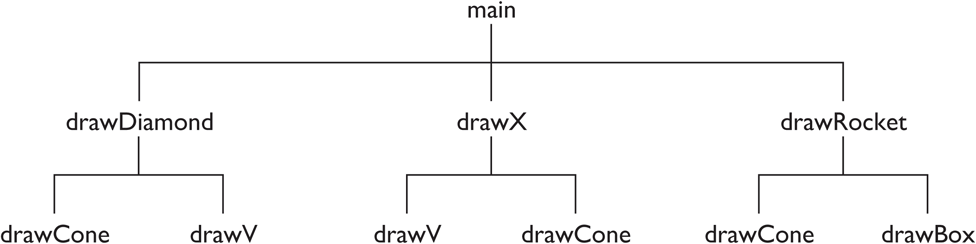
\includegraphics[width=\maxwidth,height=\maxheight,keepaspectratio,alt={Image}]{Figures/img_p95_0.png}}
\end{center}



\begin{verbatim}
 1st  main
 2nd      drawDiamond
 3rd          drawCone
 4th          drawV
 5th      drawX
 6th          drawV
 7th          drawCone
 8th      drawRocket
 9th          drawCone
10th          drawBox
11th          drawBox
12th          drawCone
\end{verbatim}

Hãy nhớ rằng thứ tự mà bạn định nghĩa các phương thức không cần phải
song song với thứ tự chúng được thực thi. Thứ tự thực thi được quyết
định bởi phần thân của phương thức \texttt{main} và bởi các phần thân
của các phương thức được gọi từ \texttt{main}. Một lời khai báo phương
thức tĩnh giống như một mục từ trong từ điển---nó định nghĩa một từ,
nhưng không xác định từ đó sẽ được sử dụng như thế nào. Phần thân của
phương thức \texttt{main} của chương trình này nói rằng hãy thực thi
\texttt{drawDiamond} trước, sau đó \texttt{drawX}, sau đó
\texttt{drawRocket}. Đây là thứ tự thực thi, bất kể thứ tự mà các phương
thức được định nghĩa.

Java cho phép bạn định nghĩa các phương thức theo bất kỳ thứ tự nào bạn
thích. Bắt đầu với \texttt{main} ở trên cùng và đi dần xuống các phương
thức ở cấp độ ngày càng thấp là một cách tiếp cận phổ biến để sử dụng,
nhưng nhiều người thích làm ngược lại, đặt các phương thức cấp thấp ở
đầu và \texttt{main} ở cuối. Java không quan tâm bạn dùng thứ tự nào,
nên bạn có thể tự quyết định và làm điều gì bạn thấy tốt nhất. Dù vậy,
sự nhất quán là quan trọng, để sau này bạn có thể dễ dàng tìm thấy một
phương thức trong một chương trình lớn.

Quan trọng là phải lưu ý rằng các chương trình \texttt{DrawFigures1},
\texttt{DrawFigures2}, và \texttt{DrawFigures3} đều tạo ra kết quả y hệt
nhau ra cửa sổ console. Tuy \texttt{DrawFigures1} có thể là chương trình
dễ đọc nhất đối với người mới bắt đầu, \texttt{DrawFigures2} và đặc biệt
là \texttt{DrawFigures3} có nhiều lợi thế hơn nó. Thứ nhất, một giải
pháp được cấu trúc tốt sẽ dễ hiểu hơn, và bản thân các phương thức trở
thành một phương tiện để giải thích chương trình. Hơn nữa, các chương
trình có các phương thức thì linh hoạt hơn và có thể dễ dàng thích ứng
với các tác vụ tương tự nhưng khác biệt. Bạn có thể lấy bảy phương thức
được định nghĩa trong \texttt{DrawFigures3} và viết một chương trình mới
để tạo ra một đầu ra lớn hơn và phức tạp hơn. Việc xây dựng các phương
thức tĩnh để tạo các lệnh mới làm tăng độ linh hoạt của bạn mà không
thêm vào sự phức tạp không cần thiết. Ví dụ, bạn có thể thay thế phương
thức \texttt{main} bằng một phiên bản gọi các phương thức khác theo thứ
tự mới sau đây. Nó sẽ tạo ra kết quả gì?

\begin{verbatim}
public static void main(String[] args) {
    drawCone();
    drawCone();
    drawRocket();
    drawX();
    drawRocket();
    drawDiamond();
    drawBox();
    drawDiamond();
    drawX();
    drawRocket();
}
\end{verbatim}

\subsection{Tóm tắt Chương (Chapter
Summary)}\label{tuxf3m-tux1eaft-chux1b0ux1a1ng-chapter-summary}

\begin{itemize}
\tightlist
\item
  Máy tính thực thi các tập hợp lệnh được gọi là chương trình
  (programs). Máy tính lưu trữ thông tin nội bộ dưới dạng chuỗi các số 0
  và số 1 (số nhị phân - binary numbers).
\item
  Ngành lập trình và khoa học máy tính xử lý các thuật toán
  (algorithms), đó là các mô tả từng bước để giải quyết vấn đề.
\item
  Java là một ngôn ngữ lập trình hướng đối tượng hiện đại được Sun
  Microsystems phát triển, nay thuộc sở hữu của Tập đoàn Oracle, ngôn
  ngữ này có một tập hợp thư viện lớn mà bạn có thể sử dụng để xây dựng
  các chương trình phức tạp.
\item
  Một chương trình được dịch từ văn bản thành các lệnh máy tính bởi một
  chương trình khác gọi là trình biên dịch (compiler). Trình biên dịch
  của Java chuyển đổi các chương trình Java thành một định dạng đặc biệt
  gọi là mã byte (Java bytecodes), mã này được thực thi bằng một chương
  trình đặc biệt gọi là Môi trường Thực thi Java (Java Runtime
  Environment).
\item
  Các lập trình viên Java thường hoàn thành công việc của mình bằng cách
  sử dụng một chương trình soạn thảo được gọi là Môi trường Phát triển
  Tích hợp (Integrated Development Environment - IDE). Các lệnh có thể
  khác nhau tùy từng môi trường, nhưng một quá trình ba bước tương tự
  luôn luôn được sử dụng:

  \begin{enumerate}
  \def\labelenumi{\arabic{enumi}.}
  \tightlist
  \item
    Nhập một chương trình dưới dạng một lớp Java (Java class).
  \item
    Biên dịch (Compile) file chương trình.
  \item
    Chạy (Run) phiên bản đã biên dịch của chương trình.
  \end{enumerate}
\item
  Java sử dụng một lệnh tên là \texttt{System.out.println} để hiển thị
  văn bản trên màn hình console.
\item
  Từ ngữ viết trong một chương trình có thể mang các ý nghĩa khác nhau.
  Từ khóa (Keywords) là các từ dành riêng đặc biệt, là một phần của ngôn
  ngữ. Định danh (Identifiers) là các từ được lập trình viên định nghĩa
  để đặt tên cho các thực thể trong chương trình. Từ cũng có thể được
  đặt vào chuỗi ký tự (strings), đó là các đoạn văn bản có thể được in
  ra console.
\item
  Các chương trình Java sử dụng khoảng trắng và bố cục hợp lý sẽ dễ đọc
  hơn đối với các lập trình viên. Tính dễ đọc cũng được nâng cao bằng
  cách viết các chú ý gọi là chú thích (comments) vào bên trong chương
  trình.
\item
  Ngôn ngữ Java có một cú pháp (syntax), hay một tập hợp các lệnh hợp lệ
  có thể được sử dụng. Một chương trình Java không tuân theo đúng cú
  pháp sẽ không biên dịch được. Một chương trình biên dịch thành công
  nhưng được viết sai vẫn có thể chứa các lỗi gọi là biệt lệ
  (exceptions) xảy ra khi chương trình chạy. Loại lỗi thứ ba là lỗi
  logic hoặc lỗi ý định (intent error). Loại lỗi này xảy ra khi chương
  trình chạy nhưng không làm được điều mà lập trình viên dự định.
\item
  Lệnh trong chương trình được gọi là các câu lệnh (statements). Một lớp
  có thể nhóm các câu lệnh thành các lệnh lớn hơn gọi là các phương thức
  tĩnh (static methods). Phương thức tĩnh giúp lập trình viên nhóm mã
  vào các phần có thể tái sử dụng. Một phương thức tĩnh quan trọng bắt
  buộc phải có trong mọi chương trình được gọi là \texttt{main}.
\item
  Nâng cấp lặp (Iterative enhancement) là quá trình xây dựng một chương
  trình từng phần một, kiểm thử chương trình ở mỗi bước trước khi tiến
  lên bước tiếp theo.
\item
  Các nhiệm vụ lập trình phức tạp nên được chia nhỏ thành các nhiệm vụ
  chính mà máy tính phải thực hiện. Quá trình này được gọi là phân rã
  thủ tục (procedural decomposition). Sử dụng đúng các phương thức tĩnh
  hỗ trợ việc phân rã thủ tục.
\end{itemize}

\subsection{Bài tập Tự kiểm tra (Self-Check
Problems)}\label{buxe0i-tux1eadp-tux1ef1-kiux1ec3m-tra-self-check-problems}

\subsubsection{Mục 1.1: Các Khái niệm Máy tính Cơ bản (Basic Computing
Concepts)}\label{mux1ee5c-1.1-cuxe1c-khuxe1i-niux1ec7m-muxe1y-tuxednh-cux1a1-bux1ea3n-basic-computing-concepts}

\begin{enumerate}
\def\labelenumi{\arabic{enumi}.}
\tightlist
\item
  Tại sao máy tính lại sử dụng số nhị phân (binary numbers)?
\item
  Chuyển đổi từng số thập phân sau đây thành số nhị phân tương đương của
  nó:

  \begin{enumerate}
  \def\labelenumii{\alph{enumii}.}
  \tightlist
  \item
    6
  \item
    44
  \item
    72
  \item
    131
  \end{enumerate}
\item
  Số thập phân tương đương của từng số nhị phân sau đây là gì?

  \begin{enumerate}
  \def\labelenumii{\alph{enumii}.}
  \tightlist
  \item
    100
  \item
    1011
  \item
    101010
  \item
    1001110
  \end{enumerate}
\item
  Bằng lời của bạn, hãy mô tả một thuật toán (algorithm) để nướng bánh
  quy. Giả sử rằng bạn có một số lượng lớn bạn bè đang đói, vì vậy bạn
  sẽ muốn tạo ra nhiều mẻ bánh quy!
\item
  Sự khác biệt giữa file \texttt{MyProgram.java} và file
  \texttt{MyProgram.class} là gì?
\end{enumerate}

\subsubsection{Mục 1.2: Và Bây giờ---Java (And
Now---Java)}\label{mux1ee5c-1.2-vuxe0-buxe2y-giux1eddjava-and-nowjava}

\begin{enumerate}
\def\labelenumi{\arabic{enumi}.}
\setcounter{enumi}{5}
\item
  Những từ nào sau đây có thể được sử dụng trong một chương trình Java
  như là các định danh (identifiers)?

\begin{verbatim}
println         first-name   AnnualSalary   "hello"   ABC
42isTheAnswer   for          sum_of_data    _average  B4
\end{verbatim}
\item
  Cú pháp nào sau đây là đúng để xuất ra một thông báo?

  \begin{enumerate}
  \def\labelenumii{\alph{enumii}.}
  \tightlist
  \item
    \texttt{System.println(Hello,\ world!);}
  \item
    \texttt{System.println.out(\textquotesingle{}Hello,\ world!\textquotesingle{});}
  \item
    \texttt{System.println("Hello,\ world!");}
  \item
    \texttt{System.out.println("Hello,\ world!");}
  \item
    \texttt{Out.system.println"(Hello,\ world!)";}
  \end{enumerate}
\item
  Đầu ra được tạo ra từ các câu lệnh sau là gì?

\begin{verbatim}
System.out.println("\"Quotes\"");
System.out.println("Slashes \\//");
System.out.println("How '\"confounding' \"\\\" it is!");
\end{verbatim}
\item
  Đầu ra được tạo ra từ các câu lệnh sau là gì?

\begin{verbatim}
System.out.println("name\tage\theight");
System.out.println("Archie\t17\t5'9\"");
System.out.println("Betty\t17\t5'6\"");
System.out.println("Jughead\t16\t6'");
\end{verbatim}
\item
  Đầu ra được tạo ra từ các câu lệnh sau là gì?

\begin{verbatim}
System.out.println("Shaq is 7'1");
System.out.println("The string \"\" is an empty message.");
System.out.println("\\'\"\"");
\end{verbatim}
\item
  Đầu ra được tạo ra từ các câu lệnh sau là gì?

\begin{verbatim}
System.out.println("\ta\tb\tc");
System.out.println("\\\\");
System.out.println("'");
System.out.println("\"\"\"");
System.out.println("C:\nin\the downward spiral");
\end{verbatim}
\item
  Đầu ra được tạo ra từ các câu lệnh sau là gì?

\begin{verbatim}
System.out.println("Dear \"DoubleSlash\" magazine,");
System.out.println();
System.out.println("\tYour publication confuses me. Is it");
System.out.println("a \\\\ slash or a //// slash?");
System.out.println("\nSincerely,");
System.out.println("Susan \"Suzy\" Smith");
\end{verbatim}
\item
  Chuỗi lệnh \texttt{println} nào sẽ tạo ra đầu ra sau đây?

\begin{verbatim}
"Several slashes are sometimes seen,"
said Sally. "I've said so." See?
\ / \\ // \\\ ///
\end{verbatim}
\item
  Chuỗi lệnh \texttt{println} nào sẽ tạo ra đầu ra sau đây?

\begin{verbatim}
This is a test of your
knowledge of "quotes" used
in 'string literals.'
You're bound to "get it right"
if you read the section on
''quotes.''
\end{verbatim}
\item
  Viết một lệnh \texttt{println} tạo ra đầu ra sau:

\begin{verbatim}
/ \ // \\ /// \\\
\end{verbatim}
\item
  Viết lại đoạn mã sau dưới dạng một chuỗi các câu lệnh
  \texttt{System.out.println} tương đương (nghĩa là không có bất kỳ lệnh
  \texttt{System.out.print} nào):

\begin{verbatim}
System.out.print("Twas ");
System.out.print("brillig and the");
System.out.println(" ");
System.out.print(" slithy toves did");
System.out.print(" ");
System.out.println("gyre and");
System.out.println("gimble");
System.out.println();
System.out.println( "in the wabe.");
\end{verbatim}
\item
  Đầu ra của chương trình sau là gì? Lưu ý rằng chương trình có chứa một
  số chú thích (comments).

\begin{verbatim}
 1  public class Commentary {
 2      public static void main(String[] args) {
 3          System.out.println("some lines of code");
 4          System.out.println("have // characters on them");
 5          System.out.println("which means ");  // that they are comments
 6          // System.out.println("written by the programmer.");
 7
 8          System.out.println("lines can also");
 9          System.out.println("have /* and */ characters");
10          /* System.out.println("which represents");
11          System.out.println("a multi-line style");
12          */ System.out.println("of comment.");
13      }
14  }
\end{verbatim}
\end{enumerate}

\subsubsection{Mục 1.3: Lỗi Chương trình (Program
Errors)}\label{mux1ee5c-1.3-lux1ed7i-chux1b0ux1a1ng-truxecnh-program-errors}

\begin{enumerate}
\def\labelenumi{\arabic{enumi}.}
\setcounter{enumi}{17}
\item
  Hãy gọi tên ba lỗi trong chương trình sau:

\begin{verbatim}
1  public MyProgram {
2      public static void main(String[] args) {
3          System.out.println("This is a test of the")
4          System.out.Println("emergency broadcast system.");
5      }
6  }
\end{verbatim}
\item
  Hãy gọi tên bốn lỗi trong chương trình sau:

\begin{verbatim}
1  public class SecretMessage {
2      public static main(string[] args) {
3          System.out.println("Speak friend");
4          System.out.println("and enter);
5
6  }
\end{verbatim}
\item
  Hãy gọi tên bốn lỗi trong chương trình sau:

\begin{verbatim}
 1  public class FamousSpeech
 2      public static void main(String[]) {
 3          System.out.println("Four score and seven years ago,");
 4          System.out.println("our fathers brought forth on");
 5          System.out.println("this continent a new nation");
 6          System.out.println("conceived in liberty,");
 7          System.out.println("and dedicated to the proposition");
 8          System.out.println("that");    /* this part should
 9          System.out.println("all");        really say,
10          System.out.println("men");        "all PEOPLE!" */
11          System.out.println("are";
12          System.out.println("created");
13          System.out.println("equal");
14      }
15  }
\end{verbatim}
\end{enumerate}

\subsection{Bài tập (Exercises)}\label{buxe0i-tux1eadp-exercises}

\begin{enumerate}
\def\labelenumi{\arabic{enumi}.}
\item
  Viết một chương trình Java hoàn chỉnh có tên \texttt{Stewie} để in ra
  kết quả sau:

\begin{verbatim}
//////////////////////
|| Victory is mine! ||
\\\\\\\\\\\\\\\\\\\\\\
\end{verbatim}
\item
  Viết một chương trình Java hoàn chỉnh có tên \texttt{Spikey} để in ra
  kết quả sau:

\begin{verbatim}
  \/
 \\//
\\\///
///\\\
 //\\
  /\
\end{verbatim}
\item
  Viết một chương trình Java hoàn chỉnh có tên \texttt{WellFormed} để in
  ra kết quả sau:

\begin{verbatim}
A well–formed Java program has
a main method with { and }
braces.

A System.out.println statement
has ( and ) and usually a
String that starts and ends
with a " character.
(But we type \" instead!)
\end{verbatim}
\item
  Viết một chương trình Java hoàn chỉnh có tên \texttt{Difference} để in
  ra kết quả sau:

\begin{verbatim}
What is the difference between
a ' and a "? Or between a " and a \"?
One is what we see when we're typing our program.
The other is what appears on the "console."
\end{verbatim}
\item
  Viết một chương trình Java hoàn chỉnh có tên \texttt{MuchBetter} để in
  ra kết quả sau:

\begin{verbatim}
A "quoted" String is
'much' better if you learn
the rules of "escape sequences."
Also, "" represents an empty String.
Don't forget: use \" instead of " !
'' is not the same as "
\end{verbatim}
\item
  Viết một chương trình Java hoàn chỉnh có tên \texttt{Meta} mà đầu ra
  của nó chính là đoạn mã nguồn của một chương trình Java in ra ``Hello,
  world!'' dưới dạng đầu ra.
\item
  Viết một chương trình Java hoàn chỉnh có tên \texttt{Mantra} để in ra
  kết quả sau. Hãy sử dụng ít nhất một phương thức tĩnh ngoài
  \texttt{main}.

\begin{verbatim}
There's one thing every coder must understand:
The System.out.println command.
There's one thing every coder must understand:
The System.out.println command.
\end{verbatim}
\item
  Viết một chương trình Java hoàn chỉnh có tên \texttt{Stewie2} để in ra
  kết quả sau. Hãy sử dụng ít nhất một phương thức tĩnh ngoài
  \texttt{main}.

\begin{verbatim}
//////////////////////
|| Victory is mine! ||
\\\\\\\\\\\\\\\\\\\\\\
|| Victory is mine! ||
\\\\\\\\\\\\\\\\\\\\\\
|| Victory is mine! ||
\\\\\\\\\\\\\\\\\\\\\\
|| Victory is mine! ||
\\\\\\\\\\\\\\\\\\\\\\
|| Victory is mine! ||
\\\\\\\\\\\\\\\\\\\\\\
\end{verbatim}
\item
  Viết một chương trình có tên \texttt{Egg} hiển thị đầu ra như sau:

\begin{verbatim}
   _______ 
  /       \ 
 /         \ 
 -"-'-"-'-"- 
 \         / 
  \_______/
\end{verbatim}
\item
  Sửa đổi chương trình từ bài tập trước để trở thành một chương trình
  mới \texttt{Egg2} hiển thị đầu ra như sau. Sử dụng các phương thức
  tĩnh sao cho phù hợp.

\begin{verbatim}
  _______
 /       \
/         \
\         /
 \_______/
-"-'-"-'-"-
  _______
 /       \
/         \
\         /
 \_______/
-"-'-"-'-"-
\         /
 \_______/
  _______
 /       \
/         \
-"-'-"-'-"-
\         /
 \_______/
\end{verbatim}
\end{enumerate}

\subsubsection{Định danh và Từ khóa (Identifiers and
Keywords)}\label{ux111ux1ecbnh-danh-vuxe0-tux1eeb-khuxf3a-identifiers-and-keywords}

Các từ được sử dụng để đặt tên cho các phần của một chương trình Java
được gọi là \textbf{định danh (identifiers)}.

\begin{quote}
\textbf{Định danh (Identifier)} Một cái tên được đặt cho một thực thể
trong một chương trình, chẳng hạn như một lớp hoặc một phương thức.
\end{quote}

Định danh phải bắt đầu bằng một chữ cái, theo sau có thể là bất kỳ số
lượng chữ cái hoặc chữ số nào. Các ví dụ sau đây đều là các định danh
hợp lệ: \texttt{first}, \texttt{hiThere}, \texttt{numStudents},
\texttt{TwoBy4}

Đặc tả ngôn ngữ Java (Java language specification) định nghĩa tập hợp
các chữ cái bao gồm cả dấu gạch dưới và ký tự đô la (\texttt{\_} và
\texttt{\$}), có nghĩa là các ví dụ sau cũng là các định danh hợp lệ:
\texttt{two\_plus\_two}, \texttt{\_count}, \texttt{\$2donuts},
\texttt{MAX\_COUNT}

Các ví dụ sau đây là các định danh không hợp lệ: \texttt{two+two},
\texttt{hi\ there}, \texttt{hi-There}, \texttt{2by4}

Java có các quy ước về việc viết hoa được các lập trình viên tuân thủ
khá nhất quán. Tất cả các tên lớp nên bắt đầu bằng một chữ cái viết hoa,
như với các lớp \texttt{Hello}, \texttt{Hello2} và \texttt{Hello3} đã
giới thiệu trước đó. Tên của các phương thức nên bắt đầu bằng chữ cái
viết thường, như trong phương thức \texttt{main}. Khi bạn ghép một số từ
lại với nhau để tạo thành một tên lớp hoặc phương thức, hãy viết hoa chữ
cái đầu tiên của mỗi từ sau từ đầu tiên. Trong chương tiếp theo, chúng
ta sẽ thảo luận về các hằng số (constants), có một quy tắc viết hoa
khác, với tất cả các chữ cái đều viết hoa và các từ được phân tách bằng
dấu gạch dưới.

Những quy tắc khác nhau này có vẻ như là những ràng buộc tẻ nhạt, nhưng
việc sử dụng viết hoa nhất quán trong mã của bạn cho phép người đọc
nhanh chóng nhận ra các phần tử mã khác nhau.

Ví dụ, giả sử bạn định ghép các từ ``all my children'' thành một định
danh. Kết quả sẽ là: - \texttt{AllMyChildren} cho một tên lớp (mỗi từ
bắt đầu bằng một chữ in hoa) - \texttt{allMyChildren} cho một tên phương
thức (bắt đầu bằng chữ in thường, các từ tiếp theo viết hoa chữ cái đầu)
- \texttt{ALL\_MY\_CHILDREN} cho tên một hằng số (tất cả viết hoa, các
từ cách nhau bằng dấu gạch dưới; được mô tả trong Chương 2)

Java phân biệt chữ hoa chữ thường (case sensitive), vì vậy các định danh
\texttt{class}, \texttt{Class}, \texttt{CLASS} và \texttt{cLASs} đều
được coi là khác nhau. Hãy ghi nhớ điều này khi bạn đọc\ldots{}

\emph{(Hình ảnh)}

các thông báo lỗi từ trình biên dịch. Con người rất giỏi trong việc hiểu
những gì bạn viết, ngay cả khi bạn viết sai chính tả các từ hoặc mắc
những sai lầm nhỏ như thay đổi chữ hoa chữ thường của một từ. Tuy nhiên,
những sai lầm như thế này khiến trình biên dịch Java trở nên vô cùng bối
rối.

Đừng ngần ngại sử dụng các định danh dài. Tên của bạn càng mang tính mô
tả (descriptive), mọi người (bao gồm cả bạn) sẽ càng dễ đọc chương trình
của bạn hơn. Các định danh có tính mô tả rất đáng để bỏ thời gian gõ. Ví
dụ, lớp \texttt{String} của Java có một phương thức tên là
\texttt{compareToIgnoreCase}.

Tuy nhiên, hãy lưu ý rằng Java có một tập hợp các định danh được xác
định trước gọi là các \textbf{từ khóa (keywords)} được dành riêng cho
các mục đích cụ thể. Trong quá trình đọc cuốn sách này, bạn sẽ học nhiều
từ khóa này và công dụng của chúng. Bạn chỉ có thể sử dụng các từ khóa
cho các mục đích đã định của chúng. Bạn phải cẩn thận tránh sử dụng
những từ này trong tên của các định danh. Ví dụ, nếu bạn đặt tên cho một
phương thức là \texttt{short} hoặc \texttt{try}, điều này sẽ gây ra vấn
đề, vì \texttt{short} và \texttt{try} là các từ khóa dành riêng. Bảng
1.4 hiển thị danh sách đầy đủ các từ khóa dành riêng.

\emph{(Bảng 1.4: Danh sách các từ khóa Java)}

\subsubsection{Một Ví dụ Phức tạp: DrawFigures1 (A Complex
Example)}\label{mux1ed9t-vuxed-dux1ee5-phux1ee9c-tux1ea1p-drawfigures1-a-complex-example}

Lệnh \texttt{println} có thể được sử dụng để vẽ các hình bằng văn bản
dưới dạng đầu ra. Hãy xem xét ví dụ chương trình phức tạp hơn sau đây
(lưu ý rằng nó sử dụng hai lệnh \texttt{println} rỗng để tạo ra các dòng
trống):

\begin{verbatim}
 1  public class DrawFigures1 {
 2      public static void main(String[] args) {
 3          System.out.println("   /\\");
 4          System.out.println("  /  \\");
 5          System.out.println(" /    \\");
 6          System.out.println(" \\    /");
 7          System.out.println("  \\  /");
 8          System.out.println("   \\/");
 9          System.out.println();
10          System.out.println(" \\    /");
11          System.out.println("  \\  /");
12          System.out.println("   \\/");
13          System.out.println("   /\\");
14          System.out.println("  /  \\");
15          System.out.println(" /    \\");
16          System.out.println();
17          System.out.println("   /\\");
18          System.out.println("  /  \\");
19          System.out.println(" /    \\");
20          System.out.println("+------+");
21          System.out.println("|      |");
22          System.out.println("|      |");
23          System.out.println("+------+");
24          System.out.println("|United|");
25          System.out.println("|States|");
26          System.out.println("+------+");
27          System.out.println("|      |");
28          System.out.println("|      |");
29          System.out.println("+------+");
30          System.out.println("   /\\");
31          System.out.println("  /  \\");
32          System.out.println(" /    \\");
33      }
34  }
\end{verbatim}

Sau đây là đầu ra mà chương trình tạo ra. Lưu ý rằng chương trình bao
gồm các ký tự gạch chéo ngược kép
(\texttt{\textbackslash{}\textbackslash{}}), nhưng đầu ra có các ký tự
gạch chéo ngược đơn. Đây là một ví dụ về \textbf{trình tự thoát (escape
sequence)}, như đã được mô tả trước đó.

\begin{verbatim}
   /\ 
  /  \ 
 /    \ 
 \    / 
  \  / 
   \/ 

 \    / 
  \  / 
   \/ 
   /\ 
  /  \ 
 /    \ 

   /\ 
  /  \ 
 /    \ 
+------+ 
|      | 
|      | 
+------+ 
|United| 
|States| 
+------+ 
|      | 
|      | 
+------+ 
   /\ 
  /  \ 
 /    \
\end{verbatim}

\subsubsection{Chú thích và Tính dễ đọc (Comments and
Readability)}\label{chuxfa-thuxedch-vuxe0-tuxednh-dux1ec5-ux111ux1ecdc-comments-and-readability}

Java là một ngôn ngữ có định dạng tự do (free-format language). Điều này
có nghĩa là bạn có thể đưa vào bao nhiêu khoảng trắng và dòng trống tùy
thích, miễn là bạn đặt ít nhất một khoảng trắng hoặc dấu câu khác giữa
các từ. Tuy nhiên, bạn nên nhớ rằng bố cục của một chương trình có thể
nâng cao (hoặc làm giảm đi) tính dễ đọc (readability) của nó. Chương
trình sau đây là hợp lệ nhưng khó đọc:

\begin{verbatim}
1  public class Ugly{public static void main(String[] args)
2  {System.out.println("How short I am!");}}
\end{verbatim}

Dưới đây là một số quy tắc đơn giản nên tuân theo sẽ làm cho chương
trình của bạn dễ đọc hơn: - Đặt các tiêu đề lớp (class headers) và
phương thức (method headers) trên các dòng riêng biệt. - Đặt không quá
một câu lệnh (statement) trên mỗi dòng. - Thụt lề chương trình của bạn
một cách hợp lý. Khi xuất hiện dấu ngoặc nhọn mở, hãy tăng mức thụt lề
của các dòng theo sau nó. Khi xuất hiện dấu ngoặc nhọn đóng, hãy giảm
lùi lề. Thụt lề các câu lệnh bên trong cặp ngoặc nhọn một khoảng trống
nhất quán (một lựa chọn phổ biến là bốn khoảng trắng cho mỗi mức thụt
lề). - Sử dụng các dòng trống để phân tách các phần của chương trình (ví
dụ: các phương thức).

Sử dụng các quy tắc này để viết lại chương trình \texttt{Ugly} mang lại
mã sau:

\begin{verbatim}
1  public class Ugly {
2      public static void main(String[] args) {
3          System.out.println("How short I am!");
4      }
5   }
\end{verbatim}

Các chương trình Java được viết tốt có thể khá dễ đọc, nhưng bạn thường
sẽ muốn đưa vào một số lời giải thích không phải là một phần của bản
thân chương trình. Bạn có thể chú thích (annotate) các chương trình bằng
cách đưa các ghi chú được gọi là \textbf{chú thích (comments)} vào trong
chúng.

\begin{quote}
\textbf{Chú thích (Comment)} Văn bản mà các lập trình viên đưa vào một
chương trình để giải thích mã code của họ. Trình biên dịch (compiler) sẽ
bỏ qua các chú thích.
\end{quote}

Có hai dạng chú thích trong Java. Ở dạng đầu tiên, bạn mở chú thích bằng
dấu gạch chéo theo sau là dấu hoa thị và đóng nó bằng dấu hoa thị theo
sau là dấu gạch chéo:

\begin{verbatim}
/* like this */
\end{verbatim}

Bạn không được đặt khoảng trắng giữa dấu gạch chéo và dấu hoa thị:

\begin{verbatim}
/ * this is bad * /
\end{verbatim}

Bạn có thể đặt hầu như bất kỳ văn bản nào bạn muốn, bao gồm nhiều dòng,
vào trong chú thích:

\begin{verbatim}
/* Thaddeus Martin
   Assignment #1
   Instructor: Professor Walingford
   Grader:     Bianca Montgomery      */
\end{verbatim}

Thứ duy nhất bạn không được phép đặt bên trong một chú thích là các ký
tự kết thúc chú thích. Mã sau đây không hợp lệ:

\begin{verbatim}
/* This comment has an asterisk/slash /*/ in it,
   which prematurely closes the comment. This is bad. */
\end{verbatim}

Java cũng cung cấp một dạng chú thích thứ hai cho các chú thích ngắn
hơn, trên một dòng (single-line comments). Bạn có thể sử dụng hai dấu
gạch chéo liên tiếp để biểu thị rằng phần còn lại của dòng hiện tại (tất
cả mọi thứ bên phải của hai dấu gạch chéo) là một chú thích. Ví dụ, bạn
có thể đặt một chú thích sau một câu lệnh:

\begin{verbatim}
System.out.println("You win!"); // Good job!
\end{verbatim}

Hoặc bạn có thể tạo một chú thích trên một dòng riêng biệt của nó:

\begin{verbatim}
// give an introduction to the user
System.out.println("Welcome to the game of blackjack.");
System.out.println();
System.out.println("Let me explain the rules.");
\end{verbatim}

Bạn thậm chí có thể tạo các khối (blocks) của các chú thích trên một
dòng:

\begin{verbatim}
// Thaddeus Martin
// Assignment #1
// Instructor:  Professor Walingford
// Grader:      Bianca Montgomery
\end{verbatim}

Một số người thích sử dụng dạng chú thích thứ nhất cho các chú thích kéo
dài nhiều dòng nhưng sử dụng dạng thứ hai an toàn hơn vì bạn không phải
nhớ đóng chú thích. Nó cũng làm cho chú thích nổi bật hơn. Đây là một
trường hợp khác mà, nếu giảng viên của bạn không yêu cầu bạn sử dụng một
kiểu chú thích cụ thể, bạn nên tự quyết định kiểu nào bạn thích hơn và
sử dụng nó nhất quán.

Đừng nhầm lẫn giữa chú thích (comments) và văn bản của các lệnh
\texttt{println}. Văn bản trong chú thích của bạn sẽ không được hiển thị
làm đầu ra khi chương trình thực thi. Chú thích chỉ ở đó để giúp người
đọc kiểm tra và hiểu chương trình.

Nên bao gồm các chú thích ở đầu mỗi file class để cho biết class đó thực
hiện chức năng gì. Bạn cũng có thể muốn cung cấp thông tin về việc bạn
là ai, bạn đang học khóa học nào, tên của giáo viên hướng dẫn hoặc người
chấm điểm của bạn, ngày tháng, v.v. Bạn cũng nên chú thích từng phương
thức để giải thích chức năng của nó.

Việc ghi chú thích trở nên hữu ích hơn trong các chương trình lớn hơn và
phức tạp hơn, cũng như trong các chương trình sẽ được xem xét hoặc sửa
đổi bởi nhiều lập trình viên. Những chú thích rõ ràng cực kỳ hữu ích để
giải thích cho người khác, hoặc cho chính bạn vào lúc khác, rằng chương
trình của bạn đang làm gì và tại sao nó làm điều đó.

Bên cạnh hai dạng chú thích đã thảo luận, Java còn hỗ trợ một kiểu chú
thích cụ thể được gọi là chú thích \textbf{Javadoc}. Định dạng của chúng
phức tạp hơn, nhưng chúng có ưu điểm là bạn có thể sử dụng một chương
trình để trích xuất các chú thích để tạo thành các file HTML có thể đọc
được bằng trình duyệt web. Chú thích Javadoc hữu ích trong lập trình
nâng cao hơn và được thảo luận chi tiết hơn trong Phụ lục B.

\emph{(Hình ảnh)}

\subsection{Lỗi chương trình (Program
Errors)}\label{lux1ed7i-chux1b0ux1a1ng-truxecnh-program-errors}

Năm 1949, Maurice Wilkes, một người tiên phong thuở đầu trong ngành máy
tính, đã bày tỏ một quan điểm mà cho đến ngày nay vẫn còn đúng:
\textgreater{} Ngay khi chúng tôi bắt đầu lập trình, chúng tôi đã ngạc
nhiên khi phát hiện ra rằng việc viết cho chương trình chạy đúng không
hề dễ dàng như chúng tôi tưởng. Quá trình gỡ lỗi (debugging) đã phải
được khám phá ra. Tôi có thể nhớ lại khoảnh khắc chính xác khi tôi nhận
ra rằng một phần lớn cuộc đời mình kể từ lúc đó trở đi sẽ là dành để tìm
ra những sai sót trong các chương trình của chính tôi.

Bạn cũng sẽ phải đối mặt với thực tế này khi bạn học lập trình. Bạn sẽ
phạm những sai lầm, giống như bất kỳ lập trình viên nào khác trong lịch
sử, và bạn sẽ cần các chiến lược để loại bỏ những sai lầm đó. Thật may
là, bản thân máy tính có thể giúp bạn làm một số phần việc.

Có ba loại lỗi bạn sẽ gặp khi bạn viết các chương trình: 1. \textbf{Lỗi
cú pháp (Syntax errors)} xảy ra khi bạn sử dụng sai ngôn ngữ Java. Chúng
tương đương với việc dùng sai ngữ pháp và bị trình biên dịch (Java
compiler) bắt lỗi. 2. \textbf{Lỗi logic (Logic errors)} xảy ra khi bạn
viết mã code không thực hiện đúng nhiệm vụ mà nó dự định phải làm. 3.
\textbf{Lỗi thời gian chạy (Runtime errors)} là những lỗi logic nghiêm
trọng đến mức Java ngăn chương trình của bạn tiếp tục thực thi.

\subsubsection{Lỗi Cú pháp (Syntax
Errors)}\label{lux1ed7i-cuxfa-phuxe1p-syntax-errors}

Con người có xu hướng khá bao dung với những sai lầm nhỏ trong lời nói.
Ví dụ, nhân vật Yoda sẽ bị trừ điểm do dùng ngữ pháp khác thường trong
bất kỳ lớp học viết nào, nhưng chúng ta vẫn hiểu ông ấy muốn nói gì.

Trình biên dịch Java sẽ kém bao dung hơn nhiều. Trình biên dịch sẽ báo
cáo các lỗi cú pháp khi nó cố gắng dịch chương trình của bạn từ Java
sang bytecodes nếu chương trình của bạn phá vỡ bất kỳ quy tắc ngữ pháp
nào của Java. Ví dụ, nếu bạn đặt sai vị trí một dấu chấm phẩy trong
chương trình của mình, bạn có thể đẩy trình biên dịch vào sự hỗn loạn
khó gỡ. Trình biên dịch có thể báo cáo một số thông báo lỗi, tùy thuộc
vào việc nó cho rằng có điều gì sai với chương trình của bạn.

Một chương trình sinh ra các lỗi biên dịch (compilation errors) thì
không thể được thực thi. Nếu bạn nộp chương trình của mình cho trình
biên dịch và trình biên dịch báo cáo lỗi, bạn phải sửa chữa lỗi và biên
dịch lại. Bạn sẽ không thể tiến xa hơn cho đến khi chương trình của bạn
không còn lỗi biên dịch.

Một số môi trường phát triển, chẳng hạn như Eclipse, trợ giúp bạn trong
suốt quá trình bằng cách gạch chân các lỗi cú pháp khi bạn viết chương
trình. Điều này giúp bạn dễ dàng phát hiện chính xác vị trí lỗi xảy ra.

Bạn có thể tự đưa ra một lỗi ngay cả trước khi bạn bắt đầu viết chương
trình, nếu bạn chọn sai tên cho file của nó.

\paragraph{LỖI LẬP TRÌNH PHỔ
BIẾN}\label{lux1ed7i-lux1eadp-truxecnh-phux1ed5-biux1ebfn}

\textbf{Tên File Không Khớp Tên Lớp (File Name Does Not Match Class
Name)} Như đã đề cập trước đó, Java yêu cầu tên lớp của một chương trình
và tên file của nó phải khớp với nhau. Ví dụ, một chương trình bắt đầu
với \texttt{public\ class\ Hello} phải được lưu trữ trong một file có
tên \texttt{Hello.java}.

Nếu bạn sử dụng sai tên file (ví dụ, lưu nó dưới tên
\texttt{WrongFileName.java}), bạn sẽ nhận được một thông báo lỗi như thế
này:

\begin{verbatim}
WrongFileName.java:1: error: class Hello is public,
    should be declared in a file named Hello.java
public class Hello {
       ^
1 error
\end{verbatim}

Tên file chỉ là rào cản đầu tiên. Có thể còn có một số lỗi khác xuất
hiện trong chương trình Java của bạn. Một trong những lỗi cú pháp phổ
biến nhất là đánh vần sai một từ (misspell a word). Bạn có thể mắc các
lỗi dấu câu, chẳng hạn như thiếu dấu chấm phẩy. Cũng dễ dàng để quên
toàn bộ một từ, chẳng hạn như một từ khóa (keyword) bắt buộc.

Thông báo lỗi mà trình biên dịch cung cấp có thể hữu ích hoặc không. Nếu
bạn không hiểu nội dung của thông báo lỗi, hãy tìm dấu mũ
(\texttt{\^{}}) bên dưới dòng lệnh, nó chỉ vào vị trí trên dòng nơi mà
trình biên dịch đã gặp rắc rối. Điều này có thể giúp bạn xác định chính
xác vị trí có thể bị thiếu một từ khóa bắt buộc.

\paragraph{LỖI LẬP TRÌNH PHỔ
BIẾN}\label{lux1ed7i-lux1eadp-truxecnh-phux1ed5-biux1ebfn-1}

\textbf{Lỗi Chính tả (Misspelled Words)} Java (cũng như hầu hết các ngôn
ngữ lập trình) rất khắt khe về lỗi chính tả. Bạn cần phải đánh vần từng
từ một cách chính xác, bao gồm cả việc viết hoa thích hợp. Ví dụ, giả sử
rằng bạn sẽ thay thế câu lệnh \texttt{println} trong chương trình
``hello world'' bằng lệnh sau:

\begin{verbatim}
System.out.pruntln("Hello, world!");
\end{verbatim}

Khi bạn thử biên dịch chương trình này, nó sẽ sinh ra một thông báo lỗi
tương tự như sau:

\begin{verbatim}
Hello.java:3: error: cannot find symbol
symbol : method pruntln(java.lang.String)
location: variable out of type PrintStream
        System.out.pruntln("Hello, world!");
                  ^
1 error
\end{verbatim}

Dòng đầu tiên của kết quả này chỉ ra rằng lỗi xảy ra trong file
\texttt{Hello.java} trên dòng số 3 và lỗi đó là trình biên dịch không
thể tìm thấy một biểu tượng (cannot find a symbol). Dòng thứ hai chỉ ra
rằng biểu tượng mà nó không tìm thấy là một phương thức có tên
\texttt{pruntln}. Đó là vì không có phương thức nào như vậy; phương thức
đó được gọi là \texttt{println}. Thông báo lỗi có thể có các dạng hơi
khác nhau tùy thuộc vào những gì bạn đã viết sai chính tả. Ví dụ, bạn có
thể quên không viết hoa từ \texttt{System}:

\begin{verbatim}
system.out.println("Hello, world!");
\end{verbatim}

Bạn sẽ nhận được thông báo lỗi sau:

\begin{verbatim}
Hello.java:3: error: package system does not exist
        system.out.println("Hello, world!");
              ^
1 error
\end{verbatim}

Một lần nữa, dòng đầu tiên cho biết lỗi xảy ra ở dòng 3 của file
\texttt{Hello.java}. Dù vậy, thông báo lỗi ở đây hơi khác, cho biết rằng
nó không thể tìm thấy gói (package) nào có tên là \texttt{system}. Dòng
thứ hai và thứ ba của thông báo lỗi này bao gồm dòng mã gốc với một mũi
tên (dấu mũ) chỉ vào nơi trình biên dịch gặp vấn đề. Lỗi của trình biên
dịch không phải lúc nào cũng rất rõ ràng, nhưng nếu bạn chú ý đến vị trí
mũi tên đang chỉ, bạn sẽ có ý tưởng khá tốt về nơi lỗi xảy ra.

Nếu bạn vẫn không thể tìm ra lỗi, hãy thử xem số dòng của lỗi và so sánh
nội dung của dòng đó với các dòng tương tự trong các chương trình khác.
Bạn cũng có thể nhờ người khác, chẳng hạn như giảng viên hoặc trợ giảng
(lab assistant), kiểm tra giúp chương trình của bạn.

\paragraph{LỖI LẬP TRÌNH PHỔ
BIẾN}\label{lux1ed7i-lux1eadp-truxecnh-phux1ed5-biux1ebfn-2}

\textbf{Quên một Dấu chấm phẩy (Forgetting a Semicolon)} Tất cả các câu
lệnh của Java đều phải kết thúc bằng các dấu chấm phẩy, nhưng bạn rất dễ
quên việc đặt một dấu chấm phẩy ở cuối câu lệnh, như trong chương trình
sau:

\begin{verbatim}
1  public class MissingSemicolon {
2      public static void main(String[] args) {
3           System.out.println("A rose by any other name")
4           System.out.println("would smell as sweet");
5      }
6  }
\end{verbatim}

Trong trường hợp này, trình biên dịch tạo ra đầu ra tương tự như sau:

\begin{verbatim}
MissingSemicolon.java:3: error: ';' expected 
        System.out.println("A rose by any other name") 
                                                     ^ 
1 error
\end{verbatim}

\paragraph{LỖI LẬP TRÌNH PHỔ
BIẾN}\label{lux1ed7i-lux1eadp-truxecnh-phux1ed5-biux1ebfn-3}

\textbf{Quên một Từ khóa Yêu cầu (Forgetting a Required Keyword)} Một
lỗi cú pháp phổ biến khác là quên một từ khóa bắt buộc khi bạn đang gõ
chương trình của mình, chẳng hạn như \texttt{static} hoặc
\texttt{class}. Hãy kiểm tra kỹ chương trình của bạn theo các ví dụ
trong sách giáo khoa để đảm bảo bạn chưa bỏ sót một từ khóa quan trọng
nào. Trình biên dịch sẽ đưa ra các thông báo lỗi khác nhau tùy thuộc vào
việc từ khóa nào bị thiếu, nhưng các thông báo có thể khó hiểu. Ví dụ,
bạn có thể viết một chương trình có tên \texttt{Bug4} và quên từ khóa
\texttt{class} khi viết tiêu đề lớp. Trong trường hợp này, trình biên
dịch sẽ đưa ra thông báo lỗi sau:

\begin{verbatim}
Bug4.java:1: error: class, interface, or enum expected
public Bug4 {
       ^
1 error
\end{verbatim}

Tuy nhiên, nếu bạn quên từ khóa \texttt{void} khi khai báo phương thức
\texttt{main}, trình biên dịch sẽ tạo ra một thông báo lỗi khác:

\begin{verbatim}
Bug5.java:2: error: invalid method declaration; return type required
    public static main(String[] args) {
                  ^
1 error
\end{verbatim}

Một lỗi cú pháp phổ biến khác là quên đóng chuỗi ký tự bằng dấu nháy.
Một nguyên tắc kinh nghiệm hữu ích để làm theo là: lỗi đầu tiên được
trình biên dịch báo cáo là lỗi quan trọng nhất. Các lỗi còn lại có thể
là hậu quả của lỗi đầu tiên đó. Nhiều lập trình viên thậm chí không buồn
quan tâm đến các lỗi phía sau lỗi đầu tiên, bởi vì việc sửa lỗi đầu tiên
và biên dịch lại có thể khiến các lỗi kia biến mất.

\subsubsection{Lỗi logic (Logic Errors hay
Bugs)}\label{lux1ed7i-logic-logic-errors-hay-bugs}

Lỗi logic còn được gọi là rệp (bugs). Các lập trình viên máy tính dùng
các từ như ``đầy rệp'' (bug-ridden) và ``có rệp'' (buggy) để mô tả những
chương trình viết tệ, và quá trình tìm và loại bỏ rệp khỏi các chương
trình được gọi là \textbf{gỡ lỗi (debugging)}.

Từ ``bug'' là một thuật ngữ kỹ thuật cổ xưa có từ trước khi máy tính
xuất hiện; những con ``rệp'' thời kỳ đầu máy tính đôi khi xuất hiện ở cả
phần cứng cũng như phần mềm. Đô đốc Grace Hopper, một người tiên phong
trong ngành máy tính, được coi là người đã phổ biến rộng rãi việc sử
dụng thuật ngữ này trong bối cảnh lập trình máy tính. Bà thường kể lại
một câu chuyện có thật về nhóm các lập trình viên ở trường Đại học
Harvard vào giữa những năm 1940, những người không thể hiểu được chương
trình của mình bị lỗi ở đâu cho tới khi họ mở chiếc máy tính ra và phát
hiện có một con bướm đêm (moth) thật bị mắc kẹt bên trong.

Hình thức của một con bệp có thể đa dạng. Đôi khi, chương trình của bạn
chỉ đơn giản là cư xử không đúng đắn. Ví dụ, nó có thể tạo ra đầu ra
sai. Vào những lúc khác, nó sẽ yêu cầu máy tính thực hiện một nhiệm vụ
rõ ràng là một sự nhầm lẫn, trong trường hợp này, chương trình của bạn
sẽ gặp lỗi thời gian chạy (runtime error) khiến nó phải ngừng thực thi.
Trong chương này, do kiến thức Java của bạn còn hạn chế, nhìn chung loại
lỗi logic duy nhất mà bạn sẽ gặp phải là một sai lầm trong đầu ra của
chương trình do sử dụng câu lệnh \texttt{println} hay lệnh gọi hàm
(method call) không chính xác.

Chúng ta sẽ xem xét một ví dụ về lỗi thời gian chạy ở phần tiếp theo.

\subsection{Phân rã Thủ tục (Procedural
Decomposition)}\label{phuxe2n-ruxe3-thux1ee7-tux1ee5c-procedural-decomposition}

Brian Kernighan, đồng tác giả của cuốn \emph{The C Programming
Language}, đã nói, ``Kiểm soát sự phức tạp là bản chất của lập trình máy
tính.'' Con người chỉ có một khả năng khiêm tốn đối với các chi tiết.
Chúng ta không thể giải quyết những vấn đề phức tạp cùng một lúc. Thay
vào đó, chúng ta cấu trúc việc giải quyết vấn đề của mình bằng cách chia
nhỏ vấn đề thành các phần có thể quản lý được và chinh phục từng phần
một. Chúng ta thường sử dụng thuật ngữ \textbf{phân rã (decomposition)}
để mô tả nguyên tắc này khi áp dụng vào lập trình.

\begin{quote}
\textbf{Phân rã (Decomposition)} Sự chia tách thành các phần có thể nhận
biết được, trong đó mỗi phần đơn giản hơn toàn thể.
\end{quote}

Với các ngôn ngữ lập trình thủ tục (procedural programming languages)
như C, việc phân rã liên quan đến việc chia một nhiệm vụ phức tạp thành
một tập hợp các nhiệm vụ con. Đây là một cách tiếp cận mang định hướng
động từ hoặc hành động rất cao, bao gồm việc chia nhỏ hành động tổng thể
thành một loạt các hành động nhỏ hơn. Kỹ thuật này được gọi là
\textbf{phân rã thủ tục (procedural decomposition)}.

\paragraph{LỖI LẬP TRÌNH PHỔ
BIẾN}\label{lux1ed7i-lux1eadp-truxecnh-phux1ed5-biux1ebfn-4}

\textbf{Không Đóng Chuỗi Ký tự hoặc Chú thích (Not Closing a String
Literal or Comment)} Mỗi chuỗi ký tự phải có một dấu ngoặc kép mở và một
dấu ngoặc kép đóng, nhưng rất dễ quên dấu ngoặc kép đóng. Ví dụ, bạn có
thể viết:

\begin{verbatim}
System.out.println("Hello, world!);
\end{verbatim}

Điều này tạo ra ba thông báo lỗi khác nhau, mặc dù chỉ có một lỗi cú
pháp cơ bản:

\begin{verbatim}
Hello.java:3: error: unclosed string literal
        System.out.println("hello world);
                     ^
Hello.java:3: error: ';' expected
        System.out.println("hello world);
                            ^
Hello.java:5: error: reached end of file while parsing
    }
    ^
3 errors
\end{verbatim}

Trong trường hợp này, thông báo lỗi đầu tiên khá rõ ràng, bao gồm một
mũi tên chỉ vào phần đầu của chuỗi ký tự chưa được đóng. Thông báo lỗi
thứ hai là do nguyên nhân từ lỗi thứ nhất. Vì chuỗi ký tự không được
đóng, trình biên dịch đã không nhận ra dấu ngoặc đơn đóng và dấu chấm
phẩy xuất hiện ở cuối dòng.

Một vấn đề tương tự xảy ra khi bạn quên đóng một chú thích nhiều dòng
bằng cách viết \texttt{*/}, như trong dòng đầu tiên của chương trình
sau:

\begin{verbatim}
/* This is a bad program.
public class Bad {
   public static void main(String[] args){
       System.out.println("Hi there.");
  }
} /* end of program */
\end{verbatim}

File trên không phải là một chương trình; nó là một chú thích dài. Vì
chú thích ở dòng đầu tiên không được đóng, nên toàn bộ chương trình đã
bị nuốt chửng. May mắn thay, nhiều chương trình soạn thảo Java (Java
editor programs) tô màu các phần của một chương trình để giúp bạn nhận
biết chúng bằng mắt thường. Thông thường, nếu bạn quên đóng một chuỗi ký
tự hoặc chú thích, phần còn lại của chương trình của bạn sẽ chuyển sang
màu sai, điều này có thể giúp bạn phát hiện ra lỗi.

Java được thiết kế cho một loại phân rã khác mang định hướng danh từ
hoặc đối tượng (object-oriented) nhiều hơn. Thay vì coi vấn đề như một
loạt các hành động cần thực hiện, chúng ta coi nó như một tập hợp các
đối tượng (objects) phải tương tác với nhau.

Là một nhà khoa học máy tính, bạn nên quen thuộc với cả hai kiểu giải
quyết vấn đề. Cuốn sách này bắt đầu với phân rã thủ tục và dành nhiều
chương để làm chủ các khía cạnh khác nhau của phương pháp tiếp cận thủ
tục. Chỉ sau khi bạn đã thực hành nhuần nhuyễn lập trình thủ tục, chúng
ta mới chuyển sự chú ý trở lại phân rã đối tượng và lập trình hướng đối
tượng.

Như một ví dụ về phân rã thủ tục, hãy xem xét vấn đề nướng một chiếc
bánh (baking a cake). Bạn có thể chia vấn đề này thành các vấn đề con
(subproblems) sau: - Làm bột (Make the batter). - Nướng bánh (Bake the
cake). - Làm kem phủ (Make the frosting). - Phủ kem lên bánh (Frost the
cake).

Mỗi một trong bốn nhiệm vụ này có các chi tiết đi kèm với nó. Ví dụ, để
làm bột, bạn làm theo các bước sau: - Trộn các nguyên liệu khô (Mix the
dry ingredients). - Đánh bông bơ và đường (Cream the butter and sugar).
- Đánh trứng vào (Beat in the eggs). - Khuấy nguyên liệu khô vào (Stir
in the dry ingredients).

Như vậy, bạn chia nhiệm vụ tổng thể thành các nhiệm vụ con, mà bạn lại
tiếp tục chia thành các nhiệm vụ con nhỏ hơn nữa. Cuối cùng, bạn đạt đến
các mô tả đơn giản đến mức không cần giải thích thêm (tức là, các phép
toán nguyên thủy - primitives).

Một sơ đồ một phần của quá trình phân rã này được hiển thị trong Hình
1.2. ``Make cake'' là thao tác ở mức cao nhất. Nó được định nghĩa dựa
trên bốn thao tác ở mức thấp hơn gọi là ``Make batter,'' ``Bake,''
``Make frosting,'' và ``Frost cake.'' Thao tác ``Make batter'' lại được
định nghĩa dựa trên các thao tác ở mức thậm chí thấp hơn nữa, và điều
tương tự có thể được thực hiện cho ba thao tác kia. Sơ đồ này được gọi
là một \textbf{sơ đồ cấu trúc (structure diagram)} và nhằm mục đích chỉ
ra cách một vấn đề được phân tách thành các vấn đề con. Trong sơ đồ này,
bạn cũng có thể biết các thao tác được thực hiện theo thứ tự nào bằng
cách đọc từ trái sang phải. Điều đó không đúng đối với hầu hết các sơ đồ
cấu trúc. Để xác định thứ tự thực tế mà các chương trình con được thực
hiện, bạn thường phải tham chiếu đến bản thân chương trình.

\emph{(Hình 1.2: Phân rã nhiệm vụ ``Make cake'')}

\begin{figure}
\centering


\begin{center}
\pandocbounded{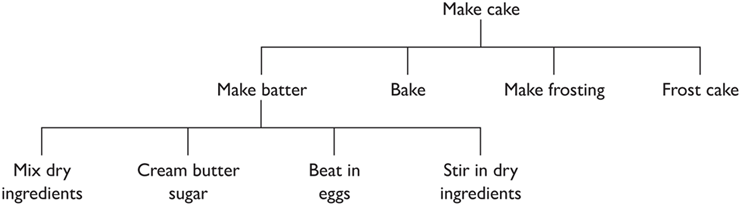
\includegraphics[width=\maxwidth,height=\maxheight,keepaspectratio,alt={Image}]{Figures/img_p65_1.png}}
\end{center}


\caption{Image}
\end{figure}

Một thuật ngữ giải quyết vấn đề cuối cùng liên quan đến quá trình lập
trình. Các lập trình viên chuyên nghiệp phát triển các chương trình theo
từng giai đoạn. Thay vì cố gắng tạo ra một chương trình hoàn chỉnh chạy
được cùng một lúc, họ chọn một phần của vấn đề để cài đặt trước. Sau đó
họ thêm một phần khác, và một phần khác, và một phần khác nữa. Tổng thể
chương trình được xây dựng lên một cách từ từ, từng mảnh một. Quá trình
này được gọi là \textbf{nâng cấp lặp (iterative enhancement)} hoặc
\textbf{tinh chỉnh từng bước (stepwise refinement)}.

\begin{quote}
\textbf{Nâng cấp lặp (Iterative Enhancement)} Quá trình tạo ra một
chương trình theo từng giai đoạn, bổ sung chức năng mới ở mỗi giai đoạn.
Một tính năng quan trọng của mỗi bước lặp là bạn có thể kiểm thử (test)
nó để đảm bảo phần đó hoạt động tốt trước khi chuyển sang bước tiếp
theo.
\end{quote}

Bây giờ, chúng ta hãy xem xét một cấu trúc sẽ cho phép bạn nâng cấp lặp
các chương trình Java của mình để cải thiện cấu trúc của chúng và giảm
bớt sự dư thừa (redundancy): các phương thức tĩnh (static methods).

\subsubsection{Các Phương thức Tĩnh (Static
Methods)}\label{cuxe1c-phux1b0ux1a1ng-thux1ee9c-tux129nh-static-methods}

Java được thiết kế cho các đối tượng (objects), và lập trình trong Java
thường liên quan đến việc phân rã một vấn đề thành các đối tượng khác
nhau, mỗi đối tượng có các phương thức thực hiện những nhiệm vụ cụ thể.
Bạn sẽ thấy cách điều này hoạt động trong các chương sau, nhưng bây giờ,
chúng bản phân rã thủ tục. Chúng ta sẽ hoãn việc xem xét một số chi tiết
của Java lại trong khi chúng ta thảo luận về lập trình nói chung.

Hãy xem xét chương trình sau, vẽ hai hộp văn bản trên cửa sổ console:

\begin{verbatim}
 1  // This program draws two box figures.
 2  public class DrawBoxes {
 3       public static void main(String[] args) {
 4           System.out.println("+------+");
 5           System.out.println("|      |");
 6           System.out.println("|      |");
 7           System.out.println("+------+");
 8           System.out.println();
 9           System.out.println("+------+");
10           System.out.println("|      |");
11           System.out.println("|      |");
12           System.out.println("+------+");
13       }
14   }
\end{verbatim}

\emph{(Hình ảnh minh họa)}

Chương trình hoạt động chính xác, nhưng bốn dòng được dùng để vẽ hộp
xuất hiện hai lần. Sự lặp lại (redundancy) này là không mong muốn vì một
số lý do. Ví dụ, bạn có thể muốn thay đổi hình thức của các hộp, trong
trường hợp đó bạn sẽ phải thực hiện mọi chỉnh sửa hai lần. Ngoài ra, bạn
có thể muốn vẽ thêm các hộp khác, điều này sẽ yêu cầu bạn phải gõ thêm
các bản sao (hoặc copy và paste) các dòng trùng lặp.

Chúng ta có thể cải thiện chương trình bằng cách giới thiệu một lệnh mới
để vẽ cái hộp và sau đó thực thi lệnh đó hai lần. Java không có một lệnh
``vẽ một cái hộp'', nhưng bạn có thể tạo ra một lệnh như vậy. Một lệnh
được đặt tên như vậy được gọi là một \textbf{phương thức tĩnh (static
method)}.

\begin{quote}
\textbf{Phương thức Tĩnh (Static Method)} Một khối (block) các câu lệnh
Java được đặt cho một cái tên.
\end{quote}

Các phương thức tĩnh là các đơn vị của quá trình phân rã thủ tục. Chúng
ta thường chia một lớp (class) thành một vài phương thức tĩnh, mỗi
phương thức giải quyết một phần nào đó của vấn đề tổng thể. Ví dụ, đây
là một phương thức tĩnh để vẽ một cái hộp:

\begin{verbatim}
public static void drawBox() {
    System.out.println("+------+");
    System.out.println("|      |");
    System.out.println("|      |");
    System.out.println("+------+");
}
\end{verbatim}

Bạn đã nhìn thấy một phương thức tĩnh có tên là \texttt{main} trong các
chương trình trước đó. Nhớ lại rằng phương thức \texttt{main} có dạng
sau:

\begin{verbatim}
public static void main(String[] args) {
    <statement>;
    <statement>;
    ...
    <statement>;
}
\end{verbatim}

Các phương thức tĩnh mà bạn sẽ viết có cấu trúc tương tự:

\begin{verbatim}
public static void <name>() {
    <statement>;
    <statement>;
    ...
    <statement>;
}
\end{verbatim}

Dòng đầu tiên được gọi là \textbf{tiêu đề phương thức (method header)}.
Bạn chưa cần phải hiểu đầy đủ ý nghĩa của từng phần trong tiêu đề này
trong Java; hiện tại, chỉ cần nhớ rằng bạn sẽ cần viết
\texttt{public\ static\ void}, theo sau là tên mà bạn muốn đặt cho
phương thức, theo sau là một cặp dấu ngoặc đơn. Nói ngắn gọn, đây là ý
nghĩa của các từ trong tiêu đề: - Từ khóa \texttt{public} cho biết
phương thức này có sẵn để được sử dụng bởi tất cả các phần trong chương
trình của bạn. Mọi phương thức bạn viết sẽ đều là \texttt{public}. - Từ
khóa \texttt{static} cho biết đây là một phương thức tĩnh (theo phong
cách thủ tục, không phải hướng đối tượng). Hiện tại, mọi phương thức bạn
viết sẽ là \texttt{static}, cho đến khi bạn học về định nghĩa đối tượng
trong Chương 8. - Từ khóa \texttt{void} cho biết phương thức này thực
thi các câu lệnh nhưng không tạo ra (trả về) bất kỳ giá trị nào. (Các
phương thức khác mà bạn sẽ thấy sau này tính toán và trả về các giá
trị.) - \texttt{\textless{}name\textgreater{}} (ví dụ: \texttt{drawBox})
là tên của phương thức. - Cặp ngoặc đơn trống xác định một danh sách
(trong trường hợp này, một danh sách trống) các giá trị được gửi tới
phương thức của bạn như là đầu vào; các giá trị như vậy được gọi là
\textbf{tham số (parameters)} và sẽ không được đưa vào các phương thức
của bạn cho đến Chương 3.

Việc bao gồm từ khóa \texttt{static} cho mỗi phương thức bạn định nghĩa
có vẻ cồng kềnh. Các sách giáo khoa Java khác thường không thảo luận về
các phương thức tĩnh sớm như chúng tôi làm ở đây; thay vào đó, họ chỉ ra
các kỹ thuật khác để phân rã vấn đề. Nhưng mặc dù các phương thức tĩnh
cần một chút công sức để tạo ra, chúng là những công cụ mạnh mẽ và hữu
ích để cải thiện các chương trình Java cơ bản.

\emph{(Hình ảnh)}

Sau phần tiêu đề trong phương thức mẫu của chúng ta, một chuỗi các lệnh
\texttt{println} tạo nên \textbf{phần thân (body)} của phương thức tĩnh
này. Giống như trong phương thức \texttt{main}, các câu lệnh của phương
thức này được thực thi theo thứ tự từ đầu đến cuối.

Bằng cách định nghĩa phương thức \texttt{drawBox}, bạn đã gán một cái
tên đơn giản cho chuỗi lệnh \texttt{println} này. Nó giống như việc nói
với trình biên dịch Java, ``Bất cứ khi nào tôi bảo bạn `drawBox', ý tôi
thực sự là bạn nên thực thi các câu lệnh \texttt{println} trong phương
thức \texttt{drawBox}.'' Nhưng lệnh sẽ không thực sự được thực thi trừ
khi phương thức \texttt{main} của chúng ta trình bày rõ ràng
(explicitly) rằng nó muốn làm vậy. Hành động thực thi một phương thức
tĩnh được gọi là \textbf{lời gọi hàm (method call)}.

\begin{quote}
\textbf{Lời gọi Hàm (Method Call)} Một lệnh để thực thi một phương thức
khác, điều này làm cho tất cả các câu lệnh bên trong phương thức đó được
thực thi.
\end{quote}

Để thực thi lệnh \texttt{drawBox}, hãy đưa dòng này vào phương thức
\texttt{main} của chương trình của bạn:

\begin{verbatim}
drawBox();
\end{verbatim}

Do chúng ta muốn thực thi lệnh \texttt{drawBox} hai lần (để vẽ hai hộp),
phương thức \texttt{main} nên chứa hai lời gọi đến phương thức
\texttt{drawBox}. Chương trình sau sử dụng phương thức \texttt{drawBox}
để tạo ra đầu ra giống như chương trình \texttt{DrawBoxes} ban đầu:

\begin{verbatim}
 1  // Draws two box figures using a static method.
 2  public class DrawBoxes2 {
 3      public static void main(String[] args) {
 4          drawBox();
 5          System.out.println();
 6          drawBox();
 7      }
 8
 9      public static void drawBox() {
10          System.out.println("+------+");
11          System.out.println("|      |");
12          System.out.println("|      |");
13          System.out.println("+------+");
14      }
15  }
\end{verbatim}

\subsubsection{Luồng Điều khiển (Flow of
Control)}\label{luux1ed3ng-ux111iux1ec1u-khiux1ec3n-flow-of-control}

Điều khó hiểu nhất về các phương thức tĩnh là các chương trình chứa các
phương thức tĩnh không thực thi tuần tự từ trên xuống dưới. Thay vào đó,
mỗi khi chương trình bắt gặp một lời gọi phương thức tĩnh, việc thực thi
của chương trình ``nhảy'' đến phương thức tĩnh đó, thực thi từng câu
lệnh trong phương thức đó theo thứ tự, và sau đó ``nhảy'' trở lại điểm
bắt đầu của lời gọi và tiếp tục thực thi. Thứ tự mà các câu lệnh của một
chương trình được thực thi được gọi là \textbf{luồng điều khiển (flow of
control)} của chương trình.

\begin{quote}
\textbf{Luồng Điều khiển (Flow of Control)} Thứ tự mà các câu lệnh của
một chương trình Java được thực thi.
\end{quote}

Hãy xem xét luồng điều khiển của chương trình \texttt{DrawBoxes2} hiển
thị trước đó. Nó có hai phương thức. Phương thức đầu tiên là phương thức
quen thuộc \texttt{main}, và phương thức thứ hai là \texttt{drawBox}.
Giống như bất kỳ chương trình Java nào, quá trình thực thi bắt đầu bằng
phương thức \texttt{main}:

\begin{verbatim}
public static void main(String[] args) {
    drawBox();
    System.out.println();
    drawBox();
}
\end{verbatim}

Về một khía cạnh nào đó, quá trình thực thi chương trình này là tuần tự:
Mỗi câu lệnh được liệt kê trong phương thức \texttt{main} được thực thi
lần lượt, từ đầu đến cuối.

Nhưng phương thức \texttt{main} này bao gồm hai lời gọi khác nhau tới
phương thức \texttt{drawBox}. Chương trình này sẽ làm ba việc khác nhau:
thực thi \texttt{drawBox}, thực thi một lệnh \texttt{println}, sau đó
lại thực thi \texttt{drawBox} một lần nữa.

Sơ đồ dưới đây chỉ ra luồng điều khiển do chương trình này sinh ra.

Theo dõi sơ đồ, bạn có thể thấy rằng chín câu lệnh \texttt{println} đã
được thực thi. Đầu tiên bạn chuyển quyền điều khiển cho phương thức
\texttt{drawBox} và thực thi bốn câu lệnh của nó. Sau đó bạn quay trở
lại \texttt{main} và thực thi câu lệnh \texttt{println} của nó. Sau đó
bạn chuyển quyền điều khiển lần thứ hai tới \texttt{drawBox} và một lần
nữa thực thi bốn câu lệnh của nó.

\emph{(Sơ đồ luồng điều khiển)}


\begin{center}
\pandocbounded{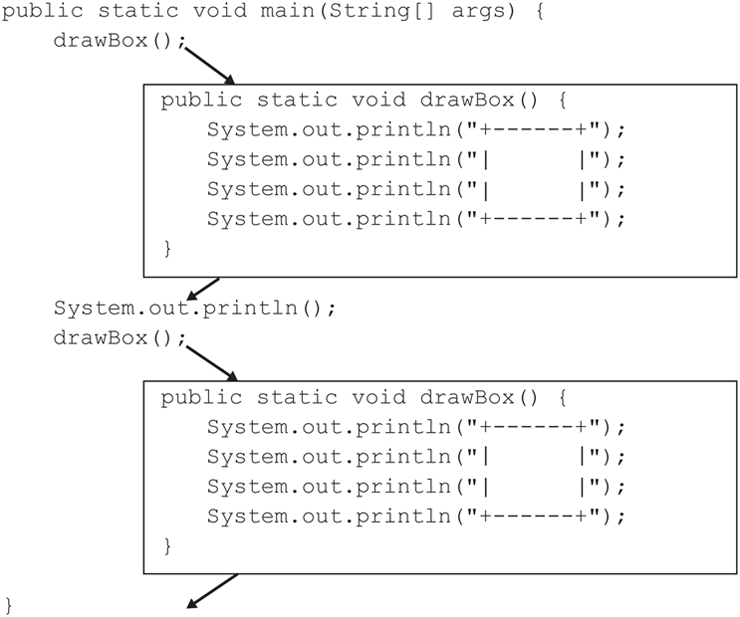
\includegraphics[width=\maxwidth,height=\maxheight,keepaspectratio,alt={Image}]{Figures/img_p75_0.png}}
\end{center}



Việc tạo ra các lời gọi hàm (method calls) này gần giống như sao chép
(copy) và dán (paste) mã của phương thức đó vào trong phương thức
\texttt{main}. Kết quả là, chương trình này có hành vi giống hệt như
phương thức \texttt{main} chín dòng của chương trình \texttt{DrawBoxes}:

\begin{verbatim}
public static void main(String[] args) {
     System.out.println("+------+");
     System.out.println("|      |");
     System.out.println("|      |");
     System.out.println("+------+");
     System.out.println();
     System.out.println("+------+");
     System.out.println("|      |");
     System.out.println("|      |");
     System.out.println("+------+");
}
\end{verbatim}

Phiên bản này đơn giản hơn về mặt luồng điều khiển của nó, nhưng phiên
bản trước tránh được sự lặp lại của việc để cùng một các lệnh
\texttt{println} xuất hiện nhiều lần. Nó cũng mang lại cảm nhận tốt hơn
về cấu trúc của giải pháp. Trong phiên bản gốc, rõ ràng là có một nhiệm
vụ con (subtask) tên là \texttt{drawBox} đang được thực hiện hai lần.
Ngoài ra, mặc dù phiên bản cuối cùng của phương thức \texttt{main} chứa
ít dòng mã hơn chương trình \texttt{DrawBoxes2}, hãy xem xét điều gì sẽ
xảy ra nếu bạn muốn thêm một hộp thứ ba vào đầu ra. Bạn sẽ phải thêm lại
năm lệnh \texttt{println} bắt buộc, trong khi ở các chương trình sử dụng
phương thức \texttt{drawBox}, bạn có thể chỉ cần thêm một lệnh
\texttt{println} nữa và một lời gọi hàm thứ ba.

Java cho phép bạn định nghĩa các phương thức theo bất kỳ thứ tự nào bạn
thích. Có một quy ước phổ biến là đặt phương thức \texttt{main} làm
phương thức đầu tiên hoặc cuối cùng trong lớp (class). Trong cuốn sách
giáo khoa này, chúng tôi thường sẽ đặt \texttt{main} đầu tiên, nhưng các
chương trình sẽ hoạt động tương tự nếu chúng ta đổi chỗ thứ tự. Ví dụ,
chương trình sửa đổi sau đây có hành vi giống hệt như chương trình
\texttt{DrawBoxes2} trước đó:

\begin{verbatim}
 1  // Draws two box figures using a static method.
 2  public class DrawBoxes3 {
 3      public static void drawBox() {
 4          System.out.println("+------+");
 5          System.out.println("|      |");
 6          System.out.println("|      |");
 7          System.out.println("+------+");
 8      }
 9
10      public static void main(String[] args) {
11          drawBox();
12          System.out.println();
13          drawBox();
14      }
15  }
\end{verbatim}

Phương thức \texttt{main} luôn là điểm bắt đầu cho việc thực thi chương
trình, và từ điểm bắt đầu đó, bạn có thể xác định thứ tự mà các phương
thức khác được gọi.

\subsubsection{Các Phương thức Gọi Các Phương thức Khác (Methods That
Call Other
Methods)}\label{cuxe1c-phux1b0ux1a1ng-thux1ee9c-gux1ecdi-cuxe1c-phux1b0ux1a1ng-thux1ee9c-khuxe1c-methods-that-call-other-methods}

Phương thức \texttt{main} không phải là nơi duy nhất bạn có thể gọi một
phương thức khác. Thực tế, bất kỳ phương thức nào cũng có thể gọi bất kỳ
phương thức nào khác. Do đó, luồng điều khiển có thể trở nên khá phức
tạp. Chẳng hạn, hãy xem xét chương trình khá kỳ lạ sau đây. Chúng tôi
chủ đích sử dụng các từ vô nghĩa (``foo,'' ``bar,'' ``baz,'' và
``mumble'') bởi vì chương trình không nhằm mục đích có ý nghĩa.

\begin{verbatim}
 1  public class FooBarBazMumble {
 2      public static void main(String[] args) {
 3          foo();
 4          bar();
 5          System.out.println("mumble");
 6      }
 7
 8      public static void foo() {
 9          System.out.println("foo");
10      }
11
12      public static void bar() {
13          baz();
14          System.out.println("bar");
15      }
16
17      public static void baz() {
18          System.out.println("baz");
19      }
20  }
\end{verbatim}

Bạn khó có thể biết dễ dàng đầu ra mà chương trình này tạo ra, vì vậy
hãy cùng khám phá chi tiết những gì chương trình đang làm. Hãy nhớ rằng
Java luôn bắt đầu với phương thức được gọi là \texttt{main}. Trong
chương trình này, phương thức \texttt{main} gọi phương thức \texttt{foo}
và phương thức \texttt{bar}, sau đó thực thi một lệnh \texttt{println}:

\begin{verbatim}
public static void main(String[] args) {
    foo();
    bar();
    System.out.println("mumble");
}
\end{verbatim}

Mỗi một trong hai lời gọi phương thức này sẽ mở rộng ra thành nhiều câu
lệnh hơn. Hãy xem xét việc mở rộng các lời gọi đến các phương thức
\texttt{foo} và \texttt{bar} trước: Điều này giúp bức tranh về luồng
điều khiển của chúng ta trở nên hoàn chỉnh hơn, nhưng hãy lưu ý rằng
\texttt{bar} lại gọi phương thức \texttt{baz}, vì vậy chúng ta cũng phải
mở rộng phương thức đó nữa.

\emph{(Hình ảnh)}


\begin{center}
\pandocbounded{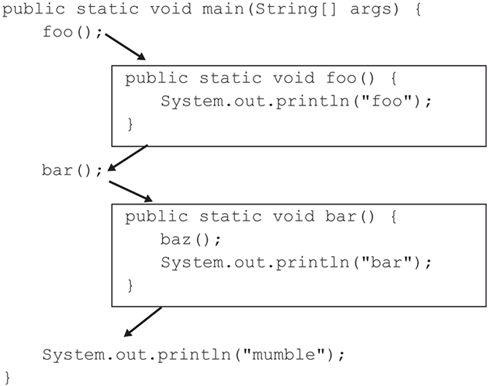
\includegraphics[width=\maxwidth,height=\maxheight,keepaspectratio,alt={Image}]{Figures/img_p80_0.png}}
\end{center}




\providecommand{\pandocbounded}[1]{#1}
\makeatletter
\def\maxwidth{\ifdim\Gin@nat@width>\linewidth\linewidth\else\Gin@nat@width\fi}
\def\maxheight{\ifdim\Gin@nat@height>\textheight\textheight\else\Gin@nat@height\fi}
\makeatother
\providecommand{\tightlist}{\setlength{\itemsep}{0pt}\setlength{\parskip}{0pt}}
\chapter{Dữ liệu nguyên thủy và vòng lặp xác định}
\section{Chương 2: Dữ liệu Nguyên thủy và Vòng lặp Xác định (Primitive
Data and Definite
Loops)}\label{chux1b0ux1a1ng-2-dux1eef-liux1ec7u-nguyuxean-thux1ee7y-vuxe0-vuxf2ng-lux1eb7p-xuxe1c-ux111ux1ecbnh-primitive-data-and-definite-loops}

\subsection{Giới thiệu}\label{giux1edbi-thiux1ec7u}

Bây giờ bạn đã biết đôi chút về cấu trúc cơ bản của một chương trình
Java, bạn đã sẵn sàng để học cách giải quyết các bài toán phức tạp hơn.
Trong thời gian tới, chúng ta sẽ vẫn tập trung vào các chương trình tạo
ra đầu ra (output), nhưng chúng ta sẽ bắt đầu khám phá một số khía cạnh
của lập trình đòi hỏi kỹ năng giải quyết vấn đề.

Nửa đầu của chương này lấp đầy hai mảng quan trọng. Thứ nhất, nó xem xét
các biểu thức (expressions), được sử dụng để thực hiện các tính toán đơn
giản trong Java, đặc biệt là các tính toán liên quan đến dữ liệu số. Thứ
hai, nó thảo luận về các phần tử chương trình được gọi là các biến
(variables) có thể thay đổi giá trị trong khi chương trình thực thi.

Nửa sau của chương giới thiệu cấu trúc điều khiển đầu tiên của bạn: vòng
lặp \texttt{for} (for loop). Bạn sử dụng cấu trúc này để lặp lại các
hành động trong một chương trình. Điều này hữu ích bất cứ khi nào bạn
tìm thấy một khuôn mẫu (pattern) trong một tác vụ, chẳng hạn như việc
tạo ra một hình phức tạp, bởi vì bạn có thể sử dụng một vòng lặp
\texttt{for} để lặp lại hành động nhằm tạo ra khuôn mẫu cụ thể đó. Thử
thách là tìm ra mỗi khuôn mẫu và chỉ ra những hành động lặp lại nào sẽ
tái tạo lại nó.

Vòng lặp \texttt{for} là một cấu trúc điều khiển linh hoạt có thể được
sử dụng cho nhiều tác vụ. Trong chương này, chúng ta sử dụng nó cho các
vòng lặp xác định (definite loops), nơi bạn biết chính xác bạn muốn thực
hiện một tác vụ cụ thể bao nhiêu lần. Trong Chương 5, chúng ta sẽ thảo
luận về cách viết các vòng lặp không xác định (indefinite loops), nơi
bạn không biết trước mình sẽ thực hiện một tác vụ bao nhiêu lần.

\begin{center}\rule{0.5\linewidth}{0.5pt}\end{center}

\subsection{Các khái niệm Dữ liệu Cơ bản (Basic Data
Concepts)}\label{cuxe1c-khuxe1i-niux1ec7m-dux1eef-liux1ec7u-cux1a1-bux1ea3n-basic-data-concepts}

Các chương trình thao tác với thông tin, và thông tin có nhiều dạng.
Java là một ngôn ngữ an toàn kiểu (type-safe language), có nghĩa là nó
yêu cầu bạn phải nêu rõ loại thông tin nào bạn dự định thao tác và nó
đảm bảo rằng bạn thao tác dữ liệu một cách hợp lý. Mọi thứ bạn thao tác
trong một chương trình Java sẽ thuộc một kiểu nhất định và bạn sẽ liên
tục phải báo cho Java biết những kiểu dữ liệu nào bạn dự định sử dụng.

\begin{quote}
\textbf{Kiểu dữ liệu (Data Type)} Tên gọi cho một danh mục các giá trị
dữ liệu có liên quan với nhau, chẳng hạn như kiểu \texttt{int} trong
Java, được sử dụng để biểu diễn các giá trị số nguyên.
\end{quote}

Một quyết định đã được đưa ra ngay từ đầu trong thiết kế của Java là hỗ
trợ hai loại dữ liệu khác nhau: dữ liệu nguyên thủy (primitive data) và
đối tượng (objects). Các nhà thiết kế đã đưa ra quyết định này hoàn toàn
vì lý do hiệu năng, để làm cho các chương trình Java chạy nhanh hơn.
Thật không may, điều đó có nghĩa là bạn phải học hai bộ quy tắc về cách
dữ liệu hoạt động, nhưng đây là một trong những lúc bạn đơn giản là phải
trả giá nếu muốn sử dụng một ngôn ngữ lập trình ở đẳng cấp công nghiệp.
Để làm cho mọi thứ dễ dàng hơn một chút, chúng ta sẽ nghiên cứu các kiểu
dữ liệu nguyên thủy trước tiên, trong chương này; ở chương tiếp theo,
chúng ta sẽ chuyển hướng chú ý sang các đối tượng.

\subsubsection{Các Kiểu Nguyên thủy (Primitive
Types)}\label{cuxe1c-kiux1ec3u-nguyuxean-thux1ee7y-primitive-types}

Có tám kiểu dữ liệu nguyên thủy trong Java: \texttt{boolean},
\texttt{byte}, \texttt{char}, \texttt{double}, \texttt{float},
\texttt{int}, \texttt{long}, và \texttt{short}. Bốn trong số này được
coi là cơ bản: \texttt{boolean}, \texttt{char}, \texttt{double}, và
\texttt{int}. Bốn kiểu còn lại là các biến thể tồn tại cho các chương
trình có yêu cầu đặc biệt.

Bốn kiểu cơ bản mà chúng ta sẽ khám phá được liệt kê trong Bảng 2.1.

\textbf{Bảng 2.1 Các kiểu nguyên thủy thường dùng trong Java} \textbar{}
Kiểu (Type) \textbar{} Mô tả \textbar{} Ví dụ \textbar{}
\textbar---\textbar---\textbar---\textbar{} \textbar{} \texttt{int}
\textbar{} Số nguyên (integer) \textbar{} 42, -3, 0 \textbar{}
\textbar{} \texttt{double} \textbar{} Số thực (real number) \textbar{}
3.14, -0.5 \textbar{} \textbar{} \texttt{char} \textbar{} Ký tự
(character) \textbar{} `a', `X', `!' \textbar{} \textbar{}
\texttt{boolean} \textbar{} Giá trị logic (boolean) \textbar{} true,
false \textbar{}

Các tên kiểu (\texttt{int}, \texttt{double}, \texttt{char}, và
\texttt{boolean}) là các từ khóa (keywords) của Java mà bạn sẽ sử dụng
trong chương trình của mình để cho Trình biên dịch (Compiler) biết rằng
bạn có ý định sử dụng kiểu dữ liệu đó.

Có vẻ kỳ quặc khi sử dụng một kiểu cho số nguyên và một kiểu khác cho số
thực. Chẳng phải mọi số nguyên đều là số thực sao? Câu trả lời là có,
nhưng đây là các loại số hoàn toàn khác nhau. Sự khác biệt lớn đến mức
chúng ta thực hiện sự phân biệt này ngay cả trong tiếng Anh (và tiếng
Việt).

Trong lập trình, sự phân biệt này còn quan trọng hơn, bởi vì số nguyên
và số thực được biểu diễn theo những cách khác nhau trong bộ nhớ của máy
tính: Số nguyên được lưu trữ chính xác (exactly), trong khi số thực được
lưu trữ dưới dạng các giá trị xấp xỉ (approximations) với một số lượng
chữ số có nghĩa giới hạn. Bạn sẽ thấy rằng việc lưu trữ giá trị dưới
dạng xấp xỉ có thể dẫn đến các sai số làm tròn (round-off errors) khi
bạn sử dụng giá trị thực.

\subsection{Biến (Variables)}\label{biux1ebfn-variables}

Dữ liệu nguyên thủy có thể được lưu trữ trong bộ nhớ của máy tính dưới
dạng một biến (variable).

\begin{quote}
\textbf{Biến (Variable)} Một vị trí bộ nhớ có tên và kiểu dùng để lưu
trữ một giá trị.
\end{quote}

Hãy hình dung bộ nhớ của máy tính giống như một bảng tính khổng lồ
(spreadsheet) có nhiều ô nơi dữ liệu có thể được lưu trữ. Khi bạn tạo
một biến trong Java, bạn đang yêu cầu nó dành riêng một trong những ô đó
cho biến mới này. Ban đầu ô sẽ trống, nhưng bạn sẽ có tùy chọn lưu trữ
một giá trị vào ô đó. Và giống như với một bảng tính, bạn sẽ có tùy chọn
thay đổi giá trị trong ô đó sau này.

Tuy nhiên, Java kén chọn hơn một chút so với một bảng tính, ở chỗ nó yêu
cầu bạn phải cho nó biết chính xác loại dữ liệu nào bạn sẽ lưu trữ trong
ô. Ví dụ, nếu bạn muốn lưu trữ một số nguyên, bạn cần cho Java biết rằng
bạn dự định sử dụng kiểu \texttt{int}. Nếu bạn muốn lưu trữ một số thực,
bạn cần cho Java biết rằng bạn dự định sử dụng \texttt{double}. Bạn cũng
phải quyết định một cái tên để sử dụng khi bạn muốn tham chiếu đến vị
trí bộ nhớ này. Các quy tắc thông thường của định danh (identifiers)
trong Java được áp dụng (tên phải bắt đầu bằng một chữ cái, có thể được
theo sau bởi bất kỳ kết hợp nào của chữ cái và chữ số). Quy ước tiêu
chuẩn trong Java là bắt đầu tên biến bằng một chữ cái viết thường, chẳng
hạn như \texttt{number} hoặc \texttt{digits}, và viết hoa bất kỳ từ nào
theo sau, chẳng hạn như \texttt{numberOfDigits}.

Để khám phá việc sử dụng cơ bản của các biến, hãy xem xét một chương
trình tính toán chỉ số khối cơ thể (BMI - body mass index) của một cá
nhân. Các chuyên gia y tế sử dụng con số này để khuyên mọi người về việc
họ có bị thừa cân hay không. Cho trước chiều cao và cân nặng của một cá
nhân, chúngua có thể tính toán BMI của người đó. Khi đó, một chương
trình BMI đơn giản, một cách tự nhiên sẽ có ba biến cho ba mảnh thông
tin này.

Có một vài chi tiết mà chúng ta cần thảo luận về các biến, nhưng việc
nhìn vào một chương trình hoàn chỉnh trước để thấy bức tranh tổng thể có
thể sẽ hữu ích. Chương trình sau tính toán và in ra BMI cho một cá nhân
cao 5 feet 10 inches và nặng 195 pounds:

\begin{verbatim}
 1  // Computes Body Mass Index (BMI) for a specific person.
 2  public class BMICalculator {
 3      public static void main(String[] args) {
 4          // declare variables
 5          double height;
 6          double weight;
 7          double bmi;
 8
 9          // compute BMI
10          height = 70;
11          weight = 195;
12          bmi = weight / (height * height) * 703;
13
14          // print results
15          System.out.println("Current BMI:");
16          System.out.println(bmi);
17      }
18  }
\end{verbatim}

Lưu ý rằng chương trình bao gồm các dòng trống để tách biệt các phần và
các chú thích (comments) để chỉ ra các phần khác nhau của chương trình
làm gì. Nó tạo ra đầu ra (output) như sau:

\begin{verbatim}
Current BMI: 
27.976530612244897
\end{verbatim}

Bây giờ hãy kiểm tra các chi tiết của chương trình này để hiểu cách các
biến hoạt động. Trước khi các biến có thể được sử dụng trong một chương
trình Java, chúng phải được khai báo (declared). Dòng mã khai báo biến
được gọi là khai báo biến (variable declaration).

\begin{quote}
\textbf{Khai báo (Declaration)} Một yêu cầu dành riêng một biến mới với
một tên và một kiểu cho trước.
\end{quote}

Mỗi biến chỉ được khai báo một lần duy nhất. Nếu bạn khai báo một biến
nhiều hơn một lần, bạn sẽ nhận được một thông báo lỗi từ trình biên dịch
Java. Khai báo biến đơn giản có dạng:

\begin{verbatim}
<type> <name>;
\end{verbatim}

chẳng hạn như ba khai báo ở đầu chương trình mẫu của chúng ta:

\begin{verbatim}
double height;
double weight;
double bmi;
\end{verbatim}

Lưu ý rằng một khai báo biến, giống như một câu lệnh (statement), kết
thúc bằng một dấu chấm phẩy (;). Các khai báo này có thể xuất hiện ở bất
cứ nơi nào một câu lệnh có thể xảy ra. Khai báo chỉ định kiểu và tên của
biến. Hãy nhớ rằng tên của mỗi kiểu nguyên thủy là một từ khóa (keyword)
trong Java (\texttt{int}, \texttt{double}, \texttt{char},
\texttt{boolean}). Chúng ta đã sử dụng từ khóa \texttt{double} để định
nghĩa kiểu của ba biến này.

Một khi biến được khai báo, Java dành ra một vị trí bộ nhớ để lưu trữ
giá trị của nó. Tuy nhiên, với dạng khai báo biến đơn giản được sử dụng
trong chương trình của chúng ta, Java không lưu trữ các giá trị ban đầu
vào các vị trí bộ nhớ này. Chúng ta gọi chúng là các biến chưa được khởi
tạo (uninitialized variables), và chúng tương tự như các ô trống trong
một bảng tính:

Vậy làm thế nào để chúng ta đưa các giá trị vào các ô đó? Cách dễ nhất
để làm như vậy là sử dụng một câu lệnh gán (assignment statement). Cú
pháp chung của câu lệnh gán là:

\begin{verbatim}
<variable> = <expression>;
\end{verbatim}

chẳng hạn như:

\begin{verbatim}
height = 70;
\end{verbatim}

Câu lệnh này lưu trữ giá trị \texttt{70} vào vị trí bộ nhớ của biến
\texttt{height}, chỉ ra rằng người này cao 70 inch (5 feet 10 inches).
Chúng ta thường sử dụng cụm từ ``nhận'' (gets) hoặc ``được gán'' (is
assigned) khi đọc một câu lệnh như thế này, chẳng hạn như
``\texttt{height} nhận 70'' hoặc ``\texttt{height} được gán 70''.

Khi câu lệnh thực thi, máy tính trước tiên sẽ đánh giá biểu thức ở phía
bên phải; sau đó, nó lưu trữ kết quả vào vị trí bộ nhớ cho biến đã cho.
Trong trường hợp này, biểu thức chỉ là một giá trị hằng (literal value)
đơn giản, vì vậy sau khi máy tính thực thi câu lệnh này, bộ nhớ trông
như sau:

Lưu ý rằng giá trị được lưu trữ là \texttt{70.0} bởi vì biến này thuộc
kiểu \texttt{double}. Biến \texttt{height} hiện đã được khởi tạo
(initialized), nhưng các biến \texttt{weight} và \texttt{bmi} vẫn chưa
được khởi tạo. Câu lệnh gán thứ hai cung cấp một giá trị cho
\texttt{weight}:

\begin{verbatim}
weight = 195;
\end{verbatim}

Sau khi thực thi câu lệnh này, bộ nhớ trông như sau:

Câu lệnh gán thứ ba bao gồm một công thức (một biểu thức để được đánh
giá):

\begin{verbatim}
bmi = weight / (height * height) * 703;
\end{verbatim}

Để tính giá trị của biểu thức này, máy tính chia cân nặng cho bình
phương của chiều cao và sau đó nhân kết quả của thao tác đó với giá trị
hằng \texttt{703}. Kết quả được lưu vào biến \texttt{bmi}. Do đó, sau
khi máy tính đã thực thi câu lệnh gán thứ ba, bộ nhớ trông như sau:

Hai dòng cuối của chương trình báo cáo kết quả BMI bằng cách sử dụng các
câu lệnh \texttt{println}:

\begin{verbatim}
System.out.println("Current BMI:");
System.out.println(bmi);
\end{verbatim}

Lưu ý rằng chúng ta có thể đưa một biến vào trong một câu lệnh
\texttt{println} giống như cách chúng ta đưa các giá trị hằng và các
biểu thức khác để được in ra.

Như tên gọi của nó, một biến có thể nhận các giá trị khác nhau tại các
thời điểm khác nhau. Ví dụ, hãy xem xét biến thể sau của chương trình
BMI, chương trình này tính toán một BMI mới giả định người đó đã giảm 15
pounds (từ 195 pounds xuống 180 pounds).

\begin{verbatim}
 1   // Computes Body Mass Index (BMI) for two specific people.
 2   public class BMICalculator2 {
 3       public static void main(String[] args) {
 4           // declare variables
 5           double height;
 6           double weight;
 7           double bmi;
 8
 9           // compute BMI
10           height = 70;
11           weight = 195;
12           bmi = weight / (height * height) * 703;
13
14           // print results
15           System.out.println("Previous BMI:");
16           System.out.println(bmi);
17
18           // recompute BMI
19           weight = 180;
20           bmi = weight / (height * height) * 703;
21
22           // report new results
23           System.out.println("Current BMI:");
24           System.out.println(bmi);
25          }
26     }
\end{verbatim}

Chương trình bắt đầu theo cùng một cách, gán cho ba biến các giá trị sau
và báo cáo giá trị ban đầu này của BMI:

Nhưng chương trình mới sau đó bao gồm câu lệnh gán sau:

\begin{verbatim}
weight = 180;
\end{verbatim}

Điều này làm thay đổi giá trị của biến \texttt{weight}:

Bạn có thể nghĩ rằng điều này cũng sẽ thay đổi giá trị của biến
\texttt{bmi}. Rốt cuộc, trước đó trong chương trình chúng ta đã nói rằng
điều sau phải luôn đúng:

\begin{verbatim}
bmi = weight / (height * height) * 703;
\end{verbatim}

Đây là điểm mà sự so sánh với bảng tính (spreadsheet) không còn chính
xác. Một bảng tính có thể lưu trữ các công thức trong các ô của nó và
khi bạn cập nhật một ô, nó có thể làm cho các giá trị trong các ô khác
được cập nhật. Điều này không đúng trong Java.

Bạn cũng có thể bị nhầm lẫn do việc sử dụng dấu bằng cho phép gán. Đừng
nhầm lẫn câu lệnh này với một câu lệnh về sự bằng nhau. Câu lệnh gán
không đại diện cho một mối quan hệ đại số. Trong đại số, bạn có thể nói
\[ x = y + 2 \] Trong toán học, bạn tuyên bố dứt khoát rằng \(x\) bằng
\(y\) cộng hai, một sự thật đúng ở hiện tại và mãi mãi. Nếu \(y\) thay
đổi, \(x\) sẽ thay đổi theo, và ngược lại. Câu lệnh gán của Java rất
khác biệt.

Câu lệnh gán là một lệnh (command) để thực hiện một hành động tại một
thời điểm cụ thể. Nó không đại diện cho một mối quan hệ bền vững giữa
các biến. Đó là lý do tại sao chúng ta thường nói ``nhận'' (gets) hoặc
``được gán'' (is assigned) hơn là nói ``bằng'' (equals) khi chúng ta đọc
các câu lệnh gán.

Trở lại với chương trình, việc đặt lại biến được gọi là \texttt{weight}
không làm đặt lại biến được gọi là \texttt{bmi}. Để tính toán lại
\texttt{bmi} dựa trên giá trị mới cho \texttt{weight}, chúng ta phải bao
gồm câu lệnh gán thứ hai:

\begin{verbatim}
weight = 180;
bmi = weight / (height * height) * 703;
\end{verbatim}

Nếu không, biến \texttt{bmi} sẽ lưu trữ cùng một giá trị như trước. Đó
sẽ là một kết quả khá đáng thất vọng để báo cáo cho một người vừa giảm
15 pounds. Bằng cách bao gồm cả hai câu lệnh này, chúng ta đặt lại cả
biến \texttt{weight} và \texttt{bmi} để bộ nhớ trông như sau:

Đầu ra của phiên bản mới của chương trình là:

\begin{verbatim}
Previous BMI: 
27.976530612244897 
Current BMI: 
25.82448979591837
\end{verbatim}

Một câu lệnh gán rất phổ biến chỉ ra sự khác biệt giữa các mối quan hệ
đại số và các câu lệnh chương trình là:

\begin{verbatim}
x = x + 1;
\end{verbatim}

Hãy nhớ đừng hiểu điều này là ``\(x\) bằng \(x\) cộng 1''. Không có con
số nào thỏa mãn phương trình đó cả. Chúng ta sử dụng một từ như ``nhận''
(gets) để đọc lệnh này là ``\(x\) nhận giá trị của \(x\) cộng thêm 1''.
Điều này có vẻ là một câu lệnh khá kỳ lạ, nhưng bạn có thể giải mã nó
dựa trên các quy tắc đã được vạch ra trước đó. Giả sử giá trị hiện tại
của \texttt{x} là \texttt{19}. Để thực thi câu lệnh, trước tiên bạn đánh
giá biểu thức để thu được kết quả \texttt{20}. Máy tính lưu trữ giá trị
này vào biến có tên ở bên trái, \texttt{x}. Do đó, câu lệnh này cộng
thêm một vào giá trị của biến. Chúng ta gọi đây là phép tăng
(incrementing) giá trị của \texttt{x}. Đây là một thao tác lập trình cơ
bản vì nó tương đương với việc đếm (1, 2, 3, 4, v.v.). Câu lệnh sau đây
là một biến thể đếm ngược, mà chúng ta gọi là phép giảm (decrementing)
một biến:

\begin{verbatim}
x = x - 1;
\end{verbatim}

Chúng ta sẽ thảo luận chi tiết hơn về phép tăng và phép giảm ở phần sau
của chương này.

\subsubsection{Các Biến thể Khai báo/Gán (Assignment/Declaration
Variations)}\label{cuxe1c-biux1ebfn-thux1ec3-khai-buxe1oguxe1n-assignmentdeclaration-variations}

Java là một ngôn ngữ phức tạp cung cấp rất nhiều sự linh hoạt cho các
lập trình viên. Ở phần trước, chúng ta đã thấy dạng đơn giản nhất của
việc khai báo và gán biến, nhưng có nhiều biến thể khác xoay quanh chủ
đề này. Sẽ không phải là một ý tưởng tồi nếu bạn bám vào dạng đơn giản
nhất trong khi bạn đang học, nhưng bạn sẽ bắt gặp các dạng khác khi bạn
đọc các chương trình của người khác, do đó bạn sẽ muốn hiểu chúng có
nghĩa là gì.

Biến thể đầu tiên là Java cho phép bạn cung cấp một giá trị ban đầu cho
một biến tại thời điểm bạn khai báo nó. Cú pháp như sau:

\begin{verbatim}
<type> <name> = <expression>;
\end{verbatim}

chẳng hạn như

\begin{verbatim}
double height = 70;
double weight = 195;
double bmi = weight / (height * height) * 703;
\end{verbatim}

Biến thể này kết hợp khai báo và gán trong một dòng mã. Hai phép gán đầu
tiên có các con số đơn giản sau dấu bằng, nhưng phép gán thứ ba có một
biểu thức phức tạp sau dấu bằng. Ba phép gán này có cùng tác dụng như
việc cung cấp ba khai báo theo sau bởi ba câu lệnh gán:

\begin{verbatim}
double height;
double weight;
double bmi;
height = 70;
weight = 195;
bmi = weight / (height * height) * 703;
\end{verbatim}

Một biến thể khác là khai báo một vài biến có cùng kiểu trong một câu
lệnh duy nhất. Cú pháp là:

\begin{verbatim}
<type> <name>, <name>, <name>, ..., <name>;
\end{verbatim}

chẳng hạn như:

\begin{verbatim}
double height, weight;
\end{verbatim}

Ví dụ này khai báo hai biến khác nhau, cả hai đều thuộc kiểu
\texttt{double}. Lưu ý rằng kiểu chỉ xuất hiện một lần duy nhất, ở phần
đầu của khai báo.

Biến thể cuối cùng là sự pha trộn của hai dạng trước. Bạn có thể khai
báo nhiều biến cùng kiểu, và bạn có thể khởi tạo chúng cùng một lúc. Ví
dụ, bạn có thể viết:

\begin{verbatim}
double height = 70, weight = 195;
\end{verbatim}

Câu lệnh này khai báo hai biến \texttt{double} là \texttt{height} và
\texttt{weight} và cung cấp cho chúng các giá trị ban đầu (tương ứng là
\texttt{70} và \texttt{195}). Java thậm chí còn cho phép bạn kết hợp
việc có khởi tạo và không khởi tạo, chẳng hạn như:

\begin{verbatim}
double height = 70, weight = 195, bmi;
\end{verbatim}

Câu lệnh này khai báo ba biến \texttt{double} được gọi là
\texttt{height}, \texttt{weight}, và \texttt{bmi} và cung cấp các giá
trị ban đầu cho hai trong số chúng (\texttt{height} và \texttt{weight}).
Biến \texttt{bmi} chưa được khởi tạo.

Kể từ Java 10, bạn có thể khai báo kiểu của một biến là \texttt{var} và
trình biên dịch Java sẽ tự động suy luận ra kiểu thích hợp. Ví dụ, các
khai báo:

\begin{verbatim}
var age = 42;
var height = 70.5;
\end{verbatim}

tương đương với:

\begin{verbatim}
int age = 42;
double height = 70.5;
\end{verbatim}

Các tác giả thích phong cách tiêu chuẩn với các kiểu biến được chỉ định
rõ ràng, do đó chúng tôi sẽ không sử dụng \texttt{var} trong các ví dụ
của chúng tôi trong tài liệu này.

\begin{quote}
{[}!WARNING{]} \textbf{LỖI LẬP TRÌNH THƯỜNG GẶP: Khai báo Cùng một Biến
Hai Lần} Một trong những điều cần ghi nhớ khi bạn học là bạn chỉ có thể
khai báo bất kỳ biến nào cho trước đúng một lần duy nhất. Bạn có thể gán
cho nó bao nhiêu lần tùy thích một khi bạn đã khai báo nó, nhưng khai
báo chỉ nên xuất hiện một lần duy nhất. Hãy hình dung việc khai báo biến
giống như việc nhận phòng khách sạn và việc gán giống như việc ra vào
phòng của bạn. Bạn phải nhận phòng trước để lấy chìa khóa phòng, nhưng
sau đó bạn có thể đến và đi thường xuyên như bạn muốn. Nếu bạn cố gắng
nhận phòng lần thứ hai, khách sạn có khả năng sẽ hỏi bạn xem bạn có thực
sự muốn trả tiền cho phòng thứ hai hay không.

Nếu bạn khai báo một biến nhiều hơn một lần, Java sẽ tạo ra một lỗi
trình biên dịch. Ví dụ, giả sử chương trình của bạn chứa các dòng sau:

\begin{verbatim}
int x = 13;
System.out.println(x);
int x = 2;         // this line does not compile
System.out.println(x);
\end{verbatim}

Dòng đầu tiên là ổn. Nó khai báo một biến số nguyên có tên là \texttt{x}
và khởi tạo nó thành \texttt{13}. Dòng thứ hai cũng ổn, bởi vì nó đơn
giản in ra giá trị của \texttt{x}. Nhưng dòng thứ ba sẽ tạo ra một thông
báo lỗi chỉ ra rằng ``\texttt{x} is already defined'' (\texttt{x} đã
được định nghĩa). Nếu bạn muốn thay đổi giá trị của \texttt{x} bạn cần
sử dụng một câu lệnh gán đơn giản thay vì một khai báo biến:

\begin{verbatim}
int x = 13;
System.out.println(x);
x = 2;
System.out.println(x);
\end{verbatim}
\end{quote}

Chúng ta đã và đang nhắc đến ``câu lệnh gán'' (assignment statement),
nhưng trên thực tế phép gán là một toán tử (operator), không phải là một
câu lệnh. Khi bạn gán một giá trị cho một biến, biểu thức tổng thể được
đánh giá thành giá trị vừa được gán. Điều đó có nghĩa là bạn có thể tạo
ra các biểu thức có chứa các toán tử gán được nhúng bên trong chúng.
Không giống như hầu hết các toán tử khác, toán tử gán đánh giá từ phải
sang trái, điều này cho phép các lập trình viên viết các câu lệnh như
sau:

\begin{verbatim}
int x, y, z;
x = y = z = 2 * 5 + 4;
\end{verbatim}

Bởi vì toán tử gán đánh giá từ phải sang trái, câu lệnh này tương đương
với:

\begin{verbatim}
x = (y = (z = 2 * 5 + 4));
\end{verbatim}

Biểu thức \texttt{2\ *\ 5\ +\ 4} được đánh giá thành \texttt{14}. Giá
trị này được gán cho \texttt{z}. Bản thân phép gán lại là một biểu thức
được đánh giá thành \texttt{14}, sau đó được gán cho \texttt{y}. Phép
gán cho \texttt{y} cũng được đánh giá thành \texttt{14}, sau đó được gán
cho \texttt{x}. Kết quả là tất cả ba biến đều được gán giá trị
\texttt{14}.

\begin{verbatim}
x = (y = (z = 2 * 5 + 4));
\end{verbatim}

Biểu thức \texttt{2\ *\ 5\ +\ 4} được đánh giá thành \texttt{14}. Giá
trị này được gán cho \texttt{z}. Phép gán đó bản thân nó lại là một biểu
thức đánh giá thành \texttt{14}, và sau đó được gán cho \texttt{y}. Phép
gán cho \texttt{y} cũng được đánh giá thành \texttt{14}, sau đó được gán
cho \texttt{x}. Kết quả là tất cả ba biến đều được gán giá trị
\texttt{14}.

\subsubsection{Ghép Chuỗi (String
Concatenation)}\label{ghuxe9p-chuux1ed7i-string-concatenation}

Bạn đã thấy ở Chương 1 rằng bạn có thể xuất ra các giá trị hằng chuỗi
bằng cách sử dụng \texttt{System.out.println}. Bạn cũng có thể xuất ra
các biểu thức số học bằng cách sử dụng \texttt{System.out.println}:

\begin{verbatim}
System.out.println(12 + 3 - 1);
\end{verbatim}

Câu lệnh này khiến máy tính trước tiên đánh giá biểu thức, mang lại giá
trị \texttt{14}, và sau đó viết giá trị đó ra cửa sổ giao diện điều
khiển (console window). Bạn sẽ thường xuyên muốn xuất ra nhiều hơn một
giá trị trên một dòng, nhưng thật không may, bạn chỉ có thể truyền một
giá trị duy nhất cho \texttt{println}. Để vượt qua giới hạn này, Java
cung cấp một cơ chế đơn giản được gọi là ghép nối (concatenation) để gộp
một vài mảnh lại với nhau thành một chuỗi hằng dài.

\begin{quote}
\textbf{Ghép chuỗi (String Concatenation)} Kết hợp một vài chuỗi thành
một chuỗi duy nhất, hoặc kết hợp một chuỗi với dữ liệu khác để tạo thành
một chuỗi mới dài hơn.
\end{quote}

Toán tử cộng (\texttt{+}) ghép nối các mảnh lại với nhau. Việc làm như
vậy tạo thành một biểu thức có thể được đánh giá. Ngay cả khi biểu thức
bao gồm cả các con số và văn bản, nó vẫn có thể được đánh giá giống như
các biểu thức số học mà chúng ta đã và đang khám phá. Chẳng hạn, hãy xem
xét biểu thức sau:

\begin{verbatim}
"I have " + 3 + " things to concatenate"
\end{verbatim}

Bạn phải hết sức chú ý đến các dấu ngoặc kép trong một biểu thức như thế
này để theo dõi xem phần nào ``ở bên trong'' một giá trị hằng chuỗi và
phần nào ở bên ngoài. Biểu thức này bắt đầu bằng chuỗi văn bản
\texttt{"I\ have\ "} (bao gồm một dấu cách ở cuối), theo sau là một dấu
cộng và một giá trị hằng số nguyên \texttt{3}. Java biến đổi số nguyên
thành dạng văn bản (\texttt{"3"}) và ghép nối hai mảnh lại với nhau để
tạo thành \texttt{"I\ have\ 3"}. Theo sau số \texttt{3} là một dấu cộng
khác và một chuỗi hằng khác, \texttt{"\ things\ to\ concatenate"} (bắt
đầu bằng một dấu cách). Mảnh này được dán vào cuối chuỗi trước đó để tạo
thành chuỗi \texttt{"I\ have\ 3\ things\ to\ concatenate"}.

Bạn có thể thấy kết quả của việc ghép chuỗi trong JShell:

\begin{verbatim}
jshell> "I have " + 3 + " things to concatenate" 
$1 ==> "I have 3 things to concatenate"
\end{verbatim}

Bởi vì biểu thức này tạo ra một chuỗi được ghép nối duy nhất, chúng ta
có thể đưa nó vào trong một câu lệnh \texttt{println}:

\begin{verbatim}
System.out.println("I have " + 3 + " things to concatenate");
\end{verbatim}

Câu lệnh này tạo ra một dòng xuất ra duy nhất:

\begin{verbatim}
I have 3 things to concatenate
\end{verbatim}

Ghép chuỗi thường được sử dụng để báo cáo giá trị của một biến. Chẳng
hạn, hãy xem xét chương trình sau dùng để tính toán số lượng giờ, phút,
và giây trong một năm tiêu chuẩn:

\begin{verbatim}
 1   // Prints conversions between units of time.
 2   public class Time {
 3       public static void main(String[] args) {
 4           int hours = 365 * 24;
 5           int minutes = hours * 60;
 6           int seconds = minutes * 60;
 7           System.out.println("Hours in a year = " + hours);
 8           System.out.println("Minutes in a year = " + 
 9                              minutes);
10           System.out.println("Seconds in a year = " + 
11                              seconds);
12          }
13     }
\end{verbatim}

Lưu ý rằng ba lệnh \texttt{println} ở cuối mỗi lệnh đều có một chuỗi
hằng được ghép với một biến. Chương trình tạo ra kết quả như sau:

\begin{verbatim}
Hours in a year = 8760 
Minutes in a year = 525600 
Seconds in a year = 31536000
\end{verbatim}

Bạn có thể sử dụng phép ghép nối để tạo thành các biểu thức có độ phức
tạp tùy ý. Chẳng hạn, nếu bạn có các biến \texttt{x}, \texttt{y}, và
\texttt{z} và bạn muốn viết ra các giá trị của chúng dưới dạng tọa độ
với các dấu ngoặc đơn và dấu phẩy, bạn có thể viết:

\begin{verbatim}
System.out.println("(" + x + ", " + y + ", " + z + ")");
\end{verbatim}

Nếu \texttt{x}, \texttt{y}, và \texttt{z} có các giá trị tương ứng là
\texttt{8}, \texttt{19}, và \texttt{23}, câu lệnh này sẽ xuất ra chuỗi
\texttt{"(8,\ 19,\ 23)"}.

Dấu \texttt{+} được sử dụng để ghép chuỗi có cùng mức độ ưu tiên như
toán tử \texttt{+} số học thông thường, điều này có thể dẫn tới sự nhầm
lẫn. Chẳng hạn, hãy xem xét biểu thức sau:

\begin{verbatim}
2 + 3 + " hello " + 7 + 2 * 3
\end{verbatim}

Biểu thức này có bốn toán tử cộng và một toán tử nhân. Do quy tắc ưu
tiên, chúng ta đánh giá phép nhân trước tiên:
\[ 2 + 3 + \text{" hello "} + 7 + (2 \times 3) \]
\[ 2 + 3 + \text{" hello "} + 7 + 6 \] Sự phân nhóm này có vẻ kỳ cục,
nhưng đó là điều mà quy tắc ưu tiên (precedence rule) yêu cầu: Chúng ta
không đánh giá bất kỳ toán tử cộng nào cho đến khi chúng ta đánh giá
trước tất cả các toán tử nhân. Một khi chúng ta đã giải quyết xong phép
nhân, chúng ta còn lại bốn toán tử cộng. Các toán tử này sẽ được đánh
giá từ trái sang phải.

Phép cộng đầu tiên liên quan đến hai giá trị số nguyên. Mặc dù biểu thức
tổng thể liên quan đến một chuỗi, nhưng do biểu thức con (subexpression)
này chỉ có hai số nguyên nên chúng ta thực hiện phép cộng số nguyên:
\[ 5 + \text{" hello "} + 7 + 6 \] Phép cộng tiếp theo liên quan đến
việc cộng số nguyên \texttt{5} vào một chuỗi hằng \texttt{"\ hello\ "}.
Nếu một trong hai toán hạng là một chuỗi, chúng ta sẽ thực hiện phép
ghép nối. Vì vậy, trong trường hợp này, chúng ta chuyển đổi số nguyên
thành dạng văn bản tương đương (\texttt{"5"}) và dán các phần lại với
nhau để tạo thành một giá trị chuỗi mới: \[ \text{"5 hello "} + 7 + 6 \]
Bạn có thể nghĩ rằng Java sẽ cộng số \texttt{7} và \texttt{6} với nhau
giống như cách nó đã cộng \texttt{2} và \texttt{3} thành \texttt{5}.
Nhưng nó không hoạt động theo cách đó. Các quy tắc ưu tiên rất đơn giản,
và Java tuân theo chúng với sự nhất quán tuyệt đối. Quy tắc ưu tiên cho
chúng ta biết rằng các toán tử cộng được đánh giá từ trái sang phải, do
đó đầu tiên chúng ta thêm chuỗi \texttt{"5\ hello\ "} vào số \texttt{7}.
Đó lại là một sự kết hợp giữa một chuỗi và một số nguyên, do đó Java
biến đổi số nguyên thành văn bản tương đương của nó (\texttt{"7"}) và
ghép nối hai phần với nhau để tạo thành một chuỗi mới:
\[ \text{"5 hello 7"} + 6 \]

Bây giờ chỉ còn lại một phép cộng duy nhất để thực hiện, điều này một
lần nữa lại liên quan đến sự kết hợp giữa một chuỗi và một số nguyên.
Chúng ta biến đổi số nguyên thành văn bản tương đương của nó
(\texttt{"6"}) và ghép nối hai phần với nhau để tạo thành một chuỗi mới:
\[ \text{"5 hello 7"} + 6 \] \[ \text{"5 hello 76"} \]

Rõ ràng, những biểu thức như vậy có thể gây nhầm lẫn, nhưng bạn sẽ không
muốn trình biên dịch Java phải cố gắng đoán xem bạn có ý gì. Công việc
của chúng ta với tư cách là những lập trình viên sẽ dễ dàng hơn nếu
chúng ta biết rằng trình biên dịch sẽ tuân theo các quy tắc đơn giản một
cách nhất quán. Bạn có thể làm cho biểu thức rõ ràng hơn, và chỉ định
cách nó được đánh giá, bằng cách thêm dấu ngoặc đơn. Chẳng hạn, nếu
chúng ta thực sự muốn Java cộng \texttt{7} và \texttt{6} lại với nhau
thay vì ghép nối chúng một cách riêng biệt, chúng ta có thể đã viết biểu
thức ban đầu theo cách rõ ràng hơn nhiều như sau:

\begin{verbatim}
(2 + 3) + " hello " + (7 + 2 * 3)
\end{verbatim}

Do có dấu ngoặc đơn, Java sẽ đánh giá hai phần số học của biểu thức này
trước tiên và sau đó ghép nối các kết quả với chuỗi ở giữa. Biểu thức
này được đánh giá thành \texttt{"5\ hello\ 13"}.

\subsubsection{Các Toán tử Tăng/Giảm (Increment/Decrement
Operators)}\label{cuxe1c-touxe1n-tux1eed-tux103nggiux1ea3m-incrementdecrement-operators}

Bên cạnh toán tử gán tiêu chuẩn, Java có một số toán tử đặc biệt rất hữu
ích cho một nhóm các thao tác cụ thể thường thấy trong lập trình. Như
chúng tôi đã đề cập trước đó, bạn sẽ thường xuyên thấy mình tăng giá trị
của một biến lên một lượng nhất định, một thao tác được gọi là tăng
(incrementing). Bạn cũng sẽ thường xuyên thấy mình giảm giá trị của một
biến đi một lượng nhất định, một thao tác được gọi là giảm
(decrementing). Để hoàn thành điều này, bạn viết các câu lệnh như sau:

\begin{verbatim}
x = x + 1;
y = y - 1;
z = z + 2;
\end{verbatim}

Tương tự như vậy, bạn sẽ thường xuyên thấy mình muốn nhân đôi hoặc nhân
ba giá trị của một biến hoặc giảm giá trị của nó đi một nửa, trong
trường hợp đó bạn có thể viết mã như sau:

\begin{verbatim}
x = x * 2;
y = y * 3;
z = z / 2;
\end{verbatim}

Java có một cách viết tắt cho các tình huống này. Bạn ghép ký tự toán tử
(\texttt{+}, \texttt{-}, \texttt{*}, v.v.) với dấu bằng để có được một
toán tử gán đặc biệt (\texttt{+=}, \texttt{-=}, \texttt{*=}, v.v.). Biến
thể này cho phép bạn viết lại các câu lệnh gán như các câu lệnh trước đó
như sau:

\begin{verbatim}
x += 1;
y -= 1;
z += 2;
x *= 2;
y *= 3;
z /= 2;
\end{verbatim}

Quy ước này là một chi tiết nữa cần tìm hiểu về Java, nhưng nó có thể
làm cho mã dễ đọc hơn. Hãy hình dung một câu lệnh như \texttt{x\ +=\ 2}
có nghĩa là, ``cộng 2 vào x''. Điều đó ngắn gọn hơn nhiều so với nói
\texttt{x\ =\ x\ +\ 2}.

Java thậm chí còn có một cách ngắn gọn hơn để thể hiện trường hợp đặc
biệt trong đó bạn muốn tăng lên 1 hoặc giảm đi 1. Trong trường hợp này,
bạn có thể sử dụng các toán tử tăng và giảm (\texttt{++} và
\texttt{-\/-}). Ví dụ, bạn có thể viết:

\begin{verbatim}
x++;
y--;
\end{verbatim}

Trên thực tế có hai dạng khác nhau của mỗi toán tử này, bởi vì bạn cũng
có thể đặt toán tử ở phía trước biến:

\begin{verbatim}
++x;
--y;
\end{verbatim}

Hai phiên bản của \texttt{++} được gọi là toán tử tiền tăng
(preincrement - \texttt{++x}) và hậu tăng (postincrement -
\texttt{x++}). Hai phiên bản của \texttt{-\/-} tương tự được gọi là toán
tử tiền giảm (predecrement - \texttt{-\/-x}) và hậu giảm (postdecrement
- \texttt{x-\/-}). Sự phân biệt giữa tiền (pre) và hậu (post) không quan
trọng khi bạn bao gồm chúng như là những câu lệnh độc lập, như trong hai
ví dụ này. Sự khác biệt chỉ xuất hiện khi bạn nhúng các câu lệnh này vào
bên trong các biểu thức phức tạp hơn, điều mà chúng tôi không khuyến
khích.

Bây giờ chúng ta đã thấy một số toán tử mới, thật đáng để xem xét lại
vấn đề về mức độ ưu tiên. Bảng 2.5 hiển thị phiên bản cập nhật của bảng
mức độ ưu tiên toán tử của Java bao gồm các toán tử gán và các toán tử
tăng và giảm. Lưu ý rằng các toán tử tăng và giảm được gộp nhóm với các
toán tử một ngôi và có mức độ ưu tiên cao nhất.

Bạn có thể khai báo và sử dụng các biến trong JShell. Lệnh JShell
\texttt{/vars} hiển thị tất cả các biến bạn đã khai báo. Lưu ý trong
phần tương tác bên dưới, đầu ra \texttt{/vars} cũng liệt kê các ID như
\texttt{\$1}, \texttt{\$2}, và vân vân được tự động tạo ra nếu bạn không
đặt tên biến cho một biểu thức cho trước. Đây thực sự là các biến bạn có
thể sử dụng nếu bạn muốn tham chiếu đến một tính toán trước đó.

\begin{verbatim}
jshell> int age = 42; 
age ==> 42
jshell> double height = 63.5; 
height ==> 63.5
jshell> age * 2 
$3 ==> 84
jshell> /vars
|    int age = 42
|    double height = 63.5
|    int $3 = 84
jshell> $3 + 2 
$4 ==> 86
\end{verbatim}

\begin{quote}
{[}!NOTE{]} \textbf{BẠN CÓ BIẾT? \texttt{++} và \texttt{-\/-}}

Các toán tử \texttt{++} và \texttt{-\/-} lần đầu tiên được giới thiệu
trong ngôn ngữ lập trình C. Java có chúng bởi vì các nhà thiết kế ngôn
ngữ đã quyết định sử dụng cú pháp của C làm cơ sở cho cú pháp Java.
Nhiều ngôn ngữ đã có cùng sự lựa chọn, bao gồm C++ và C\#. Gần như có
một cảm giác tự hào trong số các lập trình viên C rằng các toán tử này
cho phép bạn viết mã cực kỳ ngắn gọn, nhưng nhiều người khác lại cảm
thấy rằng chúng có thể làm cho mã trở nên phức tạp một cách không cần
thiết. Trong tài liệu này, chúng tôi luôn sử dụng các toán tử này như là
các câu lệnh riêng biệt để có thể thấy rõ điều gì đang diễn ra, nhưng vì
mục đích hoàn thiện, chúng tôi sẽ xem xét tùy chọn khác ở đây.

Các biến thể tiền tố (pre-) và hậu tố (post-) đều có cùng tác dụng tổng
thể --- hai toán tử tăng làm tăng một biến và hai toán tử giảm làm giảm
một biến --- nhưng chúng khác nhau về mặt kết quả mà chúng đánh giá
thành. Khi bạn tăng hoặc giảm, thực sự có hai giá trị liên quan: giá trị
ban đầu mà biến có trước thao tác tăng hoặc giảm, và giá trị cuối cùng
mà biến có sau thao tác tăng hoặc giảm. Các phiên bản hậu tố (post-)
được đánh giá thành giá trị ban đầu (cũ hơn) và các phiên bản tiền tố
(pre-) được đánh giá thành giá trị cuối cùng (mới hơn).

Ví dụ, hãy xem xét đoạn mã sau:

\begin{verbatim}
int x = 10;
int y = 20;
int z = ++x * y--;
\end{verbatim}
\end{quote}

Biến \texttt{z} được gán giá trị nào? Câu trả lời là \texttt{220}. Phép
gán thứ ba tăng \texttt{x} lên \texttt{11} và giảm \texttt{y} xuống
\texttt{19}, nhưng trong việc tính toán giá trị của \texttt{z}, nó sử
dụng giá trị mới của \texttt{x} (\texttt{++x}) nhân với giá trị cũ của
\texttt{y} (\texttt{y-\/-}), tức là \texttt{11} nhân với \texttt{20},
hay \texttt{220}.

Có một mẹo ghi nhớ đơn giản để nhớ điều này: Khi bạn nhìn thấy
\texttt{x++}, hãy đọc nó là ``đưa cho tôi \texttt{x}, sau đó tăng'', và
khi bạn nhìn thấy \texttt{++x}, hãy đọc nó là ``tăng, sau đó đưa cho tôi
\texttt{x}''. Một cách ghi nhớ khác có thể giúp ích là hãy nhớ rằng C++
là một cái tên tồi tệ cho một ngôn ngữ lập trình. Biểu thức ``C++'' sẽ
được hiểu là ``đánh giá thành giá trị cũ của C và sau đó tăng C.'' Nói
cách khác, mặc dù bạn đang cố gắng đưa ra một thứ gì đó mới và khác
biệt, bạn thực sự vẫn bị mắc kẹt với ngôn ngữ cũ kỹ tồi tệ. Ngôn ngữ bạn
muốn là \texttt{++C}, nó sẽ là một ngôn ngữ mới và được cải tiến thay vì
ngôn ngữ cũ. Một số người đã gợi ý rằng có lẽ Java chính là
\texttt{++C}.

\subsubsection{Các Biến và Việc Trộn Lẫn Các Kiểu Dữ Liệu (Variables and
Mixing
Types)}\label{cuxe1c-biux1ebfn-vuxe0-viux1ec7c-trux1ed9n-lux1eabn-cuxe1c-kiux1ec3u-dux1eef-liux1ec7u-variables-and-mixing-types}

Bạn đã biết rằng khi khai báo một biến, bạn phải cho Java biết kiểu giá
trị mà nó sẽ lưu trữ. Ví dụ, bạn có thể khai báo một biến kiểu
\texttt{int} cho các giá trị số nguyên hoặc kiểu \texttt{double} cho các
giá trị số thực. Tình huống khá rõ ràng khi bạn chỉ có các số nguyên
hoặc chỉ có các số thực, nhưng chuyện gì xảy ra khi bạn bắt đầu trộn lẫn
các kiểu với nhau? Ví dụ, đoạn mã sau rõ ràng là hợp lệ:

\begin{verbatim}
int x;
double y;
x = 2 + 3;
y = 3.4 * 2.9;
\end{verbatim}

Ở đây, chúng chúng ta có một biến số nguyên được gán cho một giá trị số
nguyên và một biến \texttt{double} được gán cho một giá trị
\texttt{double}. Nhưng nếu chúng ta cố gắng làm ngược lại thì sao?

\begin{verbatim}
int x;
double y;
x = 3.4 * 2.9; // illegal
y = 2 + 3;     // okay
\end{verbatim}

Như các bình luận chỉ ra, bạn không thể gán một giá trị \texttt{double}
cho một biến số nguyên, nhưng bạn có thể gán một giá trị số nguyên cho
một biến \texttt{double}. Hãy xem xét trường hợp thứ hai trước. Biểu
thức \texttt{2\ +\ 3} được đánh giá thành số nguyên \texttt{5}. Giá trị
này không phải là kiểu \texttt{double}, nhưng mọi số nguyên đều là một
giá trị thực, do đó thật dễ dàng để Java chuyển đổi số nguyên này thành
một giá trị \texttt{double}. Thuật ngữ chuyên môn là Java thăng cấp
(promotes) số nguyên thành \texttt{double}.

Trường hợp đầu tiên có vấn đề hơn. Biểu thức \texttt{3.4\ *\ 2.9} đánh
giá thành giá trị \texttt{double} là \texttt{9.86}. Giá trị này không
thể được lưu trong một số nguyên bởi vì nó không phải là một số nguyên.
Nếu bạn muốn thực hiện loại phép toán này, bạn sẽ phải báo cho Java biết
để chuyển đổi giá trị này thành một số nguyên. Như đã mô tả trước đó,
bạn có thể ép kiểu (cast) một giá trị \texttt{double} sang kiểu
\texttt{int}, điều này sẽ cắt bỏ bất cứ thứ gì sau dấu thập phân:

\begin{verbatim}
x = (int) (3.4 * 2.9);  // now legal
\end{verbatim}

Câu lệnh này trước tiên đánh giá \texttt{3.4\ *\ 2.9} để nhận được
\texttt{9.86} và sau đó cắt bỏ giá trị đó để nhận được số nguyên
\texttt{9}.

\begin{quote}
{[}!WARNING{]} \textbf{LỖI LẬP TRÌNH PHỔ BIẾN} \textbf{Quên Ép Kiểu
(Forgetting to Cast)}

Chúng ta thường viết các chương trình liên quan đến sự pha trộn giữa
kiểu \texttt{int} và kiểu \texttt{double}, do đó rất dễ mắc sai lầm khi
đề cập đến sự kết hợp giữa cả hai. Chẳng hạn, giả sử bạn muốn tính toán
tỷ lệ phần trăm các câu hỏi được trả lời chính xác trong bài kiểm tra
của một học sinh, với số lượng câu hỏi có trong bài kiểm tra và số câu
hỏi mà học sinh trả lời đúng. Bạn có thể khai báo các biến sau:

\begin{verbatim}
int totalQuestions;
int numRight;
double percent;
\end{verbatim}

Giả sử hai biến đầu tiên được khởi tạo như sau:

\begin{verbatim}
totalQuestions = 73;
numRight = 59;
\end{verbatim}

Làm thế nào để bạn tính tỷ lệ phần trăm số câu hỏi mà học sinh làm đúng?
Bạn chia số câu đúng cho tổng số câu hỏi và nhân với 100 để biến nó
thành tỷ lệ phần trăm:

\begin{verbatim}
percent = numRight / totalQuestions * 100; // incorrect
\end{verbatim}

Không may là, nếu bạn in ra giá trị của biến \texttt{percent} sau khi
thực thi dòng lệnh này, bạn sẽ thấy nó có giá trị \texttt{0.0}. Nhưng rõ
ràng là học sinh đã làm đúng nhiều hơn \texttt{0\%}.

Vấn đề xuất phát từ phép chia số nguyên. Biểu thức bạn đang sử dụng bắt
đầu với hai giá trị kiểu \texttt{int}:

\begin{verbatim}
numRight / totalQuestions
\end{verbatim}

nghĩa là bạn đang tính toán

\begin{verbatim}
59 / 73
\end{verbatim}

Phép toán này đánh giá thành \texttt{0} với phép chia số nguyên. Một số
sinh viên sửa lỗi này bằng cách thay đổi kiểu của tất cả các biến thành
\texttt{double}. Điều đó sẽ giải quyết được vấn đề trước mắt, nhưng đó
không phải là một lựa chọn tốt xét từ quan điểm về phong cách lập trình.
Tốt nhất là sử dụng kiểu dữ liệu phù hợp nhất cho dữ liệu, và số lượng
câu hỏi trong bài kiểm tra chắc chắn sẽ là một số nguyên.

Bạn có thể cố gắng sửa lỗi này bằng cách thay đổi giá trị \texttt{100}
thành \texttt{100.0}:

\begin{verbatim}
percent = numRight / totalQuestions * 100.0; // incorrect
\end{verbatim}

nhưng điều này không có ích lợi gì vì phép chia được thực hiện trước
tiên. Tuy nhiên, nó sẽ hoạt động nếu bạn đặt \texttt{100.0} lên đầu:

\begin{verbatim}
percent = 100.0 * numRight / totalQuestions;
\end{verbatim}

Bây giờ phép nhân được tính trước phép chia, nghĩa là mọi thứ được
chuyển đổi thành \texttt{double}.

Đôi khi bạn có thể sửa được một vấn đề giống như thế này thông qua một
sự sắp xếp lại công thức một cách thông minh, nhưng bạn sẽ không muốn
trông chờ vào sự thông minh. Đây là một nơi tốt để sử dụng phép ép kiểu
(cast). Chẳng hạn, quay trở lại công thức ban đầu, bạn có thể ép từng
biến kiểu \texttt{int} thành kiểu \texttt{double}:

\begin{verbatim}
percent = (double) numRight / (double) totalQuestions * 100.0;
\end{verbatim}

Bạn cũng có thể tận dụng thực tế là một khi bạn đã ép một trong hai biến
này thành \texttt{double}, phép chia sẽ được thực hiện bằng số thực kiểu
\texttt{double}. Vì vậy bạn có thể, ví dụ, chỉ ép giá trị đầu tiên thành
\texttt{double}:

\begin{verbatim}
percent = (double) numRight / totalQuestions * 100.0;
\end{verbatim}
\end{quote}

\subsection{\texorpdfstring{2.3 Vòng lặp \texttt{for} (The for
Loop)}{2.3 Vòng lặp for (The for Loop)}}\label{vuxf2ng-lux1eb7p-for-the-for-loop}

Lập trình thường bao gồm việc chỉ định các tác vụ dư thừa (lặp đi lặp
lại). Vòng lặp \texttt{for} giúp tránh sự dư thừa đó bằng cách thực thi
lặp đi lặp lại một chuỗi các câu lệnh trên một phạm vi giá trị cụ thể.
Giả sử bạn muốn in ra bình phương của năm số nguyên đầu tiên. Bạn có thể
viết một chương trình như thế này:

\begin{verbatim}
 1  // A redundant program for squaring integers.
 2  public class WriteSquares {
 3      public static void main(String[] args) {
 4          System.out.println(1 + " squared = " + (1 * 1));
 5          System.out.println(2 + " squared = " + (2 * 2));
 6          System.out.println(3 + " squared = " + (3 * 3));
 7          System.out.println(4 + " squared = " + (4 * 4));
 8          System.out.println(5 + " squared = " + (5 * 5));
 9      }
10  }
\end{verbatim}

nó sẽ tạo ra kết quả đầu ra như sau:

\begin{verbatim}
1 squared = 1 
2 squared = 4 
3 squared = 9 
4 squared = 16 
5 squared = 25
\end{verbatim}

Nhưng cách tiếp cận này khá tẻ nhạt. Chương trình có năm câu lệnh rất
giống nhau. Tất cả chúng đều có dạng:

\begin{verbatim}
System.out.println(number + " squared = " + (number * number));
\end{verbatim}

trong đó \texttt{number} là \texttt{1}, \texttt{2}, \texttt{3},
\texttt{4}, hoặc \texttt{5}. Vòng lặp \texttt{for} giúp tránh sự dư thừa
như vậy. Đây là một chương trình tương đương sử dụng vòng lặp
\texttt{for}:

\begin{verbatim}
1  // A program that squares integers in a for loop.
2  public class WriteSquares2 {
3      public static void main(String[] args) {
4          for (int i = 1; i <= 5; i++) {
5              System.out.println(i + " squared = " + (i * i));
6          }
7      }
8  }
\end{verbatim}

Chương trình này khởi tạo một biến được gọi là \texttt{i} với giá trị
\texttt{1}. Sau đó nó thực thi lặp đi lặp lại câu lệnh \texttt{println}
chừng nào biến \texttt{i} còn nhỏ hơn hoặc bằng \texttt{5}. Sau mỗi câu
lệnh \texttt{println}, nó đánh giá biểu thức \texttt{i++} để tăng giá
trị của \texttt{i}.

Cú pháp tổng quát của vòng lặp \texttt{for} như sau:

\begin{verbatim}
for (<initialization>; <continuation test>; <update>) {
    <statement>;
    <statement>;
    ...
    <statement>;
}
\end{verbatim}

Bạn luôn luôn phải bao gồm từ khóa \texttt{for} và các dấu ngoặc đơn.
Bên trong các dấu ngoặc đơn là ba phần khác nhau, được phân tách bởi các
dấu chấm phẩy: phần khởi tạo (\texttt{initialization}), phần kiểm tra
tiếp tục (\texttt{continuation\ test}), và phần cập nhật
(\texttt{update}). Sau đó là một tập hợp các dấu ngoặc nhọn bao bọc một
tập hợp các câu lệnh. Vòng lặp \texttt{for} điều khiển các câu lệnh bên
trong các dấu ngoặc nhọn. Chúng ta gọi các câu lệnh được điều khiển này
là thân (body) của vòng lặp. Ý tưởng là chúng ta sẽ thực thi phần thân
này nhiều lần, tùy thuộc vào sự kết hợp của ba phần kia.

Biểu đồ trong Hình 2.1 chỉ ra các bước mà Java tuân theo để thực thi một
vòng lặp \texttt{for}. Nó thực hiện bất kỳ sự khởi tạo nào mà bạn đã yêu
cầu một lần trước khi vòng lặp bắt đầu thực thi. Sau đó nó thực hiện lặp
đi lặp lại việc kiểm tra tiếp tục mà bạn đã cung cấp.

\emph{Hình 2.1 Luồng của vòng lặp \texttt{for}}

Nếu phép kiểm tra tiếp tục đánh giá thành \texttt{true}, nó thực thi các
câu lệnh được điều khiển một lần và thực thi phần cập nhật. Sau đó nó
thực hiện phép kiểm tra một lần nữa. Nếu nó một lần nữa đánh giá thành
\texttt{true}, nó lại thực thi các câu lệnh và lại thực thi phần cập
nhật. Lưu ý rằng việc cập nhật được thực hiện sau khi các câu lệnh được
điều khiển được thực thi.

\begin{figure}
\centering


\begin{center}
\pandocbounded{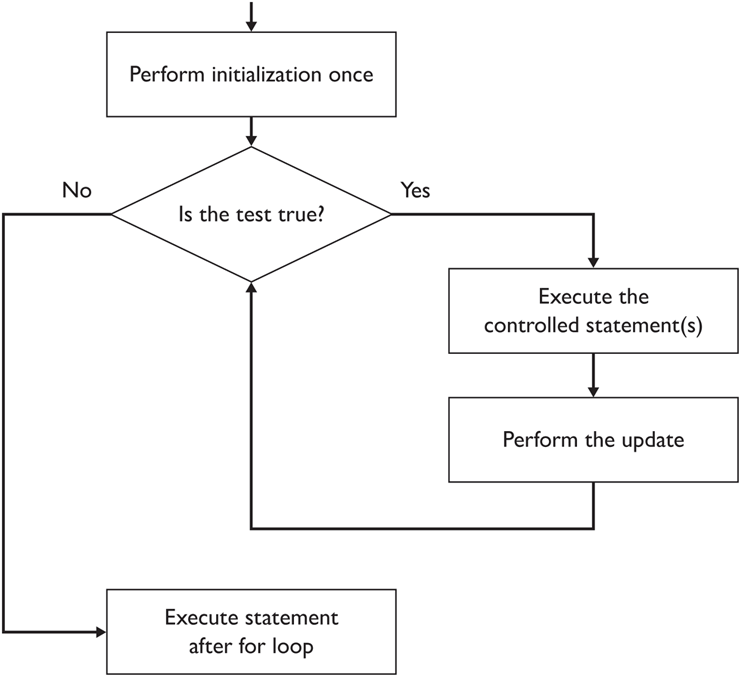
\includegraphics[width=\maxwidth,height=\maxheight,keepaspectratio,alt={Image}]{Figures/img_p69_0.png}}
\end{center}


\caption{Image}
\end{figure}

được thực hiện sau khi các câu lệnh được điều khiển đã được thực thi.
Khi phép kiểm tra đánh giá thành \texttt{false}, Java hoàn thành việc
thực thi vòng lặp và chuyển sang bất kỳ câu lệnh nào đứng sau vòng lặp.

Vòng lặp \texttt{for} là ví dụ đầu tiên về một cấu trúc điều khiển mà
chúng ta sẽ nghiên cứu.

\begin{quote}
\textbf{Cấu trúc điều khiển (Control Structure)} Một cấu trúc cú pháp
điều khiển các câu lệnh khác.
\end{quote}

Bạn nên cẩn thận sử dụng việc thụt lề để chỉ định các câu lệnh được điều
khiển. Trong trường hợp vòng lặp \texttt{for}, tất cả các câu lệnh trong
phần thân của vòng lặp được thụt lề như một cách để chỉ ra rằng chúng
nằm ``bên trong'' vòng lặp.

\subsubsection{\texorpdfstring{Theo Dõi Vòng Lặp \texttt{for} (Tracing
for
Loops)}{Theo Dõi Vòng Lặp for (Tracing for Loops)}}\label{theo-duxf5i-vuxf2ng-lux1eb7p-for-tracing-for-loops}

Hãy kiểm tra chi tiết vòng lặp \texttt{for} của chương trình
\texttt{WriteSquares2}:

\begin{verbatim}
for (int i = 1; i <= 5; i++) {
    System.out.println(i + " squared = " + (i * i));
}
\end{verbatim}

Trong vòng lặp này, phần khởi tạo (\texttt{int\ i\ =\ 1}) khai báo một
biến số nguyên \texttt{i} được khởi tạo bằng \texttt{1}. Phép kiểm tra
tiếp tục (\texttt{i\ \textless{}=\ 5}) chỉ ra rằng chúng ta nên tiếp tục
thực thi chừng nào \texttt{i} còn nhỏ hơn hoặc bằng \texttt{5}. Điều đó
có nghĩa là một khi \texttt{i} lớn hơn \texttt{5}, chúng ta sẽ dừng việc
thực thi phần thân của vòng lặp. Phần cập nhật (\texttt{i++}) sẽ tăng
giá trị của \texttt{i} thêm một mỗi lần, đưa \texttt{i} đến gần hơn với
việc lớn hơn \texttt{5}. Sau năm lần thực thi phần thân và năm lần cập
nhật đi kèm, \texttt{i} sẽ lớn hơn \texttt{5} và vòng lặp sẽ kết thúc
việc thực thi. Hình 2.2 theo dõi quá trình này một cách chi tiết.

\emph{Hình 2.2 Theo dõi chi tiết của vòng lặp \texttt{for}}

Java cho phép sự linh hoạt tuyệt vời trong việc quyết định những gì sẽ
đưa vào phần khởi tạo và phần cập nhật, vì vậy chúng ta có thể sử dụng
vòng lặp \texttt{for} để giải quyết đủ loại nhiệm vụ lập trình. Tuy
nhiên, hiện tại, chúng ta sẽ giới hạn mình trong một loại vòng lặp cụ
thể chuyên khai báo và khởi tạo một biến duy nhất được sử dụng để điều
khiển vòng lặp. Biến này thường được gọi là biến vòng lặp (loop
variable) của vòng lặp. Trong phần kiểm tra, chúng ta so sánh biến vòng
lặp với một số giá trị mong muốn cuối cùng, và trong phần cập nhật,
chúng ta thay đổi giá trị của biến vòng lặp, thường là tăng nó thêm
\texttt{1}. Các vòng lặp như vậy rất phổ biến trong lập trình. Theo quy
ước, chúng ta thường sử dụng các tên như \texttt{i}, \texttt{j}, và
\texttt{k} cho các biến vòng lặp.

\begin{figure}
\centering


\begin{center}
\pandocbounded{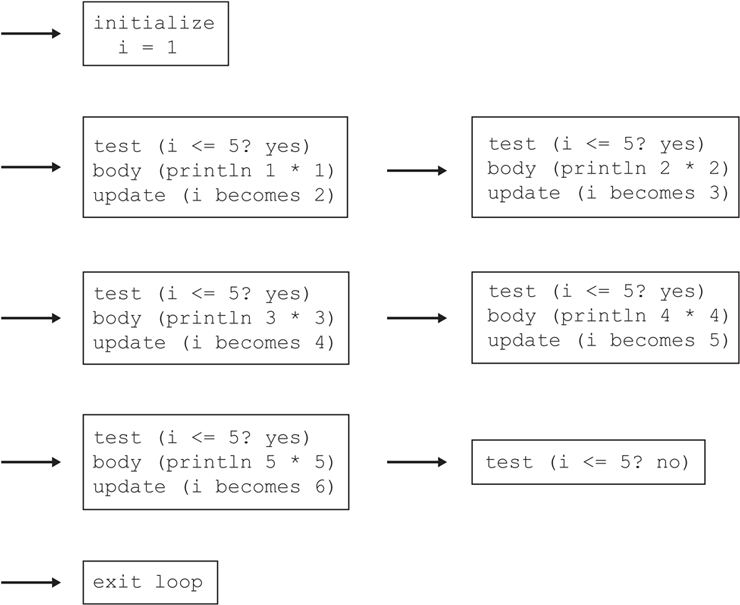
\includegraphics[width=\maxwidth,height=\maxheight,keepaspectratio,alt={Image}]{Figures/img_p72_0.png}}
\end{center}


\caption{Image}
\end{figure}

Mỗi lần thực thi câu lệnh được điều khiển của một vòng lặp được gọi là
một vòng lặp (iteration) của vòng lặp (như trong câu, ``Vòng lặp kết
thúc việc thực thi sau bốn vòng lặp''). Iteration (sự lặp lại) cũng dùng
để chỉ việc lặp nói chung (như trong câu, ``Tôi đã giải quyết bài toán
bằng cách sử dụng iteration'').

Hãy xem xét một vòng lặp \texttt{for} khác:

\begin{verbatim}
for (int i = -100; i <= 100; i++) {
    System.out.println(i + " squared = " + (i * i));
}
\end{verbatim}

Vòng lặp này thực thi tổng cộng \texttt{201} lần, tạo ra bình phương của
tất cả các số nguyên nằm giữa \texttt{-100} và \texttt{+100} bao gồm cả
hai đầu. Do đó, các giá trị được sử dụng trong phần khởi tạo và phần
kiểm tra có thể là bất kỳ số nguyên nào. Trên thực tế, chúng có thể là
các biểu thức số nguyên tùy ý:

\begin{verbatim}
for (int i = (2 + 2); i <= (17 * 3); i++) {
    System.out.println(i + " squared = " + (i * i));
}
\end{verbatim}

Vòng lặp này sẽ tạo ra bình phương của tất cả các số nguyên nằm giữa
\texttt{4} và \texttt{51} bao gồm cả hai đầu. Các dấu ngoặc đơn xung
quanh các biểu thức là không cần thiết nhưng cải thiện khả năng đọc. Hãy
xem xét vòng lặp sau:

\begin{verbatim}
for (int i = 1; i <= 30; i++) {
    System.out.println("+--------+");
}
\end{verbatim}

Vòng lặp này tạo ra \texttt{30} dòng kết quả đầu ra, tất cả đều hoàn
toàn giống nhau. Nó hơi khác so với vòng lặp trước bởi vì câu lệnh được
điều khiển bởi vòng lặp \texttt{for} không liên quan gì đến biến vòng
lặp. Do đó,

\begin{verbatim}
for (int i = -30; i <= -1; i++) {
    System.out.println("+--------+");
}
\end{verbatim}

tạo ra kết quả hoàn toàn giống y hệt. Hành vi của một vòng lặp như vậy
được xác định duy nhất bởi số vòng lặp (iterations) mà nó thực hiện. Số
vòng lặp được cung cấp bởi công thức:
\texttt{\textless{}giá\ trị\ kết\ thúc\textgreater{}\ -\ \textless{}giá\ trị\ bắt\ đầu\textgreater{}\ +\ 1}

Sẽ đơn giản hơn nhiều khi thấy rằng vòng lặp đầu tiên trong số này lặp
\texttt{30} lần, vì vậy tốt hơn là sử dụng vòng lặp đó.

Bây giờ chúng ta hãy xem xét một số trường hợp ranh giới (borderline
cases). Hãy xem xét vòng lặp này:

\begin{verbatim}
for (int i = 1; i <= 1; i++) {
    System.out.println("+--------+");
}
\end{verbatim}

Theo quy tắc của chúng ta, nó sẽ lặp một lần, và thực tế là như vậy. Nó
khởi tạo biến \texttt{i} bằng \texttt{1} và kiểm tra xem biến này có nhỏ
hơn hoặc bằng \texttt{1} hay không, và điều đó là đúng. Vì vậy, nó thực
thi \texttt{println}, tăng \texttt{i}, và kiểm tra lại. Lần thứ hai nó
kiểm tra, nó thấy rằng \texttt{i} không còn nhỏ hơn hoặc bằng \texttt{1}
nữa, vì vậy nó ngừng thực thi. Bây giờ hãy xem xét vòng lặp này:

\begin{verbatim}
for (int i = 1; i <= 0; i++) {
    System.out.println("+--------+"); // never executes
}
\end{verbatim}

Vòng lặp này hoàn toàn không thực hiện vòng lặp nào cả. Nó sẽ không gây
ra lỗi thực thi; nó chỉ là không thực thi phần thân. Nó khởi tạo biến
thành \texttt{1} và kiểm tra xem biến này có nhỏ hơn hoặc bằng
\texttt{0} hay không. Điều đó là sai, vì vậy thay vì thực thi các câu
lệnh trong phần thân, nó dừng lại ngay ở đó.

Khi bạn xây dựng một vòng lặp \texttt{for}, bạn có thể đưa vào nhiều hơn
một câu lệnh bên trong các dấu ngoặc nhọn. Chẳng hạn, hãy xem xét đoạn
mã sau:

\begin{verbatim}
for (int i = 1; i <= 20; i++) {
    System.out.println("Hi!");
    System.out.println("Ho!");
}
\end{verbatim}

Đoạn mã này sẽ tạo ra \texttt{20} cặp dòng, dòng đầu tiên có từ ``Hi!''
trên đó và dòng thứ hai có từ ``Ho!''.

Khi một vòng lặp \texttt{for} điều khiển một câu lệnh duy nhất, bạn
không bắt buộc phải bao gồm các dấu ngoặc nhọn. Các dấu ngoặc nhọn chỉ
được yêu cầu đối với các tình huống như tình huống trước, nơi bạn có
nhiều hơn một câu lệnh mà bạn muốn vòng lặp điều khiển. Tuy nhiên, quy
ước viết mã của Java là luôn bao gồm các dấu ngoặc nhọn ngay cả đối với
một câu lệnh duy nhất, và chúng tôi tuân theo quy ước này trong cuốn
sách này. Có hai ưu điểm đối với quy ước này: - Việc bao gồm các dấu
ngoặc nhọn ngăn ngừa các lỗi trong tương lai. Ngay cả khi bây giờ bạn
chỉ cần một câu lệnh trong phần thân của vòng lặp, mã của bạn có thể sẽ
thay đổi theo thời gian. Việc có sẵn các dấu ngoặc nhọn ở đó đảm bảo
rằng, nếu bạn thêm một câu lệnh bổ sung vào phần thân sau này, bạn sẽ
không vô tình quên bao gồm chúng. Nói chung, việc bao gồm các dấu ngoặc
nhọn trước sẽ đỡ tốn công sức hơn so với việc phải tìm kiếm các lỗi khó
hiểu sau này. - Luôn bao gồm các dấu ngoặc nhọn làm giảm mức độ chi tiết
bạn phải xem xét khi học các cấu trúc điều khiển mới. Sẽ mất thời gian
để làm chủ các chi tiết của bất kỳ cấu trúc điều khiển mới nào, và việc
làm chủ những chi tiết đó sẽ dễ dàng hơn nếu bạn không phải suy nghĩ
thêm về việc khi nào nên bao gồm và khi nào không nên bao gồm các dấu
ngoặc.

\begin{quote}
{[}!WARNING{]} \textbf{LỖI LẬP TRÌNH PHỔ BIẾN} \textbf{Quên Dấu Ngoặc
Nhọn (Forgetting Curly Braces)}

Bạn nên sử dụng việc thụt lề để chỉ định phần thân của một vòng lặp
\texttt{for}, nhưng thụt lề thôi là chưa đủ. Java bỏ qua việc thụt lề
khi quyết định xem các câu lệnh khác nhau được nhóm lại như thế nào.
Chẳng hạn, giả sử bạn viết đoạn mã sau:

\begin{verbatim}
for (int i = 1; i <= 20; i++)
    System.out.println("Hi!");
    System.out.println("Ho!");
\end{verbatim}

Việc thụt lề chỉ ra cho người đọc rằng cả hai câu lệnh \texttt{println}
đều nằm trong phần thân của vòng lặp \texttt{for}, nhưng không có bất kỳ
dấu ngoặc nhọn nào để báo cho Java biết điều đó. Kết quả là, đoạn mã này
được diễn giải như sau:

\begin{verbatim}
for (int i = 1; i <= 20; i++) {
    System.out.println("Hi!");
}
System.out.println("Ho!");
\end{verbatim}

Chỉ câu lệnh \texttt{println} đầu tiên được coi là nằm trong phần thân
của vòng lặp \texttt{for}. Câu lệnh \texttt{println} thứ hai được coi là
nằm bên ngoài vòng lặp. Vì vậy, đoạn mã này sẽ tạo ra \texttt{20} dòng
kết quả đầu ra đều ghi là ``Hi!'' theo sau là một dòng kết quả đầu ra
ghi là ``Ho!''. Để bao gồm cả hai lệnh \texttt{println} vào trong phần
thân, bạn cần các dấu ngoặc nhọn xung quanh chúng:

\begin{verbatim}
for (int i = 1; i <= 20; i++) {
    System.out.println("Hi!");
    System.out.println("Ho!");
}
\end{verbatim}
\end{quote}

\subsubsection{\texorpdfstring{Các Mẫu Vòng Lặp \texttt{for} (for Loop
Patterns)}{Các Mẫu Vòng Lặp for (for Loop Patterns)}}\label{cuxe1c-mux1eabu-vuxf2ng-lux1eb7p-for-for-loop-patterns}

Nói chung, nếu bạn muốn một vòng lặp thực hiện chính xác \(n\) lần lặp,
bạn sẽ sử dụng một trong hai vòng lặp tiêu chuẩn. Dạng tiêu chuẩn đầu
tiên trông giống như những dạng bạn đã thấy:

\begin{verbatim}
for (int <variable> = 1; <variable> <= n; <variable>++) {
    <statement>;
    <statement>;
    ...
    <statement>;
}
\end{verbatim}

Khá rõ ràng là vòng lặp này thực thi \(n\) lần, bởi vì nó bắt đầu ở
\texttt{1} và tiếp tục chừng nào nó còn nhỏ hơn hoặc bằng \(n\). Ví dụ,
vòng lặp này in ra các số từ \texttt{1} đến \texttt{10}:

\begin{verbatim}
for (int i = 1; i <= 10; i++) {
    System.out.print(i + " ");
}
\end{verbatim}

Bởi vì nó sử dụng một câu lệnh \texttt{print} thay vì \texttt{println},
nó tạo ra một dòng kết quả đầu ra duy nhất:

\begin{verbatim}
1 2 3 4 5 6 7 8 9 10
\end{verbatim}

Tuy nhiên, thường thì việc bắt đầu đếm của chúng ta ở số \texttt{0} thay
vì \texttt{1} sẽ thuận tiện hơn. Điều đó đòi hỏi phải có sự thay đổi
trong phần kiểm tra vòng lặp để cho phép bạn dừng lại khi nó nhỏ hơn
\(n\) một đơn vị:

\begin{verbatim}
for (int <variable> = 0; <variable> < n; i++) {
    <statement>;
    <statement>;
    ...
    <statement>;
}
\end{verbatim}

Lưu ý rằng trong dạng này, khi bạn khởi tạo biến thành \texttt{0}, bạn
kiểm tra xem nó có nhỏ hơn một cách nghiêm ngặt so với \(n\) hay không.
Cả hai dạng sẽ thực thi chính xác \(n\) lần, mặc dù có một số tình huống
mà vòng lặp dựa trên số không (zero-based loop) hoạt động tốt hơn. Ví
dụ, vòng lặp này thực thi \texttt{10} lần giống như vòng lặp trước:

\begin{verbatim}
for (int i = 0; i < 10; i++) {
    System.out.print(i + " ");
}
\end{verbatim}

Bởi vì nó bắt đầu ở \texttt{0} thay vì bắt đầu ở \texttt{1}, nó tạo ra
một chuỗi \texttt{10} giá trị khác nhau:

\begin{verbatim}
0 1 2 3 4 5 6 7 8 9
\end{verbatim}

Thông thường nhất, bạn sẽ sử dụng vòng lặp bắt đầu ở \texttt{0} hoặc
\texttt{1} để thực hiện một số thao tác một số lần cố định. Nhưng có một
biến thể nhỏ đôi khi cũng hữu ích. Thay vì chạy vòng lặp theo hướng
tiến, chúng ta có thể chạy nó theo hướng lùi. Thay vì bắt đầu ở
\texttt{1} và thực thi cho đến khi bạn đạt đến \(n\), bạn lại bắt đầu ở
\(n\) và tiếp tục thực thi cho đến khi bạn đạt đến \texttt{1}. Bạn có
thể đạt được điều này bằng cách sử dụng phép giảm (decrement) thay vì
phép tăng (increment), vì vậy đôi khi chúng ta gọi đây là một vòng lặp
giảm (decrementing loop).

Dưới đây là dạng tổng quát của một vòng lặp giảm:

\begin{verbatim}
for (int <variable> = n; <variable> >= 1; <variable>--) {
    <statement>;
    <statement>;
    ...
    <statement>;
}
\end{verbatim}

Ví dụ, dưới đây là một vòng lặp giảm thực thi \texttt{10} lần:

\begin{verbatim}
for (int i = 10; i >= 1; i--) {
    System.out.print(i + " ");
}
\end{verbatim}

Bởi vì nó chạy lùi, nó in ra các giá trị theo thứ tự ngược lại:

\begin{verbatim}
10 9 8 7 6 5 4 3 2 1
\end{verbatim}

JShell cho phép bạn viết các vòng lặp \texttt{for}. Vì một vòng lặp kéo
dài nhiều dòng, shell sẽ hiển thị lời nhắc tiếp tục là
\texttt{...\textgreater{}} trên mỗi dòng tiếp theo cho đến khi bạn kết
thúc vòng lặp bằng cách viết dấu ngoặc nhọn đóng \texttt{\}}, như được
hiển thị trong tương tác sau. Khi bạn viết xong vòng lặp hoàn chỉnh,
vòng lặp sẽ thực thi.

\begin{verbatim}
jshell> for (int i = 1; i <= 10; i++) {
  ...>     System.out.print(i + "! ");
  ...> } 
1! 2! 3! 4! 5! 6! 7! 8! 9! 10!
\end{verbatim}

\subsubsection{\texorpdfstring{Các Vòng Lặp \texttt{for} Lồng Nhau
(Nested for
Loops)}{Các Vòng Lặp for Lồng Nhau (Nested for Loops)}}\label{cuxe1c-vuxf2ng-lux1eb7p-for-lux1ed3ng-nhau-nested-for-loops}

Vòng lặp \texttt{for} điều khiển một câu lệnh, và bản thân vòng lặp
\texttt{for} cũng là một câu lệnh, điều đó có nghĩa là một vòng lặp
\texttt{for} có thể điều khiển một vòng lặp \texttt{for} khác. Ví dụ,
bạn có thể viết đoạn mã như sau:

\begin{verbatim}
for (int i = 1; i <= 10; i++) {
    for (int j = 1; j <= 5; j++) {
        System.out.println("Hi there.");
    }
}
\end{verbatim}

Đoạn mã này có lẽ dễ đọc hơn từ trong ra ngoài. Câu lệnh
\texttt{println} tạo ra một dòng kết quả đầu ra duy nhất. Vòng lặp
\texttt{j} bên trong thực thi câu lệnh này năm lần, tạo ra năm dòng kết
quả đầu ra. Vòng lặp \texttt{i} bên ngoài thực thi vòng lặp bên trong
\texttt{10} lần, tạo ra \texttt{10} tập hợp gồm \texttt{5} dòng, hay
\texttt{50} dòng kết quả đầu ra. Do đó, đoạn mã trước đó tương đương
với:

\begin{verbatim}
for (int i = 1; i <= 50; i++) {
    System.out.println("Hi there.");
}
\end{verbatim}

Ví dụ này cho thấy rằng một vòng lặp \texttt{for} có thể được điều khiển
bởi một vòng lặp \texttt{for} khác. Một vòng lặp như vậy được gọi là một
vòng lặp lồng nhau (nested loop). Tuy nhiên, ví dụ này không thú vị lắm,
bởi vì vòng lặp lồng nhau có thể bị loại bỏ.

Bây giờ bạn đã biết cách viết các vòng lặp \texttt{for}, bạn sẽ muốn có
thể tạo ra các dòng kết quả đầu ra phức tạp từng phần một bằng cách sử
dụng lệnh \texttt{print}. Hãy nhớ lại từ Chương 1 rằng lệnh
\texttt{print} in trên dòng kết quả đầu ra hiện tại mà không chuyển sang
dòng kết quả đầu ra mới. Ví dụ, nếu bạn muốn tạo ra một dòng kết quả đầu
ra có \texttt{80} ngôi sao trên đó, bạn có thể sử dụng một lệnh
\texttt{print} để in từng ngôi sao một và để nó thực thi \texttt{80} lần
thay vì sử dụng một lệnh \texttt{println} duy nhất.

Hãy xem xét một vòng lặp lồng nhau thú vị hơn sử dụng lệnh
\texttt{print}:

\begin{verbatim}
for (int i = 1; i <= 6; i++) {
    for (int j = 1; j <= 3; j++) {
        System.out.print(j + " ");
    }
}
\end{verbatim}

Chúng ta có thể một lần nữa đọc điều này từ trong ra ngoài. Vòng lặp bên
trong in ra giá trị của biến vòng lặp \texttt{j} của nó khi nó thay đổi
từ \texttt{1} đến \texttt{3}. Vòng lặp bên ngoài thực thi điều này sáu
lần khác nhau. Kết quả là, chúng ta nhận được sáu lần xuất hiện của
chuỗi \texttt{1\ 2\ 3} làm kết quả đầu ra:

\begin{verbatim}
1 2 3 1 2 3 1 2 3 1 2 3 1 2 3 1 2 3
\end{verbatim}

Đoạn mã này in tất cả kết quả đầu ra của nó trên một dòng kết quả đầu ra
duy nhất. Hãy xem một số mã bao gồm sự kết hợp của \texttt{print} và
\texttt{println} để tạo ra một số dòng kết quả đầu ra:

\begin{verbatim}
for (int i = 1; i <= 6; i++) {
    for (int j = 1; j <= 10; j++) {
        System.out.print("*");
    }
    System.out.println();
}
\end{verbatim}

Khi bạn viết đoạn mã có liên quan đến các vòng lặp lồng nhau, bạn phải
cẩn thận thụt lề đoạn mã một cách chính xác để làm cho cấu trúc rõ ràng.
Ở cấp độ ngoài cùng, đoạn mã trước đó là một vòng lặp \texttt{for} đơn
giản thực thi sáu lần:

\begin{verbatim}
for (int i = 1; i <= 6; i++) {
    ...
}
\end{verbatim}

Chúng ta sử dụng thụt lề cho các câu lệnh bên trong vòng lặp
\texttt{for} này để làm rõ rằng chúng là phần thân của vòng lặp này. Bên
trong, chúng ta tìm thấy hai câu lệnh: một vòng lặp \texttt{for} khác và
một \texttt{println}. Hãy xem xét vòng lặp \texttt{for} bên trong:

\begin{verbatim}
for (int j = 1; j <= 10; j++) {
    System.out.print("*");
}
\end{verbatim}

Vòng lặp này được điều khiển bởi vòng lặp \texttt{for} bên ngoài, đó là
lý do tại sao nó được thụt lề, nhưng bản thân nó lại điều khiển một câu
lệnh (câu lệnh \texttt{print}), vì vậy chúng ta lại có thêm một cấp độ
thụt lề nữa. Do đó, việc thụt lề chỉ ra rằng câu lệnh \texttt{print}
được điều khiển bởi vòng lặp \texttt{for} bên trong, và vòng lặp này đến
lượt nó lại được điều khiển bởi vòng lặp \texttt{for} bên ngoài. Vậy
vòng lặp bên trong này làm gì? Nó in ra \texttt{10} ngôi sao trên dòng
kết quả đầu ra hiện tại. Chúng đều xuất hiện trên cùng một dòng vì chúng
ta đang sử dụng một lệnh \texttt{print} thay vì \texttt{println}. Lưu ý
rằng sau vòng lặp này, chúng ta thực hiện một lệnh \texttt{println}:

\begin{verbatim}
System.out.println();
\end{verbatim}

Hiệu ứng ròng của vòng lặp \texttt{for} theo sau bởi \texttt{println} là
chúng ta nhận được một dòng kết quả đầu ra với \texttt{10} ngôi sao trên
đó. Nhưng hãy nhớ rằng các câu lệnh này được chứa trong một vòng lặp bên
ngoài thực thi sáu lần, vì vậy cuối cùng chúng ta nhận được sáu dòng kết
quả đầu ra, mỗi dòng có \texttt{10} ngôi sao:

\begin{verbatim}
********** 
********** 
********** 
********** 
********** 
**********
\end{verbatim}

Hãy xem xét thêm một biến thể nữa. Trong đoạn mã trên, vòng lặp
\texttt{for} bên trong luôn thực hiện chính xác một công việc giống
nhau: Nó in chính xác \texttt{10} ngôi sao trên một dòng kết quả đầu ra.
Nhưng điều gì sẽ xảy ra nếu chúng ta thay đổi phép kiểm tra cho vòng lặp
\texttt{for} bên trong để sử dụng biến (\texttt{i}) của vòng lặp
\texttt{for} bên ngoài?

\begin{verbatim}
for (int i = 1; i <= 6; i++) {
    for (int j = 1; j <= i; j++) {
        System.out.print("*");
    }
    System.out.println();
}
\end{verbatim}

Trong phiên bản cũ, vòng lặp bên trong luôn thực thi \texttt{10} lần,
tạo ra \texttt{10} ngôi sao trên mỗi dòng kết quả đầu ra. Với phép kiểm
tra mới (\texttt{j\ \textless{}=\ i}), vòng lặp bên trong sẽ thực thi
\texttt{i} lần với mỗi lần lặp. Nhưng \texttt{i} đang thay đổi: Nó nhận
các giá trị \texttt{1}, \texttt{2}, \texttt{3}, \texttt{4}, \texttt{5},
và \texttt{6}. Ở lần lặp đầu tiên của vòng lặp bên ngoài, khi \texttt{i}
là \texttt{1}, phép kiểm tra \texttt{j\ \textless{}=\ i} thực chất là
đang kiểm tra \texttt{j\ \textless{}=\ 1}, và nó tạo ra một dòng có một
ngôi sao trên đó. Ở lần lặp thứ hai của vòng lặp bên ngoài, khi
\texttt{i} là \texttt{2}, phép kiểm tra thực chất là đang kiểm tra
\texttt{j\ \textless{}=\ 2}, và nó tạo ra một dòng có hai ngôi sao trên
đó. Ở lần lặp thứ ba của vòng lặp bên ngoài, khi \texttt{i} là
\texttt{3}, phép kiểm tra thực chất là đang kiểm tra
\texttt{j\ \textless{}=\ 3}, và nó tạo ra một dòng có ba ngôi sao trên
đó. Quá trình này tiếp tục qua lần lặp thứ sáu.

Nói cách khác, đoạn mã này tạo ra một hình tam giác làm kết quả đầu ra:

\begin{verbatim}
* 
** 
*** 
**** 
***** 
******
\end{verbatim}

\subsection{Quản Lý Độ Phức Tạp (Managing
Complexity)}\label{quux1ea3n-luxfd-ux111ux1ed9-phux1ee9c-tux1ea1p-managing-complexity}

Bạn đã học về một số cấu trúc lập trình mới trong chương này, và đã đến
lúc kết hợp các mảnh ghép lại với nhau để giải quyết một số nhiệm vụ
phức tạp. Như chúng tôi đã chỉ ra trong Chương 1, Brian Kernighan, một
trong những đồng tác giả của cuốn \emph{The C Programming Language}, đã
nói rằng ``Kiểm soát độ phức tạp là bản chất của lập trình máy tính''
(``Controlling complexity is the essence of computer programming'').
Trong phần này, chúng ta sẽ xem xét một số kỹ thuật mà các nhà khoa học
máy tính sử dụng để giải quyết các vấn đề phức tạp mà không bị choáng
ngợp bởi độ phức tạp.

\subsubsection{Phạm Vi (Scope)}\label{phux1ea1m-vi-scope}

Khi các chương trình trở nên dài hơn, khả năng các phần khác nhau của
chương trình can thiệp lẫn nhau ngày càng tăng. Java giúp chúng ta quản
lý vấn đề tiềm ẩn này bằng cách thực thi các quy tắc về phạm vi.

\begin{quote}
\textbf{Phạm vi (Scope)} Phần của một chương trình mà tại đó một khai
báo cụ thể có giá trị hợp lệ.
\end{quote}

Như bạn đã thấy, khi nói đến việc khai báo các phương thức tĩnh (static
methods), bạn có thể đặt chúng theo bất kỳ thứ tự nào. Phạm vi của một
phương thức tĩnh là toàn bộ lớp mà nó xuất hiện. Các biến lại hoạt động
khác. Quy tắc đơn giản là phạm vi của một khai báo biến mở rộng từ điểm
mà nó được khai báo đến dấu ngoặc nhọn đóng \texttt{\}} bao bọc nó. Nói
cách khác, hãy tìm cặp dấu ngoặc nhọn trực tiếp bao bọc khai báo biến.
Phạm vi của biến là từ điểm nó được khai báo đến dấu ngoặc nhọn đóng.

Quy tắc phạm vi này có một số hàm ý. Đầu tiên, hãy xem xét nó có ý nghĩa
gì đối với các phương thức khác nhau. Mỗi phương thức có tập hợp các dấu
ngoặc nhọn riêng để chỉ định các câu lệnh sẽ được thực thi khi phương
thức được gọi. Bất kỳ biến nào được khai báo bên trong các dấu ngoặc
nhọn của một phương thức sẽ không có sẵn ở bên ngoài phương thức đó.
Chúng ta gọi các biến như vậy là các biến cục bộ (local variables), và
chúng ta gọi quá trình giới hạn phạm vi của chúng là cục bộ hóa các biến
(localizing variables).

\begin{quote}
\textbf{Biến cục bộ (Local Variable)} Một biến được khai báo bên trong
một phương thức, chỉ có thể truy cập được trong phương thức đó.
\end{quote}

\begin{quote}
\textbf{Cục bộ hóa các biến (Localizing Variables)} Khai báo các biến
trong phạm vi cục bộ nhất (trong cùng nhất) có thể.
\end{quote}

Nói chung, bạn sẽ muốn khai báo các biến trong phạm vi cục bộ nhất có
thể. Bạn có thể tự hỏi tại sao chúng ta lại muốn cục bộ hóa các biến chỉ
trong một phương thức. Tại sao không khai báo tất cả mọi thứ trong một
phạm vi bên ngoài duy nhất? Điều đó chắc chắn có vẻ đơn giản hơn, nhưng
có một số nhược điểm quan trọng. Việc cục bộ hóa các biến dẫn đến một số
sự trùng lặp (và có thể gây nhầm lẫn) nhưng cung cấp bảo mật tốt hơn. Để
so sánh, hãy xem xét việc sử dụng tủ lạnh trong các ký túc xá. Mỗi phòng
ký túc xá có thể có tủ lạnh riêng, nhưng nếu bạn ở bên ngoài một phòng,
bạn không biết liệu nó có tủ lạnh bên trong hay không. Nội dung của căn
phòng được giấu kín khỏi bạn.

Các chương trình Java sử dụng các biến để lưu trữ các giá trị giống như
sinh viên sử dụng tủ lạnh để lưu trữ bia, kem và những thứ có giá trị
khác. Lần cuối cùng chúng tôi ở trong một ký túc xá, chúng tôi nhận thấy
rằng hầu hết các phòng cá nhân đều có tủ lạnh bên trong. Điều này có vẻ
cực kỳ dư thừa, nhưng lý do thì quá rõ ràng. Nếu bạn muốn đảm bảo an
toàn cho một thứ gì đó, bạn đặt nó ở nơi mà không ai khác có thể lấy
được. Bạn sẽ sử dụng các biến cục bộ trong các chương trình của mình
theo cách rất giống như vậy. Nếu mỗi phương thức riêng lẻ có các biến
cục bộ riêng để sử dụng, bạn không phải xem xét khả năng can thiệp từ
các phần khác của chương trình.

Hãy xem xét một ví dụ đơn giản liên quan đến hai phương thức:

\begin{verbatim}
 1  // This program does not compile.
 2  public class ScopeExample {
 3      public static void main(String[] args) {
 4          int x = 3;
 5          int y = 7;
 6          computeSum();
 7      }
 8
 9      public static void computeSum() {
10          int sum = x + y; // illegal, x/y are not in scope
11          System.out.println("sum = " + sum);
12      }
13  }
\end{verbatim}

Trong ví dụ này, phương thức \texttt{main} khai báo các biến cục bộ
\texttt{x} và \texttt{y} và cung cấp cho chúng các giá trị khởi tạo. Sau
đó, nó gọi phương thức \texttt{computeSum}. Bên trong phương thức này,
chúng ta cố gắng sử dụng các giá trị của \texttt{x} và \texttt{y} để
tính tổng. Tuy nhiên, vì các biến \texttt{x} và \texttt{y} là cục bộ đối
với phương thức \texttt{main} và không hiển thị bên trong phương thức
\texttt{computeSum}, điều này không hoạt động. (Trong chương tiếp theo,
chúng ta sẽ thấy một kỹ thuật cho phép một phương thức truyền một giá
trị cho phương thức khác.)

Chương trình tạo ra các thông báo lỗi giống như sau:

\begin{verbatim}
ScopeExample.java:10: error: cannot find symbol
symbol  : variable x
location: class ScopeExample
        int sum = x + y;  // illegal, x/y are not in scope
                  ^
ScopeExample.java:10: error: cannot find symbol
symbol  : variable y
location: class ScopeExample
        int sum = x + y;  // illegal, x/y are not in scope
                      ^
\end{verbatim}

Việc hiểu phạm vi trong việc thảo luận về các biến cục bộ của phương
thức này so với phương thức khác là rất quan trọng. Phạm vi cũng có hàm
ý đối với những gì xảy ra bên trong một phương thức duy nhất. Bạn đã
thấy rằng các dấu ngoặc nhọn được sử dụng để nhóm một loạt các câu lệnh
lại với nhau. Nhưng bạn có thể có các dấu ngoặc nhọn bên trong các dấu
ngoặc nhọn, và điều này dẫn đến một số vấn đề về phạm vi. Ví dụ, hãy xem
xét đoạn mã sau:

\begin{verbatim}
for (int i = 1; i <= 5; i++) {
    int squared = i * i;
    System.out.println(i + " squared = " + squared);
}
\end{verbatim}

Đây là một biến thể của đoạn mã mà chúng ta đã xem xét trước đó trong
chương để in ra bình phương của năm số nguyên đầu tiên. Trong phiên bản
này, một biến được gọi là \texttt{squared} được sử dụng để theo dõi bình
phương của biến vòng lặp \texttt{for}. Đoạn mã này hoạt động tốt, nhưng
hãy xem xét biến thể này:

\begin{verbatim}
for (int i = 1; i <= 5; i++) {
    int squared = i * i;
    System.out.println(i + " squared = " + squared);
}
System.out.println("Last square = " + squared); // illegal
\end{verbatim}

Đoạn mã này tạo ra một lỗi trình biên dịch. Biến \texttt{squared} được
khai báo bên trong vòng lặp \texttt{for}. Nói cách khác, các dấu ngoặc
nhọn chứa nó là các dấu ngoặc nhọn của vòng lặp. Nó không thể được sử
dụng bên ngoài phạm vi này, vì vậy khi bạn cố gắng tham chiếu đến nó bên
ngoài vòng lặp, bạn sẽ nhận được lỗi biên dịch.

Nếu vì lý do nào đó bạn cần viết mã như thế này để truy cập biến sau
vòng lặp, bạn phải khai báo biến trong phạm vi bên ngoài, trước vòng
lặp:

\begin{verbatim}
int squared = 0;   // declaration is now in outer scope
for (int i = 1; i <= 5; i++) {
    squared = i * i;   // change this to an assignment statement
    System.out.println(i + " squared = " + squared);
}
System.out.println("Last square = " + squared); // now legal
\end{verbatim}

Có một vài trường hợp đặc biệt đối với phạm vi, và vòng lặp \texttt{for}
là một trong số đó. Khi một biến được khai báo trong phần khởi tạo của
một vòng lặp \texttt{for}, phạm vi của nó chỉ là bản thân vòng lặp
\texttt{for} (ba phần trong tiêu đề vòng lặp \texttt{for} và các câu
lệnh được điều khiển bởi vòng lặp \texttt{for}). Điều đó có nghĩa là bạn
có thể sử dụng cùng một tên biến trong nhiều vòng lặp \texttt{for}:

\begin{verbatim}
for (int i = 1; i <= 10; i++) {
    System.out.println(i + " squared = " + (i * i));
}
for (int i = 1; i <= 10; i++) {
    System.out.println(i + " cubed = " + (i * i * i));
}
\end{verbatim}

Biến \texttt{i} được khai báo hai lần trong đoạn mã trước đó, nhưng vì
phạm vi của mỗi biến chỉ là vòng lặp \texttt{for} mà nó được khai báo,
nên đây không phải là vấn đề. (Điều này giống như việc có hai phòng ký
túc xá, mỗi phòng đều có tủ lạnh riêng.) Tất nhiên, bạn không thể làm
điều này với các vòng lặp \texttt{for} lồng nhau. Chẳng hạn, đoạn mã sau
sẽ không biên dịch được:

\begin{verbatim}
for (int i = 1; i <= 5; i++) {
    for (int i = 1; i <= 10; i++) { // illegal
        System.out.println("hi there.");
    }
}
\end{verbatim}

Khi Java gặp vòng lặp \texttt{for} bên trong, nó sẽ phàn nàn rằng biến
\texttt{i} đã được khai báo trong phạm vi này. Bạn không thể khai báo
cùng một biến hai lần trong cùng một phạm vi. Bạn phải đưa ra hai tên
khác nhau để phân biệt chúng, giống như khi có hai người tên Carl trong
cùng một gia đình, họ có xu hướng được gọi là ``Carl con'' và ``Carl
bố'' để tránh bất kỳ sự nhầm lẫn tiềm ẩn nào.

Một biến vòng lặp được sử dụng trong vòng lặp \texttt{for} không nhất
thiết phải được khai báo trong phần khởi tạo của vòng lặp. Bạn có thể
tách việc khai báo biến vòng lặp \texttt{for} khỏi việc khởi tạo biến,
như trong đoạn mã sau:

\begin{verbatim}
int i;
for (i = 1; i <= 5; i++) {
    System.out.println(i + " squared = " + (i * i));
}
\end{verbatim}

Làm như vậy sẽ mở rộng phạm vi của biến đến cuối tập hợp dấu ngoặc nhọn
bao bọc. Một ưu điểm của phương pháp này là nó cho phép bạn tham chiếu
đến giá trị cuối cùng của biến vòng lặp sau vòng lặp. Thông thường bạn
sẽ không thể làm điều này, bởi vì phạm vi của biến vòng lặp sẽ bị giới
hạn ở chính vòng lặp đó. Tuy nhiên, việc khai báo biến vòng lặp bên
ngoài vòng lặp là một thói quen nguy hiểm, và nó cung cấp một ví dụ tốt
về các vấn đề bạn có thể gặp phải khi bạn không cục bộ hóa các biến.
Chẳng hạn, hãy xem xét đoạn mã sau:

\begin{verbatim}
int i;
for (i = 1; i <= 5; i++) {
    for (i = 1; i <= 10; i++) {
        System.out.println("hi there.");
    }
}
\end{verbatim}

Như đã lưu ý ở trên, bạn không nên sử dụng cùng một biến vòng lặp khi
bạn có các vòng lặp lồng nhau. Nhưng không giống như ví dụ trước, đoạn
mã này biên dịch được, bởi vì ở đây khai báo biến nằm ngoài vòng lặp
\texttt{for} bên ngoài. Vì vậy, thay vì nhận được một thông báo lỗi hữu
ích từ trình biên dịch Java, bạn nhận được một chương trình có lỗi (bug)
trong đó. Từ việc đọc các vòng lặp này, bạn có thể nghĩ rằng đoạn mã sẽ
tạo ra \texttt{50} dòng kết quả đầu ra, nhưng thực tế nó chỉ tạo ra
\texttt{10} dòng kết quả đầu ra. Vòng lặp bên trong tăng biến \texttt{i}
cho đến khi nó trở thành \texttt{11}, và điều đó khiến vòng lặp bên
ngoài chấm dứt chỉ sau một lần lặp. Sẽ còn tồi tệ hơn nếu bạn đảo ngược
thứ tự của các vòng lặp này:

\begin{verbatim}
int i;
for (i = 1; i <= 10; i++) {
    for (i = 1; i <= 5; i++) {
        System.out.println("hi there.");
    }
}
\end{verbatim}

Đoạn mã này có một vòng lặp vô hạn (infinite loop).

\begin{quote}
\textbf{Vòng lặp vô hạn (Infinite Loop)} Một vòng lặp không bao giờ kết
thúc.
\end{quote}

Vòng lặp này là vô hạn bởi vì bất kể vòng lặp bên ngoài làm gì với biến
\texttt{i}, vòng lặp bên trong luôn đặt nó trở lại \texttt{1} và lặp cho
đến khi nó trở thành \texttt{6}. Vòng lặp bên ngoài sau đó tăng biến lên
\texttt{7} và thấy rằng \texttt{7} nhỏ hơn hoặc bằng \texttt{10}, vì vậy
nó luôn quay trở lại vòng lặp bên trong, vòng lặp bên trong một lần nữa
lại đặt biến trở lại \texttt{1} và lặp cho đến \texttt{6}. Quá trình này
diễn ra vô tận. Đây là những loại vấn đề can thiệp mà bạn có thể gặp
phải khi không cục bộ hóa các biến.

\begin{quote}
{[}!WARNING{]} \textbf{LỖI LẬP TRÌNH PHỔ BIẾN} \textbf{Tham Chiếu Sai
Biến Vòng Lặp (Referring to the Wrong Loop Variable)}

Đoạn mã sau được dự định để in ra một hình tam giác các ngôi sao. Tuy
nhiên, nó có một lỗi tinh vi khiến nó in ra các ngôi sao vô hạn:

\begin{verbatim}
for (int i = 1; i <= 6; i++) {
    for (int j = 1; j <= i; i++){
        System.out.print("*");
    }
    System.out.println();
}
\end{verbatim}

Vấn đề nằm ở dòng thứ hai, trong câu lệnh cập nhật ở tiêu đề của vòng
lặp \texttt{for} bên trong. Lập trình viên định viết \texttt{j++} nhưng
thay vào đó lại vô tình viết \texttt{i++}. Một dấu vết của đoạn mã được
hiển thị trong Bảng 2.6.

\emph{Bảng 2.6 Dấu vết của vòng lặp \texttt{for} lồng nhau}

Biến \texttt{j} đáng lẽ ra phải tăng lên, nhưng thay vào đó \texttt{i}
lại tăng. Hậu quả của lỗi này là biến \texttt{j} không bao giờ được tăng
trong vòng lặp bên trong, và do đó phép kiểm tra
\texttt{j\ \textless{}=\ i} không bao giờ thất bại, vì vậy vòng lặp bên
trong không kết thúc. Dưới đây là một đoạn mã bị hỏng khác. Đoạn mã này
cố gắng in một hộp các ngôi sao kích thước \texttt{6\ x\ 4}, nhưng nó
cũng in vô hạn:

\begin{verbatim}
for (int i = 1; i <= 6; i++) {
    for (int j = 1; i <= 4; j++) {
        System.out.print("*");
    }
\end{verbatim}
\end{quote}

\begin{verbatim}
    System.out.println();
}
\end{verbatim}

Vấn đề nằm ở dòng thứ hai, lần này là trong phép kiểm tra ở tiêu đề của
vòng lặp \texttt{for} bên trong. Lập trình viên định viết
\texttt{j\ \textless{}=\ 4} nhưng thay vào đó lại vô tình viết
\texttt{i\ \textless{}=\ 4}. Vì giá trị của \texttt{i} không bao giờ
được tăng lên trong vòng lặp bên trong, phép kiểm tra
\texttt{i\ \textless{}=\ 4} không bao giờ thất bại, vì vậy vòng lặp bên
trong lại không kết thúc.

\subsubsection{Mã giả (Pseudocode)}\label{muxe3-giux1ea3-pseudocode}

Khi bạn viết các thuật toán phức tạp hơn, bạn sẽ thấy rằng bạn không thể
chỉ viết toàn bộ thuật toán ngay lập tức. Thay vào đó, bạn sẽ ngày càng
tận dụng kỹ thuật viết mã giả (pseudocode).

\begin{quote}
\textbf{Mã giả (Pseudocode)} Các mô tả bằng tiếng Anh (hoặc ngôn ngữ tự
nhiên) về các thuật toán. Lập trình với mã giả liên quan đến việc tinh
chỉnh liên tiếp một mô tả không chính thức cho đến khi nó dễ dàng được
dịch sang ngôn ngữ Java.
\end{quote}

Ví dụ, bạn có thể mô tả bài toán vẽ một cái hộp như sau: \textgreater{}
\emph{vẽ một cái hộp với \texttt{50} dòng và \texttt{30} cột các dấu hoa
thị.}

Mặc dù câu lệnh này mô tả hình dạng, nó không đưa ra các hướng dẫn cụ
thể về cách vẽ nó (nghĩa là sử dụng thuật toán nào). Bạn vẽ hình theo
từng dòng hay theo từng cột? Trong Java, các hình như thế này phải được
tạo ra theo từng dòng, bởi vì một khi lệnh \texttt{println} đã được thực
hiện trên một dòng kết quả đầu ra, dòng đó không thể bị thay đổi. Không
có lệnh nào để quay trở lại một dòng trước đó trong kết quả đầu ra. Do
đó, bạn phải xuất toàn bộ dòng đầu tiên, rồi đến toàn bộ dòng thứ hai,
và cứ tiếp tục như vậy. Kết quả là, các phân tách (decompositions) của
bạn cho các hình dạng như thế này sẽ định hướng theo dòng
(line-oriented) ở cấp độ trên cùng. Do đó, một phiên bản của câu lệnh
gần với Java hơn là: \textgreater{} \emph{for (mỗi dòng trong số
\texttt{50} dòng) \{} \textgreater{} \emph{vẽ một dòng gồm \texttt{30}
dấu hoa thị.} \textgreater{} \emph{\}}

Hướng dẫn này có thể được cụ thể hóa hơn bằng cách giới thiệu ý tưởng
viết lặp đi lặp lại một ký tự duy nhất trên dòng kết quả đầu ra và sau
đó chuyển sang một dòng kết quả đầu ra mới: \textgreater{} \emph{for
(mỗi dòng trong số \texttt{50} dòng) \{} \textgreater{} \emph{for (mỗi
cột trong số \texttt{30} cột) \{} \textgreater{} \emph{viết một dấu hoa
thị trên dòng kết quả đầu ra.} \textgreater{} \emph{\}} \textgreater{}
\emph{chuyển sang một dòng kết quả đầu ra mới.} \textgreater{} \emph{\}}

Sử dụng mã giả, bạn có thể dần dần chuyển đổi một mô tả bằng tiếng Anh
thành một cái gì đó dễ dàng dịch sang một chương trình Java. Các ví dụ
đơn giản mà chúng ta đã xem xét cho đến nay hầu như không đáng để áp
dụng mã giả, vì vậy bây giờ chúng ta sẽ xem xét bài toán tạo ra một hình
phức tạp hơn:

\begin{verbatim}
********* 
 ******* 
  ***** 
   *** 
    *
\end{verbatim}

Hình này cũng phải được tạo ra theo từng dòng: \textgreater{} \emph{for
(mỗi dòng trong số \texttt{5} dòng) \{} \textgreater{} \emph{vẽ một dòng
của hình tam giác.} \textgreater{} \emph{\}}

Thật không may, mỗi dòng lại khác nhau. Do đó, bạn phải đưa ra một quy
tắc tổng quát phù hợp với tất cả các dòng. Dòng đầu tiên của hình này có
một chuỗi các dấu hoa thị trên đó mà không có khoảng trắng dẫn đầu. Mỗi
dòng tiếp theo có một chuỗi các khoảng trắng theo sau là một chuỗi các
dấu hoa thị. Sử dụng trí tưởng tượng của bạn một chút, bạn có thể nói
rằng dòng đầu tiên có \texttt{0} khoảng trắng trên đó theo sau là một
chuỗi các dấu hoa thị. Điều này cho phép bạn viết một quy tắc tổng quát
để tạo ra hình này: \textgreater{} \emph{for (mỗi dòng trong số
\texttt{5} dòng) \{} \textgreater{} \emph{viết một số khoảng trắng (có
thể là \texttt{0}) trên dòng kết quả đầu ra.} \textgreater{} \emph{viết
một số dấu hoa thị trên dòng kết quả đầu ra.} \textgreater{}
\emph{chuyển sang một dòng kết quả đầu ra mới.} \textgreater{} \emph{\}}

Để tiến hành, bạn phải xác định một quy tắc cho số lượng khoảng trắng và
một quy tắc cho số lượng dấu hoa thị. Bạn muốn tìm một mối quan hệ giữa
số thứ tự của dòng và hai giá trị kia. Đây là đại số đơn giản, bởi vì
các giá trị liên quan với nhau theo cách tuyến tính. Bạn thường cần tìm
ra các biểu thức cho các loại quan hệ tuyến tính này, vì vậy thật đáng
để khám phá một kỹ thuật chung để làm điều đó trước khi chúng ta hoàn
thành mã giả này.

\subsubsection{Kỹ Thuật Lập Bảng (The Table
Technique)}\label{kux1ef9-thuux1eadt-lux1eadp-bux1ea3ng-the-table-technique}

Bạn có thể nhớ lại từ lớp đại số rằng các mối quan hệ tuyến tính được
biểu diễn bằng cách sử dụng một độ dốc (slope) và một tung độ gốc
(intercept). Đối với mục đích của chúng ta, việc coi hai giá trị này là
một hệ số nhân (multiplier) và một hằng số (constant) sẽ dễ dàng hơn.
Chẳng hạn, hãy xem xét các cột giá trị trong Bảng 2.7, đại diện cho số
lượng ký tự trên mỗi dòng cho một hình giả định.

\emph{Bảng 2.7 Đếm Số Ký Tự}

Đối với các chương trình vẽ hình trong chương này, bạn thường có một
vòng lặp \texttt{for} bên ngoài tạo ra kết quả đầu ra theo từng dòng. Do
đó, bạn có xu hướng có một biến gọi là \texttt{line} mang các giá trị
tuần tự bắt đầu từ \texttt{1}, như trong cột đầu tiên của bảng. Nhiệm vụ
của bạn là đưa ra các biểu thức dự đoán các cột số khác.

Có hai bước liên quan đến việc xác định một biểu thức thích hợp cho một
cột số: - Đầu tiên, chọn một hệ số nhân thích hợp bằng cách xem xét các
giá trị tăng hoặc giảm bao nhiêu từ hàng này sang hàng tiếp theo trong
cột đó. - Sau đó, chọn một hằng số thích hợp để cộng vào biểu thức để
tạo ra chuỗi giá trị chính xác.

Hãy nhìn vào cột có nhãn \texttt{value1}. Chú ý rằng các giá trị tăng
lên \texttt{4} mỗi lần khi bạn đi từ hàng này sang hàng tiếp theo. Nếu
bạn định sử dụng biến \texttt{line}, biến này tăng lên \texttt{1} mỗi
lần, để tạo ra các số tăng lên \texttt{4} mỗi lần, bạn sẽ cần nhân nó
với \texttt{4}. Vậy áp dụng bước đầu tiên, bạn sẽ kết thúc với biểu thức
\texttt{(4\ *\ line)}. Nhưng biểu thức này là chưa đủ. Khi \texttt{line}
là \texttt{1}, \texttt{(4\ *\ line)} là \texttt{4} trong khi bạn muốn có
được giá trị \texttt{6}. Bạn sửa điều này ở bước thứ hai.

Bạn cần cộng giá trị nào vào \texttt{4} để có được giá trị \texttt{6}?
Câu trả lời là \texttt{2}. Vì vậy, biểu thức chính xác cần sử dụng là
\texttt{(4\ *\ line\ +\ 2)}. Bạn có thể cắm các giá trị khác nhau của
\texttt{line} vào để xác minh rằng biểu thức này đánh giá thành
\texttt{6} khi \texttt{line} là \texttt{1}, thành \texttt{10} khi
\texttt{line} là \texttt{2}, thành \texttt{14} khi \texttt{line} là
\texttt{3}, và cứ tiếp tục như vậy.

Nếu bạn nhìn vào cột có nhãn \texttt{value2}, bạn sẽ thấy rằng các số
tăng lên \texttt{3} mỗi lần, có nghĩa là bạn muốn một hệ số nhân là
\texttt{3}. Điều đó dẫn đến biểu thức \texttt{(3\ *\ line)}. Ở bước thứ
hai, bạn được cho là phải chọn một hằng số thích hợp để cộng vào biểu
thức này để làm cho nó hoạt động, nhưng biểu thức đã hoạt động, tạo ra
\texttt{3} khi \texttt{line} là \texttt{1}, \texttt{6} khi \texttt{line}
là \texttt{2}, v.v. Đây là một trường hợp đặc biệt nơi hằng số đơn giản
chỉ là \texttt{0} bởi vì không cần điều chỉnh nào khi bạn đã chọn một hệ
số nhân thích hợp.

Các giá trị không phải lúc nào cũng tăng lên. Trong cột có nhãn
\texttt{value3}, bạn sẽ nhận thấy rằng các giá trị giảm đi \texttt{2}
mỗi lần, có nghĩa là bạn muốn một hệ số nhân là \texttt{-2}. Điều đó dẫn
đến biểu thức \texttt{(-2\ *\ line)}. Khi \texttt{line} là \texttt{1},
biểu thức này sẽ đánh giá thành \texttt{-2} trong khi bạn muốn có được
giá trị \texttt{10}. Điều đó có nghĩa là bạn cần cộng thêm \texttt{12}
vào biểu thức, thu được \texttt{(-2\ *\ line\ +\ 12)}. Nhiều lập trình
viên sẽ sắp xếp lại điều này thành \texttt{(12\ -\ 2\ *\ line)}, nhưng
biểu thức nào cũng hoạt động tốt.

Các giá trị trong cột có nhãn \texttt{value4} giảm đi \texttt{1} mỗi
lần, có nghĩa là bạn cần một hệ số nhân là \texttt{-1}. Điều đó dẫn đến
biểu thức \texttt{(-1\ *\ line)}. Biểu thức này đánh giá thành
\texttt{-1} khi \texttt{line} là \texttt{1} trong khi bạn muốn thu được
giá trị \texttt{4}. Điều đó có nghĩa là bạn cần cộng thêm \texttt{5} vào
biểu thức dẫn đến \texttt{(-1\ *\ line\ +\ 5)}. Một lần nữa, hầu hết các
lập trình viên sẽ sắp xếp lại để đơn giản hóa điều này thành
\texttt{(5\ -\ line)}, nhưng cả hai phiên bản của biểu thức đều hoạt
động.

Để áp dụng kỹ thuật này vào bài toán lập trình vẽ hình nón
(cone-drawing) mà chúng ta đang thực hiện trong phần trước, trước tiên
chúng ta lập một bảng có các cột cho số lượng khoảng trắng và dấu hoa
thị mà chúng ta có trên mỗi dòng của kết quả đầu ra. Các giá trị này
được bao gồm trong Bảng 2.8.

\emph{Bảng 2.8 Phân tích hình vẽ}

Chú ý rằng các giá trị trong cột có nhãn \texttt{spaces} tăng lên
\texttt{1} mỗi lần, có nghĩa là bạn muốn một hệ số nhân là \texttt{1}.
Nhưng bạn muốn \texttt{0} khoảng trắng khi \texttt{line} là \texttt{1},
có nghĩa là bạn cần cộng giá trị \texttt{-1} vào biểu thức. Điều đó tạo
ra biểu thức \texttt{(1\ *\ line\ -\ 1)}, hoặc đơn giản là
\texttt{(line\ -\ 1)}.

Các giá trị trong cột có nhãn \texttt{asterisks} giảm đi \texttt{2} mỗi
lần, có nghĩa là chúng ta muốn một hệ số nhân là \texttt{-2}. Điều đó sẽ
tạo ra \texttt{-2} khi \texttt{line} là \texttt{1} trong khi chúng ta
muốn có giá trị \texttt{9}, có nghĩa là chúng ta cần cộng một hằng số là
\texttt{11}. Điều đó tạo ra biểu thức \texttt{(-2\ *\ line\ +\ 11)} hoặc
\texttt{(11\ -\ 2\ *\ line)}.

Sử dụng các biểu thức này, chúng ta có thể cải thiện mã giả của mình như
sau: \textgreater{} \emph{for (line đi từ 1 đến 5) \{} \textgreater{}
\emph{viết (line - 1) khoảng trắng trên dòng kết quả đầu ra.}
\textgreater{} \emph{viết (11 - 2 } line) dấu hoa thị trên dòng kết quả
đầu ra.\emph{ \textgreater{} }chuyển sang một dòng kết quả đầu ra
mới.\emph{ \textgreater{} }\}*

Mã giả này rất đơn giản để biến thành một chương trình:

\begin{verbatim}
 1  // Uses nested loops to draw a 'V' text figure.
 2  public class DrawV {
 3      public static void main(String[] args) {
 4          for (int line = 1; line <= 5; line++) {
 5               for (int i = 1; i <= (line - 1); i++) {
 6                   System.out.print(" ");
 7               }
 8                for (int i = 1; i <= (11 - 2 * line); i++) {
 9                   System.out.print("*");
 10               }
 11                System.out.println();
 12          }
 13      }
 14  }
\end{verbatim}

Đôi khi chúng ta quản lý độ phức tạp bằng cách tận dụng những công việc
mà chúng ta đã làm. Chẳng hạn, làm thế nào bạn tạo ra hình này?

\begin{verbatim}
    * 
   *** 
  ***** 
 ******* 
*********
\end{verbatim}

Bạn có thể làm theo cùng một quy trình như trước đây và tìm các biểu
thức mới để tạo ra số lượng khoảng trắng và dấu hoa thị thích hợp. Tuy
nhiên, có một cách dễ dàng hơn. Hình này giống hình trước, ngoại trừ các
dòng xuất hiện theo thứ tự ngược lại. Đây là một nơi tốt để sử dụng vòng
lặp giảm (decrementing loop) để chạy vòng lặp \texttt{for} ngược lại:
Thay vì bắt đầu từ \texttt{1} và đi lên \texttt{5} với một phép cập nhật
\texttt{++}, bạn có thể bắt đầu từ \texttt{5} và đi xuống \texttt{1}
bằng cách sử dụng một phép cập nhật \texttt{-\/-}. Cách đơn giản để tạo
ra hình tam giác hướng lên trên, do đó, là với đoạn mã sau:

\begin{verbatim}
 1  // Uses nested loops to draw a triangular cone.
 2  public class DrawCone {
 3      public static void main(String[] args) {
 4          for (int line = 5; line >= 1; line--) {
 5              for (int i = 1; i <= (line - 1); i++) {
 6                  System.out.print(" ");
 7              }
 8              for (int i = 1; i <= (11 - 2 * line); i++) {
 9                  System.out.print("*");
 10              }
 11              System.out.println();
 12          }
 13      }
 14  }
\end{verbatim}

\subsubsection{Hằng Số Lớp (Class
Constants)}\label{hux1eb1ng-sux1ed1-lux1edbp-class-constants}

Chương trình \texttt{DrawCone} trong phần trước vẽ một hình nón có năm
dòng. Làm thế nào bạn sửa đổi nó để tạo ra một hình nón có ba dòng? Suy
nghĩ đầu tiên của bạn có thể đơn giản là thay đổi số \texttt{5} trong
đoạn mã thành số \texttt{3}. Tuy nhiên, điều đó sẽ khiến chương trình
tạo ra kết quả đầu ra như sau:

\begin{verbatim}
  ***** 
 ******* 
*********
\end{verbatim}

điều này rõ ràng là sai. Nếu bạn làm việc thông qua cấu trúc hình học
của hình vẽ, bạn sẽ phát hiện ra rằng vấn đề nằm ở việc sử dụng số
\texttt{11} trong biểu thức tính toán số lượng dấu hoa thị cần in. Số
\texttt{11} xuất phát từ công thức sau: \textgreater{}
\texttt{2\ *\ (số\ dòng)\ +\ 1}

Do đó, khi số dòng là \texttt{5}, giá trị thích hợp là \texttt{11},
nhưng khi số dòng là \texttt{3}, giá trị thích hợp là \texttt{7}. Các
lập trình viên gọi những con số như thế này là các con số ma thuật
(magic numbers). Chúng là ma thuật theo nghĩa là chúng dường như làm cho
chương trình hoạt động, nhưng định nghĩa của chúng không phải lúc nào
cũng rõ ràng. Nhìn thoáng qua chương trình \texttt{DrawCone}, người ta
dễ hỏi: ``Tại sao là \texttt{5}? Tại sao là \texttt{11}? Tại sao là
\texttt{3}? Tại sao là \texttt{7}? Tại sao lại là tôi?''

Để làm cho các chương trình dễ đọc hơn và dễ thích nghi hơn, bạn nên cố
gắng tránh các con số ma thuật bất cứ khi nào có thể. Bạn làm như vậy
bằng cách lưu trữ các con số ma thuật. Bạn có thể sử dụng các biến để
lưu trữ các giá trị này, nhưng điều đó gây hiểu lầm, vì bạn đang cố gắng
biểu diễn các giá trị không thay đổi. May mắn thay, Java cung cấp một
giải pháp thay thế: Bạn có thể khai báo các giá trị tương tự như các
biến nhưng được đảm bảo có các giá trị không đổi (constant). Không có gì
đáng ngạc nhiên, chúng được gọi là các hằng số (constants). Chúng ta
thường định nghĩa các hằng số lớp (class constants), có thể được truy
cập trong toàn bộ lớp.

\begin{quote}
\textbf{Hằng Số Lớp (Class Constant)} Một giá trị được đặt tên không thể
thay đổi. Một hằng số lớp có thể được truy cập ở bất kỳ đâu trong lớp
(nghĩa là phạm vi của nó là toàn bộ lớp).
\end{quote}

Bạn có thể chọn một cái tên mô tả cho một hằng số giải thích những gì nó
đại diện. Sau đó, bạn có thể sử dụng tên đó thay vì tham chiếu đến giá
trị cụ thể để làm cho các chương trình của bạn dễ đọc và dễ thích nghi
hơn. Chẳng hạn, trong chương trình \texttt{DrawCone}, bạn có thể muốn
giới thiệu một hằng số được gọi là \texttt{LINES} đại diện cho số dòng
(nhớ lại từ Chương 1 rằng chúng ta sử dụng tất cả các chữ cái viết hoa
cho tên hằng số). Bạn có thể sử dụng hằng số đó thay cho con số ma thuật
\texttt{5} và như một phần của biểu thức để tính toán một giá trị.
Phương pháp này cho phép bạn thay thế con số ma thuật \texttt{11} bằng
công thức mà nó được bắt nguồn từ đó (\texttt{2\ *\ LINES\ +\ 1}).

Các hằng số được khai báo với từ khóa \texttt{final}, điều này chỉ ra
thực tế rằng các giá trị của chúng không thể bị thay đổi khi đã được
gán, như trong

\begin{verbatim}
final int LINES = 5;
\end{verbatim}

Bạn có thể khai báo một hằng số ở bất kỳ đâu bạn có thể khai báo một
biến, nhưng vì các hằng số thường được sử dụng bởi một vài phương thức
khác nhau, chúng ta thường khai báo chúng bên ngoài các phương thức.
Điều này gây ra một lần đụng độ khác với người bạn cũ của chúng ta, từ
khóa \texttt{static}. Nếu bạn muốn các phương thức tĩnh của mình có thể
truy cập các hằng số của bạn, bản thân các hằng số phải là
\texttt{static}. Tương tự, giống như chúng ta khai báo các phương thức
của mình là \texttt{public}, chúng ta thường khai báo các hằng số của
mình là \texttt{public}. Sau đây là cú pháp chung cho các định nghĩa
hằng số: \textgreater{}
\texttt{public\ static\ final\ \textless{}type\textgreater{}\ \textless{}name\textgreater{}\ =\ \textless{}expression\textgreater{};}

Ví dụ, dưới đây là các định nghĩa cho hai hằng số:

\begin{verbatim}
public static final int HEIGHT = 10;
public static final int WIDTH = 20;
\end{verbatim}

Các định nghĩa này tạo ra các hằng số được gọi là \texttt{HEIGHT} và
\texttt{WIDTH} sẽ luôn mang các giá trị lần lượt là \texttt{10} và
\texttt{20}. Chúng được gọi là các hằng số lớp, vì chúng ta khai báo
chúng ở phạm vi ngoài cùng của lớp, cùng với các phương thức của lớp.
Bằng cách đó, chúng có thể nhìn thấy được trong mỗi phương thức của lớp.

Chúng ta đã đề cập rằng chúng ta có thể tránh sử dụng một con số ma
thuật trong chương trình \texttt{DrawCone} bằng cách giới thiệu một hằng
số cho số dòng. Dưới đây là định nghĩa hằng số trông như thế nào:

\begin{verbatim}
public static final int LINES = 5;
\end{verbatim}

Bây giờ chúng ta có thể thay thế \texttt{5} trong vòng lặp bên ngoài
bằng hằng số này và thay thế \texttt{11} trong vòng lặp bên trong thứ
hai bằng biểu thức \texttt{2\ *\ LINES\ +\ 1}. Kết quả là chương trình
sau:

\begin{verbatim}
 1  // Uses nested loops to draw a triangular cone.
 2  // This version uses a class constant.
 3  public class DrawCone2 {
 4      public static final int LINES = 5;
 5
 6       public static void main(String[] args) {
 7           for (int line = LINES; line >= 1; line--) {
 8                for (int i = 1; i <= (line - 1); i++) {
 9                    System.out.print(" ");
 10               }
 11               int stars = 2 * LINES + 1 - 2 * line;
 12               for (int i = 1; i <= stars; i++) {
 13                   System.out.print("*");
 14               }
 15               System.out.println();
 16         }
 17     }
 18 }
\end{verbatim}

Lưu ý rằng trong chương trình này, biểu thức tính số lượng ngôi sao đã
trở nên đủ phức tạp nên chúng ta đã giới thiệu một biến cục bộ có tên là
\texttt{stars} để lưu trữ giá trị. Ưu điểm của chương trình này là nó dễ
đọc hơn và dễ thích ứng hơn. Một sự thay đổi đơn giản đối với hằng số
\texttt{LINES} sẽ làm cho nó tạo ra một hình vẽ có số lượng dòng khác
nhau.

\subsection{Nghiên Cứu Điển Hình: Hình Đồng Hồ Cát (Hourglass
Figure)}\label{nghiuxean-cux1ee9u-ux111iux1ec3n-huxecnh-huxecnh-ux111ux1ed3ng-hux1ed3-cuxe1t-hourglass-figure}

Bây giờ chúng ta sẽ xem xét một ví dụ thậm chí còn phức tạp hơn. Để giải
quyết nó, chúng ta sẽ làm theo ba bước cơ bản: 1. Phân tách bài toán
thành các bài toán con, mỗi bài toán con sẽ trở thành một phương thức
tĩnh. 2. Đối với mỗi bài toán con, lập một bảng cho hình vẽ và tính toán
các công thức cho mỗi cột của bảng theo số dòng. 3. Chuyển đổi các bảng
thành mã vòng lặp \texttt{for} thực tế cho mỗi phương thức.

Kết quả đầu ra mà chúng ta muốn tạo là như sau:

\begin{verbatim}
+------+ 
|\..../| 
| \../ | 
|  \/  | 
|  /\  | 
| /..\ | 
|/....\| 
+------+
\end{verbatim}

\subsubsection{Phân Tách Bài Toán và Mã Giả (Problem Decomposition and
Pseudocode)}\label{phuxe2n-tuxe1ch-buxe0i-touxe1n-vuxe0-muxe3-giux1ea3-problem-decomposition-and-pseudocode}

Để tạo ra hình này, trước tiên bạn phải chia nó thành các hình con. Khi
làm như vậy, bạn nên tìm kiếm các dòng tương tự nhau theo cách này hay
cách khác. Dòng đầu tiên và dòng cuối cùng hoàn toàn giống nhau. Ba dòng
sau dòng đầu tiên đều theo một khuôn mẫu (pattern), và ba dòng sau đó
theo một khuôn mẫu khác:

\begin{verbatim}
+------+          line 
|\..../|
| \../ |          top half 
|  \/  |
|  /\  |
| /..\ |          bottom half 
|/....\|
+------+          line
\end{verbatim}

Do đó, bạn có thể phân tách bài toán tổng thể như sau: \textgreater{}
\emph{vẽ một dòng nét liền (solid line).} \textgreater{} \emph{vẽ nửa
trên của đồng hồ cát.} \textgreater{} \emph{vẽ nửa dưới của đồng hồ
cát.} \textgreater{} \emph{vẽ một dòng nét liền.}

Bạn nên giải quyết từng bài toán con một cách độc lập. Cuối cùng, bạn sẽ
muốn kết hợp một hằng số lớp để làm cho chương trình linh hoạt hơn,
nhưng trước tiên chúng ta hãy giải quyết bài toán mà không cần lo lắng
về việc sử dụng một hằng số. Nhiệm vụ vẽ dòng nét liền có thể được cụ
thể hóa hơn thành: \textgreater{} \emph{viết một dấu cộng trên dòng kết
quả đầu ra.} \textgreater{} \emph{viết 6 dấu gạch ngang trên dòng kết
quả đầu ra.} \textgreater{} \emph{viết một dấu cộng trên dòng kết quả
đầu ra.} \textgreater{} \emph{chuyển sang một dòng kết quả đầu ra mới.}

Tập hợp các hướng dẫn này dễ dàng được chuyển sang một phương thức tĩnh:

\begin{verbatim}
public static void drawLine() {
    System.out.print("+");
    for (int i = 1; i <= 6; i++) {
        System.out.print("-");
    }
    System.out.println("+");
}
\end{verbatim}

Nửa trên của đồng hồ cát phức tạp hơn. Đây là một dòng điển hình:

\begin{verbatim}
| \../ |
\end{verbatim}

Có bốn ký tự riêng lẻ, được phân tách bằng các khoảng trắng và dấu chấm.
Do đó, cách tiếp cận đầu tiên trong mã giả có thể trông như thế này:
\textgreater{} \emph{for (mỗi dòng trong số 3 dòng) \{} \textgreater{}
\emph{viết một dấu gạch sổ dọc (bar) trên dòng kết quả đầu ra.}
\textgreater{} \emph{viết một vài khoảng trắng trên dòng kết quả đầu
ra.} \textgreater{} \emph{viết một dấu gạch chéo ngược (backslash) trên
dòng kết quả đầu ra.} \textgreater{} \emph{viết một vài dấu chấm trên
dòng kết quả đầu ra.} \textgreater{} \emph{viết một dấu gạch chéo xuôi
(slash) trên dòng kết quả đầu ra.} \textgreater{} \emph{viết một vài
khoảng trắng trên dòng kết quả đầu ra.} \textgreater{} \emph{viết một
dấu gạch sổ dọc trên dòng kết quả đầu ra.} \textgreater{} \emph{chuyển
sang một dòng kết quả đầu ra mới.} \textgreater{} \emph{\}}

Một lần nữa, bạn có thể lập một bảng để tìm ra các biểu thức cần thiết.
Việc viết các ký tự riêng lẻ sẽ khá dễ dàng để chuyển sang Java, nhưng
bạn cần phải cụ thể hơn về các khoảng trắng và dấu chấm. Mỗi dòng trong
nhóm này chứa hai tập hợp các khoảng trắng và một tập hợp các dấu chấm.
Bảng 2.9 cho thấy số lượng cần sử dụng.

\emph{Bảng 2.9 Phân tích hình vẽ}

Hai tập hợp các khoảng trắng khớp với quy tắc \texttt{(line\ -\ 1)}, và
số lượng dấu chấm là \texttt{(6\ -\ 2\ *\ line)}. Do đó, mã giả nên được
viết là: \textgreater{} \emph{for (line đi từ 1 đến 3) \{}
\textgreater{} \emph{viết một dấu gạch sổ dọc trên dòng kết quả đầu ra.}
\textgreater{} \emph{viết (line - 1) khoảng trắng trên dòng kết quả đầu
ra.} \textgreater{} \emph{viết một dấu gạch chéo ngược trên dòng kết quả
đầu ra.} \textgreater{} \emph{viết (6 - 2 } line) dấu chấm trên dòng kết
quả đầu ra.\emph{ \textgreater{} }viết một dấu gạch chéo xuôi trên dòng
kết quả đầu ra.\emph{ \textgreater{} }viết (line - 1) khoảng trắng trên
dòng kết quả đầu ra.\emph{ \textgreater{} }viết một dấu gạch sổ dọc trên
dòng kết quả đầu ra.\emph{ \textgreater{} }chuyển sang một dòng kết quả
đầu ra mới.\emph{ \textgreater{} }\}*

\subsubsection{Phiên Bản Cấu Trúc Ban Đầu (Initial Structured
Version)}\label{phiuxean-bux1ea3n-cux1ea5u-truxfac-ban-ux111ux1ea7u-initial-structured-version}

Mã giả cho nửa trên của đồng hồ cát dễ dàng được chuyển sang một phương
thức tĩnh có tên là \texttt{drawTop}. Một giải pháp tương tự tồn tại cho
nửa dưới của đồng hồ cát. Tổng hợp lại, chương trình trông như thế này:

\begin{verbatim}
 1  // Draws an hourglass figure using nested loops.
 2  public class Hourglass {
 3      public static void main(String[] args) {
 4          drawLine();
 5          drawTop();
 6          drawBottom();
 7          drawLine();
 8      }
 9
 10      // produces a solid line
 11      public static void drawLine() {
 12          System.out.print("+");
 13          for (int i = 1; i <= 6; i++) {
 14              System.out.print("-");
 15          }
 16          System.out.println("+");
 17      }
 18
 19      // produces the top half of the hourglass figure
 20      public static void drawTop() {
 21          for (int line = 1; line <= 3; line++) {
 22              System.out.print("|");
 23              for (int i = 1; i <= (line - 1); i++) {
 24                  System.out.print(" ");
 25              }
 26              System.out.print("\\");
 27              for (int i = 1; i <= (6 - 2 * line); i++) {
 28                  System.out.print(".");
 29              }
 30              System.out.print("/");
 31              for (int i = 1; i <= (line - 1); i++) {
 32                  System.out.print(" ");
 33              }
 34              System.out.println("|");
 35          }
 36      }
 37
 38      // produces the bottom half of the hourglass figure
 39      public static void drawBottom() {
 40          for (int line = 1; line <= 3; line++) {
 41              System.out.print("|");
 42              for (int i = 1; i <= (3 - line); i++) {
 43                  System.out.print(" ");
 44              }
 45              System.out.print("/");
 46              for (int i = 1; i <= 2 * (line - 1); i++) {
 47                  System.out.print(".");
 48              }
 49              System.out.print("\\");
 50              for (int i = 1; i <= (3 - line); i++) {
 51                  System.out.print(" ");
 52              }
 53              System.out.println("|");
 54          }
 55      }
 56  }
\end{verbatim}

\subsubsection{Thêm Hằng Số Lớp (Adding a Class
Constant)}\label{thuxeam-hux1eb1ng-sux1ed1-lux1edbp-adding-a-class-constant}

Chương trình \texttt{Hourglass} tạo ra kết quả đầu ra mong muốn, nhưng
nó không linh hoạt lắm. Điều gì sẽ xảy ra nếu chúng ta muốn tạo ra một
hình vẽ tương tự nhưng với kích thước khác? Bài toán ban đầu liên quan
đến một hình đồng hồ cát có ba dòng ở nửa trên và ba dòng ở nửa dưới.
Điều gì sẽ xảy ra nếu chúng ta muốn kết quả đầu ra sau, với bốn dòng ở
nửa trên và bốn dòng ở nửa dưới?

\begin{verbatim}
+--------+ 
|\....../| 
| \..../ | 
|  \../  | 
|   \/   | 
|   /\   | 
|  /..\  | 
| /....\ | 
|/......\| 
+--------+ 
\end{verbatim}

Rõ ràng chương trình sẽ hữu ích hơn nếu chúng ta có thể làm cho nó đủ
linh hoạt để tạo ra một trong hai kết quả đầu ra. Chúng ta thực hiện
điều đó bằng cách loại bỏ các con số ma thuật bằng việc giới thiệu một
hằng số lớp. Bạn có thể nghĩ rằng chúng ta cần giới thiệu hai hằng
số---một cho chiều cao và một cho chiều rộng---nhưng vì tính đều đặn của
hình này, chiều cao được xác định bởi chiều rộng và ngược lại. Do đó,
chúng ta chỉ cần giới thiệu một hằng số lớp duy nhất. Hãy sử dụng chiều
cao của các nửa đồng hồ cát:

\begin{verbatim}
public static final int SUB_HEIGHT = 4;
\end{verbatim}

Chúng ta gọi hằng số là \texttt{SUB\_HEIGHT} thay vì \texttt{HEIGHT} vì
nó đề cập đến chiều cao của mỗi trong hai nửa, chứ không phải hình vẽ
nói chung. Chú ý cách chúng ta sử dụng ký tự gạch dưới (underscore) để
phân tách các từ khác nhau trong tên của hằng số.

Vậy, làm thế nào để sửa đổi chương trình ban đầu để kết hợp hằng số này?
Chúng ta xem xét toàn bộ chương trình để tìm bất kỳ con số ma thuật nào
và chèn hằng số hoặc một biểu thức liên quan đến hằng số vào nơi thích
hợp. Chẳng hạn, cả hai phương thức \texttt{drawTop} và
\texttt{drawBottom} đều có một vòng lặp \texttt{for} thực thi \texttt{3}
lần để tạo ra \texttt{3} dòng kết quả đầu ra. Chúng ta đổi số này thành
\texttt{4} để tạo ra \texttt{4} dòng kết quả đầu ra, và nói chung hơn,
chúng ta đổi nó thành \texttt{SUB\_HEIGHT} để tạo ra
\texttt{SUB\_HEIGHT} dòng kết quả đầu ra. Trong các phần khác của chương
trình, chúng ta phải cập nhật các công thức của mình cho số lượng dấu
gạch ngang, khoảng trắng và dấu chấm. Đôi khi chúng ta có thể đưa ra
những phỏng đoán có cơ sở để tìm ra cách điều chỉnh một công thức như
vậy để sử dụng hằng số. Nếu bạn không thể đoán ra công thức thích hợp,
bạn có thể sử dụng kỹ thuật lập bảng để tìm ra công thức phù hợp. Sử
dụng kết quả đầu ra mới này với chiều cao của nửa (subheight) là
\texttt{4}, bạn có thể cập nhật các công thức khác nhau trong chương
trình. Bảng 2.10 cho thấy các công thức khác nhau.

\emph{Bảng 2.10 Phân tích các hình dạng có chiều cao khác nhau}

Sau đó, chúng ta xem xét từng công thức và tìm ra cách thay thế nó bằng
một công thức mới liên quan đến hằng số. Số lượng dấu gạch ngang
(dashes) tăng lên \texttt{2} khi chiều cao của nửa tăng lên \texttt{1},
vì vậy chúng ta cần một hệ số nhân là \texttt{2}. Biểu thức
\texttt{2\ *\ SUB\_HEIGHT} tạo ra các giá trị chính xác. Số lượng khoảng
trắng trong \texttt{drawTop} không thay đổi theo chiều cao của nửa, vì
vậy biểu thức không cần phải thay đổi. Số lượng dấu chấm trong
\texttt{drawTop} liên quan đến số \texttt{6} cho chiều cao của nửa là
\texttt{3} và số \texttt{8} cho chiều cao của nửa là \texttt{4}. Một lần
nữa chúng ta cần một hệ số nhân là \texttt{2}, vì vậy chúng ta sử dụng
biểu thức \texttt{2\ *\ SUB\_HEIGHT\ -\ 2\ *\ line}. Số lượng khoảng
trắng trong \texttt{drawBottom} liên quan đến giá trị \texttt{3} cho
chiều cao của nửa là \texttt{3} và giá trị \texttt{4} cho chiều cao của
nửa là \texttt{4}, vì vậy

biểu thức tổng quát hóa là \texttt{SUB\_HEIGHT\ -\ line}. Số lượng dấu
chấm trong \texttt{drawBottom} không thay đổi khi chiều cao của nửa thay
đổi.

Dưới đây là phiên bản mới của chương trình với một hằng số lớp cho chiều
cao của nửa. Nó sử dụng giá trị \texttt{SUB\_HEIGHT} là \texttt{4},
nhưng chúng ta có thể thay đổi số này thành \texttt{3} để tạo ra phiên
bản nhỏ hơn hoặc thành một số giá trị khác để tạo ra một phiên bản khác
của hình vẽ.

\begin{verbatim}
 1  // Draws an hourglass figure using nested loops.
 2  // Second version that uses a class constant.
 3  public class Hourglass2 {
 4      public static final int SUB_HEIGHT = 4;
 5
 6      public static void main(String[] args) {
 7           drawLine();
 8           drawTop();
 9           drawBottom();
 10           drawLine();
 11      }
 12
 13      // produces a solid line
 14      public static void drawLine() {
 15          System.out.print("+");
 16          for (int i = 1; i <= (2 * SUB_HEIGHT); i++) {
 17               System.out.print("-");
 18          }
 19          System.out.println("+");
 20       }
 21
 22       // produces the top half of the hourglass figure
 23       public static void drawTop() {
 24           for (int line = 1; line <= SUB_HEIGHT; line++) {
 25                System.out.print("|");
 26                for (int i = 1; i <= (line - 1); i++) {
 27                    System.out.print(" ");
 28               }
 29               System.out.print("\\");
 30               int dots = 2 * SUB_HEIGHT - 2 * line;
 31               for (int i = 1; i <= dots; i++) {
 32                    System.out.print(".");
 33               }
 34               System.out.print("/");
 35               for (int i = 1; i <= (line - 1); i++) {
 36                     System.out.print(" ");
 37               }
 38               System.out.println("|");
 39           }
 40       }
 41
 42       // produces the bottom half of the hourglass figure
 43       public static void drawBottom() {
 44           for (int line = 1; line <= SUB_HEIGHT; line++) {
 45                 System.out.print("|");
 46                 for (int i = 1; i <= (SUB_HEIGHT - line); i++) {
 47                    System.out.print(" ");
 48                }
 49                System.out.print("/");
 50                 for (int i = 1; i <= 2 * (line - 1); i++) {
 51                    System.out.print(".");
 52                }
 53                System.out.print("\\");
 54                 for (int i = 1; i <= (SUB_HEIGHT - line); i++) {
 55                      System.out.print(" ");
 56                }
 57                 System.out.println("|");
 58             }
 59       }
 60  }
\end{verbatim}

Lưu ý rằng hằng số \texttt{SUB\_HEIGHT} được khai báo với phạm vi toàn
lớp (class-wide scope), thay vì cục bộ trong các phương thức riêng lẻ.
Mặc dù việc cục bộ hóa các biến là một ý tưởng hay, nhưng điều tương tự
không đúng đối với các hằng số. Chúng ta cục bộ hóa các biến để tránh
các xung đột (interference) tiềm ẩn, nhưng lập luận đó không phù hợp đối
với các hằng số, vì chúng được đảm bảo là không thay đổi.

Một lập luận khác cho việc sử dụng các biến cục bộ là nó làm cho các
phương thức tĩnh độc lập hơn. Lập luận đó có một số giá trị khi áp dụng
cho các hằng số, nhưng chưa đủ. Đúng là các hằng số lớp đưa ra các sự
phụ thuộc (dependencies) giữa các phương thức, nhưng thường đó lại là
những gì bạn muốn. Ví dụ, ba phương thức trong \texttt{Hourglass2} không
nên độc lập với nhau khi nói đến kích thước của hình vẽ. Mỗi hình vẽ con
phải sử dụng cùng một hằng số kích thước. Hãy tưởng tượng thảm họa tiềm
tàng nếu mỗi phương thức có \texttt{SUB\_HEIGHT} riêng, mỗi cái có một
giá trị khác nhau---không có phần nào sẽ khớp với nhau.

\subsubsection{Các Biến Thể Thêm (Further
Variations)}\label{cuxe1c-biux1ebfn-thux1ec3-thuxeam-further-variations}

Giải pháp mà chúng ta đạt được có vẻ cồng kềnh, nhưng nó thích ứng với
một nhiệm vụ mới dễ dàng hơn so với chương trình ban đầu của chúng ta.
Chẳng hạn, giả sử rằng bạn muốn tạo ra kết quả đầu ra sau:

\begin{verbatim}
+----------+ 
|\......../| 
| \....../ | 
|  \..../  | 
|   \../   | 
|    \/    | 
|    /\    | 
|   /..\   | 
|  /....\  | 
| /......\ | 
|/........\| 
+----------+ 
|    /\    | 
|   /..\   | 
|  /....\  | 
| /......\ | 
|/........\| 
|\......../| 
| \....../ | 
|  \..../  | 
|   \../   | 
|    \/    | 
+----------+
\end{verbatim}

Kết quả đầu ra này sử dụng chiều cao của nửa là \texttt{5} và bao gồm cả
mẫu hình kim cương (diamond pattern) và mẫu hình chữ X (X pattern). Bạn
có thể tạo ra kết quả đầu ra này bằng cách đổi hằng số
\texttt{SUB\_HEIGHT} thành \texttt{5}:

\begin{verbatim}
public static final int SUB_HEIGHT =  5;
\end{verbatim}

và viết lại phương thức \texttt{main} như sau để tạo ra cả mẫu chữ X ban
đầu và mẫu hình kim cương mới, bạn có được điều này đơn giản chỉ bằng
cách đảo ngược thứ tự các lời gọi trên hai nửa:

\begin{verbatim}
public static void main(String[] args) {
    drawLine();
    drawTop();
    drawBottom();
    drawLine();
    drawBottom();
    drawTop();
    drawLine();
}
\end{verbatim}

\subsection{Tóm Tắt Chương (Chapter
Summary)}\label{tuxf3m-tux1eaft-chux1b0ux1a1ng-chapter-summary}

Java nhóm dữ liệu thành các kiểu (types). Có hai loại kiểu dữ liệu
chính: dữ liệu nguyên thủy (primitive data) và đối tượng (objects). Các
kiểu nguyên thủy bao gồm \texttt{int} (số nguyên), \texttt{double} (số
thực), \texttt{char} (từng ký tự văn bản riêng lẻ), và \texttt{boolean}
(giá trị logic).

Các giá trị và các phép tính toán được gọi là các biểu thức
(expressions). Các biểu thức đơn giản nhất là các giá trị riêng lẻ, còn
được gọi là các hằng tự nhiên (literals). Một số ví dụ về các hằng tự
nhiên là: \texttt{42}, \texttt{3.14},
\texttt{\textquotesingle{}Q\textquotesingle{}}, và \texttt{false}. Các
biểu thức có thể chứa các toán tử (operators), như trong
\texttt{(3\ +\ 29)\ -\ 4\ *\ 5}. Phép toán chia có một điểm kỳ lạ là nó
được tách thành các phép toán lấy phần nguyên/thương số (\texttt{/}) và
lấy phần dư (\texttt{\%}).

Các quy tắc về độ ưu tiên (precedence) xác định thứ tự mà nhiều toán tử
được đánh giá trong các biểu thức phức tạp. Phép nhân và phép chia được
thực hiện trước phép cộng và phép trừ. Dấu ngoặc đơn có thể được sử dụng
để bắt buộc một thứ tự đánh giá cụ thể.

Dữ liệu có thể được chuyển đổi từ một kiểu này sang một kiểu khác bằng
một phép toán được gọi là ép kiểu (cast).

Các biến (variables) là các vị trí bộ nhớ trong đó các giá trị có thể
được lưu trữ. Một biến được khai báo với một cái tên và một kiểu. Bất kỳ
giá trị dữ liệu nào có kiểu tương thích đều có thể được lưu trữ trong bộ
nhớ của biến đó và được sử dụng sau này trong chương trình.

Dữ liệu nguyên thủy có thể được in ra giao diện điều khiển (console)
bằng cách sử dụng phương thức \texttt{System.out.println}, giống hệt như
các chuỗi văn bản. Một chuỗi có thể được kết nối với một giá trị khác
(được ghép nối - concatenated) bằng toán tử \texttt{+} để tạo ra một
chuỗi lớn hơn. Tính năng này cho phép bạn in các biểu thức phức tạp bao
gồm cả các con số và văn bản ra giao diện điều khiển.

Một vòng lặp (loop) được sử dụng để thực thi một nhóm các câu lệnh nhiều
lần. Vòng lặp \texttt{for} là một loại vòng lặp có thể được sử dụng để
áp dụng cùng một bộ các câu lệnh qua một dải các con số hoặc để lặp lại
các câu lệnh với một số lần được chỉ định. Một vòng lặp có thể chứa một
vòng lặp khác, được gọi là một vòng lặp lồng nhau (nested loop).

Một biến tồn tại từ dòng nơi nó được khai báo đến dấu ngoặc nhọn đóng
bao bọc nó. Phạm vi này, cũng được gọi là phạm vi (scope) của biến, tạo
thành một phần của chương trình nơi biến có thể được sử dụng hợp lệ. Một
biến được khai báo bên trong một phương thức hoặc một vòng lặp được gọi
là một biến cục bộ (local variable). Một biến cục bộ chỉ có thể được sử
dụng bên trong phương thức hoặc vòng lặp của nó.

Một thuật toán có thể dễ viết hơn nếu trước tiên bạn viết một mô tả bằng
tiếng Anh (hoặc ngôn ngữ tự nhiên) cho nó. Một mô tả như vậy cũng được
gọi là mã giả (pseudocode).

Các giá trị hằng số quan trọng được viết vào một chương trình nên được
khai báo như là các hằng số lớp (class constants), cả để giải thích tên
và giá trị của chúng cũng như để giúp việc thay đổi các giá trị của
chúng sau này dễ dàng hơn.


\providecommand{\pandocbounded}[1]{#1}
\makeatletter
\def\maxwidth{\ifdim\Gin@nat@width>\linewidth\linewidth\else\Gin@nat@width\fi}
\def\maxheight{\ifdim\Gin@nat@height>\textheight\textheight\else\Gin@nat@height\fi}
\makeatother
\providecommand{\tightlist}{\setlength{\itemsep}{0pt}\setlength{\parskip}{0pt}}
\chapter{Giới thiệu về Tham số và Đối tượng}
\section{Chương 3: Giới Thiệu Về Các Tham Số và Đối Tượng (Introduction
to Parameters and
Objects)}\label{chux1b0ux1a1ng-3-giux1edbi-thiux1ec7u-vux1ec1-cuxe1c-tham-sux1ed1-vuxe0-ux111ux1ed1i-tux1b0ux1ee3ng-introduction-to-parameters-and-objects}

\subsection{Tham Số (Parameters)}\label{tham-sux1ed1-parameters}

• Cơ chế của các Tham Số (The Mechanics of Parameters) • Hạn chế của các
Tham Số (Limitations of Parameters) • Nhiều Tham Số (Multiple
Parameters) • Tham Số so với Hằng Số (Parameters versus Constants) • Nạp
chồng Phương thức (Overloading of Methods)

\subsection{Các Phương Thức Trả Về Giá Trị (Methods That Return
Values)}\label{cuxe1c-phux1b0ux1a1ng-thux1ee9c-trux1ea3-vux1ec1-giuxe1-trux1ecb-methods-that-return-values}

• Lớp \texttt{Math} (The \texttt{Math} Class) • Định nghĩa các Phương
thức Trả về Giá trị (Defining Methods That Return Values)

\subsection{Sử Dụng Đối Tượng (Using
Objects)}\label{sux1eed-dux1ee5ng-ux111ux1ed1i-tux1b0ux1ee3ng-using-objects}

• Các Đối tượng \texttt{String} (String Objects) • Các Chương trình
Tương tác và các Đối tượng \texttt{Scanner} (Interactive Programs and
\texttt{Scanner} Objects) • Một Chương trình Tương tác Mẫu (Sample
Interactive Program)

\subsection{Nghiên Cứu Điển Hình: Quỹ Đạo Đạn Đạo (Case Study:
Projectile
Trajectory)}\label{nghiuxean-cux1ee9u-ux111iux1ec3n-huxecnh-quux1ef9-ux111ux1ea1o-ux111ux1ea1n-ux111ux1ea1o-case-study-projectile-trajectory}

• Giải pháp Không Có Cấu Trúc (Unstructured Solution) • Giải pháp Có Cấu
Trúc (Structured Solution)

\subsubsection{Giới Thiệu
(Introduction)}\label{giux1edbi-thiux1ec7u-introduction}

Chương 2 đã giới thiệu các kỹ thuật để quản lý sự phức tạp (managing
complexity), bao gồm việc sử dụng các hằng số lớp (class constants), thứ
làm cho các chương trình linh hoạt hơn. Chương này khám phá một kỹ thuật
mạnh mẽ hơn để đạt được sự linh hoạt như vậy. Ở đây, bạn sẽ học cách sử
dụng các tham số (parameters) để tạo ra các phương thức giải quyết không
chỉ các tác vụ đơn lẻ, mà là toàn bộ một nhóm (families) các tác vụ.
Việc tạo ra các phương thức như vậy đòi hỏi bạn phải khái quát hóa
(generalize), hoặc nhìn xa hơn một tác vụ cụ thể để tìm ra loại tác vụ
tổng quát hơn mà nó làm ví dụ. Khả năng khái quát hóa là một trong những
phẩm chất quan trọng nhất của một kỹ sư phần mềm giỏi, và kỹ thuật khái
quát hóa mà bạn sẽ học trong chương này là một trong những kỹ thuật mạnh
mẽ nhất mà các lập trình viên sử dụng.

Sau khi khám phá các tham số, chúng ta sẽ thảo luận một số vấn đề khác
liên quan đến các phương thức, chẳng hạn như khả năng một phương thức
trả về (return) một giá trị.

Chương này sau đó giới thiệu ý tưởng về các đối tượng (objects) và cách
sử dụng chúng trong các chương trình Java. Chúng ta sẽ chưa vội khám phá
các chi tiết về việc định nghĩa các đối tượng trong một thời gian nữa,
nhưng chúng ta muốn bắt đầu sử dụng các đối tượng từ sớm. Một trong
những tính năng hấp dẫn nhất của Java là nó đi kèm với một thư viện
phong phú gồm các đối tượng được định nghĩa sẵn, có thể được sử dụng để
giải quyết nhiều tác vụ lập trình phổ biến.

Chương kết thúc với việc khám phá một loại đối tượng rất quan trọng được
gọi là một \texttt{Scanner} (Máy quét). Bằng cách sử dụng một đối tượng
\texttt{Scanner}, bạn có thể viết các chương trình thu thập các giá trị
từ người dùng. Tính năng này sẽ cho phép bạn viết các chương trình tương
tác (interactive programs) có thể nhắc (prompt) người dùng nhập dữ liệu
cũng như tạo ra đầu ra.

\subsection{Tham Số (Parameters)}\label{tham-sux1ed1-parameters-1}

Con người rất giỏi trong việc học các nhiệm vụ mới. Khi chúng ta học,
chúng ta thường phát triển một giải pháp tổng quát duy nhất cho một nhóm
các tác vụ có liên quan với nhau. Ví dụ, ai đó có thể yêu cầu bạn bước
tới trước 10 bước hoặc bước tới trước 20 bước. Đây là những tác vụ khác
nhau, nhưng chúng đều bao gồm việc bước tới trước một số lượng bước nhất
định. Chúng ta coi hành động này là một tác vụ duy nhất của việc bước
tới trước, và chúng ta hiểu rằng số bước sẽ khác nhau từ tác vụ này sang
tác vụ khác. Trong thuật ngữ lập trình, chúng ta gọi số bước là một tham
số (parameter) cho phép chúng ta khái quát hóa tác vụ.

\textbf{Tham số (Parameter / Parameterize)} \textgreater{} Bất kỳ đặc
điểm nào trong một tập hợp các đặc điểm phân biệt các thành viên khác
nhau của một nhóm các tác vụ. Để tham số hóa (parameterize) một tác vụ
nghĩa là xác định một tập hợp các tham số của nó.

Đối với một ví dụ lập trình, hãy quay lại chương trình
\texttt{DrawFigure2} của Chương 2. Nó thực hiện tác vụ một cách đầy đủ,
nhưng có một vài khía cạnh của chương trình này mà chúng ta có thể cải
thiện. Ví dụ, có rất nhiều vị trí khác nhau nơi một vòng lặp
\texttt{for} in ra các khoảng trắng.

Cách tiếp cận này là dư thừa (redundant) và có thể được hợp nhất lại
(consolidated) thành một phương thức duy nhất thực hiện tất cả các tác
vụ in khoảng trắng.

Mỗi tác vụ in khoảng trắng đòi hỏi một số lượng khoảng trắng khác nhau,
vì vậy bạn cần một cách nào đó để nói cho phương thức biết cần in bao
nhiêu khoảng trắng. Các phương thức bạn đã viết cho đến nay có một cơ
chế gọi (calling mechanism) đơn giản nơi bạn viết:

\begin{verbatim}
writeSpaces();
\end{verbatim}

Một cách tiếp cận có thể là gán cho một biến một giá trị cụ thể trước
khi phương thức được gọi:

\begin{verbatim}
int number = 10;
writeSpaces();
\end{verbatim}

Khi đó, phương thức có thể nhìn vào giá trị của biến \texttt{number} để
xem cần in bao nhiêu khoảng trắng. Thật không may, cách tiếp cận này sẽ
không hoạt động. Hãy nhớ lại từ Chương 2 rằng các quy tắc phạm vi (scope
rules) quyết định nơi các biến có thể được truy cập. Theo các quy tắc
đó, biến \texttt{number} sẽ là một biến cục bộ trong \texttt{main} và
không thể được nhìn thấy ở bên trong \texttt{writeSpaces}.

Thay vào đó, bạn có thể chỉ định một hoặc nhiều tham số cho một phương
thức. Ý tưởng là thay vì viết một phương thức chỉ thực hiện một phiên
bản của một tác vụ, bạn viết một phiên bản linh hoạt hơn giải quyết một
nhóm các tác vụ có liên quan, tất cả đều khác nhau bởi một hoặc nhiều
tham số. Trong trường hợp của phương thức \texttt{writeSpaces}, tham số
là số lượng khoảng trắng cần in ra.

Dưới đây là định nghĩa của \texttt{writeSpaces} với một tham số cho số
lượng khoảng trắng cần in:

\begin{verbatim}
public static void writeSpaces(int number) {
    for (int i = 1; i <= number; i++) {
        System.out.print(" ");
    }
}
\end{verbatim}

Tham số xuất hiện trong tiêu đề (header) của phương thức, sau phần tên
và nằm bên trong cặp dấu ngoặc đơn mà cho đến thời điểm này, bạn vẫn
luôn để trống. Phương thức \texttt{writeSpaces} sử dụng một tham số có
tên là \texttt{number} với kiểu \texttt{int}. Như chúng tôi đã chỉ ra
trước đó, bạn không còn có thể gọi phương thức đã được tham số hóa bằng
cách chỉ sử dụng tên của nó nữa:

\begin{verbatim}
writeSpaces();
\end{verbatim}

Bây giờ bạn phải viết một cái gì đó giống như thế này:

\begin{verbatim}
writeSpaces(10);
\end{verbatim}

Khi một lời gọi như thế này được thực hiện, giá trị \texttt{10} được sử
dụng để khởi tạo (initialize) cho tham số \texttt{number}. Bạn có thể
coi điều này giống như thông tin đang chảy (flowing) vào phương thức từ
lời gọi:

\begin{figure}
\centering


\begin{center}
\pandocbounded{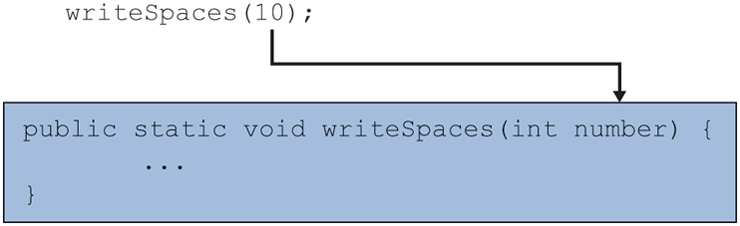
\includegraphics[width=\maxwidth,height=\maxheight,keepaspectratio,alt={Image}]{Figures/img_p6_0.png}}
\end{center}


\caption{Image}
\end{figure}

Tham số \texttt{number} là một biến cục bộ, nhưng nó nhận giá trị ban
đầu từ lời gọi. Gọi phương thức này với giá trị \texttt{10} tương đương
với việc bao gồm khai báo sau ở phần đầu của phương thức
\texttt{writeSpaces}:

\begin{verbatim}
int number = 10;
\end{verbatim}

Tất nhiên, cơ chế này linh hoạt hơn so với một khai báo biến cụ thể, bởi
vì thay vào đó, bạn có thể viết:

\begin{verbatim}
writeSpaces(20);
\end{verbatim}

và nó sẽ giống như thể bạn đã viết:

\begin{verbatim}
int number = 20;
\end{verbatim}

ở phần đầu của phương thức. Thậm chí bạn có thể sử dụng một biểu thức số
nguyên cho lời gọi:

\begin{verbatim}
writeSpaces(3 * 4 - 5);
\end{verbatim}

Trong trường hợp này, Java tính toán biểu thức để nhận được giá trị
\texttt{7} và sau đó gọi \texttt{writeSpaces}, khởi tạo \texttt{number}
bằng \texttt{7}.

Các nhà khoa học máy tính sử dụng từ ``tham số'' (parameter) theo nghĩa
rộng để chỉ cả những gì xuất hiện trong phần tiêu đề phương thức (tham
số hình thức) và những gì xuất hiện trong lời gọi phương thức (tham số
thực tế).

\textbf{Tham số Hình thức (Formal Parameter)} \textgreater{} Một biến
xuất hiện bên trong dấu ngoặc đơn ở phần tiêu đề của một phương thức,
được sử dụng để khái quát hóa (generalize) hành vi của phương thức đó.

\textbf{Tham số Thực tế (Actual Parameter)} \textgreater{} Một giá trị
hoặc một biểu thức cụ thể xuất hiện bên trong dấu ngoặc đơn trong một
lời gọi phương thức.

Thuật ngữ ``tham số hình thức'' không mô tả mục đích của nó. Một cái tên
tốt hơn sẽ là ``tham số khái quát'' (generalized parameter). Trong
phương thức \texttt{writeSpaces}, \texttt{number} là tham số khái quát
xuất hiện trong khai báo phương thức. Nó là một chỗ giữ (placeholder)
cho một số giá trị chưa được chỉ định. Các giá trị xuất hiện trong các
lời gọi phương thức là các tham số thực tế, bởi vì mỗi lời gọi chỉ ra
một tác vụ cụ thể cần thực hiện. Nói cách khác, mỗi lời gọi cung cấp một
giá trị thực tế để điền vào chỗ giữ.

Từ ``đối số'' (argument) thường được sử dụng như một từ đồng nghĩa với
``tham số'', chẳng hạn như trong câu ``Đây là những đối số (arguments)
tôi đang truyền cho phương thức này''. Một số người thích dành từ ``đối
số'' (argument) cho các tham số thực tế và từ ``tham số'' (parameter)
cho các tham số hình thức.

Hãy xem xét một ví dụ về cách bạn có thể sử dụng phương thức
\texttt{writeSpaces} này. Hãy nhớ rằng chương trình \texttt{DrawFigure2}
có phương thức sau đây, được gọi là \texttt{drawTop}:

\begin{verbatim}
// produces the top half of the hourglass figure
public static void drawTop() {
    for (int line = 1; line <= SUB_HEIGHT; line++) {
        System.out.print("|");
        for (int i = 1; i <= (line - 1); i++) {
            System.out.print(" ");
        }
        System.out.print("\\");
        int dots = 2 * SUB_HEIGHT - 2 * line;
        for (int i = 1; i <= dots; i++) {
            System.out.print(".");
        }
        System.out.print("/");
        for (int i = 1; i <= (line - 1); i++) {
            System.out.print(" ");
        }
        System.out.println("|");
    }
}
\end{verbatim}

Bằng cách sử dụng phương thức \texttt{writeSpaces}, bạn có thể viết lại
phương thức này như sau:

\begin{verbatim}
public static void drawTop() {
    for (int line = 1; line <= SUB_HEIGHT; line++) {
        System.out.print("|");
        writeSpaces(line - 1);
\end{verbatim}

\begin{verbatim}
    System.out.println("|");
}
\end{verbatim}

\}

\begin{verbatim}

Lưu ý rằng `writeSpaces` được gọi ở hai thời điểm khác nhau, chỉ định số lượng khoảng trắng cần thiết trong mỗi trường hợp. Bạn có thể sửa đổi phương thức `drawBottom` từ chương trình `DrawFigure2` theo cách tương tự để đơn giản hóa nó.

Bạn có thể viết toàn bộ một phương thức trong JShell để kiểm tra các tham số. Dưới đây là một phương thức có tên `writeStars` để in một số lượng dấu hoa thị nhất định ra giao diện điều khiển (console):
```java
jshell> public static void writeStars(int number) {
   ...>     for (int i = 1; i <= number; i++) {
   ...>         System.out.print("*");
   ...>     }
   ...> }
|  created method writeStars(int)
\end{verbatim}

\begin{verbatim}
jshell> writeStars(5);
*****
jshell> writeStars(8);
********
\end{verbatim}

\subsubsection{Cơ chế của các Tham số (The Mechanics of
Parameters)}\label{cux1a1-chux1ebf-cux1ee7a-cuxe1c-tham-sux1ed1-the-mechanics-of-parameters}

Khi Java thực thi một lời gọi đến một phương thức, nó sẽ khởi tạo các
tham số của phương thức đó. Đối với mỗi tham số, đầu tiên nó sẽ tính
toán biểu thức được truyền vào dưới dạng tham số thực tế (actual
parameter) và sau đó sử dụng kết quả đó để khởi tạo biến cục bộ có tên
được cung cấp bởi tham số hình thức (formal parameter).

Hãy sử dụng một ví dụ để làm rõ quá trình này:

\begin{verbatim}
 1  // Demonstrates parameters with a method for writing spaces.
 2  public class ParameterExample {
 3      public static void main(String[] args) {
\end{verbatim}

\begin{verbatim}
 4          int spaces1 = 3;
 5          int spaces2 = 5;
 6
 7          System.out.print("*");
 8          writeSpaces(spaces1);
 9          System.out.println("*");
 10
 11          System.out.print("!");
 12          writeSpaces(spaces2);
 13          System.out.println("!");
 14
 15          System.out.print("'");
 16          writeSpaces(8);
 17          System.out.println("'");
 18
 19          System.out.print("<");
 20          writeSpaces(spaces1 * spaces2 - 5);
 21          System.out.println(">");
 22      }
 23
 24      // writes "number" spaces on the current output line
 25      public static void writeSpaces(int number) {
 26          for (int i = 1; i <= number; i++) {
 27              System.out.print(" ");
 28          }
 29      }
 30  }
\end{verbatim}

Trong hai dòng đầu tiên của phương thức \texttt{main}, máy tính tìm thấy
các lệnh để cấp phát và khởi tạo hai biến:

Ba dòng mã tiếp theo tạo ra một dòng kết quả đầu ra với ba khoảng trắng
được bao quanh bởi các dấu hoa thị ở hai bên:

\begin{verbatim}
System.out.print("*");
writeSpaces(spaces1);
System.out.println("*");
\end{verbatim}

Bạn có thể thấy các dấu hoa thị đến từ đâu, nhưng hãy nhìn vào lời gọi
phương thức tạo ra các khoảng trắng. Khi Java thực thi lời gọi tới
\texttt{writeSpaces}, nó phải thiết lập tham số của nó. Để thiết lập
tham số, đầu tiên Java tính toán biểu thức được truyền vào dưới dạng
tham số thực tế. Biểu thức này đơn giản là biến \texttt{spaces1}, biến
có giá trị là \texttt{3}. Do đó, biểu thức được tính toán ra \texttt{3}.
Java sử dụng kết quả này để khởi tạo một biến cục bộ có tên là
\texttt{number}.

Sơ đồ dưới đây chỉ ra cách bộ nhớ của máy tính sẽ trông như thế nào khi
phương thức \texttt{writeSpaces} được tiến vào lần đầu tiên. Bởi vì có
hai phương thức liên quan (là \texttt{main} và \texttt{writeSpaces}), sơ
đồ sẽ chỉ ra những biến nào là cục bộ đối với \texttt{main}
(\texttt{spaces1} và \texttt{spaces2}) và những biến nào là cục bộ đối
với \texttt{writeSpaces} (tham số \texttt{number}):

\begin{figure}
\centering


\begin{center}
\pandocbounded{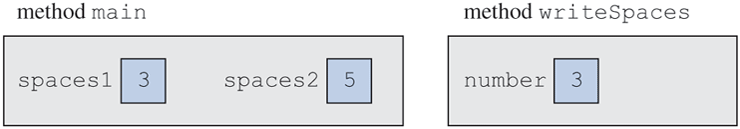
\includegraphics[width=\maxwidth,height=\maxheight,keepaspectratio,alt={Image}]{Figures/img_p14_0.png}}
\end{center}


\caption{Image}
\end{figure}

Tác dụng thực tế của quá trình này là phương thức \texttt{writeSpaces}
có một bản sao cục bộ của giá trị được lưu trong biến \texttt{spaces1}
từ phương thức \texttt{main}. Câu lệnh \texttt{println} xuất hiện sau
lời gọi tới \texttt{writeSpaces} sẽ đặt một dấu hoa thị vào cuối dòng và
sau đó hoàn thành dòng kết quả đầu ra.

Bây giờ hãy theo dõi ba dòng mã tiếp theo:

\begin{verbatim}
System.out.print("!");
writeSpaces(spaces2);
System.out.println("!");
\end{verbatim}

Dòng đầu tiên in ra một dấu chấm than trên dòng kết quả đầu ra thứ hai,
sau đó gọi \texttt{writeSpaces} một lần nữa, lần này với biến
\texttt{spaces2} là tham số thực tế của nó. Máy tính tính toán biểu thức
này, thu được kết quả \texttt{5}. Giá trị này được sử dụng để khởi tạo
\texttt{number}. Như vậy,

lần này nó tạo ra một bản sao của giá trị được lưu trong biến
\texttt{spaces2} từ phương thức \texttt{main}:

\begin{figure}
\centering


\begin{center}
\pandocbounded{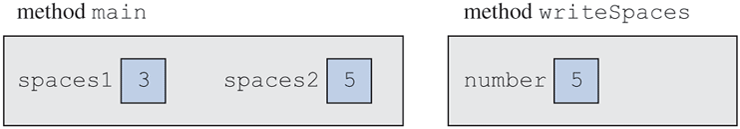
\includegraphics[width=\maxwidth,height=\maxheight,keepaspectratio,alt={Image}]{Figures/img_p15_0.png}}
\end{center}


\caption{Image}
\end{figure}

Vì lần này \texttt{number} có một giá trị khác (\texttt{5} thay vì
\texttt{3}), phương thức tạo ra một số lượng khoảng trắng khác. Sau khi
phương thức thực thi, \texttt{println} kết thúc dòng kết quả đầu ra bằng
một dấu chấm than thứ hai.

Dưới đây là ba dòng mã tiếp theo:

\begin{verbatim}
System.out.print("'");
writeSpaces(8);
System.out.println("'");
\end{verbatim}

Đoạn mã này in ra một dấu nháy đơn ở đầu dòng kết quả đầu ra thứ ba và
sau đó gọi lại \texttt{writeSpaces}. Lần này nó sử dụng hằng số nguyên
\texttt{8} làm biểu thức, điều đó có nghĩa là nó khởi tạo tham số
\texttt{number} như một bản sao của số \texttt{8}:

\begin{figure}
\centering


\begin{center}
\pandocbounded{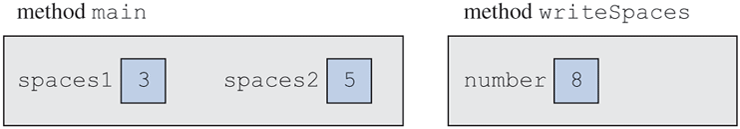
\includegraphics[width=\maxwidth,height=\maxheight,keepaspectratio,alt={Image}]{Figures/img_p16_0.png}}
\end{center}


\caption{Image}
\end{figure}

Một lần nữa, phương thức sẽ hoạt động khác đi do giá trị khác nhau của
\texttt{number}. Nó in ra tám khoảng trắng trên dòng và kết thúc thực
thi. Sau đó \texttt{println} hoàn thành dòng kết quả đầu ra bằng cách in
một dấu nháy đơn khác ở cuối dòng.

Cuối cùng, ba dòng mã cuối cùng trong phương thức \texttt{main} là:

\begin{verbatim}
System.out.print("<");
writeSpaces(spaces1 * spaces2 - 5);
System.out.println(">");
\end{verbatim}

Đoạn mã này in ra một ký tự nhỏ hơn (\texttt{\textless{}}) ở đầu dòng
kết quả đầu ra thứ tư và sau đó thực hiện lời gọi cuối cùng tới phương
thức \texttt{writeSpaces}. Lần này tham số thực tế là một biểu thức,
không chỉ là một biến hay một giá trị hằng. Do đó, trước khi lời gọi
được thực hiện, máy tính sẽ tính toán biểu thức để xác định giá trị của
nó:

\begin{figure}
\centering


\begin{center}
\pandocbounded{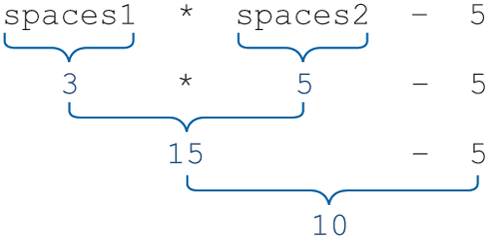
\includegraphics[width=\maxwidth,height=\maxheight,keepaspectratio,alt={Image}]{Figures/img_p17_0.png}}
\end{center}


\caption{Image}
\end{figure}

Máy tính sử dụng kết quả này để khởi tạo \texttt{number}:

\begin{figure}
\centering


\begin{center}
\pandocbounded{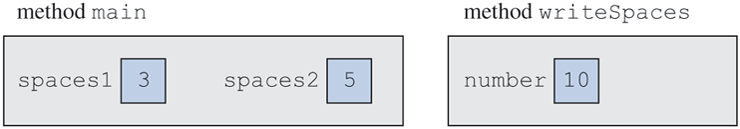
\includegraphics[width=\maxwidth,height=\maxheight,keepaspectratio,alt={Image}]{Figures/img_p17_1.png}}
\end{center}


\caption{Image}
\end{figure}

Bây giờ \texttt{number} là một bản sao của giá trị được mô tả bởi biểu
thức phức tạp này. Vì vậy, tổng kết quả đầu ra của chương trình này là:

\begin{verbatim}
*   * 
!     ! 
'       ' 
<         >
\end{verbatim}

\begin{quote}
\textbf{LỖI LẬP TRÌNH PHỔ BIẾN (COMMON PROGRAMMING ERROR)}

\textbf{Nhầm lẫn giữa các Tham số Thực tế và Hình thức (Confusing Actual
and Formal Parameters)}

Nhiều sinh viên đã quen với việc nhìn thấy các khai báo của các tham số
hình thức và lầm tưởng rằng cú pháp của chúng giống hệt với cú pháp
truyền các tham số thực tế. Một sai lầm phổ biến là viết cả kiểu của một
biến khi nó đang được truyền vào như một tham số:

\begin{verbatim}
writeSpaces(int spaces1); // this doesn’t work
\end{verbatim}

Sự nhầm lẫn này là do kiểu của tham số được viết trong phần khai báo của
phương thức, giống như thế này:

\begin{verbatim}
public static void writeSpaces(int number)
\end{verbatim}

Các kiểu (types) phải được viết ra khi các biến hoặc các tham số được
khai báo, nhưng khi các biến được sử dụng, chẳng hạn như khi mã gọi một
phương thức và truyền các biến vào dưới dạng các tham số thực tế, thì
kiểu của chúng sẽ không được viết. Các tham số thực tế không phải là các
khai báo; do đó, các kiểu không nên được viết trước chúng:

\begin{verbatim}
writeSpaces(spaces1); // much better!
\end{verbatim}
\end{quote}

\subsubsection{Những hạn chế của Tham số (Limitations of
Parameters)}\label{nhux1eefng-hux1ea1n-chux1ebf-cux1ee7a-tham-sux1ed1-limitations-of-parameters}

Chúng ta đã thấy rằng một tham số có thể được sử dụng để cung cấp đầu
vào cho một phương thức. Nhưng trong khi bạn có thể sử dụng một tham số
để gửi một giá trị vào một phương thức, bạn không thể sử dụng một tham
số để lấy một giá trị ra khỏi một phương thức. Khi một tham số được
thiết lập, một biến cục bộ được tạo ra và được khởi tạo bằng giá trị
được truyền vào dưới dạng tham số thực tế. Tác dụng thực tế là biến cục
bộ đó là một bản sao của giá trị đến từ bên ngoài. Vì nó là một biến cục
bộ, nó không thể ảnh hưởng đến bất kỳ biến nào bên ngoài phương thức.
Hãy xem xét chương trình mẫu sau:

\begin{verbatim}
 1  // A demonstration of parameter limitations.
 2  public class ParameterExample2 {
 3      public static void main(String[] args) {
 4          int x = 17;
 5          doubleNumber(x);
 6          System.out.println("x = " + x);
 7          System.out.println();
 8
 9          int number = 42;
\end{verbatim}

10 doubleNumber(number); 11 System.out.println(``number ='' + number);
12 \} 13 14 public static void doubleNumber(int number) \{ 15
System.out.println(``Initial value ='' + number); 16 number = number *
2; 17 System.out.println(``Final value ='' + number); 18 \} 19 \}

\begin{verbatim}

Chương trình này bắt đầu bằng việc khai báo và khởi tạo một biến số nguyên được gọi là `x` với giá trị `17`:



Sau đó, nó gọi phương thức `doubleNumber`, truyền `x` vào dưới dạng một tham số. Giá trị của `x` được sử dụng để khởi tạo tham số `number` như một biến cục bộ của phương thức có tên `doubleNumber`:

![Image](Figures/img_p21_0.png)

Tiếp theo, chương trình thực thi các câu lệnh bên trong `doubleNumber`. Đầu tiên, `doubleNumber` in ra giá trị ban đầu của `number` (`17`). Sau đó, nó nhân đôi `number`:

![Image](Figures/img_p21_1.png)

Lưu ý rằng điều này không có tác động gì đến biến `x`. Tham số được gọi là `number` là một bản sao của `x`, vì vậy mặc dù chúng bắt đầu giống nhau, việc thay đổi giá trị của `number` không làm ảnh hưởng đến `x`. Tiếp đó, `doubleNumber` báo cáo giá trị mới của `number` (`34`).

Tại thời điểm này, `doubleNumber` kết thúc thực thi và chúng ta trở về `main`:



Câu lệnh tiếp theo trong phương thức `main` báo cáo giá trị của `x`, đó là `17`. Sau đó, nó khai báo và khởi tạo một biến được gọi là `number` với giá trị `42`:



Câu lệnh sau đó gọi `doubleNumber` một lần nữa, lần này truyền cho nó giá trị của `number`. Đây là một tình huống kỳ lạ vì tham số này có cùng tên với biến trong `main`, nhưng Java không quan tâm. Nó luôn tạo ra một biến cục bộ mới cho phương thức `doubleNumber`:



Vì vậy, tại thời điểm này có hai biến khác nhau được gọi là `number`, mỗi biến ở một phương thức. Bây giờ là lúc để thực thi các câu lệnh của `doubleNumber` một lần nữa. Đầu tiên nó báo cáo giá trị của `number` (`42`), sau đó nhân đôi nó:



Một lần nữa, lưu ý rằng việc nhân đôi `number` bên trong `doubleNumber` không có tác động gì đến biến ban đầu `number` trong `main`. Đây là các biến riêng biệt. Phương thức sau đó báo cáo giá trị mới của `number` (`84`) và trở về `main`:



Tiếp đó, chương trình báo cáo giá trị của `number` và kết thúc. Vì vậy, tổng thể kết quả đầu ra của chương trình như sau:
```text
Initial value = 17 
Final value = 34 
x = 17 
 
Initial value = 42 
Final value = 84 
number = 42
\end{verbatim}

Các thao tác cục bộ đối với tham số không làm thay đổi những biến này ở
bên ngoài phương thức. Việc các biến được sao chép là một khía cạnh quan
trọng của các tham số. Về mặt tích cực, chúng ta biết rằng các biến được
bảo vệ khỏi sự thay đổi vì các tham số là những bản sao của biến gốc. Về
mặt tiêu cực, điều này có nghĩa là mặc dù các tham số sẽ cho phép chúng
ta gửi các giá trị vào một phương thức, chúng sẽ không cho phép chúng ta
lấy các giá trị trở lại ra khỏi một phương thức.

\subsubsection{Nhiều Tham số (Multiple
Parameters)}\label{nhiux1ec1u-tham-sux1ed1-multiple-parameters}

Cho đến nay, cuộc thảo luận của chúng ta về cú pháp của tham số vẫn mang
tính không chính thức. Đã đến lúc chúng ta viết ra một cách chính xác
hơn cú pháp chúng ta sử dụng để khai báo các phương thức tĩnh có chứa
tham số. Dưới đây là cú pháp đó:

\begin{verbatim}
public static void <name>(<type> <name>, ..., <type> <name>) {
    <statement>;
    <statement>;
    ...
\end{verbatim}

\begin{verbatim}
    <statement>;
}
\end{verbatim}

Bản mẫu (template) này chỉ ra rằng chúng ta có thể khai báo bao nhiêu
tham số tùy thích bên trong cặp ngoặc đơn xuất hiện sau tên của một
phương thức trong tiêu đề của nó. Chúng ta sử dụng dấu phẩy để phân tách
các tham số khác nhau.

Lấy ví dụ về một phương thức có nhiều tham số, hãy xem xét một biến thể
của \texttt{writeSpaces}. Thật tiện lợi khi chúng ta có thể sử dụng
phương thức này để in ra số lượng khoảng trắng khác nhau, nhưng nó luôn
chỉ in khoảng trắng. Điều gì sẽ xảy ra nếu chúng ta muốn 18 dấu hoa thị,
hoặc 23 dấu chấm, hay 17 dấu chấm hỏi? Chúng ta có thể khái quát hóa tác
vụ này xa hơn nữa bằng cách cho phương thức nhận hai tham số---một ký tự
và số lần in ký tự đó:

\begin{verbatim}
public static void writeChars(char ch, int number) {
    for (int i = 1; i <= number; i++) {
        System.out.print(ch);
    }
}
\end{verbatim}

Ký tự cần in ra là một tham số có kiểu \texttt{char}, chúng ta sẽ thảo
luận chi tiết hơn về kiểu này trong chương tiếp theo. Hãy nhớ lại rằng
các hằng ký tự (character literals) được đặt trong các dấu nháy đơn.

Bản mẫu cú pháp để gọi một phương thức nhận tham số là như sau:

\begin{verbatim}
<method name>(<expression>, <expression>, ..., <expression>);
\end{verbatim}

Bằng cách gọi phương thức \texttt{writeChars}, bạn có thể viết mã giống
như sau:

\begin{verbatim}
writeChars('=', 20);
System.out.println();
for (int i = 1; i <= 10; i++) {
    writeChars('>', i);
    writeChars(' ', 20 - 2 * i);
    writeChars('<', i);
    System.out.println();
}
\end{verbatim}

Đoạn mã này tạo ra kết quả đầu ra sau:

\begin{verbatim}
==================== 
>                  < 
>>                << 
>>>              <<< 
>>>>            <<<< 
>>>>>          <<<<< 
>>>>>>        <<<<<< 
>>>>>>>      <<<<<<< 
>>>>>>>>    <<<<<<<< 
>>>>>>>>>  <<<<<<<<< 
>>>>>>>>>><<<<<<<<<<
\end{verbatim}

Bằng cách sử dụng phương thức \texttt{writeChars}, chúng ta có thể viết
một phiên bản thậm chí còn tốt hơn của phương thức \texttt{drawTop} từ
chương trình \texttt{DrawFigure2} ở Chương 2.

Chúng ta đã thấy trước đó rằng bằng cách sử dụng \texttt{writeSpaces},
chúng ta có thể loại bỏ hai trong số các vòng lặp bên trong, nhưng điều
này vẫn để lại cho chúng ta vòng lặp bên trong để in các dấu chấm. Bây
giờ, chúng ta có thể loại bỏ tất cả ba vòng lặp bên trong và tạo ra một
phiên bản dễ đọc hơn nhiều của phương thức này:

\begin{verbatim}
public static void drawTop() {
    for (int line = 1; line <= SUB_HEIGHT; line++) {
        System.out.print("|");
        writeChars(' ', line - 1);
        System.out.print("\\");
        writeChars('.', 2 * SUB_HEIGHT - 2 * line);
        System.out.print("/");
        writeChars(' ', line - 1);
        System.out.println("|");
    }
}
\end{verbatim}

Bạn có thể bao gồm bao nhiêu tham số tùy thích khi bạn định nghĩa một
phương thức. Mỗi lời gọi phương thức phải cung cấp chính xác số lượng
tham số đó, theo cùng một thứ tự. Ví dụ, hãy xem xét lời gọi đầu tiên
tới \texttt{writeChars} trong đoạn mã trước đó và tiêu đề của
\texttt{writeChars}. Java xếp hàng các tham số theo thứ tự tuần tự (với
tham số thực tế đầu tiên đi vào tham số hình thức đầu tiên và tham số
thực tế thứ hai đi vào tham số hình thức thứ hai):

\begin{figure}
\centering


\begin{center}
\pandocbounded{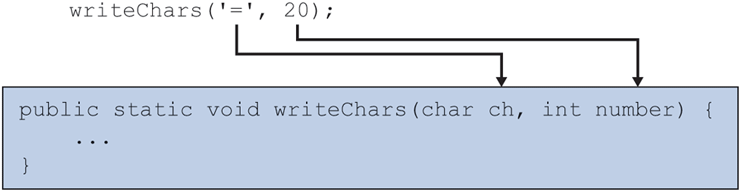
\includegraphics[width=\maxwidth,height=\maxheight,keepaspectratio,alt={Image}]{Figures/img_p28_0.png}}
\end{center}


\caption{Image}
\end{figure}

Chúng ta đã thấy rằng các phương thức có thể gọi các phương thức khác;
điều này cũng đúng với các phương thức nhận tham số. Ví dụ, đây là một
phương thức dùng để vẽ một hộp có chiều cao và chiều rộng nhất định có
gọi đến phương thức \texttt{writeChars}:

\begin{verbatim}
public static void drawBox(int height, int width) {
    // draw top of box
    writeChars('*', width);
    System.out.println();

    // draw middle lines
    for (int i = 1; i <= height - 2; i++) {
        System.out.print('*');
        writeChars(' ', width - 2);
        System.out.println("*");
    }
    // draw bottom of box
    writeChars('*', width);
    System.out.println();
}
\end{verbatim}

Lưu ý rằng \texttt{drawBox} được truyền các giá trị cho các tham số có
tên là \texttt{height} và \texttt{width}, và các tham số này được sử
dụng để tạo thành các biểu thức được truyền dưới dạng giá trị cho
\texttt{writeChars}. Ví dụ, bên trong vòng lặp \texttt{for}, chúng ta
gọi \texttt{writeChars} yêu cầu nó tạo ra \texttt{width\ -\ 2} khoảng
trắng. (Chúng ta trừ đi 2 vì chúng ta in một dấu sao ở đầu và ở cuối
dòng.) Dưới đây là một lời gọi mẫu tới phương thức này:

\begin{verbatim}
drawBox(5, 10);
\end{verbatim}

Đoạn mã này tạo ra kết quả đầu ra sau:

\begin{center}\rule{0.5\linewidth}{0.5pt}\end{center}

\begin{itemize}
\item
\begin{verbatim}
   * 
\end{verbatim}
\item
\begin{verbatim}
   * 
\end{verbatim}
\item
\begin{verbatim}
   * 
\end{verbatim}

  \begin{center}\rule{0.5\linewidth}{0.5pt}\end{center}
\end{itemize}

\begin{verbatim}

Khi bạn viết các phương thức nhận nhiều tham số, phần tiêu đề phương thức có thể trở nên rất dài. Người ta thường ngắt các dòng dài (những dòng vượt quá khoảng 80 ký tự) bằng cách chèn một ngắt dòng sau một toán tử hoặc một tham số và thụt lề dòng tiếp theo bằng hai lần độ rộng thụt lề thông thường:
```java
// this method’s header is too long, so we’ll wrap it
public static void printTriangle(int xCoord1, int yCoord1,
        int xCoord2, int yCoord2, int xCoord3, int yCoord3) {
  ...
}
\end{verbatim}

\subsubsection{Tham số so với Hằng số (Parameters versus
Constants)}\label{tham-sux1ed1-so-vux1edbi-hux1eb1ng-sux1ed1-parameters-versus-constants}

Trong Chương 2, bạn đã thấy rằng các hằng số của lớp là một cơ chế hữu
ích để tăng tính linh hoạt cho các chương trình của bạn. Bằng cách sử
dụng các hằng số như vậy, bạn có thể dễ dàng sửa đổi một chương trình để
nó hoạt động khác đi. Các tham số cung cấp nhiều sự linh hoạt tương tự,
và còn nhiều hơn thế. Hãy xem xét phương thức \texttt{writeSpaces}. Giả
sử bạn viết nó bằng cách sử dụng một hằng số của lớp:

\begin{verbatim}
public static final int NUMBER_OF_SPACES = 10;
\end{verbatim}

Cách tiếp cận này sẽ mang lại cho bạn sự linh hoạt để tạo ra một số
lượng khoảng trắng khác nhau, nhưng nó có một hạn chế lớn: Hằng số chỉ
có thể thay đổi từ lần thực thi này sang lần thực thi khác; nó không thể
thay đổi trong một lần thực thi duy nhất. Nói cách khác, bạn có thể thực
thi chương trình một lần với một giá trị, chỉnh sửa chương trình, biên
dịch lại, và sau đó thực thi lại với một giá trị khác, nhưng bạn không
thể sử dụng các giá trị khác nhau trong một lần thực thi chương trình
nếu sử dụng một hằng số của lớp.

Các tham số thì linh hoạt hơn. Bởi vì bạn chỉ định giá trị sẽ được sử
dụng mỗi khi bạn gọi phương thức, bạn có thể sử dụng một vài giá trị
khác nhau trong một lần thực thi chương trình. Như bạn đã thấy, bạn có
thể gọi phương thức nhiều lần khác nhau trong một lần thực thi chương
trình và làm cho nó hoạt động khác nhau ở mỗi lần. Tuy nhiên, việc sử
dụng các tham số đòi hỏi lập trình viên phải làm nhiều việc hơn so với
việc sử dụng các hằng số của lớp. Nó làm cho các tiêu đề phương thức và
các lời gọi phương thức trở nên tẻ nhạt hơn, chưa kể đến việc làm cho
quá trình thực thi (và do đó, quá trình gỡ lỗi) trở nên phức tạp hơn.

Vì vậy, có thể bạn sẽ tìm thấy dịp để sử dụng mỗi kỹ thuật. Quy tắc cơ
bản là hãy sử dụng một hằng số của lớp khi bạn chỉ muốn thay đổi giá trị
từ lần thực thi này sang lần thực thi khác. Nếu bạn muốn sử dụng các giá
trị khác nhau trong một lần thực thi duy nhất, hãy sử dụng một tham số.

\subsubsection{Nạp chồng Phương thức (Overloading of
Methods)}\label{nux1ea1p-chux1ed3ng-phux1b0ux1a1ng-thux1ee9c-overloading-of-methods}

Bạn sẽ thường muốn tạo ra những biến thể nhỏ của cùng một phương thức
bằng cách truyền vào các tham số khác nhau. Ví dụ, bạn có thể có một
phương thức \texttt{drawBox} cho phép bạn chỉ định một chiều cao và
chiều rộng cụ thể, nhưng bạn cũng có thể muốn có một phiên bản vẽ một
cái hộp với kích thước mặc định. Nói cách khác, đôi khi bạn muốn chỉ
định các giá trị này, như trong:

\begin{verbatim}
drawBox(8, 10);
\end{verbatim}

và những lần khác bạn chỉ muốn vẽ một cái hộp với chiều cao và chiều
rộng tiêu chuẩn:

\begin{verbatim}
drawBox();
\end{verbatim}

Một số ngôn ngữ lập trình yêu cầu bạn phải nghĩ ra các tên khác nhau cho
những phiên bản này, chẳng hạn như \texttt{drawBox} và
\texttt{drawDefaultBox}. Như bạn có thể tưởng tượng, việc nghĩ ra tên
mới cho mỗi biến thể trở nên tẻ nhạt. Thật may mắn, Java cho phép bạn có
nhiều hơn một phương thức có cùng tên, miễn là chúng có các tham số khác
nhau. Điều này được gọi là nạp chồng (overloading). Yêu cầu chính đối
với việc nạp chồng là các phương thức khác nhau mà bạn định nghĩa phải
có các chữ ký phương thức (method signatures) khác nhau.

\begin{quote}
\textbf{Nạp chồng Phương thức (Method Overloading)}

Khả năng định nghĩa hai hoặc nhiều phương thức khác nhau có cùng tên
nhưng khác chữ ký phương thức.

\textbf{Chữ ký Phương thức (Method Signature)}

Tên của một phương thức, cùng với số lượng và kiểu của các tham số của
nó.
\end{quote}

Hai phiên bản \texttt{drawBox} trong ví dụ rõ ràng có các chữ ký phương
thức khác nhau, bởi vì một phương thức có hai tham số và phương thức kia
có không tham số. Từ bất kỳ lời gọi nào tới phương thức cũng sẽ rõ ràng
về việc sử dụng phiên bản nào: Nếu bạn thấy có hai tham số, bạn thực thi
phiên bản có hai tham số; nếu bạn thấy không có tham số nào, bạn thực
thi phiên bản có không tham số.

Tình huống trở nên phức tạp hơn khi việc nạp chồng liên quan đến cùng
một số lượng tham số, nhưng điều này hóa ra lại là một trong những ứng
dụng hữu ích nhất của việc nạp chồng. Ví dụ, phương thức
\texttt{println} thực tế là một chuỗi các phương thức được nạp chồng.
Chúng ta có thể gọi \texttt{println} bằng cách truyền cho nó một
\texttt{String}, một \texttt{int}, một \texttt{double}, v.v. Sự linh
hoạt này được triển khai dưới dạng một loạt các phương thức khác nhau,
tất cả đều nhận một tham số: Một phiên bản nhận một \texttt{String}, một
phiên bản khác nhận một \texttt{int}, một phiên bản khác nữa nhận một
\texttt{double}, và cứ tiếp tục như vậy. Rõ ràng là bạn thực hiện các
thao tác hơi khác nhau để in ra một trong những loại dữ liệu này so với
các loại dữ liệu khác, đó là lý do tại sao việc có các phiên bản khác
nhau của phương thức là rất hữu ích.

\subsection{Các Phương thức Trả về Giá trị (Methods That Return
Values)}\label{cuxe1c-phux1b0ux1a1ng-thux1ee9c-trux1ea3-vux1ec1-giuxe1-trux1ecb-methods-that-return-values-1}

Vài phương thức cuối cùng mà chúng ta đã xem xét là các phương thức định
hướng hành động (action-oriented) nhằm thực hiện một số tác vụ cụ thể.
Bạn có thể coi chúng giống như các mệnh lệnh mà bạn có thể ra lệnh cho
ai đó, như ``Hãy vẽ một hộp'' hoặc ``Hãy vẽ một hình tam giác.'' Các
tham số cho phép các mệnh lệnh này trở nên linh hoạt hơn, như ``Hãy vẽ
một hộp có kích thước 10 x 20.''

Bạn cũng sẽ muốn có thể viết các phương thức dùng để tính toán các giá
trị. Những phương thức này giống như các câu hỏi hơn, như ``Căn bậc hai
của 2.5 là bao nhiêu?'' hoặc ``Bạn nhận được gì khi lũy thừa bậc 4 của
2.3?'' Lấy ví dụ, hãy xem xét một phương thức tên là \texttt{sqrt} sẽ
tính căn bậc hai của một số.

Có vẻ như cách để viết một phương thức như vậy sẽ là để nó nhận một tham
số kiểu \texttt{double} và in ra (bằng \texttt{println}) căn bậc hai của
nó ra giao diện điều khiển (console). Nhưng bạn có thể muốn sử dụng căn
bậc hai như một phần của một biểu thức hoặc một phép tính lớn hơn, chẳng
hạn như giải một phương trình bậc hai hoặc tính toán khoảng cách giữa
các điểm trên một mặt phẳng tọa độ \(x/y\).

Một giải pháp tốt hơn sẽ là một lệnh căn bậc hai (square root command)
truyền con số đang được quan tâm vào dưới dạng một tham số và trả về
(return) căn bậc hai của nó cho chương trình như một kết quả. Sau đó,
bạn có thể sử dụng kết quả đó như một phần của một biểu thức, lưu nó vào
một biến, hoặc in nó ra giao diện điều khiển. Một lệnh như vậy là một
kiểu phương thức mới được cho là sẽ trả về một giá trị.

\begin{quote}
\textbf{Trả về (Return)}

Việc gửi một giá trị ra ngoài dưới dạng kết quả của một phương thức có
thể được sử dụng trong một biểu thức trong chương trình của bạn. Các
phương thức void không trả về bất kỳ giá trị nào.
\end{quote}

Nếu bạn có một phương thức như vậy, bạn có thể yêu cầu lấy căn bậc hai
của 2.5 bằng cách viết đoạn mã như thế này:

\begin{verbatim}
// assuming you had a method called sqrt
double answer = sqrt(2.5);
\end{verbatim}

Phương thức \texttt{sqrt} có một tham số (số mà bạn muốn tìm căn bậc
hai), và nó cũng trả về một giá trị (căn bậc hai đó). Tham số thực tế
\texttt{2.5} đi ``vào trong'' phương thức, và căn bậc hai đi ra. Trong
đoạn mã trước, kết quả được trả về sẽ được lưu trong một biến có tên là
\texttt{answer}.

Bạn có thể biết được liệu một phương thức có trả về một giá trị hay
không bằng cách nhìn vào tiêu đề của nó. Tất cả các phương thức bạn đã
viết cho đến nay đều bắt đầu bằng \texttt{public\ static\ void}. Từ
\texttt{void} được gọi là kiểu trả về (return type) của phương thức.

Kiểu trả về \texttt{void} hơi kỳ lạ một chút bởi vì, đúng như tên gọi
của nó, phương thức không trả về gì cả. Một phương thức có thể trả về
bất kỳ kiểu hợp lệ nào: một \texttt{int}, một \texttt{double}, hoặc bất
kỳ kiểu nào khác. Trong trường hợp của phương thức \texttt{sqrt}, bạn
muốn nó trả về một \texttt{double}, vì vậy bạn sẽ viết tiêu đề của nó
như sau:

\begin{verbatim}
public static double sqrt(double n)
\end{verbatim}

Giống như trường hợp trước, từ đứng sau \texttt{public\ static} là kiểu
trả về của phương thức:

May mắn thay, bạn không thực sự cần phải viết một phương thức để tính
căn bậc hai của một số, bởi vì Java đã có sẵn một phương thức được tích
hợp (built in). Phương thức này được bao gồm trong một lớp có tên là
\texttt{Math}, lớp này bao gồm nhiều phương thức tính toán hữu ích. Vì
vậy, trước khi chúng ta thảo luận chi tiết về việc viết các phương thức
trả về các giá trị, hãy cùng khám phá lớp \texttt{Math} và xem nó cung
cấp những gì.

\subsubsection{Lớp Math (The Math
Class)}\label{lux1edbp-math-the-math-class}

Trong Chương 1, chúng ta đã đề cập rằng rất nhiều mã định nghĩa sẵn,
được gọi chung là các thư viện lớp Java (Java class libraries), đã được
viết cho Java. Một trong những lớp hữu ích nhất là \texttt{Math}. Nó bao
gồm các hằng số toán học được định nghĩa sẵn và một số lượng lớn các hàm
toán học thông dụng. Lớp \texttt{Math} sẽ có sẵn trên bất kỳ máy nào
được cài đặt Java đúng cách.

Như chúng ta đã lưu ý trong phần trước, lớp \texttt{Math} có một phương
thức tên là \texttt{sqrt} dùng để tính căn bậc hai của một số. Phương
thức này có tiêu đề như sau:

\begin{verbatim}
public static double sqrt(double n)
\end{verbatim}

Tiêu đề này nói rằng phương thức có tên là \texttt{sqrt}, nó nhận một
tham số kiểu \texttt{double}, và nó trả về một giá trị kiểu
\texttt{double}. Rất tiếc, bạn không thể chỉ gọi phương thức này trực
tiếp bằng cách dẫn chiếu đến nó là \texttt{sqrt} bởi vì nó nằm trong một
lớp khác. Bất cứ khi nào bạn muốn dẫn chiếu đến một cái gì đó được khai
báo trong một lớp khác, bạn sử dụng ký hiệu dấu chấm (dot notation):

\begin{verbatim}
<class name>.<element>
\end{verbatim}

Vì vậy, bạn sẽ dẫn chiếu tới phương thức này là \texttt{Math.sqrt}. Dưới
đây là một chương trình mẫu sử dụng phương thức này:

\begin{verbatim}
1  // Computes square roots using the Math class.
2  public class WriteRoots {
3      public static void main(String[] args) {
4          for (int i = 1; i <= 20; i++) {
5              double root = Math.sqrt(i);
6              System.out.println("sqrt(" + i + ") = " + root);
7          }
8      }
9  }
\end{verbatim}

Chương trình này tạo ra kết quả đầu ra sau:

\begin{verbatim}
sqrt(1) = 1.0 
sqrt(2) = 1.4142135623730951 
sqrt(3) = 1.7320508075688772 
sqrt(4) = 2.0 
sqrt(5) = 2.23606797749979 
sqrt(6) = 2.449489742783178 
sqrt(7) = 2.6457513110645907 
sqrt(8) = 2.8284271247461903 
sqrt(9) = 3.0 
sqrt(10) = 3.1622776601683795 
sqrt(11) = 3.3166247903554 
sqrt(12) = 3.4641016151377544 
\end{verbatim}

sqrt(13) = 3.605551275463989 sqrt(14) = 3.7416573867739413 sqrt(15) =
3.872983346207417 sqrt(16) = 4.0 sqrt(17) = 4.123105625617661 sqrt(18) =
4.242640687119285 sqrt(19) = 4.358898943540674 sqrt(20) =
4.47213595499958

\begin{verbatim}

Lưu ý rằng chúng ta đã truyền một giá trị có kiểu `int` cho `Math.sqrt`, nhưng tiêu đề cho biết rằng nó mong đợi một giá trị kiểu `double`. Hãy nhớ rằng nếu Java đang mong đợi một `double` và nhận được một `int`, nó sẽ chuyển đổi `int` đó thành một `double` tương ứng.

Lớp `Math` cũng định nghĩa hai hằng số thường được sử dụng: $e$ và $\pi$ (xem Bảng 3.1). Theo quy ước của Java, chúng ta sử dụng toàn bộ chữ in hoa cho tên của chúng và dẫn chiếu tới chúng là `Math.E` và `Math.PI`.

**Bảng 3.1 Các Hằng số Toán học (Math Constants)**



Bảng 3.2 liệt kê một số phương thức tĩnh hữu ích nhất từ lớp `Math`. Bạn có thể xem danh sách đầy đủ các phương thức được định nghĩa trong lớp `Math` bằng cách kiểm tra tài liệu API cho phiên bản Java của bạn. API mô tả cách sử dụng các thư viện chuẩn (standard libraries) có sẵn cho các lập trình viên Java. Nó có thể hơi choáng ngợp, vì các thư viện Java rất rộng lớn. Hãy dạo quanh một chút nếu bạn có hứng thú, nhưng đừng thất vọng vì có quá nhiều thư viện để lựa chọn trong Java.

**Bảng 3.2 Các Phương thức Tĩnh Hữu ích trong Lớp Math (Useful Static Methods in the Math Class)**

Tương tác JShell sau đây trình diễn một số phương thức `Math`:
```java
jshell> Math.ceil(2.13)
$1 ==> 3.0
jshell> Math.pow(2, 5)
$2 ==> 32.0
jshell> Math.random()
$3 ==> 0.6051518556439361
jshell> Math.sin(Math.PI / 2)
$4 ==> 1.0
jshell> Math.pow(2, 2) + Math.pow(3, 2)
$5 ==> 13.0
\end{verbatim}

Nếu bạn nhìn vào API của lớp \texttt{Math}, bạn sẽ nhận thấy rằng lớp
\texttt{Math} có một vài phương thức được nạp chồng (overloaded
methods). Ví dụ, có một phiên bản của phương thức giá trị tuyệt đối
(\texttt{Math.abs}) dành cho số nguyên và một phiên bản khác dành cho
kiểu \texttt{double}. Các quy tắc điều chỉnh việc phương thức nào được
gọi rất phức tạp, vì vậy chúng ta sẽ không đề cập đến chúng ở đây. Tuy
nhiên, ý tưởng cơ bản là Java cố gắng tìm ra phương thức phù hợp nhất.
Đối với hầu hết các trường hợp, bạn không cần phải suy nghĩ nhiều về vấn
đề này; bạn có thể để Java chọn thay bạn, và nó thường sẽ đưa ra lựa
chọn đúng đắn.

\subsubsection{Định nghĩa các Phương thức Trả về Giá trị (Defining
Methods That Return
Values)}\label{ux111ux1ecbnh-nghux129a-cuxe1c-phux1b0ux1a1ng-thux1ee9c-trux1ea3-vux1ec1-giuxe1-trux1ecb-defining-methods-that-return-values}

Bạn có thể viết các phương thức của riêng mình có trả về các giá trị
bằng cách sử dụng một câu lệnh đặc biệt được gọi là câu lệnh trả về
(return statement). Ví dụ, chúng ta thường sử dụng một phương thức trả
về một giá trị để biểu diễn một phương trình. Có một câu chuyện nổi
tiếng về nhà toán học Carl Friedrich Gauss minh họa việc sử dụng một
phương thức như vậy. Khi Gauss còn là một cậu bé, giáo viên của ông đã
yêu cầu cả lớp tính tổng các số nguyên từ 1 đến 100, với suy nghĩ rằng
họ sẽ mất một lúc để hoàn thành nhiệm vụ này. Gauss ngay lập tức tìm ra
một công thức và trình bày câu trả lời của mình cho giáo viên. Ông đã sử
dụng một thủ thuật đơn giản là cộng hai bản sao của chuỗi này với nhau,
một cái theo chiều xuôi và một cái theo chiều ngược. Phương pháp này cho
phép ông ghép cặp các giá trị từ hai bản sao để tổng của chúng giống
nhau:

Mỗi mục trong cột bên phải đều bằng 101 và có 100 hàng trong bảng này,
vì vậy tổng chung là \(100 \times 101 = 10100\). Tất nhiên, đó là tổng
của hai bản sao của chuỗi, vì vậy câu trả lời thực tế chỉ bằng một nửa
số đó. Sử dụng cách tiếp cận này, Gauss xác định rằng tổng của 100 số
nguyên đầu tiên là 5050. Khi chuỗi đi từ 1 đến \(n\), tổng là
\((n + 1) \times n/2\).

Chúng ta có thể sử dụng công thức của Gauss để viết một phương thức tính
tổng của \(n\) số nguyên đầu tiên:

\begin{verbatim}
// returns the sum of the integers 1-N, inclusive
public static int sum(int n) {
    return (n + 1) * n / 2;
}
\end{verbatim}

Phương thức \texttt{sum} có thể được sử dụng bởi phương thức
\texttt{main} trong đoạn mã như sau:

\begin{verbatim}
int answer = sum(100);
System.out.println("The sum of 1 through 100 is " + answer);
\end{verbatim}

Sơ đồ về những gì xảy ra khi đoạn mã này được thực thi như sau. Phương
thức được gọi (invoke) với tham số \texttt{n} được khởi tạo bằng 100.
Đưa giá trị này vào công thức, chúng ta nhận được giá trị 5050, giá trị
này được gửi trở lại để lưu vào biến có tên là \texttt{answer}:

\begin{figure}
\centering


\begin{center}
\pandocbounded{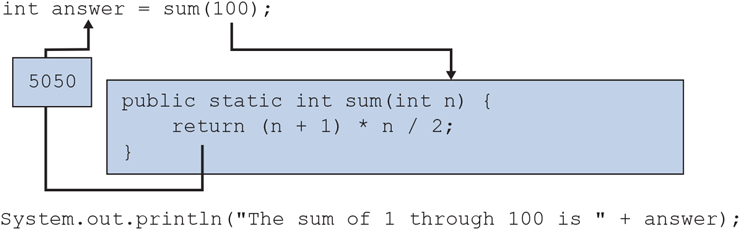
\includegraphics[width=\maxwidth,height=\maxheight,keepaspectratio,alt={Image}]{Figures/img_p44_0.png}}
\end{center}


\caption{Image}
\end{figure}

Một lần nữa, lưu ý rằng trong phần tiêu đề của phương thức, từ quen
thuộc \texttt{void} (chỉ ra rằng không có giá trị trả về) đã được thay
thế bằng từ \texttt{int}. Hãy nhớ rằng khi bạn khai báo một phương thức
trả về một giá trị, bạn phải báo cho Java biết loại giá trị nào nó sẽ
trả về. Do đó, chúng ta có thể cập nhật bản mẫu cú pháp của chúng ta cho
các phương thức tĩnh một lần nữa để làm rõ rằng phần tiêu đề bao gồm một
kiểu trả về (\texttt{void} cho không trả về):

\begin{verbatim}
public static <type> <name>(<type> <name>, ..., <type> <name>) 
{
    <statement>;
    <statement>;
    ...
    <statement>;
}
\end{verbatim}

Cú pháp của câu lệnh \texttt{return} là:

\begin{verbatim}
return <expression>;
\end{verbatim}

Khi Java gặp một câu lệnh \texttt{return}, nó tính toán biểu thức đã cho
và ngay lập tức kết thúc phương thức, trả về giá trị mà nó nhận được từ
biểu thức đó. Do đó, việc có bất kỳ câu lệnh nào khác sau một câu lệnh
\texttt{return} là không hợp lệ; \texttt{return} phải là câu lệnh cuối
cùng trong phương thức của bạn. Việc một phương thức Java có kiểu trả về
khác \texttt{void} kết thúc mà không có một lệnh \texttt{return} cũng là
một lỗi.

Có những ngoại lệ đối với các quy tắc trước đó, như bạn sẽ thấy sau này.
Ví dụ, việc một phương thức có nhiều hơn một câu lệnh \texttt{return} là
có thể xảy ra; điều này sẽ được đề cập trong chương tiếp theo, khi chúng
ta thảo luận về việc thực thi có điều kiện bằng các câu lệnh \texttt{if}
và \texttt{if/else}.

Hãy xem một phương thức mẫu khác có trả về một giá trị. Trong \emph{The
Wizard of Oz}, Bù Nhìn (Scarecrow) sau khi được cấp bằng tốt nghiệp đã
thể hiện sự thông minh của mình bằng cách mô tả một công thức sử dụng
tổng các căn bậc hai của hai cạnh bất kỳ của một tam giác cân. Có lẽ anh
ta đang cố gắng phát biểu định lý Pythagoras, mặc dù không rõ liệu những
người viết kịch bản dở toán hay họ đang đưa ra bình luận về giá trị của
một tấm bằng tốt nghiệp. Trong một tập phim của \emph{The Simpsons},
Homer lặp lại công thức sai lầm của Bù Nhìn sau khi đeo một cặp kính của
Henry Kissinger mà anh tìm thấy trong nhà vệ sinh tại nhà máy điện hạt
nhân Springfield.

Định lý Pythagoras chính xác chỉ áp dụng cho các tam giác vuông và phát
biểu rằng độ dài của cạnh huyền của một tam giác vuông bằng căn bậc hai
của tổng bình phương hai cạnh còn lại. Nếu bạn biết độ dài của hai cạnh
\(a\) và \(b\) của một tam giác vuông và muốn tìm độ dài của cạnh thứ ba
\(c\), bạn tính nó như sau: \(c = \sqrt{a^2 + b^2}\)

\begin{quote}
\textbf{LỖI LẬP TRÌNH PHỔ BIẾN (COMMON PROGRAMMING ERROR)}

\textbf{Bỏ qua Giá trị được Trả về (Ignoring the Returned Value)}

Khi bạn gọi một phương thức trả về một giá trị, kỳ vọng là bạn sẽ làm gì
đó với giá trị được trả về đó. Bạn có thể in nó ra, lưu nó vào một biến,
hoặc sử dụng nó như một phần của một biểu thức lớn hơn. Việc gọi phương
thức và chỉ đơn giản bỏ qua giá trị được trả về từ nó là hợp lệ (nhưng
không khôn ngoan):

\begin{verbatim}
sum(1000);   // doesn’t do anything
\end{verbatim}

Lời gọi ở trên không in ra tổng số cũng như không có bất kỳ tác dụng
đáng chú ý nào. Nếu bạn muốn giá trị được in ra, bạn phải bao gồm một
câu lệnh \texttt{println}:

\begin{verbatim}
int answer = sum(1000);    // better
System.out.println("Sum up to 1000 is " + answer);
\end{verbatim}

Một dạng ngắn hơn của đoạn mã đã sửa sẽ như sau:

\begin{verbatim}
System.out.println("Sum up to 1000 is " + sum(1000));
\end{verbatim}
\end{quote}

Giả sử bạn muốn in ra độ dài của các cạnh huyền của hai tam giác vuông,
một tam giác có độ dài các cạnh là 5 và 12, và tam giác còn lại có độ
dài các cạnh là 3 và 4. Bạn có thể viết đoạn mã như sau:

\begin{verbatim}
double c1 = Math.sqrt(Math.pow(5, 2) + Math.pow(12, 2));
System.out.println("hypotenuse 1 = " + c1);
double c2 = Math.sqrt(Math.pow(3, 2) + Math.pow(4, 2));
System.out.println("hypotenuse 2 = " + c2);
\end{verbatim}

Đoạn mã trước đó là chính xác, nhưng hơi khó đọc, và bạn sẽ phải lặp lại
cùng một phép toán phức tạp đó lần thứ ba nếu bạn muốn bao gồm một tam
giác thứ ba. Một giải pháp tốt hơn sẽ là tạo ra một phương thức để tính
toán và trả về độ dài cạnh huyền khi được truyền độ dài của hai cạnh kia
dưới dạng các tham số. Một phương thức như vậy sẽ trông giống như thế
này:

\begin{verbatim}
public static double hypotenuse(double a, double b) { 
    double c = Math.sqrt(Math.pow(a, 2) + Math.pow(b, 2)); 
    return c; 
}
\end{verbatim}

Phương thức này có thể được sử dụng để tạo ra một phương thức
\texttt{main} ngắn gọn và dễ đọc hơn, như được hiển thị dưới đây.

\begin{verbatim}
1  // Computes triangle hypotenuse lengths using return values. 
2  public class Triangles { 
3      public static void main(String[] args) { 
4          System.out.println("hypotenuse 1 = " + hypotenuse(5, 12)); 
5          System.out.println("hypotenuse 2 = " + hypotenuse(3, 4)); 
6      } 
7 
8      public static double hypotenuse(double a, double b) { 
9          double c = Math.sqrt(Math.pow(a, 2) + Math.pow(b, 2)); 
10         return c; 
11     } 
12 }
\end{verbatim}

Một số biến thể của chương trình này là có thể thực hiện. Thứ nhất,
không cần thiết phải lưu giá trị trả về của phương thức
\texttt{hypotenuse} vào biến \texttt{c}. Nếu muốn, bạn chỉ cần tính toán
và trả về giá trị đó trong một dòng duy nhất. Trong trường hợp này, phần
thân của phương thức \texttt{hypotenuse} sẽ trở thành như sau:

\begin{verbatim}
return Math.sqrt(Math.pow(a, 2) + Math.pow(b, 2));
\end{verbatim}

Ngoài ra, một số lập trình viên tránh sử dụng \texttt{Math.pow} đối với
các số mũ thấp như 2 và chỉ thực hiện phép nhân thủ công. Sử dụng cách
tiếp cận đó, phần thân của phương thức \texttt{hypotenuse} sẽ trông
giống như thế này:

\begin{verbatim}
return Math.sqrt(a * a + b * b);
\end{verbatim}

\begin{quote}
\textbf{LỖI LẬP TRÌNH PHỔ BIẾN (COMMON PROGRAMMING ERROR)}

\textbf{Câu lệnh sau lệnh Return (Statement after Return)}

Sẽ là không hợp lệ khi đặt các câu lệnh khác ngay sau một câu lệnh
\texttt{return}, bởi vì các câu lệnh đó không bao giờ có thể tiếp cận
tới được hay thực thi được. Các lập trình viên mới thường vô tình làm
điều này khi cố gắng in giá trị của một biến sau khi trả về. Giả sử bạn
đã viết phương thức \texttt{hypotenuse} nhưng vô tình viết các tham số
cho \texttt{Math.pow} theo sai thứ tự, do đó phương thức không tạo ra
câu trả lời đúng. Bạn
\end{quote}

\begin{quote}
có thể viết như sau, với ý định in ra kết quả trước khi trả về nó:

\begin{verbatim}
public static double hypotenuse(double a, double b) {
    double c = Math.sqrt(Math.pow(b, 2) + Math.pow(a, 2));
    return c;
    System.out.println("c is " + c); // ERROR!
}
\end{verbatim}

Bởi vì bạn muốn in giá trị của \texttt{c} trước khi trả về nó, bạn phải
đặt câu lệnh \texttt{println} trước lệnh \texttt{return}:

\begin{verbatim}
public static double hypotenuse(double a, double b) {
    double c = Math.sqrt(Math.pow(b, 2) + Math.pow(a, 2));
    System.out.println("c is " + c);
    return c;
}
\end{verbatim}
\end{quote}

\subsubsection{Thay đổi Giá trị của Biến (Changing a Variable's
Value)}\label{thay-ux111ux1ed5i-giuxe1-trux1ecb-cux1ee7a-biux1ebfn-changing-a-variables-value}

Có rất nhiều điều cần chú ý khi học cách sử dụng các tham số và giá trị
trả về một cách kết hợp với nhau. Chúng ta hãy xem xét một kịch bản đơn
giản nhằm làm nổi bật một số sai lầm phổ biến mà những người mới học mắc
phải.

Cú pháp truyền và thao tác với các biến như là tham số có thể khiến một
số người cho rằng việc thiết lập (setup) một tham số sẽ tạo ra mối liên
kết vĩnh viễn với biến ban đầu. Bạn đã thấy trước đây với các tham số,
phương thức chỉ được truyền một \emph{bản sao} của biến; do đó, phương
thức không thể thay đổi giá trị của biến thông qua tham số.

Ví dụ, giả sử bạn đang phát triển một chương trình trong đó bạn muốn yêu
cầu người dùng xác định điểm \(x\) và \(y\). Bạn muốn bắt đầu chúng bằng
0 và sau đó sử dụng một phương thức để sửa đổi tọa độ của chúng:

\begin{verbatim}
// Sets x and y to specific values.
// Doesn't work; x and y are passed by value and only copied.
public class PointSet {
    public static void main(String[] args) {
        int x = 0;
        int y = 0;
        setPoint(x, y);
        System.out.println("x = " + x + ", y = " + y);
    }
    
    public static void setPoint(int x, int y) {
        x = 9;
        y = 2;
    }
}
\end{verbatim}

Kết quả đầu ra của chương trình này là \texttt{x\ =\ 0,\ y\ =\ 0}. Mặc
dù tên của các tham số trùng khớp với tên của các biến cục bộ trong
\texttt{main}, chúng đại diện cho các giá trị riêng biệt. Phương thức
\texttt{main} và phương thức \texttt{setPoint} không giao tiếp với nhau.
Do đó, các thay đổi đối với tham số của \texttt{setPoint} không có tác
dụng đối với các biến cục bộ của \texttt{main}.

\begin{quote}
\textbf{Chỉ báo Giá trị so với Biến (Value versus Variable Semantics)}

Các tham số của các kiểu dữ liệu nguyên thủy (primitive) (như
\texttt{int} và \texttt{double}) được truyền theo \emph{giá trị}
(value). Phương thức nhận được một bản sao của giá trị được truyền, và
bất kỳ thay đổi nào thực hiện đối với tham số này đều không tác động đến
biến ban đầu.
\end{quote}

Làm thế nào chúng ta có thể truyền dữ liệu từ \texttt{setPoint} trở lại
\texttt{main}? Một biến cục bộ của phương thức \texttt{main} không thể
bị một phương thức khác thay đổi trừ khi bạn trả về giá trị mới và lưu
trữ (gán) nó vào biến đó.

Ví dụ, bạn có thể thực hiện tính toán giá trị một cách tách biệt hoặc
định nghĩa hai phương thức riêng biệt, mỗi phương thức sẽ trả về một tọa
độ. Tuy nhiên, một phương thức Java không thể trả về hai giá trị cùng
một lúc. Giải pháp tốt hơn là sử dụng kỹ thuật lập trình hướng đối tượng
(object-oriented), chúng ta sẽ thấy ở Chương 8 khi giới thiệu các đối
tượng \texttt{Point} trong Java.

Một vấn đề phổ biến khác liên quan đến việc cập nhật biến trong cùng một
phương thức. Xét đoạn mã cố gắng tăng gấp đôi giá trị của một biến:

\begin{verbatim}
public class DoubleVariable {
    public static void main(String[] args) {
        int x = 5;
        doubleValue(x);
        System.out.println("x = " + x);
    }
    
    public static int doubleValue(int x) {
        return x * 2;
    }
}
\end{verbatim}

Kết quả đầu ra là \texttt{x\ =\ 5}. Lý do là mặc dù \texttt{doubleValue}
đã tính toán chính xác và trả về giá trị gấp đôi (10), nhưng giá trị này
không bao giờ được lưu. Dòng \texttt{doubleValue(x);} tính toán giá trị
\texttt{10}, nhưng sau đó ném nó đi.

Để sửa lỗi này, chúng ta cần gán kết quả trả về của phương thức cho một
biến:

\begin{verbatim}
int result = doubleValue(x);
\end{verbatim}

Hoặc, nếu chúng ta muốn thay đổi chính biến \texttt{x}, chúng ta có thể
gán giá trị mới lại cho biến \texttt{x} ban đầu:

\begin{verbatim}
x = doubleValue(x);
\end{verbatim}

\begin{verbatim}
int x = 8;
\end{verbatim}

bạn có thể viết

\begin{verbatim}
String s = "hello there";
\end{verbatim}

Bạn có thể khai báo các biến có kiểu \texttt{String} và sử dụng lệnh gán
để cung cấp giá trị cho các biến này. Bạn cũng có thể viết mã liên quan
đến các biểu thức \texttt{String}:

\begin{verbatim}
String s1 = "hello"; 
String s2 = "there"; 
String combined = s1 + " " + s2;
\end{verbatim}

Đoạn mã này định nghĩa hai \texttt{String}, mỗi chuỗi đại diện cho một
từ đơn lẻ và một \texttt{String} thứ ba đại diện cho việc nối
(concatenation) hai từ với một khoảng trắng ở giữa. Bạn sẽ nhận thấy
rằng kiểu \texttt{String} được viết hoa (giống như tên của tất cả các
kiểu đối tượng trong Java), không giống như các kiểu dữ liệu nguyên thủy
(primitive) như \texttt{double} và \texttt{int}.

Những ví dụ này chưa cho thấy điều gì đặc biệt về các đối tượng
\texttt{String}, nhưng chúng ta đang đi đến phần đó. Hãy nhớ rằng ý
tưởng đằng sau các đối tượng là bao gồm các thao tác cơ bản (basic
operations) đi kèm với chính dữ liệu, theo cách chúng ta tạo ra những
chiếc ô tô có tích hợp sẵn các bộ điều khiển. Dữ liệu được lưu trữ trong
một \texttt{String} là một chuỗi các ký tự (sequence of characters). Có
đủ loại thao tác mà bạn có thể muốn thực hiện trên chuỗi các ký tự này.
Ví dụ, bạn có thể muốn biết có bao nhiêu ký tự trong \texttt{String} đó.
Các đối tượng \texttt{String} có một phương thức \texttt{length} trả về
thông tin này.

Nếu phương thức \texttt{length} là tĩnh (static), bạn sẽ gọi nó bằng
cách viết đại loại như

\begin{verbatim}
length(s)     // this isn't legal
\end{verbatim}

Nhưng khi bạn thực hiện các thao tác trên các đối tượng, bạn sử dụng một
cú pháp khác. Các đối tượng lưu trữ dữ liệu và các phương thức, do đó
phương thức để báo cáo chiều dài (length) của một \texttt{String} thực
sự tồn tại bên trong chính đối tượng \texttt{String} đó. Để gọi phương
thức của một đối tượng, bạn viết tên của biến trước, theo sau là một dấu
chấm, và sau đó là tên của phương thức:

\begin{verbatim}
s.length()
\end{verbatim}

Hãy coi điều này như việc đang nói chuyện với đối tượng \texttt{String}.
Khi bạn yêu cầu \texttt{s.length()}, bạn đang nói, ``Này, \texttt{s}.
Tôi đang nói chuyện với bạn đây. Chiều dài của bạn là bao nhiêu?'' Tất
nhiên, các đối tượng \texttt{String} khác nhau có chiều dài khác nhau,
do đó bạn sẽ nhận được các câu trả lời khác nhau khi bạn giao tiếp với
các đối tượng \texttt{String} khác nhau.

Cú pháp chung để gọi một phương thức của một đối tượng như sau:

\begin{verbatim}
<variable>.<method name>(<expression>, <expression>, ..., <expression>)
\end{verbatim}

Ví dụ, tương tác JShell sau đây tạo ra hai biến \texttt{String} và hỏi
mỗi biến về chiều dài của nó:

\begin{verbatim}
jshell> String s1 = "hello";
s1 ==> "hello"
jshell> String s2 = "how are you?";
s2 ==> "how are you?"
jshell> s1.length()
$3 ==> 5
jshell> s2.length()
$4 ==> 12
\end{verbatim}

Bạn có thể muốn làm gì khác với một đối tượng \texttt{String} nữa? Với
phương thức \texttt{length}, bạn có thể tìm ra có bao nhiêu ký tự trong
một \texttt{String}, nhưng còn việc lấy ra từng ký tự (individual
characters) riêng lẻ thì sao? Có một vài cách để thực hiện điều này,
nhưng một trong những cách phổ biến nhất là sử dụng một phương thức tên
là \texttt{charAt}, nó trả về ký tự tại một vị trí cụ thể trong chuỗi.

Điều này dẫn chúng ta đến vấn đề về cách xác định vị trí trong một chuỗi
(sequence). Rõ ràng là có ký tự thứ nhất, ký tự thứ hai, v.v., vì vậy
việc sử dụng một số nguyên để dẫn chiếu đến một vị trí cụ thể là điều
hợp lý. Chúng ta gọi đây là chỉ số (index).

\begin{quote}
\textbf{Chỉ số (Index)}

Một số nguyên được sử dụng để chỉ định một vị trí trong một chuỗi các
giá trị. Java nói chung sử dụng việc đánh chỉ số dựa trên số không
(zero-based indexing) (với 0 là giá trị chỉ số đầu tiên, tiếp theo là 1,
2, 3, v.v.).
\end{quote}

Mỗi ký tự của một đối tượng \texttt{String} được gán một giá trị chỉ số,
bắt đầu bằng \texttt{0}. Ví dụ, đối với biến \texttt{s1} tham chiếu đến
chuỗi \texttt{"hello"}, các chỉ số là:

Có vẻ trực quan khi coi chữ cái ``h'' nằm ở vị trí thứ 1, nhưng có những
lợi thế khi bắt đầu với một chỉ số là 0. Đó là một quy ước đã được các
nhà thiết kế ngôn ngữ C áp dụng và được các nhà thiết kế của C++ và Java
làm theo, vì vậy đó là một quy ước bạn sẽ phải học cách sống chung với
nó.

Đối với \texttt{String} dài hơn là \texttt{s2}, các vị trí là:

Lưu ý rằng các khoảng trắng trong \texttt{String} này cũng có các vị trí
(ở đây là các vị trí thứ 3 và 7). Cũng xin lưu ý rằng các chỉ số cho một
chuỗi nhất định luôn có phạm vi từ 0 cho đến độ dài của chuỗi trừ đi
một.

Sử dụng phương thức \texttt{charAt}, bạn có thể yêu cầu các ký tự cụ thể
của một chuỗi. Kiểu trả về là \texttt{char}. Ví dụ, nếu bạn yêu cầu
\texttt{s1.charAt(1)} bạn sẽ nhận được
\texttt{\textquotesingle{}e\textquotesingle{}} (chữ `e' trong
``hello''). Nếu bạn yêu cầu \texttt{s2.charAt(5)}, bạn sẽ nhận được
\texttt{\textquotesingle{}r\textquotesingle{}} (chữ `r' trong ``how are
you?''). Đối với bất kỳ \texttt{String} nào, nếu bạn yêu cầu
\texttt{charAt(0)}, bạn sẽ nhận được ký tự đầu tiên của chuỗi đó.

Khi làm việc với các đối tượng \texttt{String}, bạn sẽ thường thấy hữu
ích khi viết một vòng lặp \texttt{for} để xử lý các ký tự khác nhau của
\texttt{String}. Vì các \texttt{String} được đánh chỉ số bắt đầu bằng
\texttt{0}, tác vụ này dễ viết hơn với các vòng lặp \texttt{for} bắt đầu
bằng \texttt{0} thay vì \texttt{1}. Lấy ví dụ, hãy xem xét tương tác
JShell sau đây, nó in ra từng ký tự riêng lẻ của \texttt{s1}:

\begin{verbatim}
jshell> String s1 = "hello"; 
s1 ==> "hello"
jshell> for (int i = 0; i < s1.length(); i++) {
   ...>     System.out.println(i + ": " + s1.charAt(i));
   ...> }
0: h
1: e
2: l
3: l
4: o
\end{verbatim}

Hãy nhớ rằng khi chúng ta bắt đầu các vòng lặp ở \texttt{0}, chúng ta
thường kiểm tra bằng toán tử nhỏ hơn (\texttt{\textless{}}) thay vì nhỏ
hơn hoặc bằng (\texttt{\textless{}=}). Chuỗi \texttt{s1} có năm ký tự
trong đó, do đó lời gọi tới \texttt{s1.length()} sẽ trả về \texttt{5}.
Nhưng vì chỉ số đầu tiên là \texttt{0}, chỉ số cuối cùng sẽ nhỏ hơn
\texttt{5} một đơn vị, tức là \texttt{4}. Quy ước này cần một thời gian
để làm quen, nhưng việc đánh chỉ số dựa trên số không được sử dụng xuyên
suốt trong Java, vì vậy cuối cùng bạn cũng sẽ nắm bắt được nó.

Một phương thức \texttt{String} hữu ích khác là phương thức
\texttt{substring}. Nó nhận vào hai đối số nguyên (integer arguments)
đại diện cho chỉ số bắt đầu và chỉ số kết thúc. Khi bạn gọi phương thức
\texttt{substring}, bạn cung cấp hai chỉ số này: chỉ số của ký tự đầu
tiên bạn muốn và chỉ số ngay sát sau chỉ số cuối cùng mà bạn muốn.

Hãy nhớ lại rằng \texttt{String} \texttt{s2} có các vị trí như sau:

Giả sử bạn muốn lấy ra các từ riêng lẻ từ chuỗi này. Để lấy từ đầu tiên,
``how'', bạn sẽ yêu cầu:

\begin{verbatim}
jshell> String s2 = "how are you?";
s2 ==> "how are you?"
jshell> s2.substring(0, 3)
$2 ==> "how"
\end{verbatim}

Hãy nhớ rằng giá trị thứ hai mà bạn truyền vào phương thức
\texttt{substring} được cho là sẽ nằm ngoài phần cuối của chuỗi con mà
bạn đang tạo ra một vị trí. Do đó, mặc dù có một khoảng trắng ở vị trí
thứ \texttt{3} trong chuỗi ban đầu, nó sẽ không phải là một phần của
những gì bạn nhận được từ lời gọi tới \texttt{substring}. Thay vào đó,
bạn sẽ nhận được tất cả các ký tự ngay trước vị trí thứ \texttt{3}.

Việc tuân theo quy tắc này có nghĩa là đôi khi bạn sẽ cung cấp một vị
trí cho một chuỗi con tại nơi mà không có ký tự nào. Ví dụ, ký tự cuối
cùng trong chuỗi mà \texttt{s2} tham chiếu tới nằm ở chỉ số \texttt{11}
(dấu chấm hỏi). Nếu bạn muốn lấy chuỗi con \texttt{"you?"} bao gồm cả
dấu chấm hỏi, bạn sẽ yêu cầu:

\begin{verbatim}
jshell> s2.substring(8, 12)
$3 ==> "you?"
\end{verbatim}

Không có ký tự nào ở vị trí \texttt{12} trong \texttt{s2}, nhưng lời gọi
này yêu cầu các ký tự bắt đầu ở vị trí \texttt{8} và xuất hiện trước vị
trí \texttt{12}, do đó điều này thực sự hợp lý.

Tuy nhiên, bạn phải cẩn thận về những chỉ số mà mình sử dụng. Với phương
thức \texttt{substring}, bạn có thể yêu cầu vị trí nằm ngay ngoài phần
cuối của chuỗi, nhưng bạn không thể yêu cầu bất cứ điều gì xa hơn thế.
Ví dụ, nếu bạn chỉ định \texttt{13} làm chỉ số kết thúc trong ví dụ
trước đó của chúng ta, mã sẽ tạo ra một lỗi thực thi (execution error):

\begin{verbatim}
jshell> s2.substring(8, 13)
|  java.lang.StringIndexOutOfBoundsException thrown:
|  begin 8, end 13, length 12
|        at String.checkBoundsBeginEnd (String.java:3107)
|        at String.substring (String.java:1873)
|        at (#4:1)
\end{verbatim}

Tương tự, nếu bạn yêu cầu \texttt{charAt} tại một vị trí không tồn tại,
chương trình của bạn sẽ tạo ra một lỗi thực thi. Những lỗi này được biết
đến như là các ngoại lệ (exceptions). Các ngoại lệ là các lỗi thời gian
chạy (runtime errors) như đã được đề cập trong Chương 1.

\begin{quote}
\textbf{Ngoại lệ (Exception)}

Một lỗi thời gian chạy (runtime error) ngăn cản chương trình tiếp tục
quá trình thực thi bình thường của nó.
\end{quote}

Chúng ta nói rằng một ngoại lệ bị ném ra (thrown) khi một lỗi gặp phải.
Khi một ngoại lệ bị ném ra, Java sẽ xem xét liệu bạn đã viết mã để xử lý
nó chưa. Nếu chưa, việc thực thi chương trình sẽ bị dừng lại và bạn sẽ
thấy những gì được gọi là dấu vết ngăn xếp (stack trace) hoặc dấu vết
lùi (back trace). Dấu vết ngăn xếp cho bạn thấy một chuỗi các phương
thức đã được gọi, theo thứ tự ngược lại. Trong trường hợp các chỉ số
\texttt{String} không hợp lệ, ngoại lệ sẽ in một thông báo như sau ra
giao diện điều khiển (console):

\begin{verbatim}
Exception in thread "main" 
        java.lang.StringIndexOutOfBoundsException: 
        String index out of range: 13 
        at java.lang.String.substring(Unknown Source) 
        at ExampleProgram.main(ExampleProgram.java:3)
\end{verbatim}

Bạn có thể sử dụng một \texttt{String} làm tham số cho phương thức. Ví
dụ, chương trình sau sử dụng các tham số \texttt{String} để in ra một
thông điệp tùy chỉnh cho một người dựa trên tên của họ:

\begin{verbatim}
 1  // This program demonstrates String parameters.
 2  public class FormLetter {
 3      public static void main(String[] args) {
 4          letter("Philip", "Smith");
 5          letter("Jean", "Geges");
 6      }
 7
 8      public static void letter(String first, String last) {
 9          System.out.println("Dear " + first + ",");
 10         System.out.println("Check out this amazing offer! 20%");
 11         System.out.println("off all items. A great deal, as");
 12         System.out.println("sure as your name is " + last + "!");
 13         System.out.println();
 14     }
 15  }
\end{verbatim}

Nó tạo ra kết quả đầu ra sau:

\begin{verbatim}
Dear Philip, 
Check out this amazing offer! 20% 
off all items. A great deal, as 
\end{verbatim}

sure as your name is Smith!

Dear Jean, Check out this amazing offer! 20\% off all items. A great
deal, as sure as your name is Geges!

\begin{verbatim}

Bảng 3.3 liệt kê một số phương thức hữu ích nhất mà bạn có thể gọi trên các đối tượng `String`.

**Bảng 3.3 Các Phương thức Hữu ích của Đối tượng String (Useful Methods of String Objects)**



Các chuỗi (`String`) trong Java là bất biến (immutable), điều đó có nghĩa là một khi chúng được khởi tạo, giá trị của chúng không bao giờ có thể bị thay đổi.

> **Đối tượng Bất biến (Immutable Object)**
>
> Một đối tượng mà giá trị của nó không thể bị thay đổi.

Có vẻ kỳ lạ khi các `String` là bất biến mà lại có các phương thức như `toUpperCase` và `toLowerCase`. Nhưng nếu bạn đọc kỹ các mô tả trong bảng, bạn sẽ thấy rằng các phương thức này thực sự không làm thay đổi một đối tượng `String` đã cho; thay vào đó, chúng trả về một chuỗi mới. Hãy xem xét đoạn mã sau:
```java
String s = "Hello, Maria";
s.toUpperCase();
System.out.println(s);
\end{verbatim}

Bạn có thể nghĩ rằng đoạn mã này sẽ biến chuỗi \texttt{s} thành chuỗi in
hoa tương đương của nó, nhưng không phải vậy. Dòng mã thứ hai tạo ra một
chuỗi mới có giá trị in hoa tương đương với giá trị của \texttt{s},
nhưng chúng ta không làm gì với giá trị mới này. Để biến chuỗi thành chữ
in hoa, chìa khóa là lưu chuỗi mới này vào một biến khác hoặc gán lại
biến \texttt{s} để nó trỏ tới chuỗi mới:

\begin{verbatim}
String s = "Hello, Maria";
s = s.toUpperCase();
System.out.println(s);
\end{verbatim}

Phiên bản mã này tạo ra kết quả đầu ra sau:

\begin{verbatim}
HELLO, MARIA
\end{verbatim}

Các phương thức \texttt{toUpperCase} và \texttt{toLowerCase} đặc biệt
hữu ích khi bạn muốn thực hiện so sánh các chuỗi mà trong đó bạn bỏ qua
việc viết hoa hay viết thường của các chữ cái liên quan.

Một phương thức hữu ích khác được tìm thấy trong các đối tượng
\texttt{String} là phương thức \texttt{replace}. Nó nhận hai tham số:
một chuỗi để tìm kiếm và một chuỗi mới để thay thế tất cả các lần xuất
hiện của chuỗi cần tìm đó bằng chuỗi mới.

Tương tác JShell sau đây trình diễn phương thức \texttt{replace}:

\begin{verbatim}
jshell> String name = "Tweedle Dee";
name ==> "Tweedle Dee"
jshell> name = name.replace("ee", "oo");
name ==> "Twoodle Doo"
jshell> name = name.replace("w", "");
name ==> "Toodle Doo"
\end{verbatim}

\subsection{Các Chương trình Tương tác và các Đối tượng Scanner
(Interactive Programs and Scanner
Objects)}\label{cuxe1c-chux1b0ux1a1ng-truxecnh-tux1b0ux1a1ng-tuxe1c-vuxe0-cuxe1c-ux111ux1ed1i-tux1b0ux1ee3ng-scanner-interactive-programs-and-scanner-objects}

Như bạn đã thấy, bạn có thể dễ dàng tạo ra kết quả đầu ra trong cửa sổ
giao diện điều khiển (console window) bằng cách gọi
\texttt{System.out.println} và \texttt{System.out.print}. Bạn cũng có
thể viết các chương trình tạm dừng và chờ người dùng gõ một phản hồi.
Các chương trình như vậy được biết đến như là các chương trình tương tác
(interactive programs), và các phản hồi do người dùng gõ vào được gọi là
đầu vào từ giao diện điều khiển (console input).

\begin{quote}
\textbf{Đầu vào Giao diện điều khiển (Console Input)}

Các phản hồi do người dùng gõ vào khi một chương trình tương tác tạm
dừng để chờ đầu vào.
\end{quote}

Khi bạn dẫn chiếu đến \texttt{System.out}, bạn đang truy cập vào một đối
tượng trong lớp \texttt{System} được gọi là luồng đầu ra tiêu chuẩn
(standard output stream), hoặc gọi tắt là ``standard out''. Có một đối
tượng tương ứng cho đầu vào tiêu chuẩn được gọi là \texttt{System.in},
nhưng Java không được thiết kế cho việc nhập vào từ giao diện điều khiển
và \texttt{System.in} chưa bao giờ đặc biệt dễ sử dụng cho mục đích này.

Thật may mắn cho chúng ta, có một cách dễ dàng hơn để đọc đầu vào từ
giao diện điều khiển: các đối tượng \texttt{Scanner}.

Hầu hết các đối tượng phải được khởi tạo một cách rõ ràng (explicitly
constructed) bằng cách gọi một phương thức đặc biệt được gọi là hàm khởi
tạo (constructor).

\begin{quote}
\textbf{Hàm khởi tạo (Khởi tạo) (Constructor (Construct))}

Một cú pháp đặc biệt được sử dụng để tạo và thiết lập các giá trị ban
đầu cho một đối tượng. Các đối tượng trong các chương trình Java phải
được khởi tạo trước khi chúng có thể được sử dụng.
\end{quote}

Hãy nhớ rằng một lớp giống như một bản thiết kế cho một họ các đối
tượng. Việc gọi một hàm khởi tạo giống như gửi một đơn đặt hàng đến nhà
máy yêu cầu nó làm theo bản thiết kế để cung cấp cho bạn một đối tượng
thực tế mà bạn có thể thao tác. Khi bạn gửi đơn đặt hàng của mình đến
nhà máy, đôi khi bạn sẽ chỉ định một số tham số nhất định (ví dụ: bạn
muốn đối tượng có màu gì).

Trong Java, các hàm khởi tạo được gọi bằng cách sử dụng từ khóa đặc biệt
\texttt{new}, theo sau là kiểu của đối tượng và bất kỳ tham số cần thiết
nào. Ví dụ, để khởi tạo một đối tượng \texttt{Scanner} cụ thể, bạn phải
truyền thông tin về nguồn của đầu vào. Cụ thể, bạn phải

cung cấp một luồng đầu vào (input stream). Để đọc từ cửa sổ giao diện
điều khiển, hãy truyền cho nó \texttt{System.in}:

\begin{verbatim}
Scanner console = new Scanner(System.in);
\end{verbatim}

Khi bạn đã khởi tạo xong đối tượng \texttt{Scanner}, bạn có thể yêu cầu
nó trả về một giá trị của một kiểu cụ thể. Một số phương thức, tất cả
đều bắt đầu bằng từ ``next'', có sẵn để lấy các kiểu giá trị khác nhau.
Bảng 3.4 liệt kê chúng.

\textbf{Bảng 3.4 Các Phương thức của Scanner (Scanner Methods)}

Thông thường, bạn sẽ sử dụng các biến để theo dõi các giá trị được trả
về bởi các phương thức này. Ví dụ, bạn có thể viết:

\begin{verbatim}
int n = console.nextInt();
\end{verbatim}

Lời gọi tới phương thức \texttt{nextInt} của đối tượng \texttt{console}
sẽ tạm dừng để chờ đầu vào của người dùng. Bất cứ khi nào máy tính tạm
dừng để chờ đầu vào, nó sẽ tạm dừng cho một dòng đầu vào hoàn chỉnh. Nói
cách khác, nó sẽ chờ cho đến khi người dùng nhấn phím Enter trước khi
tiếp tục thực thi chương trình.

Bạn có thể sử dụng lớp \texttt{Scanner} để đọc đầu vào từng dòng một
bằng cách sử dụng phương thức \texttt{nextLine}, mặc dù hiện tại chúng
ta sẽ không sử dụng \texttt{nextLine} nhiều lắm. Các phương thức
``next'' khác đều dựa trên thẻ bài (token-based) (nghĩa là chúng đọc các
phần tử riêng lẻ của đầu vào chứ không phải toàn bộ dòng).

\begin{quote}
\textbf{Thẻ bài (Token)}

Một phần tử riêng lẻ của đầu vào (ví dụ: một từ, một số).
\end{quote}

Theo mặc định, \texttt{Scanner} sử dụng khoảng trắng (whitespace) để
phân tách các thẻ bài.

\begin{quote}
\textbf{Khoảng trắng (Whitespace)}

Các dấu cách, các ký tự tab và các ký tự ngắt dòng.
\end{quote}

Một đối tượng \texttt{Scanner} xem xét những gì người dùng gõ vào và sử
dụng các khoảng trắng trên dòng đầu vào để chia nó thành các thẻ bài
riêng lẻ. Ví dụ, dòng đầu vào

\begin{verbatim}
hello     there. "how are"        "you?"  all-one-token
\end{verbatim}

sẽ được chia thành sáu thẻ bài:

\begin{verbatim}
hello
there.
"how
are"
"you?"
all-one-token
\end{verbatim}

Lưu ý rằng \texttt{Scanner} bao gồm các ký tự chấm câu (punctuation
characters) chẳng hạn như dấu chấm, dấu chấm hỏi và dấu ngoặc kép trong
các thẻ bài mà nó tạo ra. Nó cũng bao gồm cả dấu gạch ngang, vì vậy vì
không có khoảng trắng ở giữa để tách nó thành các thẻ bài khác nhau,
chúng ta chỉ nhận được một thẻ bài cho \texttt{"all-one-token"}. Việc
kiểm soát cách một \texttt{Scanner} biến mọi thứ thành các thẻ bài là
điều có thể thực hiện (một quá trình được gọi là tokenizing the input -
mã hóa đầu vào), nhưng chúng ta sẽ không làm bất cứ điều gì phức tạp như
thế.

Việc đọc nhiều hơn một giá trị từ một \texttt{Scanner} là có thể, như
trong:

\begin{verbatim}
double x = console.nextDouble();
double y = console.nextDouble();
\end{verbatim}

Vì có hai lời gọi khác nhau tới phương thức \texttt{nextDouble} của đối
tượng \texttt{console}, mã này sẽ khiến máy tính tạm dừng cho đến khi
người dùng đã nhập hai giá trị số. Các giá trị có thể được nhập trên
cùng một dòng hoặc trên các dòng riêng biệt. Nhìn chung, máy tính tiếp
tục tạm dừng để chờ đầu vào của người dùng cho đến khi nó đã lấy được
bất kỳ giá trị nào mà bạn đã yêu cầu \texttt{Scanner} lấy.

Nếu người dùng gõ vào một cái gì đó không phải là một số nguyên khi bạn
gọi \texttt{nextInt}, chẳng hạn như \texttt{XYZZY}, đối tượng
\texttt{Scanner} sẽ sinh ra một ngoại lệ. Hãy nhớ lại từ phần về các đối
tượng \texttt{String} rằng các ngoại lệ là những lỗi thời gian chạy làm
dừng việc thực thi chương trình. Trong trường hợp này, bạn sẽ thấy kết
quả lỗi thời gian chạy như sau:

\begin{verbatim}
Exception in thread "main" java.util.InputMismatchException 
        at java.util.Scanner.throwFor(Unknown Source) 
        at java.util.Scanner.next(Unknown Source) 
        at java.util.Scanner.nextInt(Unknown Source) 
        at Example.main(Example.java:13)
\end{verbatim}

Bạn sẽ thấy trong một chương sau cách để kiểm tra lỗi của người dùng.
Trong thời gian chờ đợi, chúng ta sẽ giả định rằng người dùng cung cấp
các đầu vào thích hợp.

\subsubsection{Chương trình Tương tác Mẫu (Sample Interactive
Program)}\label{chux1b0ux1a1ng-truxecnh-tux1b0ux1a1ng-tuxe1c-mux1eabu-sample-interactive-program}

Sử dụng lớp \texttt{Scanner}, chúng ta có thể viết một chương trình
tương tác hoàn chỉnh thực hiện một tính toán hữu ích cho người dùng. Nếu
bạn từng có ý định mua một ngôi nhà, bạn sẽ muốn biết khoản thanh toán
thế chấp hàng tháng của mình sẽ là bao nhiêu. Dưới đây là một chương
trình hoàn chỉnh hỏi thông tin về một khoản vay và in ra khoản thanh
toán hàng tháng:

\begin{verbatim}
 1   // This program prompts for information about a loan and
 2   // computes the monthly mortgage payment.
 3
 4   import java.util.*;   // for Scanner
 5
 6   public class Mortgage {
 7       public static void main(String[] args) {
 8           Scanner console = new Scanner(System.in);
 9
 10          // obtain values
 11          System.out.println("This program computes monthly " +
 12                             "mortgage payments.");
 13          System.out.print("loan amount    : ");
 14          double loan = console.nextDouble();
 15          System.out.print("number of years: ");
 16          int years = console.nextInt();
 17          System.out.print("interest rate  : ");
 18          double rate = console.nextDouble();
 19          System.out.println();
 20
 21          // compute result and report
 22          int n = 12 * years;
\end{verbatim}

\begin{verbatim}
 23          double c = rate / 12.0 / 100.0;
 24          double payment = loan * c * Math.pow(1 + c, n) /
 25                           (Math.pow(1 + c, n) - 1);
 26          System.out.println("payment = $" + (int) payment);
 27      }
 28  }
\end{verbatim}

Dưới đây là một quá trình thực thi mẫu của chương trình (đầu vào của
người dùng được in đậm):

\begin{verbatim}
This program computes monthly mortgage payments. 
loan amount    : 275000
number of years: 30
interest rate  : 4.25
 
payment = $1352
\end{verbatim}

Điều đầu tiên chúng ta làm trong chương trình là khởi tạo một đối tượng
\texttt{Scanner}, đối tượng mà chúng ta sẽ sử dụng cho đầu vào từ giao
diện điều khiển (console input). Tiếp theo, chúng ta giải thích những gì
chương trình sẽ làm, in ra một mô tả trên giao diện điều khiển. Điều này
là cần thiết đối với các chương trình tương tác. Bạn không muốn một
chương trình tạm dừng để chờ đầu vào của người dùng cho đến khi bạn đã
giải thích cho người dùng chuyện gì sắp xảy ra.

Bên dưới lệnh \texttt{println}, bạn sẽ nhận thấy có một số cặp câu lệnh
như sau:

\begin{verbatim}
System.out.print("loan amount     : ");
double loan = console.nextDouble();
\end{verbatim}

Câu lệnh đầu tiên được gọi là lời nhắc (prompt), một yêu cầu thông tin
từ người dùng. Chúng ta sử dụng một câu lệnh \texttt{print} thay vì
\texttt{println} để người dùng có thể gõ các giá trị trên cùng một dòng
với lời nhắc (tức là ở bên phải lời nhắc). Câu lệnh thứ hai gọi phương
thức \texttt{nextDouble} của đối tượng \texttt{console} để đọc một giá
trị có kiểu \texttt{double} từ người dùng. Giá trị này được lưu trong
một biến gọi là \texttt{loan}. Mẫu (pattern) các câu lệnh nhắc/đọc
(prompt/read) này rất phổ biến trong các chương trình tương tác.

Sau khi nhắc nhập các giá trị, chương trình sẽ tính toán một số giá trị.
Công thức tính khoản thanh toán thế chấp hàng tháng (monthly mortgage
payments) liên quan đến số tiền vay (loan amount), tổng số tháng tham
gia (một giá trị mà chúng ta gọi là \(n\)) và lãi suất hàng tháng
(monthly interest rate - một giá trị mà chúng ta gọi là \(c\)). Công
thức thanh toán được đưa ra bởi phương trình sau:

\(payment = \frac{loan \times c \times (1 + c)^n}{(1 + c)^n - 1}\)

Bạn sẽ nhận thấy trong chương trình, chúng ta sử dụng phương thức
\texttt{Math.pow} cho lũy thừa để chuyển đổi công thức này thành một
biểu thức Java.

Dòng cuối cùng của chương trình in ra khoản thanh toán hàng tháng. Bạn
có thể tưởng tượng rằng chúng ta chỉ cần viết:

\begin{verbatim}
System.out.println("payment = $" + payment);
\end{verbatim}

Tuy nhiên, vì khoản thanh toán được lưu trữ trong một biến kiểu
\texttt{double}, một câu lệnh như vậy sẽ in ra tất cả các chữ số của số
đó. Ví dụ, với nhật ký (log) được liệt kê ở trên, nó sẽ in ra như sau:

\begin{verbatim}
payment = $1352.8347004685593
\end{verbatim}

Đó là một kết quả đầu ra trông khá kỳ lạ đối với một người đã quen với
tiền đô la và tiền xu (cent). Vì mục đích của chương trình đơn giản này,
thật dễ dàng để ép kiểu (cast) biến \texttt{double} thành một biến
\texttt{int} và chỉ báo cáo số tiền đô la của khoản thanh toán:

\begin{verbatim}
System.out.println("payment = $" + (int) payment);
\end{verbatim}

Hầu hết những người đang cố gắng tính toán các khoản thanh toán thế chấp
của họ không quan tâm nhiều đến những đồng xu lẻ, do đó chương trình vẫn
hữu ích. Trong phần tiếp theo, chúng ta sẽ xem cách làm tròn một số
\texttt{double} đến hai chữ số thập phân.

Có một thứ mới ở phần đầu của tập tin lớp (class file) này được gọi là
khai báo nhập (import declaration). Hãy nhớ rằng Java có một lượng lớn
các lớp được bao gồm trong những gì được gọi chung là các thư viện lớp
Java (Java class libraries). Để giúp quản lý các lớp này, Java cung cấp
một đơn vị tổ chức được gọi là một gói (package). Các lớp có liên quan
được kết hợp lại với nhau vào một gói duy nhất. Ví dụ, lớp
\texttt{Scanner} được lưu trữ trong một gói có tên là
\texttt{java.util}. Các chương trình Java thông thường không có quyền
truy cập vào một gói trừ khi chúng bao gồm một khai báo nhập.

\begin{quote}
\textbf{Gói (Package)}

Một tập hợp các lớp Java có liên quan.

\textbf{Khai báo Nhập (Import Declaration)}

Một yêu cầu để truy cập một gói Java cụ thể.
\end{quote}

Chúng ta chưa cần đến một khai báo nhập nào cho đến nay bởi vì Java tự
động nhập mọi lớp được lưu trữ trong một gói có tên là
\texttt{java.lang}. Gói \texttt{java.lang} bao gồm các lớp cơ bản mà hầu
hết các chương trình Java có khả năng sử dụng (ví dụ: \texttt{System},
\texttt{String}, \texttt{Math}). Bởi vì Java không tự động nhập
\texttt{java.util}, bạn phải tự mình làm điều đó.

Java cho phép bạn sử dụng một dấu hoa thị (asterisk) để nhập tất cả các
lớp từ một gói:

\begin{verbatim}
import java.util.*;
\end{verbatim}

Nhưng một số người thích đề cập cụ thể đến từng lớp mà họ nhập. Khai báo
nhập cho phép bạn chỉ nhập một lớp duy nhất từ một gói, như trong:

\begin{verbatim}
import java.util.Scanner;
\end{verbatim}

Vấn đề là một khi bạn bắt đầu nhập một lớp từ một gói, bạn có thể sẽ
muốn nhập cả các lớp khác nữa. Chúng ta sẽ sử dụng phiên bản nhập dùng
dấu hoa thị trong cuốn sách này để giữ cho mọi thứ đơn giản.

\subsection{Nghiên cứu Điển hình: Quỹ đạo của Vật thể bay (Case
Study: Projectile
Trajectory)}\label{nghiuxean-cux1ee9u-ux111iux1ec3n-huxecnh-quux1ef9-ux111ux1ea1o-cux1ee7a-vux1eadt-thux1ec3-bay-case-study-projectile-trajectory}

Đã đến lúc tập hợp các luồng nội dung của chương này bằng một ví dụ phức
tạp hơn, ví dụ này sẽ liên quan đến các tham số, các phương thức trả về
các giá trị, các tính toán toán học và việc sử dụng đối tượng
\texttt{Scanner} cho đầu vào từ giao diện điều khiển.

Các sinh viên vật lý thường được yêu cầu tính toán quỹ đạo (trajectory)
mà một vật thể (projectile) sẽ bay theo, với vận tốc ban đầu và góc ban
đầu của nó so với phương ngang. Ví dụ, vật thể có thể là một quả bóng đá
mà ai đó vừa đá. Chúng बताए muốn tính toán đường đi của nó trong điều
kiện trọng lực của Trái đất. Để giữ cho phép tính toán hợp lý, chúng ta
sẽ bỏ qua sức cản của không khí.

Có một số câu hỏi liên quan đến bài toán này mà chúng ta có thể muốn trả
lời:

\begin{itemize}
\tightlist
\item
  Khi nào vật thể chạm đến điểm cao nhất của nó?
\item
  Nó bay cao đến mức nào?
\item
  Mất bao lâu để nó rơi trở lại mặt đất?
\item
  Nó rơi cách vị trí được phóng đi bao xa?
\end{itemize}

Có một số cách để trả lời những câu hỏi này. Một cách tiếp cận đơn giản
là cung cấp một bảng hiển thị quỹ đạo theo từng bước (step by step), chỉ
ra vị trí \(x\), vị trí \(y\) và thời gian trôi qua.

Để tạo ra một bảng như vậy, chúng ta cần lấy ba giá trị từ người dùng:
vận tốc ban đầu, góc so với phương ngang, và số bước cần đưa vào bảng mà
chúng ta sẽ tạo ra. Chúng ta có thể yêu cầu vận tốc tính bằng mét/giây
hoặc feet/giây, nhưng vì đây là một bài toán vật lý, chúng ta sẽ gắn bó
với hệ mét và yêu cầu tính bằng mét/giây.

Chúng ta cũng phải suy nghĩ về cách xác định góc. Đáng tiếc là, hầu hết
các phương thức Java thao tác trên các góc đều yêu cầu các góc tính bằng
radian chứ không phải độ. Chúng ta có thể yêu cầu góc tính bằng radian,
nhưng điều đó sẽ rất bất tiện cho người dùng, người sẽ phải thực hiện
phép chuyển đổi. Thay vào đó, chúng ta có thể cho phép người dùng nhập
góc tính bằng độ và sau đó chuyển đổi nó sang radian bằng cách sử dụng
phương thức tích hợp sẵn \texttt{Math.toRadians}.

Vì vậy, phần tương tác của chương trình sẽ trông giống như thế này:

\begin{verbatim}
Scanner console = new Scanner(System.in);
System.out.print("velocity (meters/second)? ");
double velocity = console.nextDouble();
System.out.print("angle (degrees)? ");
double angle = Math.toRadians(console.nextDouble());
System.out.print("number of steps to display? ");
int steps = console.nextInt();
\end{verbatim}

Lưu ý rằng đối với vận tốc và góc, chúng ta gọi phương thức
\texttt{nextDouble} của đối tượng \texttt{console}, vì chúng ta muốn cho
phép người dùng chỉ định bất kỳ số nào (bao gồm cả số có dấu thập phân),
nhưng đối với số bước, chúng ta gọi \texttt{nextInt}, vì số dòng trong
bảng của chúng ta cần phải là một số nguyên.

Hãy nhìn kỹ hơn vào dòng mã này:

\begin{verbatim}
double angle = Math.toRadians(console.nextDouble());
\end{verbatim}

Một số người mới bắt đầu sẽ viết nó thành hai bước riêng biệt:

\begin{verbatim}
double angleInDegrees = console.nextDouble();
double angle = Math.toRadians(angleInDegrees);
\end{verbatim}

Cả hai cách tiếp cận đều hoạt động và hợp lý, nhưng hãy nhớ rằng bạn
không cần chia thao tác này thành hai bước riêng biệt. Bạn có thể viết
nó dưới dạng gọn gàng hơn như là một dòng mã duy nhất.

Khi chúng ta đã lấy được những giá trị này từ người dùng, chúng ta đã
sẵn sàng để bắt đầu các phép tính toán cho bảng quỹ đạo. Vị trí \(x/y\)
của vật thể tại mỗi gia số thời gian (time increment) được xác định bởi
vận tốc của nó theo mỗi chiều và gia tốc tác dụng lên vật thể do trọng
lực. Hình 3.1 cho thấy vận tốc ban đầu \(v_0\) và góc \(\theta\) ngay
lúc vật thể được ném ra và vận tốc cuối cùng \(v_t\) ngay lúc nó chạm
đất.

\textbf{Hình 3.1 Vận tốc Ban đầu và Vận tốc Cuối cùng của Vật thể}

Chúng ta cần tính toán thành phần \(x\) của vận tốc so với thành phần
\(y\) của vận tốc. Từ vật lý học, chúng ta biết rằng chúng có thể được
tính toán như sau:

\begin{figure}
\centering


\begin{center}
\pandocbounded{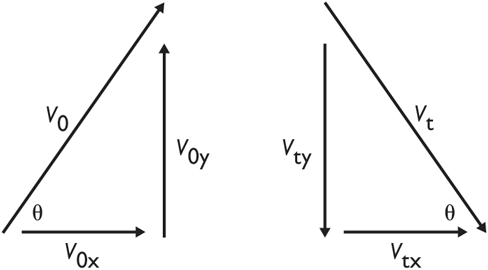
\includegraphics[width=\maxwidth,height=\maxheight,keepaspectratio,alt={Image}]{Figures/img_p83_1.png}}
\end{center}


\caption{Image}
\end{figure}

\begin{verbatim}
double xVelocity = velocity * Math.cos(angle);
double yVelocity = velocity * Math.sin(angle);
\end{verbatim}

Bởi vì chúng ta đang bỏ qua khả năng có sức cản của không khí, vận tốc
theo phương \(x\) sẽ không thay đổi. Tuy nhiên, vận tốc theo phương
\(y\) lại chịu lực hút của trọng lực. Vật lý học cho chúng ta biết rằng
trên bề mặt Trái đất, gia tốc do trọng lực xấp xỉ
\(9.81\text{ meters/second}^2\). Đây là một giá trị thích hợp để định
nghĩa thành một hằng số của lớp (class constant):

\begin{verbatim}
public static final double ACCELERATION = -9.81;
\end{verbatim}

Lưu ý rằng chúng ta định nghĩa gia tốc trọng lực là một số âm bởi vì nó
làm giảm vận tốc theo phương \(y\) của một vật thể (kéo nó xuống thay vì
đẩy nó lên).

Mục tiêu của chúng ta là hiển thị các giá trị \(x\), \(y\) và thời gian
trôi qua khi vật thể bay lên và sau đó rơi xuống. Vận tốc theo phương
\(y\) giảm dần cho đến khi nó bằng \(0\). Từ vật lý học, chúng ta biết
rằng đồ thị của vật thể sẽ đối xứng. Vật thể sẽ bay lên trên cho đến khi
vận tốc theo phương \(y\) của nó đạt tới \(0\), và sau đó nó sẽ theo một
đường đi tương tự rơi trở xuống trong một khoảng thời gian bằng nhau. Do
đó, tổng thời gian tính bằng giây có thể được tính như sau:

\begin{verbatim}
double totalTime = -2.0 * yVelocity / ACCELERATION;
\end{verbatim}

Bây giờ, làm thế nào để chúng ta tính toán các giá trị của \(x\), \(y\)
và thời gian trôi qua để đưa vào bảng của chúng ta? Việc tính toán hai
trong số này là tương đối đơn giản. Chúng ta muốn có các khoảng gia số
thời gian (time increments) đều đặn cho mỗi mục nhập trong bảng, do đó
chúng ta có thể tính toán gia số thời gian bằng cách chia tổng thời gian
cho số bước chúng ta muốn đưa vào bảng của mình:

\begin{verbatim}
double timeIncrement = totalTime / steps;
\end{verbatim}

Như đã lưu ý ở trên, vận tốc theo phương \(x\) không thay đổi, vì vậy
đối với mỗi khoảng gia số thời gian này, chúng ta di chuyển cùng một
khoảng cách theo hướng \(x\):

\begin{verbatim}
double xIncrement = xVelocity * timeIncrement;
\end{verbatim}

Giá trị khó để tính toán ở đây là vị trí \(y\). Vì gia tốc do trọng lực,
vận tốc theo phương \(y\) thay đổi theo thời gian. Nhưng từ vật lý học,
chúng ta có công thức tổng quát sau để tính toán độ dời (displacement)
của một vật thể với vận tốc \(v\), thời gian \(t\) và gia tốc \(a\):

\(displacement = v t + \frac{1}{2} a t^2\)

Trong trường hợp của chúng ta, vận tốc chúng ta muốn là vận tốc theo
phương \(y\) và gia tốc là từ hằng số trọng lực của Trái đất. Do đó, đây
là một mô tả bằng mã giả (pseudocode) về cách tạo ra bảng:

\begin{verbatim}
thiết lập tất cả x, y, và t bằng 0.
for (số bước đã cho) {
    cộng thêm timeIncrement vào t.
    cộng thêm xIncrement vào x.
    đặt lại y thành yVelocity * t + 0.5 * ACCELERATION * t * t.
    báo cáo số bước (step #), x, y, t.
}
\end{verbatim}

Chúng ta đã khá gần với việc có mã Java thực sự ở đây, nhưng chúng ta
phải suy nghĩ về cách báo cáo các giá trị của \(x\), \(y\) và \(t\)
trong một bảng. Chúng đều sẽ có kiểu \texttt{double}, điều đó có nghĩa
là chúng có khả năng tạo ra một lượng lớn các chữ số sau dấu thập phân.
Nhưng chúng ta không muốn nhìn thấy tất cả các chữ số đó, vì chúng không
đặc biệt liên quan và vì các tính toán của chúng ta không chính xác đến
mức đó.

Trước khi chúng ta cố gắng hoàn thành đoạn mã cho bảng, hãy nghĩ về vấn
đề hiển thị chỉ một số chữ số của một số. Ý tưởng là cắt bớt (truncate)
các chữ số để chúng ta không nhìn thấy tất cả chúng. Một cách để cắt bớt
là ép kiểu một số \texttt{double} thành một số \texttt{int}, thao tác
này sẽ cắt bớt tất cả các chữ số sau dấu thập phân. Chúng ta có thể làm
điều đó, nhưng chúng ta có lẽ muốn giữ lại ít nhất một số chữ số trong
đó. Ví dụ, giả sử rằng chúng ta muốn báo cáo hai chữ số sau dấu thập
phân. Thủ thuật (trick) ở đây là đưa hai chữ số mà chúng ta muốn sang
phía bên kia của dấu thập phân. Chúng ta có thể làm điều đó bằng cách
nhân với 100 và sau đó ép kiểu sang \texttt{int}:

\begin{verbatim}
(int) (n * 100.0)
\end{verbatim}

Biểu thức này mang lại cho chúng ta các chữ số mà chúng ta muốn, nhưng
bây giờ dấu thập phân nằm sai chỗ. Ví dụ, nếu \(n\) ban đầu là
\(3.488834\), biểu thức trên sẽ cho chúng ta \(348\). Chúng ta phải chia
kết quả này cho 100 để biến nó trở lại thành số \(3.48\):

\begin{verbatim}
(int) (n * 100.0) / 100.0
\end{verbatim}

Trong khi đang làm việc này, chúng ta có thể thực hiện một cải tiến cuối
cùng. Lưu ý rằng số ban đầu là \(3.488834\). Nếu chúng ta cắt bớt đơn
giản, chúng ta nhận được \(3.48\), nhưng thực sự số này gần với \(3.49\)
hơn. Chúng ta có thể làm tròn đến chữ số gần nhất bằng cách gọi phương
thức \texttt{Math.round} trên số đó thay vì ép kiểu nó:

\begin{verbatim}
Math.round(n * 100.0) / 100.0
\end{verbatim}

Đây là một thao tác mà chúng ta có khả năng sẽ muốn thực hiện trên nhiều
hơn một con số, vì vậy nó xứng đáng được đưa vào trong một phương thức:

\begin{verbatim}
public static double round2(double n) {
    return Math.round(n * 100.0) / 100.0;
}
\end{verbatim}

Quay trở lại mã giả của chúng ta cho bảng, chúng ta có thể kết hợp các
lời gọi tới phương thức \texttt{round2} để tiến gần hơn một chút tới mã
Java thực tế:

\begin{verbatim}
thiết lập tất cả x, y, và t bằng 0.
for (số bước đã cho) {
    cộng thêm timeIncrement vào t.
    cộng thêm xIncrement vào x.
    đặt lại y thành yVelocity * t + 0.5 * ACCELERATION * t * t.
    báo cáo số bước (step #), round2(x), round2(y), round2(t).
}
\end{verbatim}

Sẽ rất tuyệt nếu các giá trị trong bảng được căn chỉnh. Để có được các
con số xếp thành hàng ngay ngắn, chúng ta sẽ phải sử dụng đầu ra có định
dạng (formatted output), điều mà chúng ta sẽ thảo luận trong Chương 4.
Hiện tại, chúng ta ít nhất có thể sắp xếp các con số thành các cột bằng
cách tách chúng bằng các ký tự tab. Hãy nhớ rằng trình tự thoát (escape
sequence) \texttt{\textbackslash{}t} đại diện cho một dấu tab duy nhất.

Nếu chúng ta định có một bảng với các cột, việc có một tiêu đề (header)
cho bảng cũng rất hợp lý. Và chúng ta có lẽ muốn đưa vào một dòng trong
bảng hiển thị điều kiện ban đầu, nơi \(x\), \(y\) và \(time\) đều bằng
\(0\). Do đó, chúng ta có thể mở rộng mã giả của mình thành mã Java sau:

\begin{verbatim}
double x = 0.0;
double y = 0.0;
double t = 0.0;
System.out.println("step\tx\ty\ttime");
System.out.println("0\t0.0\t0.0\t0.0");
for (int i = 1; i <= steps; i++) {
    t += timeIncrement;
    x += xIncrement;
    y = yVelocity * t + 0.5 * ACCELERATION * t * t;
    System.out.println(i + "\t" + round2(x) + "\t" +
                       round2(y) + "\t" + round2(t));
}
\end{verbatim}

\subsubsection{Giải pháp Không có Cấu trúc (Unstructured
Solution)}\label{giux1ea3i-phuxe1p-khuxf4ng-cuxf3-cux1ea5u-truxfac-unstructured-solution}

Chúng ta có thể ghép tất cả các phần này lại với nhau để tạo thành một
chương trình hoàn chỉnh. Trước tiên, hãy xem một phiên bản không có cấu
trúc bao gồm phần lớn mã trong phương thức \texttt{main}. Phiên bản này
cũng bao gồm một số câu lệnh \texttt{println} mới ở phần đầu để giới
thiệu ngắn gọn cho người dùng:

\begin{verbatim}
 1  // This program computes the trajectory of a projectile.
 2
 3  import java.util.*; // for Scanner
 4
\end{verbatim}

\begin{verbatim}
 5  public class Projectile {
 6      // constant for Earth acceleration in meters/second^2
 7      public static final double ACCELERATION = -9.81;
 8
 9      public static void main(String[] args) {
 10         Scanner console = new Scanner(System.in);
 11
 12         System.out.println("This program computes the");
 13         System.out.println("trajectory of a projectile given");
 14         System.out.println("its initial velocity and its");
 15         System.out.println("angle relative to the");
 16         System.out.println("horizontal.");
 17         System.out.println();
 18
 19         System.out.print("velocity (meters/second)? ");
 20         double velocity = console.nextDouble();
 21         System.out.print("angle (degrees)? ");
 22         double angle = Math.toRadians(console.nextDouble());
 23         System.out.print("number of steps to display? ");
 24         int steps = console.nextInt();
 25         System.out.println();
 26
 27         double xVelocity = velocity * Math.cos(angle);
 28         double yVelocity = velocity * Math.sin(angle);
 29         double totalTime = -2.0 * yVelocity / ACCELERATION;
 30         double timeIncrement = totalTime / steps;
 31         double xIncrement = xVelocity * timeIncrement;
 32
 33         double x = 0.0;
 34         double y = 0.0;
 35         double t = 0.0;
 36         System.out.println("step\tx\ty\ttime");
 37         System.out.println("0\t0.0\t0.0\t0.0");
 38         for (int i = 1; i <= steps; i++) {
 39             t += timeIncrement;
 40             x += xIncrement;
 41             y = yVelocity * t + 0.5 * ACCELERATION * t * t;
 42             System.out.println(i + "\t" + round2(x) + "\t" +
 43                                round2(y) + "\t" + round2(t));
 44         }
 45     }
 46
 47     public static double round2(double n) {
 48         return Math.round(n * 100.0) / 100.0;
 49     }
 50 }
\end{verbatim}

Dưới đây là một quá trình thực thi mẫu của chương trình:

\begin{verbatim}
This program computes the 
trajectory of a projectile given 
its initial velocity and its 
angle relative to the 
horizontal. 
velocity (meters/second)? 30  
angle (degrees)? 50  
number of steps to display? 10  
step    x        y        time 
0       0.0      0.0      0.0 
1       9.03     9.69     0.47 
2       18.07    17.23    0.94 
3       27.1     22.61    1.41 
4       36.14    25.84    1.87 
5       45.17    26.92    2.34 
6       54.21    25.84    2.81 
7       63.24    22.61    3.28 
8       72.28    17.23    3.75 
9       81.31    9.69     4.22 
10      90.35    0.0      4.69
\end{verbatim}

Từ nhật ký thực thi, bạn có thể thấy rằng vật thể đạt đến chiều cao tối
đa là 26.92 mét sau 2.34 giây (bước thứ năm) và nó rơi cách điểm xuất
phát 90.35 mét sau 4.69 giây (bước thứ mười).

Phiên bản này của chương trình hoạt động, nhưng chúng ta thường không
muốn đưa quá nhiều mã vào phương thức \texttt{main}. Phần tiếp theo sẽ
khám phá cách chia nhỏ chương trình thành các phần nhỏ hơn.

\subsubsection{Giải pháp Cấu trúc (Structured
Solution)}\label{giux1ea3i-phuxe1p-cux1ea5u-truxfac-structured-solution}

Có ba khối mã chính trong phương thức \texttt{main} của chương trình
\texttt{Projectile}: một chuỗi các câu lệnh \texttt{println} giới thiệu
chương trình cho người dùng, một chuỗi các câu lệnh nhắc người dùng nhập
ba giá trị được sử dụng để tạo bảng, và sau đó là mã tạo ra chính cái
bảng đó.

Do đó, trong mã giả, cấu trúc tổng thể trông giống như thế này:

\begin{verbatim}
đưa ra giới thiệu.
nhắc nhập vận tốc, góc, và số bước.
tạo ra bảng.
\end{verbatim}

Bước thứ nhất và bước thứ ba dễ dàng được chuyển thành các phương thức,
nhưng bước ở giữa thì không. Bước này nhắc người dùng nhập các giá trị
mà chúng ta cần để tạo ra bảng. Nếu chúng ta chuyển nó thành một phương
thức, nó sẽ phải bằng cách nào đó trả về ba giá trị lại cho
\texttt{main}. Một phương thức chỉ có thể trả về một giá trị duy nhất,
vì vậy thật không may chúng ta không thể chuyển bước này thành một
phương thức. Chúng ta có thể chuyển nó thành ba phương thức khác nhau,
một phương thức cho mỗi trong số ba giá trị, nhưng mỗi phương thức đó sẽ
chỉ dài hai dòng, vì vậy không rõ liệu làm như vậy có cải thiện cấu trúc
tổng thể hay không.

Do đó, cải tiến chính mà chúng ta có thể thực hiện là tách phần giới
thiệu và phần bảng thành các phương thức riêng biệt. Một cải tiến khác
mà chúng ta có thể thực hiện là biến công thức độ dời trong vật lý thành
phương thức của riêng nó. Việc biến các phương trình thành các phương
thức luôn là một ý tưởng hay. Đưa ra các phương thức đó, chúng ta có
phiên bản cấu trúc (structured version) sau đây của chương trình:

\begin{verbatim}
 1  // This program computes the trajectory of a projectile.
 2
 3  import java.util.*;     // for Scanner
 4
 5  public class Projectile2 {
 6      // constant for Earth acceleration in meters/second^2
 7      public static final double ACCELERATION = -9.81;
 8
 9      public static void main(String[] args) {
 10         Scanner console = new Scanner(System.in);
 11         giveIntro();
 12
 13         System.out.print("velocity (meters/second)? ");
 14         double velocity = console.nextDouble();
 15         System.out.print("angle (degrees)? ");
 16         double angle = Math.toRadians(console.nextDouble());
 17         System.out.print("number of steps to display? ");
 18         int steps = console.nextInt();
 19         System.out.println();
 20
\end{verbatim}

\begin{verbatim}
 21         printTable(velocity, angle, steps);
 22     }
 23
 24     // prints a table showing the trajectory of an object given
 25     // its initial velocity and angle and including the given
 26     // number of steps in the table
 27     public static void printTable(double velocity,
 28                                   double angle, int steps) {
 29         double xVelocity = velocity * Math.cos(angle);
 30         double yVelocity = velocity * Math.sin(angle);
 31         double totalTime = -2.0 * yVelocity / ACCELERATION;
 32         double timeIncrement = totalTime / steps;
 33         double xIncrement = xVelocity * timeIncrement;
 34
 35         double x = 0.0;
 36         double y = 0.0;
 37         double t = 0.0;
 38         System.out.println("step\tx\ty\ttime");
 39         System.out.println("0\t0.0\t0.0\t0.0");
 40         for (int i = 1; i <= steps; i++) {
 41             t += timeIncrement;
 42             x += xIncrement;
 43             y = displacement(yVelocity, t, ACCELERATION);
 44             System.out.println(i + "\t" + round2(x) + "\t" +
 45                                round2(y) + "\t" + round2(t));
 46         }
 47     }
 48
 49     // gives a brief introduction to the user
 50     public static void giveIntro() {
 51         System.out.println("This program computes the");
 52         System.out.println("trajectory of a projectile given");
 53         System.out.println("its initial velocity and its");
 54         System.out.println("angle relative to the");
 55         System.out.println("horizontal.");
 56         System.out.println();
 57     }
 58
 59     // returns the vertical displacement for a body given
 60     // initial velocity v, elapsed time t, and acceleration a
 61     public static double displacement(double v, double  t,
 62                                       double a){
 63         return  v * t + 0.5 * a * t * t;
 64     }
 65
 66     // rounds n to 2 digits after the decimal point
 67     public static double round2(double n) {
 68         return Math.round(n * 100.0) / 100.0;
 69     }
 70 }
\end{verbatim}

Phiên bản này thực thi theo cùng một cách như phiên bản trước đó.

\subsection{Tóm tắt Chương (Chapter
Summary)}\label{tuxf3m-tux1eaft-chux1b0ux1a1ng-chapter-summary}

Các phương thức có thể được viết để chấp nhận các tham số (parameters),
là tập hợp các đặc điểm phân biệt các thành viên khác nhau của một họ
các tác vụ. Các tham số cho phép các giá trị dữ liệu đi vào một phương
thức, điều này có thể thay đổi cách phương thức thực thi. Một phương
thức được khai báo với một tập hợp các tham số có thể thực hiện toàn bộ
một họ các tác vụ tương tự nhau thay vì chỉ một tác vụ duy nhất.

Khi các giá trị nguyên thủy như kiểu \texttt{int} hoặc \texttt{double}
được truyền vào như là các tham số, các giá trị của chúng được sao chép
vào phương thức. Các tham số nguyên thủy (primitive parameters) gửi các
giá trị vào một phương thức nhưng không gửi ra khỏi phương thức đó;
phương thức có thể sử dụng các giá trị dữ liệu nhưng không thể ảnh hưởng
đến giá trị của bất kỳ biến nào nằm ngoài nó.

Hai phương thức có thể có cùng tên nếu chúng khai báo các tham số khác
nhau. Điều này được gọi là nạp chồng (overloading).

Các phương thức có thể được viết để trả về các giá trị cho mã đang gọi
(calling code). Tính năng này cho phép một phương thức thực hiện một
phép tính phức tạp và sau đó cung cấp kết quả của nó trở lại cho mã đang
gọi. Kiểu của giá trị trả về phải được khai báo trong tiêu đề của phương
thức và được gọi là kiểu trả về (return type) của phương thức.

Java có một lớp tên là \texttt{Math} chứa một số phương thức tĩnh hữu
ích mà bạn có thể sử dụng trong các chương trình của mình, chẳng hạn như
lũy thừa, căn bậc hai, và logarit.

Một đối tượng (object) là một thực thể kết hợp dữ liệu và các thao tác.
Một số đối tượng trong Java bao gồm \texttt{String} (là chuỗi các ký tự
văn bản) và \texttt{Scanner} (chuyên đọc đầu vào của người dùng).

Các đối tượng chứa các phương thức hiện thực hóa các hành vi của chúng.
Để gọi một phương thức trên một đối tượng, hãy viết tên của đối tượng
đó, theo sau là một dấu chấm, theo sau là tên phương thức.

Một đối tượng \texttt{String} chứa một chuỗi các ký tự. Các ký tự có các
chỉ số (indexes), bắt đầu với \texttt{0} cho ký tự đầu tiên.

Ngoại lệ (exception) là một lỗi xảy ra khi một chương trình đã thực hiện
một hành động không hợp lệ và không thể tiếp tục thực thi bình thường.

Một số chương trình có tính tương tác và phản hồi đối với đầu vào từ
người dùng. Những chương trình này nên in một thông báo tới người dùng,
còn được gọi là lời nhắc (prompt), để yêu cầu nhập dữ liệu.

Java có một lớp tên là \texttt{Scanner} chuyên đọc đầu vào từ bàn phím.
Một đối tượng \texttt{Scanner} có thể đọc nhiều phần khác nhau của đầu
vào (còn được gọi là các thẻ bài) từ một nguồn đầu vào. Nó có thể đọc
từng thẻ bài một lần hoặc đọc toàn bộ một dòng tại một thời điểm.

\subsection{Bài tập Tự Kiểm tra (Self-Check
Problems)}\label{buxe0i-tux1eadp-tux1ef1-kiux1ec3m-tra-self-check-problems}

\subsubsection{Phần 3.1: Các Tham số
(Parameters)}\label{phux1ea7n-3.1-cuxe1c-tham-sux1ed1-parameters}

\textbf{1.} Cú pháp nào sau đây là chính xác cho một tiêu đề phương thức
có chứa các tham số?

\begin{enumerate}
\def\labelenumi{\alph{enumi}.}
\tightlist
\item
  \texttt{public\ static\ void\ example(x,\ y)\ \{}\strut \\
\item
  \texttt{public\ static\ (int\ x,\ int\ y)\ example()\ \{}\strut \\
\item
  \texttt{public\ static\ void\ example(int\ x,\ y)\ \{}\strut \\
\item
  \texttt{public\ static\ void\ example(x:\ int,\ y:\ int)\ \{}\strut \\
\item
  \texttt{public\ static\ void\ example(int\ x,\ int\ y)\ \{}
\end{enumerate}

\textbf{2.} Kết quả đầu ra do chương trình sau đây tạo ra là gì?

\begin{verbatim}
 1  public class MysteryNums {
 2      public static void main(String[] args) {
 3          int x = 15;
 4          sentence(x, 42);
 5
 6          int y = x - 5;
 7          sentence(y, x + y);
 8      }
 9
 10     public static void sentence(int num1, int num2) {
 11         System.out.println(num1 + " " + num2);
 12     }
 13  }
\end{verbatim}

\textbf{3.} Chương trình sau đây có 9 lỗi sai. Chúng là gì?

\begin{verbatim}
 1  public class Oops3 {
 2      public static void main() {
 3          double bubble = 867.5309;
 4          double x = 10.01;
 5          printer(double x, double y);
 6          printer(x);
 7          printer("barack", "obama");
 8          System.out.println("z = " + z);
 9      }
 10
 11     public static void printer(x, y double) {
 12         int z = 5;
 13         System.out.println("x = " + double x + " and y = " + y);
 14         System.out.println("The value from main is: " + bubble);
 15     }
 16  }
\end{verbatim}

\textbf{4.} Kết quả đầu ra do chương trình sau đây tạo ra là gì?

\begin{verbatim}
 1  public class Odds {
 2      public static void main(String[] args) {
 3          printOdds(3);
 4          printOdds(17 / 2);
 5
 6          int x = 25;
 7          printOdds(37 - x + 1);
 8      }
 9
 10     public static void printOdds(int n) {
 11         for (int i = 1; i <= n; i++) {
 12             int odd = 2 * i - 1;
 13             System.out.print(odd + " ");
 14         }
 15         System.out.println();
 16     }
 17  }
\end{verbatim}

\textbf{5.} Kết quả đầu ra của chương trình sau đây là gì?

\begin{verbatim}
 1   public class Weird {
 2      public static void main(String[] args) {
 3          int number = 8;
 4          halfTheFun(11);
 5          halfTheFun(2 - 3 + 2 * 8);
 6          halfTheFun(number);
 7          System.out.println("number = " + number);
 8      }
 9
 10     public static void halfTheFun(int number) {
 11         number = number / 2;
 12         for (int count = 1; count <= number; count++) {
\end{verbatim}

\begin{verbatim}
 13             System.out.print(count + " ");
 14         }
 15         System.out.println();
 16     }
 17  }
\end{verbatim}

\textbf{6.} Kết quả đầu ra của chương trình sau đây là gì?

\begin{verbatim}
 1  public class MysteryNumbers {
 2      public static void main(String[] args) {
 3          String one = "two";
 4          String two = "three";
 5          String three = "1";
 6          int number = 20;
 7
 8          sentence(one, two, 3);
 9          sentence(two, three, 14);
 10         sentence(three, three, number + 1);
 11         sentence(three, two, 1);
 12         sentence("eight", three, number / 2);
 13     }
 14
 15     public static void sentence(String three, String one, int number) {
 16         System.out.println(one + " times " + three + " = " + (number * 2));
 17     }
 18  }
\end{verbatim}

\textbf{7.} Kết quả đầu ra do chương trình sau đây tạo ra là gì?

\begin{verbatim}
 1  public class MysteryWho {
 2      public static void main(String[] args) {
 3          String whom = "her";
 4          String who = "him";
 5          String it = "who";
 6          String he = "it";
 7          String she = "whom";
 8
 9          sentence(he, she, it);
 10         sentence(she, he, who);
 11         sentence(who, she, who);
 12         sentence(it, "stu", "boo");
 13         sentence(it, whom, who);
 14     }
 15
 16     public static void sentence(String she, String who, String whom) {
 17         System.out.println(who + " and " + whom + " like " + she);
 18     }
 19  }
\end{verbatim}

\textbf{8.} Kết quả đầu ra do chương trình sau đây tạo ra là gì?

\begin{verbatim}
 1  public class MysteryTouch {
 2      public static void main(String[] args) {
 3          String head = "shoulders";
 4          String knees = "toes";
 5          String elbow = "head";
 6          String eye = "eyes and ears";
 7          String ear = "eye";
 8
 9          touch(ear, elbow);
 10         touch(elbow, ear);
 11         touch(head, "elbow");
 12         touch(eye, eye);
 13         touch(knees, "Toes");
 14         touch(head, "knees " + knees);
 15     }
 16
 17     public static void touch(String elbow, String ear) {
 18         System.out.println("touch your " + elbow + " to your " + ear);
 19     }
 20  }
\end{verbatim}

\textbf{9.} Kết quả đầu ra do chương trình sau đây tạo ra là gì?

\begin{verbatim}
 1  public class MysterySoda {
 2      public static void main(String[] args) {
 3          String soda = "Coke";
 4          String pop = "Pepsi";
 5          String Coke = "pop";
 6          String Pepsi = "soda";
 7          String say = pop;
 8
 9          carbonated(Coke, soda, pop);
 10         carbonated(pop, Pepsi, Pepsi);
 11         carbonated("pop", pop, "Kool-Aid");
 12         carbonated(say, "say", pop);
 13     }
 14
 15     public static void carbonated(String Coke, String soda, String pop) {
 16         System.out.println("say " + soda + " not " + pop + " or " + Coke);
 17     }
 18  }
\end{verbatim}

\textbf{10.} Viết một phương thức có tên là \texttt{printStrings} nhận
một tham số \texttt{String} và một tham số đại diện cho số lần lặp lại
và in ra \texttt{String} đó số lần đã cho với một khoảng trắng sau mỗi
lần. Ví dụ, lời gọi hàm

\begin{verbatim}
printStrings("abc", 5);
\end{verbatim}

sẽ in ra đầu ra sau:

\begin{verbatim}
abc abc abc abc abc
\end{verbatim}

\textbf{11.} Câu lệnh \texttt{System.out.println} hoạt động trên nhiều
kiểu giá trị khác nhau, chẳng hạn như số nguyên (integers) hoặc số thực
dấu phẩy động (doubles). Thuật ngữ dùng để gọi một phương thức như vậy
là gì?

\subsubsection{Phần 3.2: Các Phương thức Trả về Giá trị (Methods That
Return
Values)}\label{phux1ea7n-3.2-cuxe1c-phux1b0ux1a1ng-thux1ee9c-trux1ea3-vux1ec1-giuxe1-trux1ecb-methods-that-return-values}

\textbf{12.} Có gì sai với chương trình sau đây?

\begin{verbatim}
 1  public class Temperature {
 2      public static void main(String[] args) {
 3          double tempf = 98.6;
 4          double tempc = 0.0;
 5          ftoc(tempf, tempc);
 6          System.out.println("Body temp in C is: " + tempc);
 7      }
 8
 9      // converts Fahrenheit temperatures to Celsius
 10     public static void ftoc(double tempf, double tempc) {
 11         tempc = (tempf - 32) * 5 / 9;
 12     }
 13  }
\end{verbatim}

\textbf{13.} Đánh giá các biểu thức sau:

\begin{enumerate}
\def\labelenumi{\alph{enumi}.}
\tightlist
\item
  \texttt{Math.abs(-1.6)}\strut \\
\item
  \texttt{Math.abs(2\ +\ -4)}\strut \\
\item
  \texttt{Math.pow(6,\ 2)}\strut \\
\item
  \texttt{Math.pow(5\ /\ 2,\ 6)}\strut \\
\item
  \texttt{Math.ceil(9.1)}\strut \\
\item
  \texttt{Math.ceil(115.8)}\strut \\
\item
  \texttt{Math.max(7,\ 4)}\strut \\
\item
  \texttt{Math.min(8,\ 3\ +\ 2)}\strut \\
\item
  \texttt{Math.min(-2,\ -5)}\strut \\
\item
  \texttt{Math.sqrt(64)}\strut \\
\item
  \texttt{Math.sqrt(76\ +\ 45)}\strut \\
\item
  \texttt{100\ +\ Math.log10(100)}\strut \\
\item
  \texttt{13\ +\ Math.abs(-7)\ -\ Math.pow(2,\ 3)\ +\ 5}\strut \\
\item
  \texttt{Math.sqrt(16)\ *\ Math.max(Math.abs(-5),\ Math.abs(-3))}\strut \\
\item
  \texttt{7\ -\ 2\ +\ Math.log10(1000)\ +\ Math.log(Math.pow(Math.E,\ 5))}\strut \\
\item
  \texttt{Math.max(18\ -\ 5,\ Math.ceil(4.6\ *\ 3))}
\end{enumerate}

\textbf{14.} Kết quả đầu ra do chương trình sau đây tạo ra là gì?

\begin{verbatim}
 1  public class MysteryReturn {
 2      public static void main(String[] args) {
 3          int x = 1, y = 2, z = 3;
 4          z = mystery(x, z, y);
 5          System.out.println(x + " " + y + " " + z);
 6          x = mystery(z, z, x);
 7          System.out.println(x + " " + y + " " + z);
 8          y = mystery(y, y, z);
 9          System.out.println(x + " " + y + " " + z);
 10     }
 11
 12     public static int mystery(int z, int x, int y) {
 13         z--;
 14         x = 2 * y + z;
 15         y = x - 1;
 16         System.out.println(y + " " + z);
 17         return x;
 18     }
 19  }
\end{verbatim}

\textbf{15.} Viết kết quả của từng biểu thức. Lưu ý rằng giá trị của một
biến chỉ thay đổi nếu bạn gán lại nó bằng cách sử dụng toán tử
\texttt{=}.

\begin{verbatim}
double grade = 2.7;
Math.round(grade);                                // grade =
grade = Math.round(grade);                        // grade =
double min = Math.min(grade, Math.floor(2.9));    // min =
double x = Math.pow(2, 4);                        // x =
x = Math.sqrt(64);                                // x =
int count = 25;
Math.sqrt(count);                                 // count =
count = (int) Math.sqrt(count);                   // count =
int a = Math.abs(Math.min(-1, -3));               // a =
\end{verbatim}

\textbf{16.} Viết một phương thức có tên là \texttt{min} nhận ba số
nguyên làm tham số và trả về giá trị nhỏ nhất trong ba giá trị; ví dụ:
một lời gọi \texttt{min(3,\ -2,\ 7)} sẽ trả về \texttt{-2}, và một lời
gọi \texttt{min(19,\ 27,\ 6)} sẽ trả về \texttt{6}. Sử dụng
\texttt{Math.min} để viết giải pháp của bạn.

\textbf{17.} Viết một phương thức có tên là \texttt{countQuarters} nhận
một tham số \texttt{int} đại diện cho một số xu (cents) và trả về số
lượng đồng 25 xu (quarter coins) được biểu diễn bởi ngần ấy số xu. Không
đếm bất kỳ đô la chẵn nào, bởi vì chúng sẽ được phân phát dưới dạng các
tờ đô la. Ví dụ: \texttt{countQuarters(64)} sẽ trả về \texttt{2}, vì
\texttt{64} xu tương đương với \texttt{2} đồng 25 xu và còn dư
\texttt{14} xu. Một lời gọi \texttt{countQuarters(1278)} sẽ trả về
\texttt{3}, bởi vì sau khi lấy đi \texttt{12} đô la, còn lại \texttt{3}
đồng 25 xu nằm trong \texttt{78} xu còn dư đó.

\subsubsection{Phần 3.3: Sử dụng các Đối tượng (Using
Objects)}\label{phux1ea7n-3.3-sux1eed-dux1ee5ng-cuxe1c-ux111ux1ed1i-tux1b0ux1ee3ng-using-objects}

\textbf{18.} Kết quả đầu ra do đoạn mã sau đây tạo ra là gì?

\begin{verbatim}
String first = "James";
String last = "Kirk";
String middle = "T.";
System.out.println(last);
System.out.println("My name is " + first);
System.out.println(first + " " + last);
System.out.println(last + ", " + first + " " + middle);
System.out.println(middle + " is for Tiberius");
\end{verbatim}

\textbf{19.} Giả sử rằng các biến sau đã được khai báo:

\begin{verbatim}
//       index 0123456789012345
String str1 = "Frodo Baggins";
String str2 = "Gandalf the GRAY";
\end{verbatim}

đánh giá các biểu thức sau:

\begin{enumerate}
\def\labelenumi{\alph{enumi}.}
\item
  \texttt{str1.length()}\strut \\
\item
  \texttt{str1.charAt(7)}\strut \\
\item
  \texttt{str2.charAt(0)}\strut \\
\item
  \texttt{str1.indexOf("o")}\strut \\
\item
  \texttt{str2.toUpperCase()}\strut \\
\item
  \texttt{str1.toLowerCase().indexOf("B")}
\item
  \texttt{str1.substring(4)}\strut \\
\item
  \texttt{str2.substring(3,\ 14)}\strut \\
\item
  \texttt{str2.replace("a",\ "oo")}\strut \\
\item
  \texttt{str2.replace("gray",\ "white")}\strut \\
\item
  \texttt{"str1".replace("r",\ "range")}
\end{enumerate}

\textbf{20.} Giả sử rằng các biến sau đã được khai báo:

\begin{verbatim}
String str1 = "Q.E.D.";
String str2 = "Arcturan Megadonkey";
String str3 = "Sirius Cybernetics Corporation";
\end{verbatim}

đánh giá các biểu thức sau:

\begin{enumerate}
\def\labelenumi{\alph{enumi}.}
\tightlist
\item
  \texttt{str1.length()}\strut \\
\item
  \texttt{str2.length()}\strut \\
\item
  \texttt{str1.toLowerCase()}\strut \\
\item
  \texttt{str2.toUpperCase()}\strut \\
\item
  \texttt{str1.substring(2,\ 4)}\strut \\
\item
  \texttt{str2.substring(10,\ 14)}\strut \\
\item
  \texttt{str1.indexOf("D")}\strut \\
\item
  \texttt{str1.indexOf(".")}\strut \\
\item
  \texttt{str2.indexOf("donkey")}\strut \\
\item
  \texttt{str3.indexOf("X")}\strut \\
\item
  \texttt{str2\ +\ str3.charAt(17)}\strut \\
\item
  \texttt{str3.substring(9,\ str3.indexOf("e"))}\strut \\
\item
  \texttt{str3.substring(7,\ 12)}\strut \\
\item
  \texttt{str2.toLowerCase().substring(9,\ 13)\ +\ str3.substring(18,\ str3.length()\ -\ 7)}
\end{enumerate}

\textbf{21.} Xem xét \texttt{String} sau:

\begin{verbatim}
String quote = "Four score and seven years ago";
\end{verbatim}

Biểu thức nào tạo ra một \texttt{String} mới là \texttt{"SCORE"}? Biểu
thức nào tạo ra \texttt{"four\ years"}?

\textbf{22.} Xem xét đoạn mã sau:

\begin{verbatim}
Scanner console = new Scanner(System.in);
System.out.print("How much money do you have? ");
double money = console.nextDouble();
\end{verbatim}

Hãy mô tả những gì sẽ xảy ra khi người dùng gõ từng giá trị sau. Nếu mã
chạy thành công, hãy mô tả giá trị sẽ được lưu trữ trong biến
\texttt{money}.

\begin{enumerate}
\def\labelenumi{\alph{enumi}.}
\tightlist
\item
  \texttt{34.50}\strut \\
\item
  \texttt{6}\strut \\
\item
  \texttt{\$25.00}\strut \\
\item
  \texttt{million}\strut \\
\item
  \texttt{100*5}\strut \\
\item
  \texttt{600x000}\strut \\
\item
  \texttt{none}\strut \\
\item
  \texttt{645}
\end{enumerate}

Những lời gọi này sẽ tạo ra đầu ra sau:

\begin{verbatim}
1 2 4 8
1 2 4 8 16 32 64 128 256 512 1024
\end{verbatim}

Bạn có thể cho rằng giá trị được truyền vào \texttt{printPowersOf2} là
\texttt{0} hoặc lớn hơn. (Lớp \texttt{Math} có thể giúp bạn giải quyết
bài toán này. Nếu bạn sử dụng nó, bạn có thể cần ép kiểu (cast) các kết
quả của nó từ \texttt{double} sang \texttt{int} để bạn không nhìn thấy
một \texttt{.0} sau mỗi số trong đầu ra của mình. Đồng thời hãy thử viết
chương trình này mà không sử dụng lớp \texttt{Math}.)

\textbf{3.} Viết một phương thức có tên là \texttt{printPowersOfN} nhận
một tham số cơ số (base) và một tham số số mũ (exponent) làm các đối số
và in ra mỗi lũy thừa của cơ số đó từ \(base^0\) (1) lên đến lũy thừa
tối đa đó, bao gồm cả giá trị đó. Ví dụ, hãy xem xét các lời gọi sau:

\begin{verbatim}
printPowersOfN(4, 3);
printPowersOfN(5, 6);
printPowersOfN(-2, 8);
\end{verbatim}

Những lời gọi này sẽ tạo ra đầu ra sau:

\begin{verbatim}
1 4 16 64
1 5 25 125 625 3125 15625
1 -2 4 -8 16 -32 64 -128 256
\end{verbatim}

Bạn có thể cho rằng số mũ được truyền vào \texttt{printPowersOfN} có giá
trị từ \texttt{0} trở lên. (Lớp \texttt{Math} có thể giúp bạn giải quyết
bài toán này. Nếu bạn sử dụng nó, bạn có thể cần ép kiểu các kết quả của
nó từ \texttt{double} sang \texttt{int} để bạn không nhìn thấy một
\texttt{.0} sau mỗi số trong đầu ra của mình. Đồng thời hãy thử viết
chương trình này mà không sử dụng lớp \texttt{Math}.)

\textbf{4.} Viết một phương thức có tên là \texttt{printSquare} nhận một
số nguyên nhỏ nhất (minimum) và lớn nhất (maximum) và in ra một hình
vuông chứa các dòng số tăng dần. Dòng đầu tiên sẽ bắt đầu bằng số nhỏ
nhất, và mỗi dòng tiếp theo sẽ bắt đầu bằng số cao hơn kế tiếp. Dãy số
trên một dòng sẽ vòng ngược (wraps back) trở lại số nhỏ nhất sau khi nó
chạm đến số lớn nhất. Ví dụ, lời gọi

\begin{verbatim}
printSquare(3, 7);
\end{verbatim}

sẽ tạo ra đầu ra sau:

\begin{verbatim}
34567
45673
56734
67345
73456
\end{verbatim}

Nếu số lớn nhất được truyền vào nhỏ hơn số nhỏ nhất, phương thức này
không tạo ra đầu ra nào.

\textbf{5.} Viết một phương thức có tên là \texttt{printGrid} nhận hai
số nguyên đại diện cho số hàng và số cột, và in ra một lưới (grid) các
số nguyên từ \(1\) đến \((rows \times columns)\) theo thứ tự ưu tiên cột
(column major order). Ví dụ, lời gọi

\begin{verbatim}
printGrid(4, 6);
\end{verbatim}

sẽ tạo ra đầu ra sau:

\begin{verbatim}
1 5 9 13 17 21
2 6 10 14 18 22
3 7 11 15 19 23
4 8 12 16 20 24
\end{verbatim}

\textbf{6.} Viết một phương thức có tên là \texttt{largerAbsVal} nhận
hai số nguyên làm các tham số và trả về giá trị lớn hơn trong hai giá
trị tuyệt đối. Một lời gọi \texttt{largerAbsVal(11,\ 2)} sẽ trả về
\texttt{11}, và một lời gọi \texttt{largerAbsVal(4,\ -5)} sẽ trả về
\texttt{5}.

\textbf{7.} Viết một biến thể của phương thức \texttt{largestAbsVal} từ
bài tập trước, phương thức này nhận ba số nguyên làm các tham số và trả
về giá trị lớn nhất trong ba giá trị tuyệt đối của chúng. Ví dụ, một lời
gọi \texttt{largestAbsVal(7,\ -2,\ -11)} sẽ trả về \texttt{11}, và một
lời gọi \texttt{largestAbsVal(-4,\ 5,\ 2)} sẽ trả về \texttt{5}.

\textbf{8.} Viết một phương thức có tên là \texttt{quadratic} giải các
phương trình bậc hai và in ra các nghiệm của chúng. Nhắc lại rằng phương
trình bậc hai là một phương trình đa thức với một biến \(x\) có dạng
\(ax^2 + bx + c = 0\). Công thức để giải phương trình bậc hai là:

\(x = \frac{-b \pm \sqrt{b^2 - 4ac}}{2a}\)

Dưới đây là một số phương trình ví dụ và các nghiệm của chúng:
\(x^2 - 7x + 12 = 0 : x = 4, x = 3\)
\(x^2 - 3x + 2 = 0 : x = -2, x = -1\)

Phương thức của bạn nên chấp nhận các hệ số \(a\), \(b\), và \(c\) làm
các tham số và nên in ra các nghiệm của phương trình. Bạn có thể giả
định rằng phương trình có hai nghiệm thực, mặc dù về mặt toán học điều
này không phải lúc nào cũng đúng.

\textbf{9.} Viết một phương thức có tên là \texttt{lastDigit} trả về chữ
số cuối cùng của một số nguyên. Ví dụ, \texttt{lastDigit(3572)} sẽ trả
về \texttt{2}. Nó cũng nên hoạt động cho cả số âm. Ví dụ,
\texttt{lastDigit(-947)} sẽ trả về \texttt{7}.

\textbf{10.} Viết một phương thức có tên là \texttt{area} chấp nhận bán
kính của một hình tròn làm tham số và trả về diện tích của hình tròn đó.
Ví dụ, lời gọi \texttt{area(2.0)} sẽ trả về \texttt{12.566370614359172}.
Nhắc lại rằng diện tích có thể được tính bằng số pi (\(\pi\)) nhân với
bình phương bán kính và Java có một hằng số có tên là \texttt{Math.PI}.

\textbf{11.} Viết một phương thức có tên là \texttt{distance} chấp nhận
bốn tọa độ nguyên \((x_1, y_1)\) và \((x_2, y_2)\) làm các tham số và
tính toán khoảng cách giữa các điểm \((x_1, y_1)\) và \((x_2, y_2)\)
trên mặt phẳng Descartes. Công thức tính khoảng cách là:

\(d = \sqrt{(x_2 - x_1)^2 + (y_2 - y_1)^2}\)

Ví dụ, lời gọi \texttt{distance(1,\ 0,\ 4,\ 4)} sẽ trả về \texttt{5.0}
và lời gọi \texttt{distance(10,\ 2,\ 3,\ 15)} sẽ trả về
\texttt{14.7648230602334}.

\textbf{12.} Viết một phương thức có tên là \texttt{scientific} chấp
nhận một cơ số là số thực và một số mũ làm các tham số và tính toán cơ
số nhân với 10 lũy thừa số mũ, như được thấy trong ký hiệu khoa học
(scientific notation). Ví dụ, lời gọi \texttt{scientific(6.23,\ 5)} sẽ
trả về \texttt{623000.0} và lời gọi \texttt{scientific(1.9,\ -2)} sẽ trả
về \texttt{0.019}.

\textbf{13.} Viết một phương thức có tên là \texttt{pay} nhận hai tham
số: một số thực cho mức lương của một trợ giảng (TA), và một số nguyên
cho số giờ trợ giảng đó đã làm việc trong tuần này. Phương thức này nên
trả về số tiền phải trả cho trợ giảng. Ví dụ, lời gọi
\texttt{pay(5.50,\ 6)} sẽ trả về \texttt{33.0}. Trợ giảng sẽ nhận được
lương ``làm thêm giờ'' bằng \(1\frac{1}{2}\) lần mức lương bình thường
cho bất kỳ số giờ nào vượt quá 8. Ví dụ, lời gọi \texttt{pay(4.00,\ 11)}
sẽ trả về \((4.00 \times 8) + (6.00 \times 3)\) hay \texttt{50.0}.

\textbf{14.} Viết một phương thức có tên là \texttt{cylinderSurfaceArea}
chấp nhận bán kính \(r\) và chiều cao \(h\) làm tham số và trả về diện
tích bề mặt của một hình trụ với các kích thước đó. Ví dụ, lời gọi
\texttt{cylinderSurfaceArea(3.0,\ 4.5)} sẽ trả về
\texttt{141.3716694115407}. Công thức tính diện tích bề mặt của một hình
trụ có bán kính \(r\) và chiều cao \(h\) là như sau:

\textbf{15.} Viết một phương thức có tên là \texttt{sphereVolume} chấp
nhận một bán kính làm tham số và trả về thể tích của một hình cầu có bán
kính đó. Ví dụ, lời gọi \texttt{sphereVolume(2.0)} sẽ trả về
\texttt{33.510321638291124}. Công thức tính thể tích của một hình cầu có
bán kính \(r\) là như sau: \(volume = \frac{4}{3}\pi r^3\)

\textbf{16.} Viết một phương thức có tên là \texttt{triangleArea} chấp
nhận ba độ dài cạnh của một tam giác làm các tham số và trả về diện tích
của một tam giác có các độ dài cạnh đó. Ví dụ, lời gọi
\texttt{triangleArea(8,\ 5.2,\ 7.1)} sẽ trả về
\texttt{18.151176098258745}. Để tính diện tích, hãy sử dụng công thức
Heron, phát biểu rằng diện tích của một tam giác có ba cạnh có độ dài
\(a\), \(b\), và \(c\) là công thức sau đây. Công thức này dựa trên giá
trị được tính toán \(s\), một chiều dài bằng một nửa chu vi của tam
giác: \(s = \frac{a + b + c}{2}\)
\(area = \sqrt{s(s - a)(s - b)(s - c)}\)

\textbf{17.} Viết một phương thức có tên là \texttt{padString} nhận hai
tham số: một chuỗi và một số nguyên đại diện cho độ dài. Phương thức này
sẽ thêm các khoảng trắng (pad) vào chuỗi tham số cho đến khi độ dài của
nó bằng với độ dài cho trước. Ví dụ, \texttt{padString("hello",\ 8)} sẽ
trả về \texttt{"hello\ \ \ "}. (Loại phương thức này hữu ích khi cố gắng
in đầu ra thẳng hàng theo chiều ngang.) Nếu độ dài của chuỗi đã dài ít
nhất bằng tham số độ dài, phương thức của bạn sẽ trả về chuỗi ban đầu.
Ví dụ, \texttt{padString("congratulations",\ 10)} sẽ trả về
\texttt{"congratulations"}.

\textbf{18.} Viết một phương thức có tên là \texttt{vertical} nhận một
chuỗi làm tham số của nó và in ra mỗi chữ cái của chuỗi trên các dòng
riêng biệt. Ví dụ, một lời gọi \texttt{vertical("hey\ now")} sẽ tạo ra
đầu ra sau:

\begin{verbatim}
h
e
y
 
n
o
w
\end{verbatim}

\textbf{19.} Viết một phương thức có tên là \texttt{printReverse} nhận
một chuỗi làm tham số của nó và in các ký tự theo thứ tự ngược lại. Ví
dụ, một lời gọi \texttt{printReverse("hello\ there!")} sẽ in ra
\texttt{"!ereht\ olleh"}. Nếu chuỗi rỗng được truyền vào, phương thức
này không tạo ra đầu ra nào.

\textbf{20.} Viết một phương thức có tên là \texttt{inputBirthday} chấp
nhận một đối tượng \texttt{Scanner} cho giao diện điều khiển (console)
làm tham số và nhắc người dùng nhập vào tháng, ngày và năm sinh, sau đó
in ngày sinh ra theo một định dạng phù hợp. Dưới đây là một ví dụ hội
thoại với người dùng:

\begin{verbatim}
On what day of the month were you born? 8
What is the name of the month in which you were born? May
During what year were you born? 1981
You were born on May 8, 1981. You’re mighty old!
\end{verbatim}

\textbf{21.} Viết một phương thức có tên là \texttt{processName} chấp
nhận một đối tượng \texttt{Scanner} cho giao diện điều khiển (console)
làm tham số và nhắc người dùng nhập vào họ và tên đầy đủ, sau đó in tên
theo thứ tự ngược lại (tức là, họ, tên). Dưới đây là một ví dụ hội thoại
với người dùng:

\begin{verbatim}
Please enter your full name: Sammy Jankis
Your name in reverse order is Jankis, Sammy
\end{verbatim}

\textbf{22.} Viết một chương trình xuất ra ``The Name Game'', trong đó
người dùng nhập tên (first name) và họ (last name) và một bài hát sẽ
được in ra về tên, rồi đến họ của họ. Sử dụng một phương thức để tránh
dư thừa (redundancy).

\textbf{23.} Viết một phương thức có tên là \texttt{printIndexed} nhận
một chuỗi làm tham số của nó và in ra các ký tự của chuỗi theo thứ tự
kèm theo chỉ số của chúng theo thứ tự ngược lại. Ví dụ, lời gọi
\texttt{printIndexed("ZELDA")} sẽ in \texttt{Z4E3L2D1A0} ra giao diện
điều khiển.

\subsubsection{Dự án lập trình (Programming
Projects)}\label{dux1ef1-uxe1n-lux1eadp-truxecnh-programming-projects}

\textbf{1.} Viết một chương trình tạo ra các hình ảnh của những cây
thông Noel làm đầu ra. Nó nên có một phương thức với hai tham số: một
cho số lượng các phân đoạn (segments) trong cây và một cho chiều cao của
mỗi phân đoạn. Ví dụ, cây được hiển thị ở đây bên trái có ba phân đoạn
với chiều cao là 4 và cây bên phải có hai phân đoạn với chiều cao là 5:

\begin{verbatim}
      *            *
     ***          ***
    *****        *****
   *******      *******
     ***       *********
    *****         ***
   *******       *****
  *********     *******
    *****      *********
   *******    ***********
  *********        *
 ***********       *
      *         *******
      *
   *******
\end{verbatim}

\textbf{2.} Một ngân hàng nhất định cung cấp lãi suất 6.5\% cho các tài
khoản tiết kiệm, được tính gộp (compounded) hàng năm. Hãy tạo một bảng
cho thấy số tiền mà một người sẽ tích lũy được trong một khoảng thời
gian 25 năm, giả sử rằng người đó thực hiện khoản đầu tư ban đầu là
\$1000 và gửi \$100 mỗi năm sau năm đầu tiên. Bảng của bạn nên chỉ ra số
dư hiện tại, tiền lãi, khoản tiền gửi mới và số dư mới cho mỗi năm.

\textbf{3.} Viết một chương trình cho thấy tổng số lượng quà tặng mà
người trong bài hát ``The Twelve Days of Christmas'' nhận được vào mỗi
ngày, như được chỉ ra trong Bảng 3.5.

Bảng 3.5 Mười hai ngày Giáng sinh

\textbf{4.} Viết một chương trình nhắc người dùng nhập vào độ dài các
cạnh của một tam giác và báo cáo ba góc của nó.

\textbf{5.} Viết một chương trình tính toán khoảng cách cầu (spherical
distance) giữa hai điểm trên bề mặt Trái đất, với vĩ độ và kinh độ của
chúng được cho. Đây là một phép toán hữu ích vì nó cho bạn biết khoảng
cách giữa hai thành phố là bao xa nếu bạn nhân khoảng cách đó với bán
kính của Trái đất, xấp xỉ khoảng \(6372.795 \text{ km}\). Giả sử
\(\varphi_1, \lambda_1\) và \(\varphi_2, \lambda_2\) là vĩ độ và kinh độ
của hai điểm tương ứng. \(\Delta\lambda\), độ chênh lệch kinh độ và
\(\Delta\sigma\), độ chênh lệch/khoảng cách góc tính bằng radian, có thể
được xác định như sau từ định lý cosin cho hình cầu:
\(\Delta\sigma = \arccos(\sin\varphi_1\sin\varphi_2 + \cos\varphi_1\cos\varphi_2\cos\Delta\lambda)\)
Ví dụ, hãy xem xét vĩ độ và kinh độ của hai thành phố lớn:

\begin{center}

\includegraphics[width=\maxwidth,height=\maxheight,width=0.9\linewidth]{Figures/img_p129_0.png}
\end{center}

Nashville, TN: \(N\ 36^\circ7.2', W\ 86^\circ40.2'\) Los Angeles, CA:
\(N\ 33^\circ56.4', W\ 118^\circ24.0'\)

Bạn phải chuyển đổi các tọa độ này thành radian trước khi bạn có thể sử
dụng chúng một cách hiệu quả trong công thức. Sau khi chuyển đổi, các
tọa độ trở thành: Nashville:
\(\varphi_1 = 36.12^\circ = 0.6304\text{ rad}, \Delta_1 = -86.67^\circ = -1.5127\text{ rad}\)
Los Angeles:
\(\varphi_2 = 33.94^\circ = 0.5924\text{ rad}, \Delta_2 = -118.40^\circ = -2.0665\text{ rad}\)

Sử dụng các giá trị này trong phương trình khoảng cách góc, bạn nhận
được: \(r\Delta\sigma = 6372.795 \times 0.45306 = 2887.259\text{ km}\)
Do đó, khoảng cách giữa các thành phố này là khoảng 2887 km, hay 1794
dặm. (Lưu ý: Để giải bài toán này, bạn sẽ cần sử dụng phương thức
\texttt{Math.acos}, trả về một góc arccosine tính bằng radian.)

\textbf{6.} Viết một chương trình tạo ra các tờ lịch làm đầu ra. Chương
trình của bạn nên có một phương thức xuất ra lịch của một tháng như hình
bên dưới, với các tham số được cho để chỉ định số ngày trong tháng và
ngày của Chủ nhật đầu tiên trong tháng đó là ngày nào. Trong tháng được
hiển thị bên dưới, các giá trị này tương ứng là 31 và 6.

\begin{verbatim}
  Sun    Mon    Tue    Wed    Thu    Fri    Sat
+------+------+------+------+------+------+------+
|      |      |   1  |   2  |   3  |   4  |   5  |
|   6  |   7  |   8  |   9  |  10  |  11  |  12  |
|  13  |  14  |  15  |  16  |  17  |  18  |  19  |
|  20  |  21  |  22  |  23  |  24  |  25  |  26  |
|  27  |  28  |  29  |  30  |  31  |      |      |
+------+------+------+------+------+------+------+
\end{verbatim}

Một phần khó khăn của chương trình này là làm cho các cột khác nhau xếp
hàng đúng cách với độ rộng phù hợp. Chúng ta sẽ học các cách tốt hơn để
định dạng đầu ra trong chương tiếp theo. Hiện tại, bạn có thể sao chép
phương thức trợ giúp (helper method) sau vào chương trình của mình và
gọi nó để biến một số thành một chuỗi được thêm khoảng trắng vào bên
trái (left-padded) với một độ rộng chính xác cho trước. Ví dụ, lời gọi
\texttt{System.out.print(padded(7,\ 5));} in ra \texttt{"\ \ \ \ 7"} (số
7 với bốn khoảng trắng ở đầu).

\begin{verbatim}
// Returns a string of the number n, left-padded
// with spaces until it is at least the given width.
public static String padded(int n, int width) {
    String s = "" + n;
    for (int i = s.length(); i < width; i++) {
        s = " " + s;
    }
    return s;
}
\end{verbatim}

\section{Bổ sung 3G Đồ họa (Tùy chọn) (Supplement 3G
Graphics)}\label{bux1ed5-sung-3g-ux111ux1ed3-hux1ecda-tuxf9y-chux1ecdn-supplement-3g-graphics}

\subsubsection{3G.1 Giới thiệu về Đồ họa (Introduction to
Graphics)}\label{g.1-giux1edbi-thiux1ec7u-vux1ec1-ux111ux1ed3-hux1ecda-introduction-to-graphics}

\begin{itemize}
\tightlist
\item
  \texttt{DrawingPanel}
\item
  Vẽ các đường (Lines) và Hình dạng (Shapes)
\item
  Màu sắc (Colors)
\item
  Vẽ bằng các vòng lặp (Drawing with Loops)
\item
  Văn bản (Text) và Phông chữ (Fonts)
\item
  Hình ảnh (Images)
\end{itemize}

\subsubsection{3G.2 Phân rã thủ tục với Đồ họa (Procedural Decomposition
with
Graphics)}\label{g.2-phuxe2n-ruxe3-thux1ee7-tux1ee5c-vux1edbi-ux111ux1ed3-hux1ecda-procedural-decomposition-with-graphics}

\begin{itemize}
\tightlist
\item
  Một ví dụ lớn hơn: \texttt{DrawDiamonds}
\end{itemize}

\subsubsection{3G.3 Nghiên cứu điển hình: Kim tự tháp (Case Study:
Pyramids)}\label{g.3-nghiuxean-cux1ee9u-ux111iux1ec3n-huxecnh-kim-tux1ef1-thuxe1p-case-study-pyramids}

\begin{itemize}
\tightlist
\item
  Giải pháp phi cấu trúc một phần (Unstructured Partial Solution)
\item
  Tổng quát hóa việc vẽ các Kim tự tháp (Generalizing the Drawing of
  Pyramids)
\item
  Giải pháp có cấu trúc hoàn chỉnh (Complete Structured Solution)
\end{itemize}

\begin{center}

\includegraphics[width=\maxwidth,height=\maxheight,width=0.9\linewidth]{Figures/img_p132_0.png}
\end{center}

\subsection{Giới thiệu
(Introduction)}\label{giux1edbi-thiux1ec7u-introduction-1}

Một trong những lý do thuyết phục nhất để học về việc sử dụng các đối
tượng là chúng cho phép chúng ta vẽ đồ họa trong Java. Đồ họa được sử
dụng cho các trò chơi, hoạt hình máy tính và giao diện người dùng đồ họa
(GUIs) hiện đại, cũng như để hiển thị (render) các hình ảnh phức tạp. Đồ
họa cũng là một cách tốt để thực hành việc sử dụng các tham số như đã
thảo luận trong chương trước.

Trong phần bổ sung tùy chọn này, chúng ta sẽ xem xét một số lớp cơ bản
từ bộ khung đồ họa (graphical framework) của Java và sử dụng chúng để vẽ
các hình có hoa văn hai chiều của các hình dạng và văn bản lên màn hình.

\subsection{3G.1 Giới thiệu về Đồ họa (Introduction to
Graphics)}\label{g.1-giux1edbi-thiux1ec7u-vux1ec1-ux111ux1ed3-hux1ecda-introduction-to-graphics-1}

Các công cụ đồ họa ban đầu của Java được gọi chung là Abstract Window
Toolkit (AWT). Các lớp liên quan đến AWT nằm trong gói
\texttt{java.awt}. Để tạo các chương trình đồ họa như những gì bạn sẽ
thấy trong phần này, bạn sẽ cần bao gồm khai báo \texttt{import} sau ở
đầu các chương trình của mình:

\begin{verbatim}
import java.awt.*;   // for graphics
\end{verbatim}

Để giữ cho mọi thứ đơn giản, chúng ta sẽ sử dụng một lớp tùy chỉnh
(custom class) có tên là \texttt{DrawingPanel} do các tác giả của cuốn
sách giáo khoa này viết để đơn giản hóa một số chi tiết bí truyền hơn
của đồ họa Java. Mã cốt lõi của nó dài chưa đến một trang, vì vậy chúng
ta không giấu giếm nhiều. Bạn sẽ không cần phải import
\texttt{DrawingPanel}, nhưng bạn sẽ cần đặt tệp
\texttt{DrawingPanel.java} trong cùng thư mục với chương trình của bạn.
Nếu bạn muốn kiểm tra chức năng của \texttt{DrawingPanel} trong JShell,
hãy chạy JShell từ cùng thư mục nơi chứa \texttt{DrawingPanel.java}, sau
đó gõ \texttt{/open\ DrawingPanel.java} tại dấu nhắc lệnh.

Bảng vẽ (drawing panel) theo dõi toàn bộ hình ảnh, nhưng việc vẽ thực tế
sẽ được thực hiện bằng một đối tượng có kiểu \texttt{Graphics}. Lớp
\texttt{Graphics} cũng là một phần của thư viện \texttt{java.awt}.

\subsection{\texorpdfstring{\texttt{DrawingPanel}}{DrawingPanel}}\label{drawingpanel}

Bạn có thể tạo một cửa sổ đồ họa trên màn hình của mình bằng cách khởi
tạo một đối tượng \texttt{DrawingPanel}. Bạn phải chỉ định chiều rộng và
chiều cao của vùng vẽ. Khi dòng sau thực thi, một cửa sổ sẽ xuất hiện
ngay lập tức trên màn hình:

\begin{verbatim}
DrawingPanel panel = new DrawingPanel(width, height);
\end{verbatim}

Các đối tượng \texttt{DrawingPanel} có hai phương thức public, được liệt
kê trong Bảng 3G.1.

Bảng 3G.1 Các phương thức hữu ích cho \texttt{DrawingPanel}

\begin{center}

\includegraphics[width=\maxwidth,height=\maxheight,width=0.9\linewidth]{Figures/img_p135_0.png}
\end{center}

Cách thông thường mà bạn sẽ sử dụng \texttt{DrawingPanel} là khởi tạo
một panel với chiều cao và chiều rộng cụ thể, đặt màu nền cho nó (nếu
bạn không muốn màu nền trắng mặc định), và sau đó vẽ một cái gì đó lên
đó bằng cách sử dụng đối tượng \texttt{Graphics} của nó.
\texttt{DrawingPanel} xuất hiện trên màn hình tại thời điểm bạn khởi tạo
nó.

Tất cả các tọa độ được chỉ định dưới dạng số nguyên. Mỗi vị trí
\((x, y)\) tương ứng với một pixel khác nhau trên màn hình máy tính. Từ
pixel là viết tắt của ``picture element'' (thành phần bức ảnh) và đại
diện cho một dấu chấm duy nhất trên màn hình máy tính.

\textbf{Pixel} Một chấm nhỏ duy nhất trên màn hình máy tính.

Hệ tọa độ gán góc trên bên trái của một panel cho vị trí \((0, 0)\). Khi
bạn di chuyển sang phải từ vị trí này, giá trị \(x\) tăng lên. Khi bạn
di chuyển xuống dưới từ vị trí này, giá trị \(y\) tăng lên. Ví dụ, giả
sử rằng bạn khởi tạo một đối tượng \texttt{DrawingPanel} với chiều rộng
là 200 pixel và chiều cao là 100 pixel. Góc trên bên trái sẽ có tọa độ
\((0, 0)\) và góc dưới bên phải sẽ có tọa độ \((199, 99)\) như được hiển
thị trong Hình 3G.1.

Hình 3G.1 Không gian tọa độ \((x, y)\)

\begin{center}
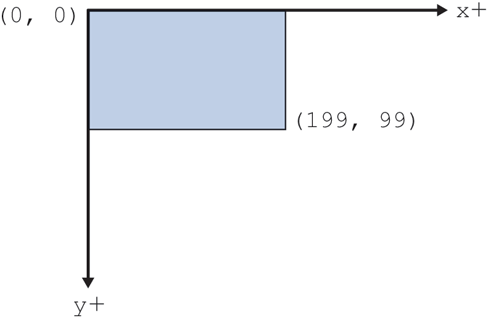
\includegraphics[width=\maxwidth,height=\maxheight,width=0.9\linewidth]{Figures/img_p136_1.png}
\end{center}

Điều này ban đầu có thể gây nhầm lẫn, vì bạn có thể đã quen với các hệ
tọa độ trong đó các giá trị \(y\) giảm dần khi bạn di chuyển xuống dưới.
Tuy nhiên, bạn sẽ sớm quen với nó thôi.

\subsection{Vẽ các đường và hình dạng (Drawing Lines and
Shapes)}\label{vux1ebd-cuxe1c-ux111ux1b0ux1eddng-vuxe0-huxecnh-dux1ea1ng-drawing-lines-and-shapes}

Vậy làm thế nào để bạn thực sự vẽ một cái gì đó? Để vẽ các hình dạng và
các đường thẳng, bạn không nói chuyện trực tiếp với
\texttt{DrawingPanel}, mà nói với một đối tượng liên quan có kiểu
\texttt{Graphics}. Hãy coi \texttt{DrawingPanel} như một bức tranh
canvas và đối tượng \texttt{Graphics} như một cây cọ vẽ. Lớp
\texttt{DrawingPanel} có một phương thức được gọi là
\texttt{getGraphics} để trả về đối tượng \texttt{Graphics} của nó:

\begin{verbatim}
Graphics g = panel.getGraphics();
\end{verbatim}

Một trong những lệnh vẽ đơn giản nhất là \texttt{drawLine}, nhận bốn đối
số số nguyên. Ví dụ, lời gọi phương thức:

\begin{verbatim}
g.drawLine(x1, y1, x2, y2);
\end{verbatim}

vẽ một đường thẳng từ điểm \((x_1, y_1)\) đến điểm \((x_2, y_2)\).
Phương thức \texttt{drawLine} chỉ là một trong nhiều lệnh mà một đối
tượng \texttt{Graphics} hiểu được; xem Bảng 3G.2 cho các lệnh khác. Đối
tượng \texttt{Graphics} có nhiều phương thức hơn ngoài các phương thức
được thảo luận ở đây. Bạn có thể đọc về chúng trong tài liệu Java API.

Bảng 3G.2 Một số phương thức hữu ích của đối tượng \texttt{Graphics}

\begin{center}

\includegraphics[width=\maxwidth,height=\maxheight,width=0.9\linewidth]{Figures/img_p138_0.png}
\end{center}

Dưới đây là một chương trình mẫu kết hợp những mảnh ghép này lại với
nhau:

\begin{verbatim}
 1  // Draws a line onto a DrawingPanel.
 2
 3  import java.awt.*;   // for graphics
 4
 5  public class DrawLine1 {
 6      public static void main(String[] args) {
 7          // create the drawing panel
 8          DrawingPanel panel = new DrawingPanel(200, 100);
 9
10          // draw a line on the panel using
11          // the Graphics paintbrush
12          Graphics g = panel.getGraphics();
13          g.drawLine(25, 75, 175, 25);
14      }
15  }
\end{verbatim}

Khi bạn chạy chương trình này, cửa sổ được hiển thị trong Hình 3G.2 sẽ
xuất hiện. Mặc dù nó không phải là văn bản trên giao diện điều khiển như
ở các chương trước, chúng sửa vẫn sẽ gọi đây là ``đầu ra'' của chương
trình.

Hình 3G.2 Đầu ra của \texttt{DrawLine1}

\begin{center}
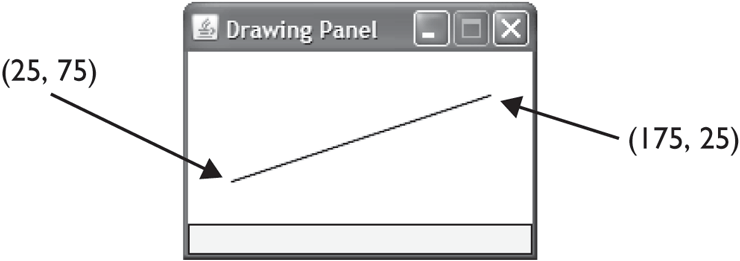
\includegraphics[width=\maxwidth,height=\maxheight,width=0.9\linewidth]{Figures/img_p139_0.png}
\end{center}

(Java có thể được chạy trên nhiều hệ thống khác nhau. Tùy thuộc vào hệ
điều hành của bạn, đầu ra của bạn có thể hơi khác so với các ảnh chụp
màn hình trong chương này.)

Câu lệnh đầu tiên trong \texttt{main} khởi tạo một \texttt{DrawingPanel}
với chiều rộng là 200 và chiều cao là 100. Khi nó đã được khởi tạo, cửa
sổ sẽ bật lên trên màn hình. Câu lệnh thứ hai vẽ một đường thẳng từ
\texttt{(25,\ 75)} đến \texttt{(175,\ 25)}. Điểm đầu tiên nằm ở phần
dưới bên trái của cửa sổ (25 điểm dịch từ bên trái, 75 điểm dịch từ trên
xuống). Điểm thứ hai nằm ở góc trên bên phải (175 điểm dịch từ bên trái,
25 điểm dịch từ trên xuống).

Hãy chú ý đến các dòng mã cụ thể này:

\begin{verbatim}
Graphics g = panel.getGraphics();
g.drawLine(25, 75, 175, 25);
\end{verbatim}

Bạn có thể tự hỏi tại sao bạn không thể nói đơn giản là:

\begin{verbatim}
panel.drawLine(25, 75, 175, 25);   // this is illegal
\end{verbatim}

Vấn đề là có hai đối tượng khác nhau tham gia vào chương trình này: bản
thân \texttt{DrawingPanel} (bức tranh canvas) và đối tượng
\texttt{Graphics} liên kết với panel (cây cọ vẽ). Panel không biết cách
vẽ một đường thẳng; chỉ có đối tượng \texttt{Graphics} mới biết cách
thực hiện việc này. Bạn phải cẩn thận để đảm bảo rằng bạn đang nói
chuyện với đúng đối tượng khi bạn đưa ra một lệnh.

Yêu cầu này có thể gây nhầm lẫn, nhưng nó rất phổ biến trong các chương
trình Java. Trên thực tế, trong một chương trình Java điển hình, có hàng
trăm (nếu không muốn nói là hàng nghìn) đối tượng tương tác với nhau.
Những tương tác này không khác nhiều so với tương tác giữa con người với
nhau. Nếu bạn muốn lên lịch một cuộc họp, một giám đốc điều hành bận rộn
của công ty có thể nói với bạn, ``Hãy nói chuyện với thư ký của tôi về
điều đó.'' Hoặc nếu bạn đang hỏi những câu hỏi pháp lý khó, một người có
thể nói với bạn, ``Hãy nói chuyện với luật sư của tôi về điều đó.''
Trong trường hợp này, \texttt{DrawingPanel} không biết cách vẽ, vì vậy
nếu nó có thể nói, nó sẽ nói, ``Hãy nói chuyện với đối tượng
\texttt{Graphics} của tôi về điều đó.''

Sử dụng đối tượng \texttt{Graphics} mà không lưu trữ nó trong một biến
cũng hợp lệ, như thế này:

\begin{verbatim}
panel.getGraphics().drawLine(25, 75, 175, 25);    // also legal
\end{verbatim}

Nhưng bạn sẽ thường muốn gửi một số lệnh đến đối tượng
\texttt{Graphics}, vì vậy sẽ thuận tiện hơn khi đặt tên cho nó và lưu
trữ nó trong một biến.

Hãy xem một ví dụ phức tạp hơn:

\begin{verbatim}
 1  // Draws three lines to make a triangle.
 2
 3  import java.awt.*;
 4
 5  public class DrawLine2 {
 6      public static void main(String[] args) {
 7          DrawingPanel panel = new DrawingPanel(200, 100);
 8
 9          // draw a triangle on the panel
10          Graphics g = panel.getGraphics();
11          g.drawLine(25, 75, 100, 25);
12          g.drawLine(100, 25, 175, 75);
13          g.drawLine(25, 75, 175, 75);
14      }
15  }
\end{verbatim}

Chương trình này vẽ ba đường thẳng khác nhau để tạo thành một hình tam
giác, như được hiển thị trong Hình 3G.3. Các đường thẳng được vẽ giữa ba
điểm khác nhau. Ở góc dưới bên trái, chúng ta có điểm
\texttt{(25,\ 75)}. Ở giữa phía trên, chúng ta có điểm
\texttt{(100,\ 25)}. Và ở góc dưới bên phải, chúng ta có điểm
\texttt{(175,\ 75)}. Các lời gọi khác nhau trên \texttt{drawLine} chỉ
đơn giản là vẽ các đường thẳng nối ba điểm này lại.

Hình 3G.3 Đầu ra của \texttt{DrawLine2}

\begin{center}
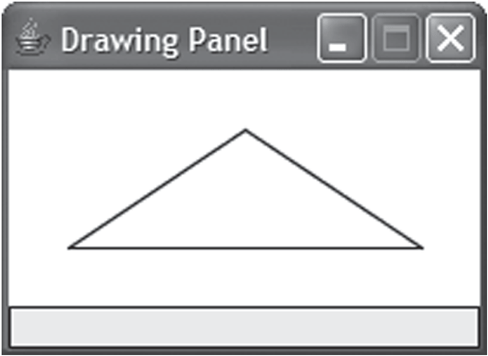
\includegraphics[width=\maxwidth,height=\maxheight,width=0.9\linewidth]{Figures/img_p142_0.png}
\end{center}

Đối tượng \texttt{Graphics} cũng có các phương thức để vẽ các hình dạng
cụ thể. Ví dụ, bạn có thể vẽ các hình chữ nhật với phương thức
\texttt{drawRect}:

\begin{verbatim}
g.drawRect(x, y, width, height);
\end{verbatim}

Câu lệnh này vẽ một hình chữ nhật có tọa độ góc trên bên trái là
\((x, y)\) và chiều cao cùng chiều rộng cho trước.

Một hình dạng khác mà bạn thường muốn vẽ là một hình tròn hoặc, tổng
quát hơn là một hình bầu dục (oval). Nhưng làm thế nào để bạn xác định
nó xuất hiện ở đâu và nó lớn đến mức nào?

Điều bạn thực sự chỉ định là cái được gọi là ``bounding rectangle''
(hình chữ nhật giới hạn) của hình tròn hoặc hình bầu dục. Java sẽ vẽ
hình bầu dục lớn nhất có thể nằm gọn bên trong hình chữ nhật đó. Vì vậy,
lời gọi phương thức:

\begin{verbatim}
g.drawOval(x, y, width, height);
\end{verbatim}

sẽ vẽ hình bầu dục lớn nhất vừa với hình chữ nhật có tọa độ góc trên bên
trái \((x, y)\) và chiều cao cùng chiều rộng cho trước.

Chú ý rằng hai giá trị đầu tiên được truyền vào \texttt{drawRect} và
\texttt{drawOval} là các tọa độ, trong khi hai giá trị tiếp theo là
chiều rộng và chiều cao. Ví dụ, đây là một chương trình ngắn vẽ hai hình
chữ nhật và hai hình bầu dục:

\begin{verbatim}
 1  // Draws several shapes.
 2
 3  import java.awt.*;
 4
 5  public class DrawShapes1 {
 6      public static void main(String[] args) {
 7          DrawingPanel panel = new DrawingPanel(200, 100);
 8
 9          Graphics g = panel.getGraphics();
10          g.drawRect(25, 50, 20, 20);
11          g.drawRect(150, 10, 40, 20);
12          g.drawOval(50, 25, 20, 20);
13          g.drawOval(150, 50, 40, 20);
14      }
15  }
\end{verbatim}

Hình 3G.4 cho thấy đầu ra của chương trình.

Hình 3G.4 Đầu ra của \texttt{DrawShapes1}

\begin{center}

\includegraphics[width=\maxwidth,height=\maxheight,width=0.9\linewidth]{Figures/img_p144_0.png}
\end{center}

Hình chữ nhật đầu tiên có góc trên bên trái của nó ở tọa độ
\texttt{(25,\ 50)}. Chiều rộng và chiều cao của nó đều là 20, vì vậy đây
là một hình vuông. Tọa độ của góc dưới bên phải của nó sẽ là
\texttt{(45,\ 70)}, hay lớn hơn tọa độ \((x, y)\) của góc trên bên trái
20 đơn vị. Chương trình cũng vẽ một hình chữ nhật có góc trên bên trái
tại \texttt{(150,\ 10)} có chiều rộng là 40 và chiều cao là 20 (rộng hơn
cao). Hình chữ nhật giới hạn của hình bầu dục đầu tiên có tọa độ góc
trên bên trái là \texttt{(50,\ 25)} và chiều rộng cũng như chiều cao là
20. Nói cách khác, nó là một hình tròn.

Hình chữ nhật giới hạn của hình bầu dục thứ hai có tọa độ góc trên bên
trái là \texttt{(150,\ 50)}, chiều rộng là 40, và chiều cao là 20 (nó là
một hình bầu dục rộng hơn là cao).

Đôi khi bạn không chỉ muốn vẽ đường viền (outline) của một hình dạng;
bạn muốn tô màu (paint) toàn bộ khu vực bằng một màu cụ thể. Có các biến
thể của các phương thức \texttt{drawRect} và \texttt{drawOval} được gọi
là \texttt{fillRect} và \texttt{fillOval} thực hiện chính xác điều đó,
vẽ một hình chữ nhật hoặc hình bầu dục và tô màu nó bằng màu sơn hiện
tại (mặc định là màu đen). Hãy thay đổi hai trong số các lời gọi trong
chương trình trước thành các thao tác ``tô màu'' (fill) thay vì các thao
tác ``vẽ'' (draw):

\begin{verbatim}
 1  // Draws and fills several shapes.
 2
 3  import java.awt.*;
 4
 5  public class DrawShapes2 {
 6      public static void main(String[] args) {
 7          DrawingPanel panel = new DrawingPanel(200, 100);
 8
 9          Graphics g = panel.getGraphics();
10          g.fillRect(25, 50, 20, 20);
11          g.drawRect(150, 10, 40, 20);
12          g.drawOval(50, 25, 20, 20);
13          g.fillOval(150, 50, 40, 20);
14      }
15  }
\end{verbatim}

Bây giờ chúng ta sẽ nhận được đầu ra được hiển thị trong Hình 3G.5 thay
thế.

Hình 3G.5 Đầu ra của \texttt{DrawShapes2}

\begin{center}
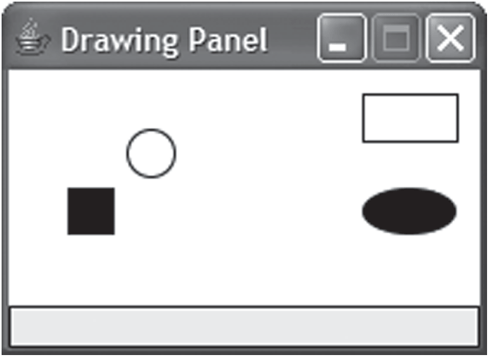
\includegraphics[width=\maxwidth,height=\maxheight,width=0.9\linewidth]{Figures/img_p146_1.png}
\end{center}

\subsection{Màu sắc (Colors)}\label{muxe0u-sux1eafc-colors}

Tất cả các hình dạng và đường thẳng được vẽ bởi các chương trình trước
đều có màu đen, và tất cả các panel đều có nền màu trắng. Đây là các màu
mặc định, nhưng bạn có thể thay đổi màu nền của panel, và bạn có thể
thay đổi màu được sử dụng bởi đối tượng \texttt{Graphics} bao nhiêu lần
tùy thích. Để thay đổi các màu này, bạn sử dụng lớp \texttt{Color} tiêu
chuẩn, là một phần của gói \texttt{java.awt}.

Có một số màu được định nghĩa sẵn mà bạn có thể tham chiếu trực tiếp.
Chúng được định nghĩa dưới dạng các hằng số lớp (class constants) trong
lớp \texttt{Color} (giống như nhiều hằng số chúng ta đã sử dụng trong
Chương 2). Tên của các hằng số này đều được viết hoa và mang tính tự
giải thích. Để tham chiếu đến một trong những màu này, bạn phải đặt
trước nó bằng tên lớp và dấu chấm, như \texttt{Color.GREEN} hoặc
\texttt{Color.BLUE}. Các hằng số \texttt{Color} được định nghĩa sẵn được
liệt kê trong Bảng 3G.3.

Bảng 3G.3 Các hằng số Màu (Color Constants)

\begin{center}

\includegraphics[width=\maxwidth,height=\maxheight,width=0.9\linewidth]{Figures/img_p147_0.png}
\end{center}

Như đã đề cập trước đó, đối tượng \texttt{DrawingPanel} có một phương
thức có thể được sử dụng để thay đổi màu nền bao phủ toàn bộ panel:

\begin{verbatim}
panel.setBackground(Color.YELLOW);
\end{verbatim}

Tương tự, đối tượng \texttt{Graphics} có một phương thức có thể được sử
dụng để thay đổi màu hiện tại dùng để vẽ hoặc tô màu các hình dạng và
đường thẳng:

\begin{verbatim}
g.setColor(Color.MAGENTA);
\end{verbatim}

Việc gọi \texttt{setColor} giống như nhúng cây cọ vẽ của bạn vào một màu
sơn khác. Từ thời điểm đó trở đi, tất cả các thao tác vẽ và tô màu sẽ
được thực hiện bằng màu đã chỉ định. Ví dụ, dưới đây là một phiên bản
khác của chương trình trước đó sử dụng màu nền lục lam (cyan - xanh
nhạt) và tô màu hình bầu dục và hình vuông bằng màu trắng thay vì màu
đen:

\begin{verbatim}
 1  // Draws and fills shapes in different colors.
 2
 3  import java.awt.*;
 4
 5  public class DrawColoredShapes {
 6      public static void main(String[] args) {
 7          DrawingPanel panel = new DrawingPanel(200, 100);
 8          panel.setBackground(Color.CYAN);
 9
10          Graphics g = panel.getGraphics();
11          g.drawRect(150, 10, 40, 20);
12          g.drawOval(50, 25, 20, 20);
13          g.setColor(Color.WHITE);
14          g.fillOval(150, 50, 40, 20);
15          g.fillRect(25, 50, 20, 20);
16      }
17  }
\end{verbatim}

Chương trình này tạo ra đầu ra được hiển thị trong Hình 3G.6. (Các hình
ảnh được hiển thị trong cuốn sách giáo khoa này có thể không khớp với
các màu bạn sẽ thấy trên màn hình của mình.)

Hình 3G.6 Đầu ra của \texttt{DrawColoredShapes}

\begin{center}

\includegraphics[width=\maxwidth,height=\maxheight,width=0.9\linewidth]{Figures/img_p148_0.png}
\end{center}

Lưu ý rằng bạn yêu cầu panel thiết lập màu nền (background color), trong
khi bạn yêu cầu đối tượng \texttt{Graphics} thiết lập màu tiền cảnh
(foreground color). Lý do là màu nền là một thuộc tính của toàn bộ cửa
sổ, trong khi màu tiền cảnh chỉ ảnh hưởng đến các hình dạng cụ thể mà
bạn vẽ.

Lưu ý thêm rằng thứ tự của các lời gọi đã được sắp xếp lại. Hai lệnh vẽ
xuất hiện trước, sau đó là lời gọi trên \texttt{setColor} để thay đổi
màu thành màu trắng, rồi đến hai lệnh tô màu. Điều này đảm bảo rằng thao
tác vẽ được thực hiện bằng màu đen và thao tác tô màu được thực hiện
bằng màu trắng. Thứ tự các phép toán rất quan trọng trong các chương
trình vẽ này, do đó bạn sẽ phải theo dõi xem màu hiện tại của mình là gì
mỗi khi bạn đưa ra lệnh mới để vẽ hoặc tô màu một cái gì đó.

\begin{center}
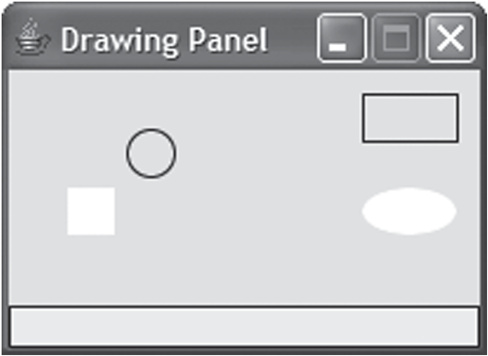
\includegraphics[width=\maxwidth,height=\maxheight,width=0.9\linewidth]{Figures/img_p149_0.png}
\end{center}

\begin{quote}
{[}!WARNING{]} LỖI LẬP TRÌNH PHỔ BIẾN \textbf{Hiểu lầm về Draw so với
Fill}

Một số lập trình viên mới nghĩ rằng một hình dạng phải được vẽ (chẳng
hạn như với \texttt{drawRect}) trước khi nó có thể được tô màu (chẳng
hạn như với \texttt{fillRect}). Điều này không đúng. Trên thực tế, khi
bạn đang cố gắng vẽ một hình dạng có đường viền (outlined shape), đây
chính xác là điều sai lầm. Giả sử bạn muốn vẽ một hình chữ nhật màu xanh
lá cây kích thước \(60 \times 30\) với viền đen tại tọa độ
\texttt{(20,\ 50)}. Bạn có thể viết mã sau:

\begin{verbatim}
g.setColor(Color.BLACK);   // incorrect code
g.drawRect(20, 50, 60, 30);
g.setColor(Color.GREEN);
g.fillRect(20, 50, 60, 30);
\end{verbatim}

Tuy nhiên, lệnh \texttt{fill} bao phủ các pixel giống hệt như lệnh
\texttt{draw}, và phần bên trong màu xanh lá cây sẽ được vẽ đè lên đường
viền màu đen, dẫn đến diện mạo sau:

\begin{center}
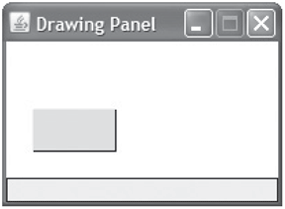
\includegraphics[width=\maxwidth,height=\maxheight,width=0.9\linewidth]{Figures/img_p151_0.png}
\end{center}

Thay vào đó, mã nên tô màu phần bên trong của hình chữ nhật trước, sau
đó mới vẽ đường viền màu đen, để đảm bảo rằng đường viền hiển thị nằm
trên phần tô màu. Dưới đây là đoạn mã chính xác và đầu ra của nó:

\begin{verbatim}
g.setColor(Color.GREEN);   // corrected code
g.fillRect(20, 50, 60, 30);
g.setColor(Color.BLACK);
g.drawRect(20, 50, 60, 30);
\end{verbatim}

\begin{center}
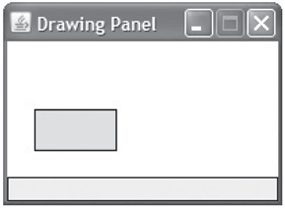
\includegraphics[width=\maxwidth,height=\maxheight,width=0.9\linewidth]{Figures/img_p151_1.png}
\end{center}
\end{quote}

\subsection{Vẽ bằng các vòng lặp (Drawing with
Loops)}\label{vux1ebd-bux1eb1ng-cuxe1c-vuxf2ng-lux1eb7p-drawing-with-loops}

Trong mỗi ví dụ trước, chúng ta đã sử dụng các hằng số đơn giản cho các
lệnh vẽ và tô màu, nhưng có thể sử dụng các biểu thức (expressions). Ví
dụ, giả sử chúng ta bám sát kích thước \texttt{DrawingPanel} của mình là
rộng 200 pixel và cao 100 pixel và chúng ta muốn tạo ra một chuỗi bốn
hình chữ nhật nằm chéo kéo dài từ góc trên bên trái đến góc dưới bên
phải, mỗi hình chứa một hình bầu dục màu trắng bên trong. Nói cách khác,
chúng ta muốn tạo ra đầu ra được hiển thị trong Hình 3G.7.

Hình 3G.7 Đầu ra mong muốn của \texttt{DrawLoop1}

\begin{center}
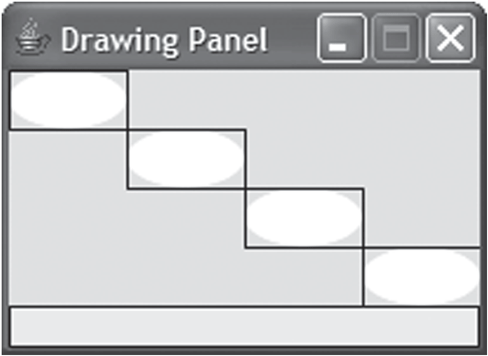
\includegraphics[width=\maxwidth,height=\maxheight,width=0.9\linewidth]{Figures/img_p152_1.png}
\end{center}

Chiều rộng tổng thể 200 và chiều cao tổng thể 100 được chia đều thành
bốn hình chữ nhật, có nghĩa là tất cả chúng đều phải rộng 50 pixel và
cao 25 pixel. Vì vậy, giá trị chiều rộng và chiều cao cho cả bốn hình
chữ nhật là giống nhau, nhưng vị trí góc trên bên trái của chúng thì
khác nhau. Góc trên bên trái của hình chữ nhật đầu tiên là ở
\texttt{(0,\ 0)}, cái thứ hai là ở \texttt{(50,\ 25)}, cái thứ ba là ở
\texttt{(100,\ 50)} và cái thứ tư là ở \texttt{(150,\ 75)}. Chúng ta cần
viết mã để tạo ra các tọa độ khác nhau này.

\begin{center}

\includegraphics[width=\maxwidth,height=\maxheight,width=0.9\linewidth]{Figures/img_p153_0.png}
\end{center}

Đây là một nơi tuyệt vời để sử dụng vòng lặp \texttt{for}. Sử dụng các
kỹ thuật được giới thiệu trong Chương 2, chúng ta có thể lập một bảng và
phát triển một công thức cho các tọa độ. Trong trường hợp này, sẽ dễ
dàng hơn nếu vòng lặp bắt đầu bằng \texttt{0} thay vì \texttt{1}, điều
này thường xảy ra với các chương trình vẽ. Dưới đây là một chương trình
tạo ra nỗ lực đầu tiên tốt để tạo ra đầu ra mong muốn:

\begin{verbatim}
 1  // Draws boxed ovals using a for loop (flawed version).
 2
 3  import java.awt.*;
 4
 5  public class DrawLoop1 {
 6      public static void main(String[] args) {
 7          DrawingPanel panel = new DrawingPanel(200, 100);
 8          panel.setBackground(Color.CYAN);
 9
10          Graphics g = panel.getGraphics();
11          for (int i = 0; i < 4; i++) {
12              g.drawRect(i * 50, i * 25, 50, 25);
13              g.setColor(Color.WHITE);
14              g.fillOval(i * 50, i * 25, 50, 25);
15          }
16      }
17  }
\end{verbatim}

Chương trình này tạo ra đầu ra được hiển thị trong Hình 3G.8.

Hình 3G.8 Đầu ra của \texttt{DrawLoop1}

\begin{center}
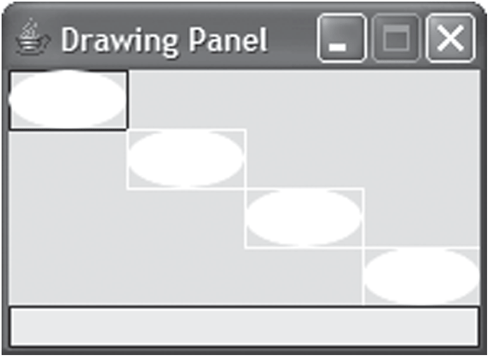
\includegraphics[width=\maxwidth,height=\maxheight,width=0.9\linewidth]{Figures/img_p154_1.png}
\end{center}

Tọa độ và kích thước đã đúng, nhưng màu sắc thì không. Thay vì có được
bốn hình chữ nhật màu đen có hình bầu dục màu trắng bên trong, chúng ta
lại có một hình chữ nhật màu đen và ba hình chữ nhật màu trắng. Đó là vì
chúng ta chỉ có một lời gọi \texttt{setColor} bên trong vòng lặp. Ban
đầu màu sắc sẽ

được đặt thành màu đen, đó là lý do tại sao hình chữ nhật đầu tiên xuất
hiện màu đen. Nhưng khi chúng ta gọi \texttt{setColor} thay đổi màu
thành màu trắng, mọi lệnh vẽ và tô màu tiếp theo đều được thực hiện bằng
màu trắng, bao gồm cả hình chữ nhật thứ hai, thứ ba và thứ tư.

Vì vậy, chúng ta cần bao gồm các lời gọi để đặt màu thành màu đen, để vẽ
các hình chữ nhật và đặt màu thành màu trắng để vẽ các hình bầu dục được
tô màu. Đồng thời, tốt nhất là nên đổi thứ tự các tác vụ này. Các hình
chữ nhật và hình bầu dục chồng lên nhau một chút, và chúng ta muốn hình
chữ nhật được vẽ đè lên hình bầu dục hơn là ngược lại. Chương trình sau
đây tạo ra đầu ra chính xác:

\begin{verbatim}
 1  // Draws boxed ovals using a for loop.
 2
 3  import java.awt.*;
 4
 5  public class DrawLoop2 {
 6      public static void main(String[] args) {
 7          DrawingPanel panel = new DrawingPanel(200, 100);
 8          panel.setBackground(Color.CYAN);
 9
10          Graphics g = panel.getGraphics();
11          for (int i = 0; i < 4; i++) {
12              g.setColor(Color.WHITE);
13              g.fillOval(i * 50, i * 25, 50, 25);
14              g.setColor(Color.BLACK);
15              g.drawRect(i * 50, i * 25, 50, 25);
16          }
17      }
18  }
\end{verbatim}

Cũng có thể tự tạo các đối tượng \texttt{Color} tùy chỉnh, thay vì sử
dụng các màu hằng số được cung cấp trong lớp \texttt{Color}. Màn hình
máy tính sử dụng đỏ, xanh lá cây và xanh dương (RGB) làm các màu cơ bản,
vì vậy khi bạn khởi tạo một đối tượng \texttt{Color}, bạn sẽ truyền các
giá trị tham số của riêng mình cho độ đỏ (redness), độ xanh lá cây
(greenness) và độ xanh dương (blueness) của màu sắc:

\begin{verbatim}
new Color(red, green, blue)
\end{verbatim}

Các thành phần đỏ/xanh lá cây/xanh dương phải là các giá trị số nguyên
từ \texttt{0} đến \texttt{255}. Giá trị càng cao, thì càng có nhiều màu
đó được trộn vào. Tất cả giá trị \texttt{0} tạo ra màu đen, và tất cả
giá trị \texttt{255} tạo ra màu trắng. Các giá trị
\texttt{(0,\ 255,\ 0)} tạo ra một màu xanh lá cây thuần túy, trong khi
các giá trị \texttt{(128,\ 0,\ 128)} tạo ra một màu tím đậm (bởi vì màu
đỏ và màu xanh dương được pha trộn). Hãy tìm kiếm ``RGB table'' trên
công cụ tìm kiếm yêu thích của bạn để tìm bảng các màu thông dụng.

Chương trình sau minh họa việc sử dụng các màu tùy chỉnh. Nó sử dụng một
hằng số lớp cho số lượng hình chữ nhật để vẽ và tạo ra một sự pha trộn
(blend) màu sắc từ đen sang trắng:

\begin{verbatim}
 1  // Draws a smooth color gradient from black to white.
 2
 3  import java.awt.*;
 4
 5  public class DrawColorGradient {
 6      public static final int RECTS = 32;
 7
 8      public static void main(String[] args) {
 9          DrawingPanel panel = new DrawingPanel(256, 256);
10          panel.setBackground(new Color(255, 128, 0)); // orange
11
12          Graphics g = panel.getGraphics();
13
14          // from black to white, top left to bottom right
15          for (int i = 0; i < RECTS; i++) {
16              int shift = i * 256 / RECTS;
17              g.setColor(new Color(shift, shift, shift));
18              g.fillRect(shift, shift, 20, 20);
19          }
20      }
21  }
\end{verbatim}

Chương trình này tạo ra đầu ra được hiển thị trong Hình 3G.9.

Hình 3G.9 Đầu ra của \texttt{DrawColorGradient}

\begin{center}

\includegraphics[width=\maxwidth,height=\maxheight,width=0.9\linewidth]{Figures/img_p157_0.png}
\end{center}

Lưu trữ một đối tượng \texttt{Color} vào một biến hoặc truyền nó như một
tham số cũng là hợp lệ. Ví dụ, chúng ta có thể viết mã tô màu trong
chương trình trước như sau:

\begin{verbatim}
Color c = new Color(shift, shift, shift);
g.setColor(c);
...
\end{verbatim}

\begin{center}
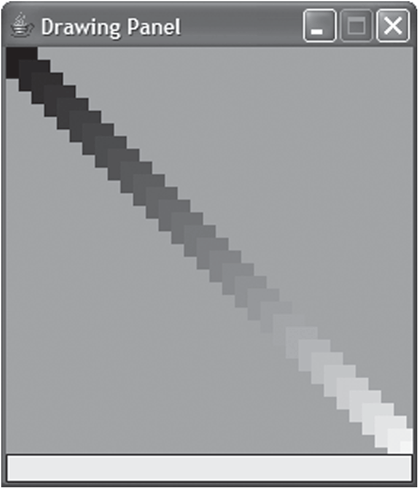
\includegraphics[width=\maxwidth,height=\maxheight,width=0.9\linewidth]{Figures/img_p158_0.png}
\end{center}

Chúng ta sẽ sử dụng ý tưởng này sau khi tham số hóa (parameterizing) màu
sắc trong Nghiên cứu điển hình (Case Study) của chương này.

\subsection{Văn bản và Phông chữ (Text and
Fonts)}\label{vux103n-bux1ea3n-vuxe0-phuxf4ng-chux1eef-text-and-fonts}

Một lệnh vẽ khác đáng được nhắc đến có thể được sử dụng để đưa văn bản
vào các bức vẽ của bạn. Phương thức \texttt{drawString} của đối tượng
\texttt{Graphics} sẽ vẽ một đối tượng \texttt{String} được cung cấp với
góc dưới bên trái của nó ở tọa độ \((x, y)\):

\begin{verbatim}
g.drawString(message, x, y);
\end{verbatim}

Quy ước này hơi khác một chút so với quy ước chúng ta đã sử dụng cho
\texttt{drawRect}. Với \texttt{drawRect}, chúng ta đã chỉ định các tọa
độ của góc trên bên trái. Ở đây, chúng ta chỉ định các tọa độ của góc
dưới bên trái. Theo mặc định, văn bản được vẽ với chiều cao xấp xỉ 10
pixel. Dưới đây là một chương trình mẫu sử dụng một vòng lặp để vẽ một
đối tượng \texttt{String} cụ thể 10 lần khác nhau, mỗi lần thụt lề 5
pixel sang bên phải và di chuyển xuống 10 pixel từ trên cùng:

\begin{verbatim}
 1  // Draws a message several times.
 2
 3  import java.awt.*;
 4
\end{verbatim}

\begin{verbatim}
 5  public class DrawStringMessage1 {
 6      public static void main(String[] args) {
 7          DrawingPanel panel = new DrawingPanel(200, 100);
 8          panel.setBackground(Color.YELLOW);
 9
10          Graphics g = panel.getGraphics();
11          for (int i = 0; i < 10; i++) {
12              g.drawString("There is no place like home",
13                          i * 5, 10 + i * 10);
14          }
15      }
16  }
\end{verbatim}

Chương trình này tạo ra đầu ra được hiển thị trong Hình 3G.10.

Hình 3G.10 Đầu ra của \texttt{DrawStringMessage}

\begin{center}
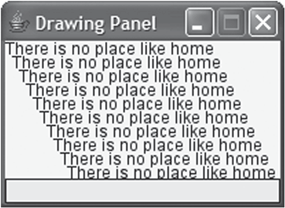
\includegraphics[width=\maxwidth,height=\maxheight,width=0.9\linewidth]{Figures/img_p160_1.png}
\end{center}

Phông chữ (fonts) được sử dụng để mô tả các kiểu dáng (styles) khác nhau
để viết các ký tự trên màn hình. Nếu bạn muốn thay đổi kiểu hoặc kích
thước của văn bản trên màn hình, bạn có thể sử dụng phương thức
\texttt{setFont} của đối tượng \texttt{Graphics}.

\textbf{Phông chữ (Font)} Một thiết kế tổng thể cho một tập hợp các ký
tự văn bản, bao gồm kiểu, kích thước, độ đậm (weight) và diện mạo của
từng ký tự.

Phương thức này thay đổi kích thước và kiểu văn bản mà các chuỗi được
vẽ.

Tham số truyền vào \texttt{setFont} là một đối tượng \texttt{Font}. Một
đối tượng \texttt{Font} được tạo ra bằng cách truyền vào ba tham
số---tên của phông chữ dưới dạng \texttt{String}, kiểu của nó (chẳng hạn
như in đậm hoặc in nghiêng), và kích thước của nó dưới dạng số nguyên:

\begin{verbatim}
new Font(name, style, size)
\end{verbatim}

Các kiểu phông chữ phổ biến như in đậm (bold) được triển khai dưới dạng
các hằng số trong lớp \texttt{Font}. Các hằng số có sẵn và một số tên
phông chữ phổ biến được liệt kê trong các Bảng 3G.4 và 3G.5.

Bảng 3G.4 Các hằng số hữu ích của lớp \texttt{Font}

\begin{center}

\includegraphics[width=\maxwidth,height=\maxheight,width=0.9\linewidth]{Figures/img_p161_0.png}
\end{center}

Bảng 3G.5 Các Tên Phông Chữ Phổ Biến

\begin{center}

\includegraphics[width=\maxwidth,height=\maxheight,width=0.9\linewidth]{Figures/img_p162_0.png}
\end{center}

Giống như trường hợp của màu sắc, việc thiết lập phông chữ chỉ ảnh hưởng
đến các chuỗi được vẽ sau khi phông chữ được thiết lập. Chương trình sau
đây thiết lập một số phông chữ và sử dụng chúng để vẽ các chuỗi:

\begin{verbatim}
 1  // Draws several messages using different fonts.
 2
 3  import java.awt.*;
 4
 5  public class DrawFonts {
 6      public static void main(String[] args) {
 7          DrawingPanel panel = new DrawingPanel(200, 100);
 8          panel.setBackground(Color.PINK);
 9
10          Graphics g = panel.getGraphics();
11          g.setFont(new Font("Monospaced",
12                     Font.BOLD + Font.ITALIC, 36));
13          g.drawString("Too big", 20, 40);
14
15          g.setFont(new Font("SansSerif", Font.PLAIN, 10));
16          g.drawString("Too small", 30, 60);
17
18          g.setFont(new Font("Serif", Font.ITALIC, 18));
19          g.drawString("Just right", 40, 80);
20      }
21  }
\end{verbatim}

Chương trình này tạo ra đầu ra được hiển thị trong Hình 3G.11.

Hình 3G.11 Đầu ra của \texttt{DrawFonts}

\begin{center}
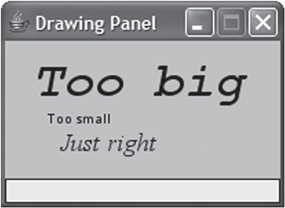
\includegraphics[width=\maxwidth,height=\maxheight,width=0.9\linewidth]{Figures/img_p163_0.png}
\end{center}

\subsection{Hình ảnh (Images)}\label{huxecnh-ux1ea3nh-images}

\texttt{DrawingPanel} cũng có khả năng hiển thị các hình ảnh được tải từ
các tệp ở các định dạng như JPEG, PNG và GIF. Để hiển thị một hình ảnh,
đầu tiên bạn phải tìm một tệp hình ảnh (chẳng hạn như một tệp trên
internet hoặc trên máy tính của bạn) và đặt nó vào cùng thư mục với dự
án mã của bạn. Hình ảnh được hiển thị qua hai bước: đầu tiên, hình ảnh
phải được tải từ ổ cứng vào một đối tượng \texttt{Image}, và sau đó đối
tượng \texttt{Graphics} của panel có thể hiển thị hình ảnh.

\begin{verbatim}
Image img = panel.loadImage("smileyface.png");
g.drawImage(img, x, y, panel);
\end{verbatim}

Các tọa độ \(x\) và \(y\) được truyền vào khi vẽ hình ảnh thể hiện vị
trí pixel ở góc trên cùng/bên trái của nó.

Có một vài điều kỳ quặc đối với cú pháp. Một là chúng ta sử dụng
\texttt{DrawingPanel} để tải hình ảnh, trong khi bạn sử dụng đối tượng
\texttt{Graphics} để vẽ nó. Rất dễ vô tình lẫn lộn hai thứ này. Ngoài
ra, không giống như các lệnh vẽ khác, \texttt{drawImage} yêu cầu bạn
truyền \texttt{DrawingPanel} làm tham số cuối cùng cho phương thức. Điều
này được yêu cầu bởi lớp \texttt{Graphics} của Java để mã có thể biên
dịch.

Ví dụ, chương trình sau đây tải một hình ảnh trông giống như bức vẽ của
một cầu vồng và vẽ nó lên \texttt{DrawingPanel} với một chuỗi văn bản
nằm dưới nó.

\begin{verbatim}
 1  // This program displays a rainbow from an image file.
 2  import java.awt.*;
 3
 4  public class DrawRainbow {
 5      public static void main(String[] args) {
 6          DrawingPanel panel = new DrawingPanel(280, 200);
 7          Image rainbow = panel.loadImage("rainbow.png");
 8          Graphics g = panel.getGraphics();
 9          g.drawImage(rainbow, 0, 0, panel);
10          g.drawString("Somewhere over the rainbow...", 10, 
11 180);
12      }
13  }
\end{verbatim}

Chương trình tạo ra đầu ra được hiển thị trong Hình 3G.12.

\begin{center}

\includegraphics[width=\maxwidth,height=\maxheight,width=0.9\linewidth]{Figures/img_p164_0.png}
\end{center}

Hình 3G.12 Đầu ra của \texttt{DrawRainbow}

Nếu bạn muốn vẽ cùng một hình ảnh nhiều lần trên panel, bạn không cần
phải lặp lại phần \texttt{loadImage} của quá trình này. Việc tải hình
ảnh một lần duy nhất và sau đó vẽ nó bao nhiêu lần tùy thích sẽ hiệu quả
hơn nhiều. Đoạn mã sau đây sẽ vẽ một vài bản sao của một hình ảnh trong
một tệp có tên là \texttt{smiley.png}, có kích thước \(100 \times 100\)
pixel. Đầu ra của đoạn mã này được hiển thị trong Hình 3G.13.

Hình 3G.13 Đầu ra mặt cười

\begin{center}
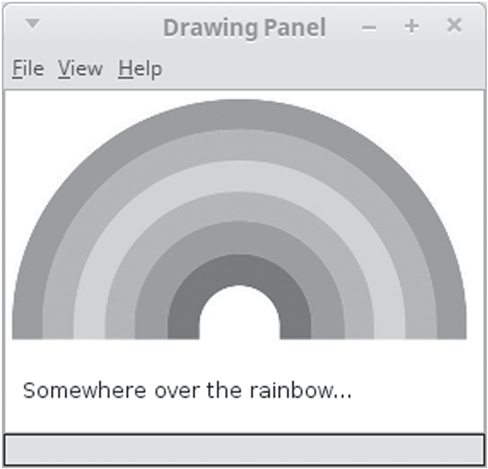
\includegraphics[width=\maxwidth,height=\maxheight,width=0.9\linewidth]{Figures/img_p165_1.png}
\end{center}

\begin{verbatim}
Image smileyFace = panel.loadImage("smiley.png");
Graphics g = panel.getGraphics();
for (int i = 0; i < 4; i++) {
    g.drawImage(smileyFace, i * 110 + 10, 10, panel);
}
\end{verbatim}

\begin{center}
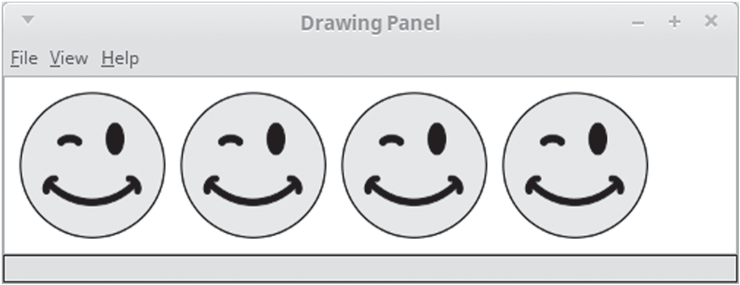
\includegraphics[width=\maxwidth,height=\maxheight,width=0.9\linewidth]{Figures/img_p166_0.png}
\end{center}

\subsection{3G.2 Phân rã thủ tục với Đồ họa (Procedural Decomposition
with
Graphics)}\label{g.2-phuxe2n-ruxe3-thux1ee7-tux1ee5c-vux1edbi-ux111ux1ed3-hux1ecda-procedural-decomposition-with-graphics-1}

Nếu bạn viết các chương trình vẽ phức tạp, bạn sẽ muốn chia nhỏ chúng
thành một số phương thức tĩnh (static methods) để cấu trúc mã và loại bỏ
sự dư thừa. Khi thực hiện việc này, bạn sẽ phải truyền đối tượng
\texttt{Graphics} cho từng phương thức tĩnh mà bạn giới thiệu. Để lấy
một ví dụ nhanh, chương trình \texttt{DrawStringMessage1} từ phần trước
có thể được chia thành một phương thức \texttt{main} và một phương thức
\texttt{drawText}, như sau:

\begin{verbatim}
 1  // Draws a message several times using a static method.
 2
 3  import java.awt.*;
 4
 5  public class DrawStringMessage2 {
 6      public static void main(String[] args) {
 7          DrawingPanel panel = new DrawingPanel(200, 100);
 8          panel.setBackground(Color.YELLOW);
 9
10          Graphics g = panel.getGraphics();
11          drawText(g);
12      }
13
14      public static void drawText(Graphics g) {
15          for (int i = 0; i < 10; i++) {
16              g.drawString("There is no place like home",
17                           i * 5, 10 + i * 10);
18          }
19      }
20  }
\end{verbatim}

Chương trình này tạo ra cùng một đầu ra như chương trình gốc (Hình
3G.10).

Chương trình sẽ không biên dịch được nếu không truyền
\texttt{Graphics\ g} cho phương thức \texttt{drawText}, bởi vì
\texttt{g} là cần thiết để gọi các phương thức vẽ như
\texttt{drawString} và \texttt{fillRect}.

\subsubsection{Một ví dụ lớn hơn: DrawDiamonds (A Larger Example:
DrawDiamonds)}\label{mux1ed9t-vuxed-dux1ee5-lux1edbn-hux1a1n-drawdiamonds-a-larger-example-drawdiamonds}

Bây giờ chúng ta hãy xem xét một tác vụ phức tạp hơn một chút: vẽ hình
thoi (diamond) lớn nhất có thể nằm vừa trong một hộp có kích thước cụ
thể. Hình thoi lớn nhất có thể nằm vừa trong một hộp có kích thước
\(50 \times 50\) được hiển thị trong Hình 3G.14.

Hình 3G.14 Hình thoi (Diamond)

\begin{center}

\includegraphics[width=\maxwidth,height=\maxheight,width=0.9\linewidth]{Figures/img_p168_0.png}
\end{center}

Mã để vẽ một hình thoi như vậy sẽ là:

\begin{verbatim}
g.drawRect(0, 0, 50, 50);
g.drawLine(0, 25, 25, 0);
g.drawLine(25, 0, 50, 25);
g.drawLine(50, 25, 25, 50);
g.drawLine(25, 50, 0, 25);
\end{verbatim}

Bây giờ hãy tưởng tượng rằng chúng ta muốn vẽ ba hình thoi
\(50 \times 50\) như vậy ở các vị trí khác nhau. Chúng ta có thể biến mã
vẽ hình thoi của mình thành một phương thức \texttt{drawDiamond} mà
chúng ta sẽ gọi ba lần. Vì mỗi hình thoi

sẽ ở một vị trí khác nhau, chúng ta có thể truyền các tọa độ \(x\) và
\(y\) dưới dạng các tham số cho phương thức \texttt{drawDiamond} của
mình.

Một hình thoi được bao quanh bởi một hộp có góc trên cùng bên trái tại
vị trí \texttt{(78,\ 22)} được hiển thị trong Hình 3G.15.

Hình 3G.15 Hình thoi tại \texttt{(78,\ 22)}

\begin{center}
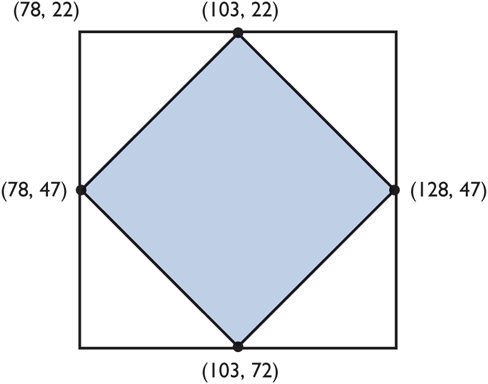
\includegraphics[width=\maxwidth,height=\maxheight,width=0.9\linewidth]{Figures/img_p170_1.png}
\end{center}

Mã để vẽ hình thoi này sẽ là:

\begin{verbatim}
g.drawRect(78, 22, 50, 50);
g.drawLine(78, 47, 103, 22);
g.drawLine(103, 22, 128, 47);
g.drawLine(128, 47, 103, 72);
g.drawLine(103, 72, 78, 47);
\end{verbatim}

Như bạn có thể thấy, các giá trị tham số được truyền cho các phương thức
\texttt{drawRect} và \texttt{drawLine} rất giống với các giá trị của
hình thoi đầu tiên, ngoại trừ việc chúng được dịch chuyển đi 78 theo
hướng \(x\) và 22 theo hướng \(y\) (ngoại trừ tham số thứ ba và thứ tư
của \texttt{drawRect}, vì đây là chiều rộng và chiều cao của hình chữ
nhật). Sự dịch chuyển \texttt{(78,\ 22)} này được gọi là một phần bù
(offset).

Chúng ta có thể tổng quát hóa các tọa độ để truyền vào các lệnh vẽ của
\texttt{Graphics\ g} để chúng hoạt động với bất kỳ hình thoi nào nếu
chúng ta truyền các phần bù \(x\) và \(y\) ở góc trên bên trái của hình
thoi đó. Ví dụ: chúng ta sẽ tổng quát hóa đường thẳng từ
\texttt{(0,\ 25)} trong hình thoi đầu tiên và từ \texttt{(78,\ 47)} đến
\texttt{(103,\ 22)} trong hình thoi thứ hai bằng cách nói rằng đó là một
đường thẳng từ \((x, y + 25)\) đến \((x + 25, y)\), trong đó \((x, y)\)
là phần bù (offset) của hình thoi đã cho.

Chương trình sau đây sử dụng phương thức \texttt{drawDiamond} để vẽ ba
hình thoi mà không bị dư thừa:

\begin{verbatim}
 1  // This program draws several diamond figures of size 50x50.
 2
 3  import java.awt.*;
 4
 5  public class DrawDiamonds {
 6      public static void main(String[] args) {
 7          DrawingPanel panel = new DrawingPanel(250, 150);
 8          Graphics g = panel.getGraphics();
 9
10          drawDiamond(g, 0, 0);
11          drawDiamond(g, 78, 22);
12          drawDiamond(g, 19, 81);
13      }
14
15      // draws a diamond in a 50x50 box
16      public static void drawDiamond(Graphics g, int x, int y) {
17          g.drawRect(x, y, 50, 50);
18          g.drawLine(x, y + 25, x + 25, y);
19          g.drawLine(x + 25, y, x + 50, y + 25);
20          g.drawLine(x + 50, y + 25, x + 25, y + 50);
21          g.drawLine(x + 25, y + 50, x, y + 25);
22      }
23  }
\end{verbatim}

Chương trình này tạo ra đầu ra được hiển thị trong Hình 3G.16.

Hình 3G.16 Đầu ra của \texttt{DrawDiamonds}

\begin{center}

\includegraphics[width=\maxwidth,height=\maxheight,width=0.9\linewidth]{Figures/img_p172_0.png}
\end{center}

Chúng ta có thể vẽ các hình có hoa văn trong các vòng lặp và yêu cầu một
phương thức vẽ gọi một phương thức vẽ khác. Ví dụ: nếu chúng ta muốn vẽ
năm hình thoi, bắt đầu tại tọa độ \texttt{(12,\ 15)} và cách nhau 60
pixel, chúng ta chỉ cần một vòng lặp \texttt{for} lặp lại năm lần và
dịch chuyển tọa độ \(x\) thêm 60 mỗi lần. Đây là một vòng lặp ví dụ:

\begin{verbatim}
for (int i = 0; i < 5; i++) {
    drawDiamond(g, 12 + 60 * i, 15);
}
\end{verbatim}

\begin{center}
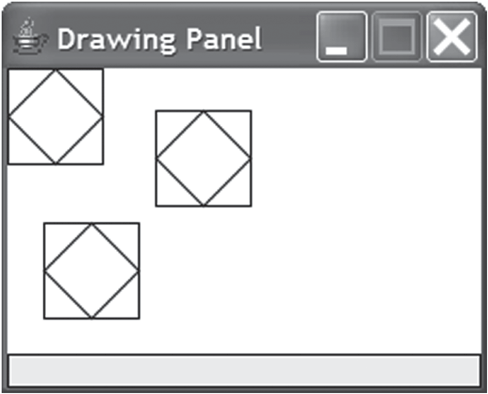
\includegraphics[width=\maxwidth,height=\maxheight,width=0.9\linewidth]{Figures/img_p173_0.png}
\end{center}

Nếu chúng ta tạo một phương thức khác để vẽ đường gồm năm hình thoi,
chúng ta có thể gọi nó từ \texttt{main} để vẽ nhiều đường thẳng chứa các
hình thoi. Dưới đây là phiên bản sửa đổi của chương trình
\texttt{DrawDiamonds} với hai phương thức đồ họa:

\begin{verbatim}
 1  // This program draws several diamond figures of size 50x50.
 2
 3  import java.awt.*;
 4
 5  public class DrawDiamonds2 {
 6      public static void main(String[] args) {
 7          DrawingPanel panel = new DrawingPanel(360, 160);
 8          Graphics g = panel.getGraphics();
 9
10          drawManyDiamonds(g, 12, 15);
11          g.setColor(Color.RED);
12          drawManyDiamonds(g, 55, 100);
13      }
14
15      // draws five diamonds in a horizontal line
16      public static void drawManyDiamonds(Graphics g,
17                                         int x, int y) {
18          for (int i = 0; i < 5; i++) {
19              drawDiamond(g, x + 60 * i, y);
20          }
21      }
22
23      // draws a diamond in a 50x50 box


24      public static void drawDiamond(Graphics g, int x, int y) {
25          g.drawRect(x, y, 50, 50);
26          g.drawLine(x, y + 25, x + 25, y);
27          g.drawLine(x + 25, y, x + 50, y + 25);
28          g.drawLine(x + 50, y + 25, x + 25, y + 50);
29          g.drawLine(x + 25, y + 50, x, y + 25);
30      }
31  }
\end{verbatim}

Chương trình này tạo ra đầu ra được hiển thị trong Hình 3G.17.

Hình 3G.17 Đầu ra của \texttt{DrawDiamonds2}

\begin{center}
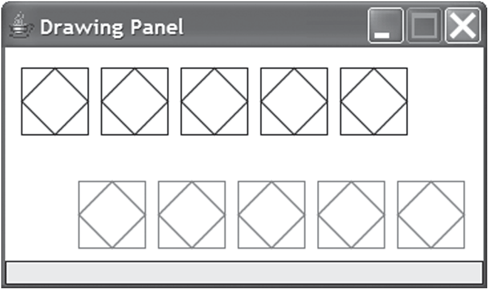
\includegraphics[width=\maxwidth,height=\maxheight,width=0.9\linewidth]{Figures/img_p175_1.png}
\end{center}

\subsection{3G.3 Nghiên cứu điển hình: Kim tự tháp (Case Study:
Pyramids)}\label{g.3-nghiuxean-cux1ee9u-ux111iux1ec3n-huxecnh-kim-tux1ef1-thuxe1p-case-study-pyramids-1}

Hãy tưởng tượng rằng bạn đã được yêu cầu viết một chương trình để vẽ các
hình ảnh trong Hình 3G.18 lên một \texttt{DrawingPanel}.

Hình 3G.18 Đầu ra Kim tự tháp (Pyramids) mong muốn

\begin{center}

\includegraphics[width=\maxwidth,height=\maxheight,width=0.9\linewidth]{Figures/img_p176_1.png}
\end{center}

Bảng vẽ (drawing panel) tổng thể có kích thước là \(350 \times 250\).
Mỗi kim tự tháp cao 100 pixel và rộng 100 pixel. Các kim tự tháp bao gồm
các bậc thang có màu sắc được căn giữa và mở rộng dần về phía dưới, với
các đường viền màu đen xung quanh mỗi bậc thang. Bảng 3G.6 liệt kê các
thuộc tính của từng kim tự tháp.

Bảng 3G.6 Các thuộc tính của Kim tự tháp

\begin{center}
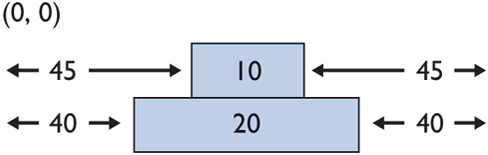
\includegraphics[width=\maxwidth,height=\maxheight,width=0.9\linewidth]{Figures/img_p177_0.png}
\end{center}

\subsubsection{Giải pháp phi cấu trúc một phần (Unstructured Partial
Solution)}\label{giux1ea3i-phuxe1p-phi-cux1ea5u-truxfac-mux1ed9t-phux1ea7n-unstructured-partial-solution}

Khi cố gắng giải quyết một bài toán lớn và phức tạp hơn như bài toán
này, điều quan trọng là phải giải quyết từng phần và cải tiến lặp đi lặp
lại (iterative enhancements) hướng tới một giải pháp hoàn chỉnh. Hãy bắt
đầu bằng cách cố gắng vẽ đúng kim tự tháp màu trắng ở góc trên cùng bên
trái.

Mỗi bậc thang được căn giữa theo chiều ngang trong kim tự tháp. Bậc
thang trên cùng rộng 10 pixel. Do đó, nó được bao quanh bởi \(90/2\)
hoặc 45 pixel khoảng trống ở mỗi bên. Điều đó có nghĩa là góc trên cùng
bên trái của hình chữ nhật \(10 \times 10\) nằm ở tọa độ
\texttt{(45,\ 0)}. Bậc thang thứ hai rộng 20 pixel, có nghĩa là nó được
bao quanh bởi \(80/2\) hoặc 40 pixel ở mỗi bên:

\begin{center}

\includegraphics[width=\maxwidth,height=\maxheight,width=0.9\linewidth]{Figures/img_p177_1.png}
\end{center}

Chương trình sau đây vẽ kim tự tháp màu trắng ở đúng vị trí:

\begin{verbatim}
 1  import java.awt.*;
 2
 3  // Draws the first pyramid only, with a lot of redundancy.
 4  public class Pyramids1 {
 5      public static void main(String[] args) {
 6          DrawingPanel panel = new DrawingPanel(350, 250);
 7          Graphics g = panel.getGraphics();
 8
 9          // draws the border rectangle
10          g.drawRect(0, 0, 100, 100);
11
12          // draws the 10 "stairs" in the white pyramid
13          g.drawRect(45,  0,  10, 10);
14          g.drawRect(40, 10,  20, 10);
15          g.drawRect(35, 20,  30, 10);
16          g.drawRect(30, 30,  40, 10);
17          g.drawRect(25, 40,  50, 10);
18          g.drawRect(20, 50,  60, 10);
19          g.drawRect(15, 60,  70, 10);
20          g.drawRect(10, 70,  80, 10);
21          g.drawRect( 5, 80,  90, 10);
22          g.drawRect( 0, 90, 100, 10);
23      }
24  }
\end{verbatim}

Nhìn vào mã, rõ ràng là có rất nhiều sự dư thừa (redundancy) giữa 10
dòng để vẽ các bậc thang. Kiểm tra các mẫu số trong mỗi cột tiết lộ rằng
giá trị \(x\) giảm đi 5 mỗi lần, giá trị \(y\) tăng thêm 10 mỗi lần,
chiều rộng tăng thêm 10 mỗi lần và chiều cao không đổi.

Một cách khác để mô tả giá trị \(x\) của bậc thang là nói rằng nó bằng
một nửa tổng số 100 trừ đi chiều rộng của bậc thang. Với suy nghĩ đó,
vòng lặp \texttt{for} sau đây vẽ 10 bậc thang mà không có sự lặp lại như
trước đó:

\begin{verbatim}
for (int i = 0; i < 10; i++) {
    int stairWidth = 10 * (i + 1);
    int stairHeight = 10;
    int stairX = (100 - stairWidth) / 2;
    int stairY = 10 * i;
    g.drawRect(stairX, stairY, stairWidth, stairHeight);
}
\end{verbatim}

\subsubsection{Tổng quát hóa việc vẽ các Kim tự tháp (Generalizing the
Drawing of
Pyramids)}\label{tux1ed5ng-quuxe1t-huxf3a-viux1ec7c-vux1ebd-cuxe1c-kim-tux1ef1-thuxe1p-generalizing-the-drawing-of-pyramids}

Tiếp theo, hãy thêm mã để vẽ kim tự tháp (màu đỏ) ở dưới cùng. Vị trí
\((x, y)\) của nó là \texttt{(80,\ 140)} và nó chỉ có năm bậc thang.
Điều đó có nghĩa là mỗi bậc thang

cao và rộng gấp đôi so với các bậc thang trong kim tự tháp màu trắng.

Dựa vào thông tin này, chúng ta có thể xác định rằng góc trên bên trái
của bậc thang trên cùng nằm ở \texttt{(120,\ 140)} và kích thước của nó
là \(20 \times 20\), góc trên bên trái của bậc thang thứ hai nằm ở
\texttt{(110,\ 160)} và kích thước của nó là \(40 \times 20\), và cứ thế
tiếp tục.

Hiện tại, hãy tập trung vào việc lấy đúng tọa độ của các bậc thang và
không lo lắng về màu tô màu đỏ. Dưới đây là một đoạn mã bị dư thừa để vẽ
các bậc thang của kim tự tháp màu đỏ, không có tô màu:

\begin{verbatim}
// draws the border rectangle
g.drawRect(80, 140, 100, 100);
// draws the 5 "stairs" of the red pyramid
g.drawRect(120, 140, 20, 20);
g.drawRect(110, 160, 40, 20);
g.drawRect(100, 180, 60, 20);
g.drawRect( 90, 200, 80, 20);
g.drawRect( 80, 220, 100, 20);
\end{verbatim}

\begin{center}
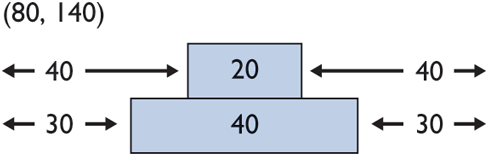
\includegraphics[width=\maxwidth,height=\maxheight,width=0.9\linewidth]{Figures/img_p180_0.png}
\end{center}

Một lần nữa, chúng ta có sự lặp lại giữa năm dòng để vẽ các bậc thang,
vì vậy hãy tìm kiếm một quy luật. Chúng ta sẽ sử dụng một vòng lặp để
loại bỏ sự lặp lại giống như chúng ta đã làm với kim tự tháp trước đó,
nhưng với những sửa đổi thích hợp. Chiều cao của mỗi bậc thang bây giờ
là 20 pixel và chiều rộng của mỗi bậc thang bây giờ là 20 nhân với số
thứ tự của bậc thang đó. Các tọa độ \(x\) và \(y\) khó hơn một chút.
Công thức tính tọa độ \(x\) tương tự như
\texttt{(100\ -\ stairWidth)\ /\ 2} từ trước đó, nhưng lần này nó phải
được dịch sang phải 80 pixel để tính đến vị trí góc trên bên trái của
hộp giới hạn (bounding box). Tọa độ \(y\) tương tự cũng phải được dịch
chuyển xuống dưới 140 pixel. Dưới đây là vòng lặp chính xác:

\begin{verbatim}
// draws the 5 "stairs" of the red pyramid
for (int i = 0; i < 5; i++) {
    int stairWidth = 20 * (i + 1);
    int stairHeight = 20;
    int stairX = 80 + (100 - stairWidth) / 2;
    int stairY = 140 + 20 * i;
    g.drawRect(stairX, stairY, stairWidth, stairHeight);
}
\end{verbatim}

Bạn có thể phát hiện ra quy luật giữa hai vòng lặp \texttt{for} được sử
dụng để vẽ các bậc thang của các kim tự tháp không? Các tọa độ \(x\) và
\(y\) chỉ khác nhau ở việc cộng thêm phần bù (offset) từ
\texttt{(0,\ 0)} trong vòng lặp thứ hai. Chiều rộng và chiều cao của các
bậc thang chỉ khác nhau ở chỗ một bậc thang của kim tự tháp cao 20 pixel
và bậc thang của kim tự tháp kia cao 10 pixel (kết quả của việc lấy tổng
kích thước là 100 chia cho số lượng bậc thang).

Sử dụng thông tin trước đó, hãy biến đoạn mã vẽ kim tự tháp thành một
phương thức mà chúng ta có thể gọi ba lần để tránh sự dư thừa. Các tham
số sẽ là các tọa độ \((x, y)\) của góc trên bên trái của hộp giới hạn
(bounding box) của kim tự tháp và số lượng bậc thang trong kim tự tháp.
Chúng ta cũng sẽ cần truyền \texttt{Graphics\ g} làm tham số để có thể
vẽ lên \texttt{DrawingPanel}. Chúng ta sẽ sửa đổi vòng lặp \texttt{for}
để tính chiều cao của bậc thang trước, sau đó sử dụng chiều cao để tính
chiều rộng của bậc thang và cuối cùng sử dụng chiều rộng và chiều cao để
giúp tính tọa độ \((x, y)\) của bậc thang. Đây là đoạn mã:

\begin{verbatim}
public static void drawPyramid(Graphics g, int x,
                               int y, int stairs) {
    // draws the border rectangle
    g.drawRect(x, y, 100, 100);
    // draws the stairs of the pyramid
    for (int i = 0; i < stairs; i++) {
        int stairHeight = 100 / stairs;
        int stairWidth = stairHeight * (i + 1);
        int stairX = x + (100 - stairWidth) / 2;
        int stairY = y + stairHeight * i;
        g.drawRect(stairX, stairY, stairWidth, stairHeight);
    }
}
\end{verbatim}

Mã trước đó hiện đã được tổng quát hóa để vẽ một kim tự tháp ở bất kỳ vị
trí nào với số lượng bậc thang bất kỳ. Nhưng một yếu tố cuối cùng bị
thiếu: khả năng tạo màu khác nhau cho mỗi kim tự tháp.

\subsubsection{Giải pháp có cấu trúc hoàn chỉnh (Complete Structured
Solution)}\label{giux1ea3i-phuxe1p-cuxf3-cux1ea5u-truxfac-houxe0n-chux1ec9nh-complete-structured-solution}

Đoạn mã trên đúng ngoại trừ việc nó không cho phép chúng ta vẽ các kim
tự tháp với màu sắc thích hợp. Hãy thêm một tham số bổ sung, một đối
tượng \texttt{Color}, vào phương thức của chúng ta và sử dụng nó để tô
màu các bậc thang của kim tự tháp khi cần. Chúng ta sẽ truyền
\texttt{Color.WHITE} làm giá trị của tham số này cho kim tự tháp màu
trắng đầu tiên; nó sẽ tô màu các bậc thang bằng màu trắng, mặc dù điều
này không cần thiết.

Cách để vẽ một hình dạng có màu (filled shape) với một đường viền có màu
khác là tô màu hình dạng đó trước, sau đó sử dụng màu đường viền để vẽ
cùng một hình dạng đó. Ví dụ, để có được các hình chữ nhật màu đỏ có
viền đen, trước tiên chúng ta sẽ sử dụng \texttt{fillRect} với màu đỏ,
sau đó chúng ta sẽ sử dụng \texttt{drawRect} với màu đen cùng với các
tham số tương tự.

Dưới đây là phiên bản mới của phương thức \texttt{drawPyramid} sử dụng
màu tô làm tham số:

\begin{verbatim}
public static void drawPyramid(Graphics g, Color c,
                               int x, int y, int stairs) {
    g.drawRect(x, y, 100, 100);
    for (int i = 0; i < stairs; i++) {
        int stairHeight = 100 / stairs;
        int stairWidth = stairHeight * (i + 1);
        int stairX = x + (100 - stairWidth) / 2;
        int stairY = y + stairHeight * i;
        g.setColor(c);
        g.fillRect(stairX, stairY, stairWidth, stairHeight);
        g.setColor(Color.BLACK);
        g.drawRect(stairX, stairY, stairWidth, stairHeight);
    }
}
\end{verbatim}

Sử dụng phương thức này, giờ đây chúng ta có thể vẽ cả ba kim tự tháp
một cách dễ dàng bằng cách gọi \texttt{drawPyramid} ba lần với các tham
số thích hợp:

\begin{verbatim}
drawPyramid(g, Color.WHITE, 0, 0, 10);
drawPyramid(g, Color.RED, 80, 140, 5);
drawPyramid(g, Color.BLUE, 220, 50, 20);
\end{verbatim}

Một cải tiến cuối cùng mà chúng ta có thể thực hiện cho chương trình
Pyramids của mình là biến kích thước kim tự tháp tổng thể là 100 thành
một hằng số, để không có quá nhiều số 100 nằm rải rác trong mã. Đây là
chương trình hoàn chỉnh:

\begin{verbatim}
 1  // This program draws three colored pyramid figures.
 2
 3  import java.awt.*;
\end{verbatim}

4 5 public class Pyramids \{ 6 public static final int SIZE = 100; 7 8
public static void main(String{[}{]} args) \{ 9 DrawingPanel panel = new
DrawingPanel(350, 250); 10 Graphics g = panel.getGraphics(); 11 12
drawPyramid(g, Color.WHITE, 0, 0, 10); 13 drawPyramid(g, Color.RED, 80,
140, 5); 14 drawPyramid(g, Color.BLUE, 220, 50, 20); 15 \} 16 17 //
draws one pyramid figure with the given 18 // number of stairs at the
given (x, y) position 19 // with the given color 20 public static void
drawPyramid(Graphics g, Color c, 21 int x, int y, int stairs) \{ 22 23
// draws the border rectangle 24 g.drawRect(x, y, SIZE, SIZE); 25 26 //
draws the stairs of the pyramid 27 for (int i = 0; i \textless{} stairs;
i++) \{ 28 int stairHeight = SIZE / stairs; 29 int stairWidth =
stairHeight * (i + 1); 30 int stairX = x + (SIZE - stairWidth) / 2; 31
int stairY = y + stairHeight * i; 32 33 // fills the rectangles with the
fill colors 34 g.setColor(c); 35 g.fillRect(stairX, stairY, stairWidth,
stairHeight); 36 37 // draws the black rectangle outlines 38
g.setColor(Color.BLACK); 39 g.drawRect(stairX, stairY, stairWidth,
stairHeight); 40 \} 41 \} 42 \}

\begin{verbatim}

## Tóm tắt Chương (Chapter Summary)

- `DrawingPanel` là một lớp tùy chỉnh (custom class) được cung cấp bởi các tác giả để dễ dàng hiển thị một cửa sổ đồ họa trên màn hình. Một `DrawingPanel` chứa một đối tượng `Graphics` có thể được sử dụng để vẽ các đường thẳng, văn bản và hình dạng trên màn hình bằng các màu sắc khác nhau.
- Đối tượng `Graphics` có nhiều phương thức hữu ích để vẽ các hình dạng và đường thẳng, chẳng hạn như `drawLine`, `fillRect` và `setColor`. Các hình dạng có thể được "vẽ" ("drawn" - chỉ vẽ đường viền) hoặc "được tô màu" ("filled" - tô màu toàn bộ hình dạng).
- Đối tượng `Graphics` có thể viết văn bản trên màn hình bằng phương thức `drawString` của nó. Bạn có thể chỉ định các kiểu dáng và kích thước phông chữ khác nhau bằng phương thức `setFont`.
- Các chương trình đồ họa được phân rã thành các phương thức phải truyền các tham số thích hợp cho các phương thức đó (ví dụ: đối tượng `Graphics`, cũng như bất kỳ tọa độ $(x, y)$ nào, kích thước hoặc các giá trị khác để hướng dẫn các hình được vẽ).

## Bài tập Tự kiểm tra (Self-Check Problems)

### Phần 3G.1: Giới thiệu về Đồ họa (Introduction to Graphics)

**1.** Cú pháp nào sau đây là đúng để vẽ một hình chữ nhật?
a. `Graphics g.drawRect(10, 20, 50, 30);`
b. `g.drawRect(10, 20, 50, 30);`
c. `g.draw.rectangle(10, 20, 50, 30);`
d. `Graphics.drawRect(10, 20, 50, 30);`
e. `g.drawRect(x = 10, y = 20, width = 50, height = 30);`

**2.** Có hai lỗi trong đoạn mã sau đây, trong đó cố gắng vẽ một đường thẳng từ tọa độ `(50, 86)` đến `(20, 35)`. Chúng là gì?
```java
DrawingPanel panel = new DrawingPanel(200, 200);
panel.drawLine(50, 20, 86, 35);
\end{verbatim}

\textbf{3.} Đoạn mã sau cố gắng vẽ một hình chữ nhật bên ngoài được tô
màu đen với một hình tròn bên trong được tô màu trắng ở trong nó:

\begin{verbatim}
DrawingPanel panel = new DrawingPanel(200, 100);
Graphics g = panel.getGraphics();
g.setColor(Color.WHITE);
g.fillOval(10, 10, 50, 50);
\end{verbatim}

\begin{verbatim}
g.setColor(Color.BLACK);
g.fillRect(10, 10, 50, 50);
\end{verbatim}

Tuy nhiên, đầu ra đồ họa lại trông giống như Hình 3G.19 thay thế. Phải
thay đổi điều gì để nó trông như dự định?

Hình 3G.19 Đầu ra đồ họa của Bài tự kiểm tra (Self-Check) 3G.3

\begin{center}
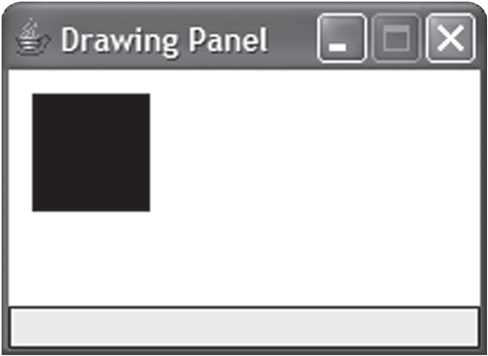
\includegraphics[width=\maxwidth,height=\maxheight,width=0.9\linewidth]{Figures/img_p190_1.png}
\end{center}

\textbf{4.} Đoạn mã sau cố gắng vẽ một hình chữ nhật màu đen từ
\texttt{(10,\ 20)} đến \texttt{(50,\ 40)} với một đường cắt ngang đường
chéo của nó:

\begin{verbatim}
DrawingPanel panel = new DrawingPanel(200, 100);
Graphics g = panel.getGraphics();
g.drawRect(10, 20, 50, 40);
g.drawLine(10, 20, 50, 40);
\end{verbatim}

Tuy nhiên, đầu ra đồ họa lại trông giống như Hình 3G.20 thay thế. Phải
thay đổi điều gì để nó trông như dự định?

Hình 3G.20 Đầu ra đồ họa của Bài tự kiểm tra (Self-Check) 3G.4

\begin{center}
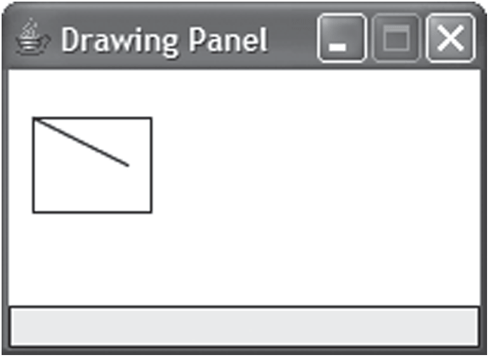
\includegraphics[width=\maxwidth,height=\maxheight,width=0.9\linewidth]{Figures/img_p191_1.png}
\end{center}

\textbf{5.} Loại hình nào sẽ được vẽ bởi chương trình sau? Bạn có thể vẽ
một bức tranh gần giống với hình dạng của nó mà không cần chạy nó trước
không?

\begin{verbatim}
 1  import java.awt.*;
 2
 3  public class Draw7 {
 4      public static void main(String[] args) {
 5          DrawingPanel panel = new DrawingPanel(200, 200);
 6          Graphics g = panel.getGraphics();
 7          for (int i = 0; i < 20; i++) {
 8              g.drawOval(i * 10, i * 10, 200 - (i * 10), 200 - (i * 10));
 9          }
10      }
11  }
\end{verbatim}

\subsection{Bài tập (Exercises)}\label{buxe0i-tux1eadp-exercises}

\textbf{1.} Viết một chương trình sử dụng \texttt{DrawingPanel} để vẽ
Hình 3G.21.

Hình 3G.21 Đầu ra đồ họa mong muốn của Bài tập 3G.1

\begin{center}

\includegraphics[width=\maxwidth,height=\maxheight,width=0.9\linewidth]{Figures/img_p193_1.png}
\end{center}

Cửa sổ rộng 220 pixel và cao 150 pixel. Hình nền màu vàng. Có hai hình
bầu dục màu xanh dương có kích thước \(40 \times 40\) pixel. Chúng cách
nhau 80 pixel, và góc trên bên trái của hình bầu dục bên trái nằm ở vị
trí \texttt{(50,\ 25)}. Có một hình vuông màu đỏ mà hai góc trên của nó
cắt chính xác tâm của hai hình bầu dục. Cuối cùng, có một đường ngang
màu đen đi qua tâm của hình vuông.

\textbf{2.} Sửa đổi chương trình của bạn từ bài tập trước để vẽ hình
bằng một phương thức có tên là \texttt{drawFigure}. Phương thức nên chấp
nhận ba tham số: \texttt{Graphics\ g} của \texttt{DrawingPanel} để vẽ
lên, và một cặp tọa độ \((x, y)\) chỉ định vị trí của góc trên bên trái
của hình. Sử dụng tiêu đề (heading) sau cho phương thức của bạn:

\begin{verbatim}
public static void drawFigure(Graphics g, int x, int y)
\end{verbatim}

Đặt kích thước của \texttt{DrawingPanel} của bạn thành
\(450 \times 150\) pixel và sử dụng phương thức \texttt{drawFigure} của
bạn để đặt hai hình lên đó, như được hiển thị trong Hình 3G.22. Một hình
nên ở vị trí \texttt{(50,\ 25)} và hình kia nên ở vị trí
\texttt{(250,\ 45)}.

Hình 3G.22 Đầu ra đồ họa mong muốn của Bài tập 3G.2

\begin{center}

\includegraphics[width=\maxwidth,height=\maxheight,width=0.9\linewidth]{Figures/img_p194_0.png}
\end{center}

\textbf{3.} Giả sử bạn có chương trình hiện tại sau đây tên là
\texttt{Face}, sử dụng \texttt{DrawingPanel} để vẽ hình khuôn mặt được
hiển thị trong Hình 3G.23. Sửa đổi chương trình để vẽ đầu ra đã được sửa
đổi hiển thị trong Hình 3G.24. Hãy làm như vậy bằng cách viết một phương
thức được tham số hóa (parameterized method) để vẽ một khuôn mặt ở các
vị trí khác nhau. Kích thước cửa sổ nên được thay đổi thành
\(320 \times 180\) pixel, và góc trên bên trái của hai khuôn mặt nằm ở
\texttt{(10,\ 30)} và \texttt{(150,\ 50)}.

Hình 3G.23 Đầu ra đồ họa ban đầu của Bài tập 3G.3

\begin{center}

\includegraphics[width=\maxwidth,height=\maxheight,width=0.9\linewidth]{Figures/img_p195_1.png}
\end{center}

Hình 3G.24 Đầu ra đồ họa mong muốn của Bài tập 3G.3

\begin{center}

\includegraphics[width=\maxwidth,height=\maxheight,width=0.9\linewidth]{Figures/img_p196_1.png}
\end{center}

\begin{verbatim}
 1  public class Face {
 2      public static void main(String[] args) {
 3          DrawingPanel panel = new DrawingPanel(220, 150);
 4          Graphics g = panel.getGraphics();
 5
 6          g.setColor(Color.BLACK);
 7          g.drawOval(10, 30, 100, 100);   // face outline
 8
 9          g.setColor(Color.BLUE);
10          g.fillOval(30, 60, 20, 20);     // eyes
11          g.fillOval(70, 60, 20, 20);
12
13          g.setColor(Color.RED);          // mouth
14          g.drawLine(40, 100, 80, 100);
15      }
16  }
\end{verbatim}

\textbf{4.} Sửa đổi chương trình \texttt{Face} trước đó của bạn để vẽ
đầu ra mới được hiển thị trong Hình 3G.25. Kích thước cửa sổ nên được
thay đổi thành \(520 \times 180\) pixel, và các góc trên bên trái của
các khuôn mặt nằm ở \texttt{(10,\ 30)}, \texttt{(110,\ 30)},
\texttt{(210,\ 30)}, \texttt{(310,\ 30)} và \texttt{(410,\ 30)}.

Hình 3G.25 Đầu ra đồ họa mong muốn của Bài tập 3G.4

\begin{center}

\includegraphics[width=\maxwidth,height=\maxheight,width=0.9\linewidth]{Figures/img_p198_1.png}
\end{center}

\textbf{5.} Viết một chương trình tên là \texttt{ShowDesign} sử dụng
\texttt{DrawingPanel} để vẽ Hình 3G.26.

Hình 3G.26 Đầu ra đồ họa mong muốn của Bài tập 3G.5

\begin{center}
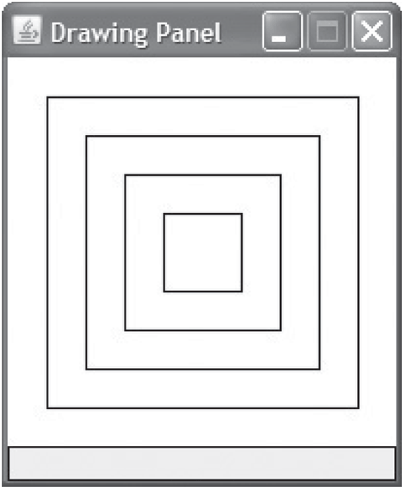
\includegraphics[width=\maxwidth,height=\maxheight,width=0.9\linewidth]{Figures/img_p199_0.png}
\end{center}

Cửa sổ rộng 200 pixel và cao 200 pixel. Màu nền là màu trắng và màu tiền
cảnh là màu đen. Khoảng cách giữa bốn hình chữ nhật là 20 pixel, và các
hình chữ nhật là đồng tâm (tâm của chúng nằm ở cùng một điểm). Sử dụng
vòng lặp để vẽ các hình chữ nhật lặp đi lặp lại.

\textbf{6.} Sửa đổi chương trình \texttt{ShowDesign} của bạn từ bài tập
trước sao cho nó có một phương thức chấp nhận các tham số về chiều rộng
và chiều cao của cửa sổ, và hiển thị các hình chữ nhật ở kích thước phù
hợp. Ví dụ: nếu phương thức của bạn được gọi với các giá trị
\texttt{300} và \texttt{100}, cửa sổ sẽ trông giống như Hình 3G.27.

Hình 3G.27 Đầu ra đồ họa mong muốn của Bài tập 3G.6

\begin{center}
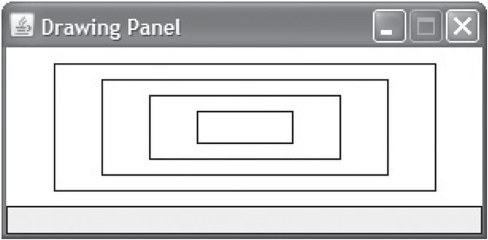
\includegraphics[width=\maxwidth,height=\maxheight,width=0.9\linewidth]{Figures/img_p200_0.png}
\end{center}

\textbf{7.} Viết một chương trình tên là \texttt{Squares} sử dụng
\texttt{DrawingPanel} để vẽ hình dạng hiển thị trong Hình 3G.28.

Hình 3G.28 Đầu ra đồ họa mong muốn của Bài tập 3G.7

\begin{center}

\includegraphics[width=\maxwidth,height=\maxheight,width=0.9\linewidth]{Figures/img_p200_1.png}
\end{center}

\texttt{DrawingPanel} có kích thước rộng 300 pixel và cao 200 pixel.
Hình nền của nó là màu lục lam (cyan). Các đường ngang và dọc được vẽ
bằng màu đỏ và đường chéo được vẽ bằng màu đen. Góc trên bên trái của
đường chéo nằm ở \texttt{(50,\ 50)}. Các đường ngang và dọc liên tiếp
cách nhau 20 pixel.

\textbf{8.} Sửa đổi mã của bạn từ bài tập trước để tạo ra hoa văn được
hiển thị trong Hình 3G.29.

Hình 3G.29 Đầu ra đồ họa mong muốn của Bài tập 3G.8

\begin{center}

\includegraphics[width=\maxwidth,height=\maxheight,width=0.9\linewidth]{Figures/img_p201_1.png}
\end{center}

\texttt{DrawingPanel} bây giờ có kích thước \(400 \times 300\) pixel.
Hình đầu tiên nằm ở vị trí cũ, \texttt{(50,\ 50)}. Các hình khác lần
lượt ở vị trí \texttt{(250,\ 10)} và \texttt{(180,\ 115)}. Sử dụng một
hoặc nhiều phương thức tĩnh có tham số (parameterized static methods) để
giảm sự lặp lại trong giải pháp của bạn.

\textbf{9.} Sửa đổi mã của bạn từ bài tập trước để tạo ra hoa văn được
hiển thị trong Hình 3G.30.

Hình 3G.30 Đầu ra đồ họa mong muốn của Bài tập 3G.9

\begin{center}

\includegraphics[width=\maxwidth,height=\maxheight,width=0.9\linewidth]{Figures/img_p202_1.png}
\end{center}

\texttt{DrawingPanel} giống như bài trước ngoại trừ việc bây giờ mỗi
hình có một kích thước khác nhau. Hình bên trái có kích thước ban đầu là
100, hình trên cùng bên phải có kích thước là 50, và hình dưới cùng bên
phải có kích thước là 180. Sử dụng các phương thức tĩnh có tham số
(parameterized static methods) để giảm sự dư thừa của giải pháp của bạn.

\textbf{10.} Viết một chương trình tên là \texttt{Stairs} sử dụng
\texttt{DrawingPanel} để vẽ hình hiển thị trong Hình 3G.31. Góc trên bên
trái của bậc thang đầu tiên nằm ở vị trí \texttt{(5,\ 5)}. Bậc thang đầu
tiên có kích thước \(10 \times 10\) pixel. Mỗi bậc thang rộng hơn bậc
trên nó 10 pixel. Tạo một bảng gồm các tọa độ \((x, y)\) và kích thước
\((\text{width} \times \text{height})\) của năm bậc thang đầu tiên. Lưu
ý những giá trị nào thay đổi và những giá trị nào không đổi.

Hình 3G.31 Đầu ra đồ họa mong muốn của Bài tập 3G.10

\begin{center}
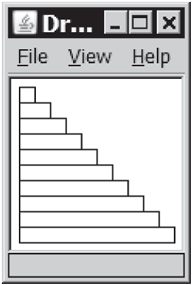
\includegraphics[width=\maxwidth,height=\maxheight,width=0.9\linewidth]{Figures/img_p204_0.png}
\end{center}

\textbf{11.} Sửa đổi chương trình \texttt{Stairs} trước đó của bạn để vẽ
từng đầu ra được hiển thị trong Hình 3G.32. Chỉ sửa đổi phần thân của
vòng lặp của bạn. (Bạn có thể muốn tạo một bảng mới để tìm biểu thức cho
\(x\), \(y\), chiều rộng và chiều cao cho từng đầu ra mới.)

Hình 3G.32 Đầu ra đồ họa mong muốn của Bài tập 3G.11

\begin{center}

\includegraphics[width=\maxwidth,height=\maxheight,width=0.9\linewidth]{Figures/img_p204_1.png}
\end{center}

\textbf{12.} Viết một chương trình tên là \texttt{Triangle} sử dụng
\texttt{DrawingPanel} để vẽ hình hiển thị trong Hình 3G.33.

Hình 3G.33 Đầu ra đồ họa mong muốn của Bài tập 3G.12

\begin{center}

\includegraphics[width=\maxwidth,height=\maxheight,width=0.9\linewidth]{Figures/img_p205_2.png}
\end{center}

Cửa sổ có kích thước \(600 \times 200\) pixel. Nền màu vàng và các đường
vẽ màu xanh dương. Các đường vẽ cách nhau 10 pixel theo chiều dọc và các
đường chéo giao nhau ở dưới cùng của hình, tại chính giữa theo chiều
ngang.

\textbf{13.} Viết một chương trình tên là \texttt{Football} sử dụng
\texttt{DrawingPanel} để vẽ hình hiển thị trong Hình 3G.34. Mặc dù hình
trông có vẻ chứa các đường cong, nhưng nó hoàn toàn được tạo thành từ
các đường thẳng.

Hình 3G.34 Đầu ra đồ họa mong muốn của Bài tập 3G.13

\begin{center}

\includegraphics[width=\maxwidth,height=\maxheight,width=0.9\linewidth]{Figures/img_p206_1.png}
\end{center}

Cửa sổ có kích thước \(250 \times 250\) pixel. Có một hình chữ nhật bên
ngoài từ \texttt{(10,\ 30)} đến \texttt{(210,\ 230)} và một tập hợp các
đường màu đen được vẽ xung quanh các cạnh cách nhau mỗi 10 pixel. Ví dụ:
dọc theo phía trên bên trái có một đường từ \texttt{(10,\ 200)} đến
\texttt{(20,\ 30)}, một đường từ \texttt{(10,\ 190)} đến
\texttt{(30,\ 30)}, một đường từ \texttt{(10,\ 180)} đến
\texttt{(40,\ 30)},\ldots{} và dọc theo phía dưới bên phải có một đường
từ \texttt{(20,\ 210)} đến \texttt{(210,\ 200)}, một đường từ
\texttt{(30,\ 210)} đến \texttt{(210,\ 190)}, v.v.

\subsection{Dự án Lập trình (Programming
Projects)}\label{dux1ef1-uxe1n-lux1eadp-truxecnh-programming-projects-1}

\textbf{1.} Viết một chương trình vẽ các hoa văn hiển thị trong Hình
3G.35 lên một \texttt{DrawingPanel}.

Hình 3G.35 Đầu ra đồ họa mong muốn của Dự án Lập trình 3G.1

\begin{center}

\includegraphics[width=\maxwidth,height=\maxheight,width=0.9\linewidth]{Figures/img_p208_1.png}
\end{center}

Kích thước của \texttt{DrawingPanel} là \(400 \times 400\) pixel và màu
nền của nó là màu lục lam (cyan). Nó chứa bốn hình bao gồm các hình tròn
đồng tâm màu vàng với viền đen, tất cả được bao quanh bởi một hình chữ
nhật màu xanh lá cây có viền đen. Bốn hình trên \texttt{DrawingPanel}
của bạn phải có các thuộc tính được hiển thị trong Bảng 3G.7.

Bảng 3G.7 Các thuộc tính của hình tròn

Chia nhỏ chương trình của bạn thành các phương thức để vẽ một hình con
cũng như các lưới hình con lớn hơn, chẳng hạn như lưới \(5 \times 5\) ở
vị trí \texttt{(10,\ 120)}.

\textbf{2.} Viết một chương trình vẽ hình ảnh được hiển thị trong Hình
3G.36 lên một \texttt{DrawingPanel} có kích thước \(200 \times 200\).
Mỗi con tem (stamp) có kích thước \(50 \times 50\) pixel.

Hình 3G.36 Đầu ra đồ họa mong muốn của Dự án Lập trình 3G.2

\begin{center}

\includegraphics[width=\maxwidth,height=\maxheight,width=0.9\linewidth]{Figures/img_p209_0.png}
\end{center}

\textbf{3.} Viết một chương trình vẽ các bàn cờ (checkerboards) giống
như được hiển thị trong Hình 3G.37 lên một \texttt{DrawingPanel} có kích
thước \(420 \times 300\).

Hình 3G.37 Đầu ra đồ họa mong muốn của Dự án Lập trình 3G.3

\begin{center}

\includegraphics[width=\maxwidth,height=\maxheight,width=0.9\linewidth]{Figures/img_p210_1.png}
\end{center}

\textbf{4.} Viết một phiên bản sửa đổi của chương trình nghiên cứu điển
hình \texttt{Projectile} từ Chương 3 để vẽ một đồ thị về chuyến bay của
đường đạn (projectile's flight) lên một \texttt{DrawingPanel} có kích
thước \(420 \times 220\). Ví dụ, bảng điều khiển được hiển thị trong
Hình 3G.38 vẽ một đường đạn với vận tốc ban đầu là 30 mét mỗi giây, một
góc là 50 độ, và 10 bước.

Hình 3G.38 Đầu ra đồ họa mong muốn của Dự án Lập trình 3G.4

\begin{center}

\includegraphics[width=\maxwidth,height=\maxheight,width=0.9\linewidth]{Figures/img_p211_1.png}
\end{center}

\textbf{5.} Viết một chương trình vẽ hình ảnh được hiển thị trong Hình
3G.39 lên một \texttt{DrawingPanel} có kích thước \(650 \times 400\).
Hình ảnh này đại diện cho một ảo ảnh quang học nổi tiếng được gọi là
``Cafe Wall'', trong đó một loạt các hình vuông thẳng (straight squares)
dường như bị nghiêng.

Hình 3G.39 Đầu ra đồ họa mong muốn của Dự án Lập trình 3G.5

\begin{center}

\includegraphics[width=\maxwidth,height=\maxheight,width=0.9\linewidth]{Figures/img_p212_1.png}
\end{center}

Hình ảnh có nền màu xám và nhiều hàng hình vuông màu đen và màu trắng
với một chữ X màu xanh dương được vẽ xuyên qua mỗi hình vuông màu đen.
Hai hàng đứng tự do (free-standing rows) trong sơ đồ có các thuộc tính
sau:

Bảng 3G.8 Các thuộc tính của hàng Cafe Wall

\begin{center}
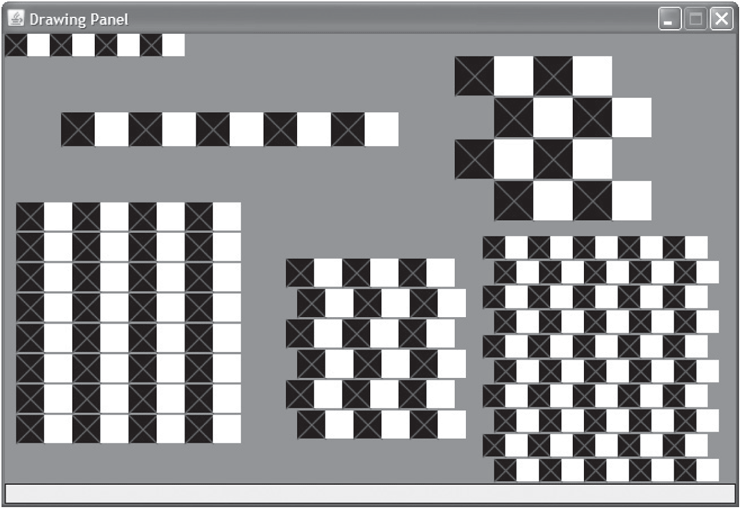
\includegraphics[width=\maxwidth,height=\maxheight,width=0.9\linewidth]{Figures/img_p213_0.png}
\end{center}

Sơ đồ có bốn lưới gồm các hàng hình vuông, với 2 pixel khoảng trống theo
chiều dọc giữa các hàng kề nhau. Một khía cạnh quan trọng của ảo ảnh
quang học là mỗi hàng xen kẽ (every other row) được dịch chuyển theo
chiều ngang bởi một phần bù (offset) cụ thể. Bốn lưới có các thuộc tính
sau:

Bảng 3G.9 Các thuộc tính của lưới Cafe Wall


\providecommand{\pandocbounded}[1]{#1}
\makeatletter
\def\maxwidth{\ifdim\Gin@nat@width>\linewidth\linewidth\else\Gin@nat@width\fi}
\def\maxheight{\ifdim\Gin@nat@height>\textheight\textheight\else\Gin@nat@height\fi}
\makeatother
\providecommand{\tightlist}{\setlength{\itemsep}{0pt}\setlength{\parskip}{0pt}}
\chapter{Lệnh thực thi có điều kiện}
\section{Chương 4 Lệnh thực thi có điều kiện (Conditional
Execution)}\label{chux1b0ux1a1ng-4-lux1ec7nh-thux1ef1c-thi-cuxf3-ux111iux1ec1u-kiux1ec7n-conditional-execution}

\subsection{Lệnh if/else}\label{lux1ec7nh-ifelse}

\begin{itemize}
\tightlist
\item
  Các toán tử quan hệ (Relational Operators)
\item
  Các lệnh if/else lồng nhau (Nested if/else Statements)
\item
  Sự bằng nhau của đối tượng (Object Equality)
\item
  Tối ưu hóa lệnh if/else (Factoring if/else Statements)
\item
  Kiểm tra nhiều điều kiện (Testing Multiple Conditions)
\end{itemize}

\subsection{Các thuật toán tích lũy (Cumulative
Algorithms)}\label{cuxe1c-thuux1eadt-touxe1n-tuxedch-lux169y-cumulative-algorithms}

\begin{itemize}
\tightlist
\item
  Tính tổng tích lũy (Cumulative Sum)
\item
  Vòng lặp tìm Min/Max
\item
  Tính tổng tích lũy với if
\item
  Sai số làm tròn (Roundoff Errors)
\end{itemize}

\subsection{Xử lý văn bản (Text
Processing)}\label{xux1eed-luxfd-vux103n-bux1ea3n-text-processing}

\begin{itemize}
\tightlist
\item
  Kiểu char
\end{itemize}

\begin{center}

\includegraphics[width=\maxwidth,height=\maxheight,width=0.9\linewidth]{Figures/img_p216_0.png}
\end{center}

\begin{itemize}
\tightlist
\item
  char so với int
\item
  Các thuật toán xử lý văn bản tích lũy
\item
  System.out.printf
\end{itemize}

\subsection{Các phương thức có lệnh thực thi có điều
kiện}\label{cuxe1c-phux1b0ux1a1ng-thux1ee9c-cuxf3-lux1ec7nh-thux1ef1c-thi-cuxf3-ux111iux1ec1u-kiux1ec7n}

\begin{itemize}
\tightlist
\item
  Tiền điều kiện và hậu điều kiện (Preconditions and Postconditions)
\item
  Ném ngoại lệ (Throwing Exceptions)
\item
  Xem lại giá trị trả về
\item
  Lập luận về các đường dẫn (Reasoning about Paths)
\end{itemize}

\subsection{Nghiên cứu điển hình: Chỉ số khối cơ thể (Body Mass
Index)}\label{nghiuxean-cux1ee9u-ux111iux1ec3n-huxecnh-chux1ec9-sux1ed1-khux1ed1i-cux1a1-thux1ec3-body-mass-index}

\begin{itemize}
\tightlist
\item
  Giải pháp không có cấu trúc cho một người
\item
  Giải pháp không có cấu trúc cho hai người
\item
  Giải pháp có cấu trúc cho hai người
\item
  Kinh nghiệm thiết kế thủ tục (Procedural Design Heuristics)
\end{itemize}

\subsection{Giới thiệu}\label{giux1edbi-thiux1ec7u}

Trong vài chương trước, bạn đã thấy cách giải quyết các bài toán lập
trình phức tạp bằng cách sử dụng các vòng lặp \texttt{for} để lặp lại
các tác vụ nhất định nhiều lần. Bạn cũng đã thấy cách đưa một số tính
linh hoạt vào các chương trình của mình bằng cách sử dụng các hằng số
lớp (class constants) và cách đọc các giá trị được người dùng nhập bằng
đối tượng \texttt{Scanner}.

\begin{center}

\includegraphics[width=\maxwidth,height=\maxheight,width=0.9\linewidth]{Figures/img_p217_0.png}
\end{center}

Bây giờ, chúng ta sẽ khám phá một kỹ thuật mạnh mẽ hơn nhiều để viết mã
có thể thích ứng với các tình huống khác nhau.

Trong chương này, chúng ta sẽ xem xét việc thực thi có điều kiện
(conditional execution) dưới dạng một cấu trúc điều khiển được gọi là
lệnh \texttt{if/else}. Với các lệnh \texttt{if/else}, bạn có thể hướng
dẫn máy tính thực thi các dòng mã khác nhau tùy thuộc vào việc các điều
kiện nhất định có đúng hay không. Lệnh \texttt{if/else}, giống như vòng
lặp \texttt{for}, mạnh mẽ đến mức bạn sẽ tự hỏi làm thế nào mà bạn xoay
sở viết được các chương trình mà không có nó.

Chương này cũng sẽ mở rộng hiểu biết của bạn về các tình huống lập trình
phổ biến. Nó bao gồm việc khám phá các kỹ thuật vòng lặp mà chúng ta
chưa xem xét và bao gồm cuộc thảo luận về các vấn đề xử lý văn bản. Việc
thêm thực thi có điều kiện vào vốn kiến thức của bạn cũng sẽ yêu cầu
chúng ta xem xét lại các phương thức, tham số và giá trị trả về để bạn
có thể hiểu rõ hơn về một số điểm tinh tế. Chương này kết thúc với một
số quy tắc ngón tay cái (rules of thumb) giúp chúng ta thiết kế các
chương trình thủ tục tốt hơn.

\subsection{Lệnh if/else}\label{lux1ec7nh-ifelse-1}

Bạn sẽ thường thấy mình viết đoạn mã mà bạn muốn thực thi một số lần
nhưng không phải là mọi lúc. Ví dụ, nếu bạn đang viết một chương trình
chơi game, bạn có thể muốn in một thông báo mỗi khi người dùng đạt điểm
cao mới và lưu trữ điểm đó. Bạn có thể hoàn thành việc này bằng cách đặt
hai dòng mã cần thiết bên trong một lệnh \texttt{if}:

\begin{verbatim}
if (currentScore > maxScore) {
    System.out.println("A new high score!");
    maxScore = currentScore;
}
\end{verbatim}

Ý tưởng là đôi khi bạn sẽ muốn thực thi hai dòng mã bên trong lệnh
\texttt{if}, nhưng không phải lúc nào cũng vậy. Biểu thức kiểm tra
(test) trong ngoặc đơn xác định xem các câu lệnh bên trong lệnh
\texttt{if} có được thực thi hay không. Nói cách khác, biểu thức kiểm
tra mô tả các điều kiện mà chúng ta muốn thực thi đoạn mã.

Dạng chung của lệnh \texttt{if} như sau:

\begin{verbatim}
if (<biểu thức kiểm tra>) {
    <câu lệnh>;
    <câu lệnh>;
    ...
    <câu lệnh>;
}
\end{verbatim}

Lệnh \texttt{if}, giống như vòng lặp \texttt{for}, là một cấu trúc điều
khiển. Lưu ý rằng một lần nữa chúng ta lại thấy một từ khóa Java
(\texttt{if}) theo sau là dấu ngoặc đơn và một cặp dấu ngoặc nhọn bao
quanh một chuỗi các câu lệnh được điều khiển.

Sơ đồ trong Hình 4.1 chỉ ra luồng điều khiển của lệnh \texttt{if} đơn
giản. Máy tính thực hiện biểu thức kiểm tra và nếu nó đánh giá là
\texttt{true} (đúng), máy tính sẽ thực thi các câu lệnh được điều khiển.
Nếu biểu thức kiểm tra đánh giá là \texttt{false} (sai), máy tính sẽ bỏ
qua các câu lệnh được điều khiển.

Hình 4.1 Luồng của lệnh \texttt{if}

\begin{center}

\includegraphics[width=\maxwidth,height=\maxheight,width=0.9\linewidth]{Figures/img_p221_0.png}
\end{center}

Bạn sẽ sử dụng lệnh \texttt{if} đơn giản khi bạn có mã mà bạn muốn thực
thi đôi khi và bỏ qua vào những lúc khác. Java cũng có một biến thể được
gọi là lệnh \texttt{if/else} cho phép bạn chọn giữa hai phương án thay
thế. Giả sử, ví dụ, bạn muốn gán biến tên là \texttt{answer} bằng căn
bậc hai của một số:

\begin{verbatim}
answer = Math.sqrt(number);
\end{verbatim}

Bạn không muốn yêu cầu căn bậc hai nếu số đó là số âm. Để tránh sự cố
tiềm ẩn này, bạn có thể sử dụng một lệnh \texttt{if} đơn giản:

\begin{center}
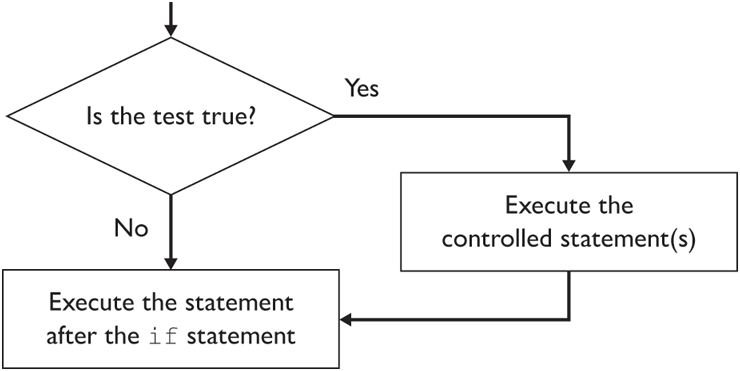
\includegraphics[width=\maxwidth,height=\maxheight,width=0.9\linewidth]{Figures/img_p222_0.png}
\end{center}

\begin{verbatim}
if (number >= 0) {
    answer = Math.sqrt(number);
}
\end{verbatim}

Đoạn mã này sẽ tránh việc yêu cầu căn bậc hai của một số âm, nhưng nó sẽ
gán giá trị gì cho \texttt{answer} nếu \texttt{number} là số âm? Trong
trường hợp này, có lẽ bạn sẽ muốn gán một giá trị cho \texttt{answer}
theo cách này hay cách khác. Giả sử bạn muốn \texttt{answer} là
\texttt{-1} khi \texttt{number} là số âm. Bạn có thể diễn đạt cặp phương
án thay thế này bằng lệnh \texttt{if/else} sau:

\begin{verbatim}
if (number >= 0) {
    answer = Math.sqrt(number);
} else {
    answer = -1;
}
\end{verbatim}

Lệnh \texttt{if/else} cung cấp hai phương án thay thế và thực thi một
hoặc phương án kia. Vì vậy, trong đoạn mã trên, bạn biết rằng
\texttt{answer} sẽ được gán một giá trị bất kể \texttt{number} dương hay
âm.

Dạng chung của lệnh \texttt{if/else} là:

\begin{verbatim}
if (<biểu thức kiểm tra>) {
    <câu lệnh>;
    <câu lệnh>;
    ...
    <câu lệnh>;
} else {
    <câu lệnh>;
    <câu lệnh>;
    ...
    <câu lệnh>;
}
\end{verbatim}

Cấu trúc điều khiển này khác thường ở chỗ nó có hai tập hợp các câu lệnh
được điều khiển và hai từ khóa khác nhau (\texttt{if} và \texttt{else}).
Hình 4.2 chỉ ra luồng điều khiển. Máy tính thực hiện biểu thức kiểm tra
và tùy thuộc vào việc mã đánh giá là \texttt{true} hay \texttt{false},
nó sẽ thực thi một trong hai nhóm câu lệnh.

Hình 4.2 Luồng của lệnh \texttt{if/else}

\begin{center}

\includegraphics[width=\maxwidth,height=\maxheight,width=0.9\linewidth]{Figures/img_p224_0.png}
\end{center}

Cũng giống như trường hợp của vòng lặp \texttt{for}, nếu bạn có một câu
lệnh duy nhất để thực thi, bạn không cần phải bao gồm dấu ngoặc nhọn.
Tuy nhiên, quy ước của Java là bao gồm các dấu ngoặc nhọn ngay cả khi
bạn không cần chúng, và chúng tôi tuân theo quy ước đó trong cuốn sách
này.

\subsubsection{Các toán tử quan hệ (Relational
Operators)}\label{cuxe1c-touxe1n-tux1eed-quan-hux1ec7-relational-operators}

Một lệnh \texttt{if/else} được điều khiển bởi một biểu thức kiểm tra
(test). Các biểu thức kiểm tra đơn giản so sánh hai biểu thức để xem
liệu chúng có liên quan theo một cách nào đó không. Bản thân các biểu
thức kiểm tra như vậy là các biểu thức có dạng sau đây và đánh giá thành
\texttt{true} hoặc \texttt{false}:

\texttt{\textless{}biểu\ thức\textgreater{}\ \textless{}toán\ tử\ quan\ hệ\textgreater{}\ \textless{}biểu\ thức\textgreater{}}

\begin{center}
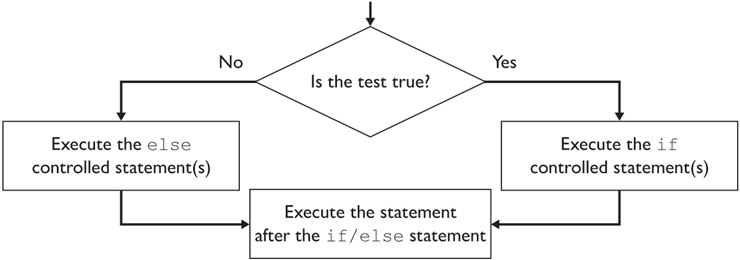
\includegraphics[width=\maxwidth,height=\maxheight,width=0.9\linewidth]{Figures/img_p225_0.png}
\end{center}

Để đánh giá một biểu thức kiểm tra có dạng này, trước tiên hãy đánh giá
hai biểu thức, sau đó xem liệu quan hệ đã cho có thỏa mãn (holds) giữa
giá trị bên trái và giá trị bên phải hay không. Nếu quan hệ thỏa mãn,
biểu thức kiểm tra đánh giá thành \texttt{true}. Nếu không, biểu thức
kiểm tra đánh giá thành \texttt{false}.

Các toán tử quan hệ được liệt kê trong Bảng 4.1. Lưu ý rằng toán tử bằng
(equality operator) bao gồm hai dấu bằng (\texttt{==}), để phân biệt nó
với toán tử gán (assignment operator) (\texttt{=}).

Bảng 4.1 Các toán tử quan hệ

\begin{center}

\includegraphics[width=\maxwidth,height=\maxheight,width=0.9\linewidth]{Figures/img_p226_0.png}
\end{center}

Bởi vì chúng ta sử dụng các toán tử quan hệ như một cách mới để tạo
thành các biểu thức, chúng ta phải xem xét lại độ ưu tiên (precedence).
Bảng 4.2 là phiên bản cập nhật của Bảng 2.5 bao gồm các toán tử mới này.
Bạn sẽ thấy rằng, về mặt kỹ thuật, các phép so sánh bằng có mức độ ưu
tiên hơi khác so với các toán tử quan hệ khác, nhưng cả hai nhóm toán tử
đều có độ ưu tiên thấp hơn các toán tử số học.

Bảng 4.2 Độ ưu tiên của các toán tử trong Java

Hãy xem xét một ví dụ. Biểu thức sau đây được tạo thành từ các hằng số
\texttt{3}, \texttt{2}, và \texttt{9} và chứa các phép tính cộng, nhân,
và phép toán bằng:

\begin{verbatim}
3 + 2 * 2 == 9
\end{verbatim}

\begin{center}
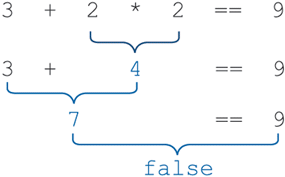
\includegraphics[width=\maxwidth,height=\maxheight,width=0.9\linewidth]{Figures/img_p227_0.png}
\end{center}

Phép toán nào được thực hiện trước? Vì các toán tử quan hệ có mức độ ưu
tiên thấp hơn các toán tử số học, phép nhân được thực hiện trước, sau đó
là phép cộng, sau đó là biểu thức kiểm tra bằng. Nói cách khác, Java sẽ
thực hiện tất cả các phép toán ``toán học'' trước khi nó kiểm tra bất kỳ
mối quan hệ nào. Lược đồ độ ưu tiên này giải phóng bạn khỏi việc phải
đặt dấu ngoặc đơn quanh các vế trái và vế phải của một biểu thức kiểm
tra sử dụng toán tử quan hệ. Khi bạn tuân theo các quy tắc độ ưu tiên
của Java, biểu thức mẫu được đánh giá như sau:

Bạn có thể đặt các biểu thức tùy ý ở hai bên của toán tử quan hệ, miễn
là các kiểu dữ liệu tương thích. Dưới đây là một biểu thức kiểm tra với
các biểu thức phức tạp ở cả hai bên:

\begin{verbatim}
(2 - 3 * 8) / (435 % (7 * 2)) <= 3.8 - 4.5 / (2.2 * 3.8)
\end{verbatim}

Bạn có thể kiểm tra các toán tử quan hệ trong JShell, như được hiển thị
trong tương tác sau:

\begin{verbatim}
jshell> int a = 3; 
a ==> 3
jshell> int b = 2;
b ==> 2
jshell> a > b
$3 ==> true
jshell> a > b * b
$4 ==> false
jshell> a - 1 == b
$5 ==> true
\end{verbatim}

Một hạn chế của các toán tử quan hệ là chúng chỉ nên được sử dụng với dữ
liệu nguyên thủy (primitive data). Ở phần sau của chương này, chúng ta
sẽ nói về cách so sánh sự bằng nhau của các đối tượng (objects) và trong
chương sau, chúng ta sẽ thảo luận về cách thực hiện các phép so sánh nhỏ
hơn và lớn hơn đối với các đối tượng.

\subsubsection{Các lệnh if/else lồng nhau (Nested if/else
Statements)}\label{cuxe1c-lux1ec7nh-ifelse-lux1ed3ng-nhau-nested-ifelse-statements}

\begin{center}

\includegraphics[width=\maxwidth,height=\maxheight,width=0.9\linewidth]{Figures/img_p229_0.png}
\end{center}

Nhiều người mới bắt đầu thường viết mã trông như thế này:

\begin{verbatim}
if (<biểu thức kiểm tra 1>) {
    <câu lệnh 1>;
}
if (<biểu thức kiểm tra 2>) {
    <câu lệnh 2>;
}
if (<biểu thức kiểm tra 3>) {
    <câu lệnh 3>;
}
\end{verbatim}

Cấu trúc tuần tự này phù hợp nếu bạn muốn thực thi bất kỳ tổ hợp nào của
ba câu lệnh. Ví dụ, bạn có thể viết đoạn mã này trong một chương trình
cho một bảng câu hỏi với ba phần tùy chọn, bất kỳ tổ hợp nào trong số đó
cũng có thể áp dụng cho một người cụ thể. Hình 4.3 cho thấy luồng của mã
\texttt{if} tuần tự. Lưu ý rằng máy tính có thể không thực thi câu lệnh
được điều khiển nào (nếu tất cả các biểu thức kiểm tra đều là
\texttt{false}), chỉ thực thi một câu lệnh (nếu tình cờ chỉ có một biểu
thức kiểm tra là \texttt{true}), hoặc thực thi nhiều hơn một câu lệnh
(nếu nhiều biểu thức kiểm tra là \texttt{true}).

Hình 4.3 Luồng của các lệnh \texttt{if} tuần tự (sequential ifs)

\begin{center}

\includegraphics[width=\maxwidth,height=\maxheight,width=0.9\linewidth]{Figures/img_p229_1.png}
\end{center}

\begin{center}
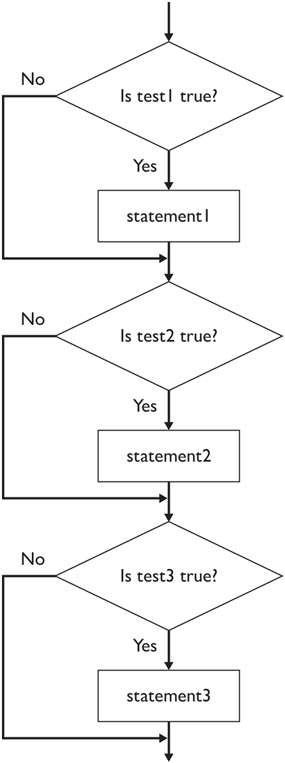
\includegraphics[width=\maxwidth,height=\maxheight,width=0.9\linewidth]{Figures/img_p231_0.png}
\end{center}

Tuy nhiên, thông thường bạn chỉ muốn thực thi một trong một chuỗi các
câu lệnh. Trong những trường hợp như vậy, tốt hơn là lồng các lệnh
\texttt{if}, xếp chúng cái này bên trong cái kia:

\begin{verbatim}
if (<biểu thức kiểm tra 1>) {
    <câu lệnh 1>;
} else {
    if (<biểu thức kiểm tra 2>) {
        <câu lệnh 2>;
    } else {
        if (<biểu thức kiểm tra 3>) {
            <câu lệnh 3>;
        }
    }
}
\end{verbatim}

Khi bạn sử dụng cấu trúc này, bạn có thể chắc chắn rằng máy tính sẽ thực
thi nhiều nhất một câu lệnh: câu lệnh tương ứng với biểu thức kiểm tra
đầu tiên đánh giá thành \texttt{true}. Nếu không có biểu thức kiểm tra
nào đánh giá thành \texttt{true}, không có câu lệnh nào được thực thi.
Nếu mục tiêu của bạn là thực thi nhiều nhất một câu lệnh, cấu trúc này
thích hợp hơn so với các lệnh \texttt{if} tuần tự. Nó làm giảm khả năng
xảy ra lỗi và đơn giản hóa quá trình kiểm thử.

Như bạn có thể thấy, việc lồng các lệnh \texttt{if} như thế này dẫn đến
rất nhiều thụt lề (indentation). Việc thụt lề này không hữu ích lắm, vì
cấu trúc này thực sự nhằm mục đích cho phép chọn một trong nhiều phương
án thay thế. Phong cách K\&R cũng có một giải pháp cho việc này. Nếu một
\texttt{else} được theo sau bởi một \texttt{if}, chúng ta đặt chúng trên
cùng một dòng:

\begin{verbatim}
if (<biểu thức kiểm tra 1>) {
    <câu lệnh 1>;
} else if (<biểu thức kiểm tra 2>) {
    <câu lệnh 2>;
} else if (<biểu thức kiểm tra 3>) {
    <câu lệnh 3>;
}
\end{verbatim}

Khi bạn tuân theo quy ước này, tất cả các câu lệnh khác nhau đều xuất
hiện ở cùng một mức thụt lề. Chúng tôi khuyên bạn nên thụt lề các lệnh
\texttt{if/else} lồng nhau theo cách này.

Hình 4.4 cho thấy luồng của mã \texttt{if/else} lồng nhau. Lưu ý rằng
máy tính có thể thực thi một trong các câu lệnh được điều khiển (câu
lệnh đầu tiên đánh giá thành \texttt{true}) hoặc không thực thi câu lệnh
nào (nếu không có biểu thức kiểm tra nào đánh giá thành \texttt{true}).

Hình 4.4 Luồng của các lệnh \texttt{if} lồng nhau kết thúc bằng biểu
thức kiểm tra (ending in test)

\begin{center}

\includegraphics[width=\maxwidth,height=\maxheight,width=0.9\linewidth]{Figures/img_p233_0.png}
\end{center}

Trong một biến thể của cấu trúc này, câu lệnh cuối cùng được điều khiển
bởi một \texttt{else} thay vì một biểu thức kiểm tra:

\begin{verbatim}
if (<biểu thức kiểm tra 1>) {
    <câu lệnh 1>;
} else if (<biểu thức kiểm tra 2>) {
    <câu lệnh 2>;
\end{verbatim}

\begin{center}
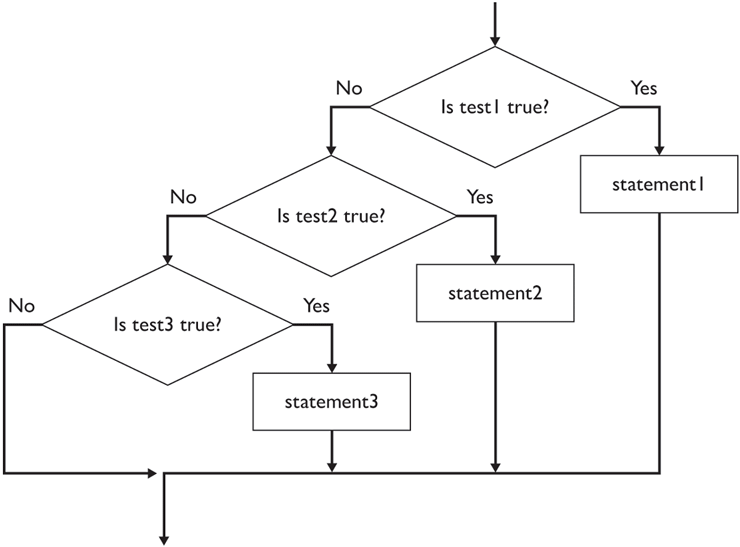
\includegraphics[width=\maxwidth,height=\maxheight,width=0.9\linewidth]{Figures/img_p234_0.png}
\end{center}

\begin{verbatim}
} else {
    <câu lệnh 3>;
}
\end{verbatim}

Trong cấu trúc này, máy tính sẽ luôn chọn nhánh cuối cùng khi tất cả các
biểu thức kiểm tra đều sai, và do đó cấu trúc sẽ luôn thực thi chính xác
một trong ba câu lệnh. Hình 4.5 cho thấy luồng của mã \texttt{if/else}
lồng nhau đã được sửa đổi này.

Hình 4.5 Luồng của các lệnh \texttt{if} lồng nhau kết thúc bằng
\texttt{else}

\begin{center}

\includegraphics[width=\maxwidth,height=\maxheight,width=0.9\linewidth]{Figures/img_p235_0.png}
\end{center}

\begin{center}
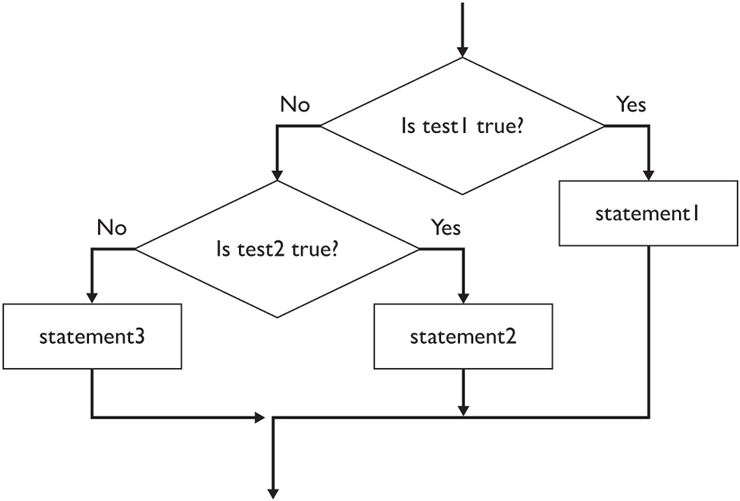
\includegraphics[width=\maxwidth,height=\maxheight,width=0.9\linewidth]{Figures/img_p235_1.png}
\end{center}

Để khám phá những biến thể này, hãy xem xét tác vụ yêu cầu máy tính cho
biết một số là dương, âm, hay bằng 0. Bạn có thể cấu trúc tác vụ này
thành ba lệnh \texttt{if} đơn giản như sau:

\begin{verbatim}
if (number > 0) {
    System.out.println("Number is positive.");
}
if (number == 0) {
    System.out.println("Number is zero.");
}
if (number < 0) {
    System.out.println("Number is negative.");
}
\end{verbatim}

Để xác định có bao nhiêu câu lệnh \texttt{println} có khả năng được thực
thi, bạn phải dừng lại và suy nghĩ về các biểu thức kiểm tra đang được
thực hiện. Nhưng bạn không nên phải tốn nhiều công sức như vậy để hiểu
mã này. Mã sẽ rõ ràng hơn nếu bạn lồng các lệnh \texttt{if}:

\begin{verbatim}
if (number > 0) {
    System.out.println("Number is positive.");
} else if (number == 0) {
    System.out.println("Number is zero.");
} else if (number < 0) {
    System.out.println("Number is negative.");
}
\end{verbatim}

Tuy nhiên, giải pháp này có một vấn đề. Bạn biết rằng bạn muốn thực thi
một và chỉ một câu lệnh \texttt{println}, nhưng cấu trúc lồng nhau này
không loại trừ khả năng không có câu lệnh nào được thực thi (điều này sẽ
xảy ra nếu cả ba biểu thức kiểm tra đều sai). Tất nhiên, với các biểu
thức kiểm tra cụ thể này thì điều đó sẽ không bao giờ xảy ra: Nếu một số
không phải là dương cũng không phải là 0, thì nó phải là âm. Do đó, biểu
thức kiểm tra cuối cùng ở đây là không cần thiết và gây hiểu lầm. Bạn
phải suy nghĩ về các biểu thức kiểm tra để xác định liệu có thể tất cả
ba biểu thức kiểm tra đều sai và cả ba nhánh đều bị bỏ qua hay không.

Trong trường hợp này, giải pháp tốt nhất là phương pháp tiếp cận
\texttt{if/else} lồng nhau với một nhánh cuối cùng luôn được chọn nếu
hai biểu thức kiểm tra đầu tiên đều sai:

\begin{verbatim}
if (number > 0) {
    System.out.println("Number is positive.");
} else if (number == 0) {
    System.out.println("Number is zero.");
} else {
    System.out.println("Number is negative.");
}
\end{verbatim}

Bạn có thể nhìn lướt qua cấu trúc này và thấy ngay rằng chính xác một
câu lệnh \texttt{println} sẽ được thực thi. Bạn không cần phải nhìn vào
các biểu thức kiểm tra đang được thực hiện để nhận ra điều này; đó là
thuộc tính của loại cấu trúc \texttt{if/else} lồng nhau này. Nếu muốn,
bạn có thể bao gồm một chú thích để làm rõ điều gì đang diễn ra:

\begin{verbatim}
if (number > 0) {
    System.out.println("Number is positive.");
} else if (number == 0) {
    System.out.println("Number is zero.");
} else { // number must be negative 
    System.out.println("Number is negative.");
}
\end{verbatim}

Một lợi ích cuối cùng của phương pháp này là tính hiệu quả (efficiency).
Khi mã bao gồm ba lệnh \texttt{if} đơn giản, máy tính sẽ luôn thực hiện
cả ba bài kiểm tra. Khi mã sử dụng phương pháp \texttt{if/else} lồng
nhau, máy tính chỉ thực hiện các biểu thức kiểm tra cho đến khi tìm thấy
sự trùng khớp, điều này là việc sử dụng tài nguyên tốt hơn. Ví dụ, trong
đoạn mã trước, chúng ta chỉ cần thực hiện một bài kiểm tra cho các số
dương và nhiều nhất là hai bài kiểm tra tổng thể.

Khi bạn thấy mình đang viết mã để chọn giữa các phương án thay thế như
thế này, bạn phải phân tích bài toán cụ thể để tìm ra bạn muốn thực thi
có khả năng bao nhiêu nhánh. Nếu việc kết hợp các nhánh nào được chọn
không quan trọng, hãy sử dụng các lệnh \texttt{if} tuần tự. Nếu bạn muốn
chọn một hoặc không chọn nhánh nào, hãy sử dụng các lệnh
\texttt{if/else} lồng nhau với một biểu thức kiểm tra cho mỗi câu lệnh.
Nếu bạn muốn chọn chính xác một nhánh, hãy sử dụng các lệnh
\texttt{if/else} lồng nhau với một nhánh cuối cùng được điều khiển bởi
một \texttt{else} thay vì một biểu thức kiểm tra. Bảng 4.3 tóm tắt những
lựa chọn này.

Bảng 4.3 Các tùy chọn if/else

\begin{center}

\includegraphics[width=\maxwidth,height=\maxheight,width=0.9\linewidth]{Figures/img_p239_0.png}
\end{center}

\subsubsection{LỖI LẬP TRÌNH PHỔ
BIẾN}\label{lux1ed7i-lux1eadp-truxecnh-phux1ed5-biux1ebfn}

\paragraph{Chọn sai cấu trúc
if/else}\label{chux1ecdn-sai-cux1ea5u-truxfac-ifelse}

Giả sử giáo viên của bạn nói rằng điểm số sẽ được xác định như sau: A
cho điểm \textgreater= 90 B cho điểm \textgreater= 80 C cho điểm
\textgreater= 70 D cho điểm \textgreater= 60 F cho điểm \textless{} 60

Bạn có thể chuyển đổi thang điểm này thành mã như sau:

\begin{verbatim}
String grade;
if (score >= 90) {
    grade = "A";
}
if (score >= 80) {
    grade = "B";
}
if (score >= 70) {
    grade = "C";
}
if (score >= 60) {
    grade = "D";
}
if (score < 60) {
    grade = "F";
}
\end{verbatim}

Tuy nhiên, nếu sau đó bạn cố gắng sử dụng biến \texttt{grade} sau đoạn
mã này, bạn sẽ nhận được lỗi này từ trình biên dịch:
\texttt{variable\ grade\ might\ not\ have\ been\ initialized} Đây là một
manh mối cho thấy có một vấn đề. Trình biên dịch Java đang nói rằng nó
tin rằng có những đường dẫn qua mã này sẽ khiến biến \texttt{grade}
không được khởi tạo. Thực tế, biến sẽ luôn được khởi tạo, nhưng trình
biên dịch không thể tìm ra điều này. Chúng ta có thể sửa vấn đề này bằng
cách cung cấp một giá trị ban đầu cho \texttt{grade}:

\begin{verbatim}
String grade = "no grade";
\end{verbatim}

Sự thay đổi này cho phép mã biên dịch được. Nhưng nếu bạn biên dịch và
chạy chương trình, bạn sẽ thấy rằng nó chỉ đưa ra hai mức điểm: D và F.
Bất kỳ ai có điểm số từ 60 trở lên đều nhận được điểm D và bất kỳ ai có
điểm số dưới 60 đều nhận được điểm F. Và mặc dù trình biên dịch phàn nàn
rằng có một đường dẫn có thể khiến \texttt{grade} không được khởi tạo,
nhưng không ai bao giờ nhận được mức điểm là ``no grade''.

Vấn đề ở đây là bạn muốn thực thi chính xác một trong các câu lệnh gán,
nhưng khi bạn sử dụng các lệnh \texttt{if} tuần tự, chương trình có thể
thực thi lần lượt một vài lệnh trong số chúng. Ví dụ, nếu một sinh viên
có điểm số là 95, điểm của sinh viên đó được đặt thành \texttt{"A"}, sau
đó đặt lại thành \texttt{"B"}, sau đó đặt lại thành \texttt{"C"}, và
cuối cùng đặt lại thành \texttt{"D"}. Bạn có thể sửa vấn đề này bằng
cách sử dụng cấu trúc \texttt{if/else} lồng nhau:

\begin{verbatim}
String grade;
if (score >= 90) {
    grade = "A";
} else if (score >= 80) {
     grade = "B";
} else if (score >= 70) {
    grade = "C";
} else if (score >= 60) {
    grade = "D";
} else { // score < 60
    grade = "F";
}
\end{verbatim}

Bây giờ bạn không cần phải đặt \texttt{grade} thành \texttt{"no\ grade"}
vì trình biên dịch có thể thấy rằng bất kể đường dẫn nào được theo sau,
biến \texttt{grade} sẽ được gán một giá trị (chính xác một trong các
nhánh sẽ được thực thi).

\subsubsection{Sự bằng nhau của đối tượng (Object
Equality)}\label{sux1ef1-bux1eb1ng-nhau-cux1ee7a-ux111ux1ed1i-tux1b0ux1ee3ng-object-equality}

Ở phần trước trong chương này, bạn đã thấy rằng bạn có thể sử dụng các
toán tử \texttt{==} và \texttt{!=} để kiểm tra sự bằng nhau và không
bằng nhau tương ứng của dữ liệu nguyên thủy (primitive data). Thật không
may, các toán tử này không hoạt động theo cách bạn có thể mong đợi khi
bạn kiểm tra sự bằng nhau của các đối tượng như chuỗi (strings). Bạn sẽ
phải học một cách mới để kiểm tra sự bằng nhau của các đối tượng.

Ví dụ, bạn có thể viết mã như sau để đọc một token từ bảng điều khiển
(console) và gọi một trong hai phương thức khác nhau tùy thuộc vào việc
người dùng đã trả lời bằng ``yes'' hay ``no''. Nếu người dùng không nhập
từ nào, đoạn mã này được cho là sẽ in ra một thông báo lỗi:

\begin{verbatim}
System.out.print("yes or no? ");
String s = console.next();
if (s == "yes") {
    processYes();
} else if (s == "no") {
    processNo();
} else {
    System.out.println("You didn't type yes or no");
}
\end{verbatim}

Thật không may, đoạn mã này không hoạt động. Bất kể người dùng nhập gì,
chương trình này luôn in ra ``You didn't type yes or no''. Chúng ta sẽ
khám phá chi tiết trong Chương 8 lý do tại sao mã này không hoạt động.
Hiện tại, điều quan trọng cần biết là Java cung cấp một cách thứ hai để
kiểm tra sự bằng nhau dành cho việc sử dụng với các đối tượng. Mọi đối
tượng Java đều có một phương thức được gọi là \texttt{equals} nhận một
đối tượng khác làm đối số. Bạn có thể sử dụng phương thức này để hỏi một
đối tượng xem nó có bằng một đối tượng khác không. Ví dụ, chúng xuất
hiện trong sửa đoạn mã trước đó như sau:

\begin{center}

\includegraphics[width=\maxwidth,height=\maxheight,width=0.9\linewidth]{Figures/img_p243_0.png}
\end{center}

\begin{verbatim}
System.out.print("yes or no? ");
String s = console.next();
if (s.equals("yes")) {
    processYes();
} else if (s.equals("no")) {
    processNo();
} else {
    System.out.println("You didn't type yes or no");
}
\end{verbatim}

Hãy nhớ rằng khi bạn làm việc với chuỗi, bạn phải luôn gọi phương thức
\texttt{equals} thay vì sử dụng \texttt{==}.

Lớp \texttt{String} cũng có một biến thể đặc biệt của phương thức
\texttt{equals} có tên là \texttt{equalsIgnoreCase} để bỏ qua sự khác
biệt về chữ hoa chữ thường (uppercase so với lowercase). Ví dụ, bạn có
thể viết lại đoạn mã trước đó như sau để nhận dạng các phản hồi như
``Yes,'' ``YES,'' ``No,'' ``NO,'' ``yES'', và vân vân:

\begin{verbatim}
System.out.print("yes or no? ");
String s = console.next();
if (s.equalsIgnoreCase("yes")) {
    processYes();
} else if (s.equalsIgnoreCase("no")) {
    processNo();
} else {
    System.out.println("You didn't type yes or no");
}
\end{verbatim}

\subsubsection{Tối ưu hóa lệnh if/else (Factoring if/else
Statements)}\label{tux1ed1i-ux1b0u-huxf3a-lux1ec7nh-ifelse-factoring-ifelse-statements}

Giả sử bạn đang viết một chương trình chơi trò cá cược với người dùng và
bạn muốn đưa ra các cảnh báo khác nhau về số tiền mặt mà người dùng còn
lại. Cấu trúc \texttt{if/else} lồng nhau dưới đây phân biệt ba trường
hợp khác nhau: tiền ít hơn \$500, được coi là thấp; tiền từ \$500 đến
\$1000, được coi là ổn; và tiền trên \$1000, được coi là tốt. Lưu ý rằng
người dùng được đưa ra những lời khuyên khác nhau trong từng trường hợp:

\begin{center}

\includegraphics[width=\maxwidth,height=\maxheight,width=0.9\linewidth]{Figures/img_p245_0.png}
\end{center}

\begin{verbatim}
if (money < 500) {
    System.out.println("You have $" + money + " left.");
    System.out.print("Cash is dangerously low. Bet carefully.");
    System.out.print("How much do you want to bet? ");
    bet = console.nextInt();
} else if (money < 1000) {
    System.out.println("You have $" + money + " left.");
    System.out.print("Cash is somewhat low. Bet moderately.");
    System.out.print("How much do you want to bet? ");
    bet = console.nextInt();
} else {
\end{verbatim}

\begin{verbatim}
    System.out.println("You have $" + money + " left.");
    System.out.print("Cash is in good shape. Bet liberally.");
    System.out.print("How much do you want to bet? ");
    bet = console.nextInt();
}
\end{verbatim}

Cấu trúc này bị lặp lại và có thể được làm hiệu quả hơn bằng cách sử
dụng một kỹ thuật gọi là tối ưu hóa (factoring). Sử dụng kỹ thuật đơn
giản này, bạn rút các đoạn mã chung ra khỏi các nhánh khác nhau của cấu
trúc \texttt{if/else}. Trong đoạn mã trước, ba nhánh khác nhau có thể
thực thi, tùy thuộc vào giá trị của biến \texttt{money}. Bắt đầu bằng
cách viết ra chuỗi các hành động được thực hiện trong mỗi nhánh và so
sánh chúng, như trong Hình 4.6.

Hình 4.6 Các nhánh \texttt{if/else} trước khi tối ưu hóa

\begin{center}

\includegraphics[width=\maxwidth,height=\maxheight,width=0.9\linewidth]{Figures/img_p246_0.png}
\end{center}

\begin{center}
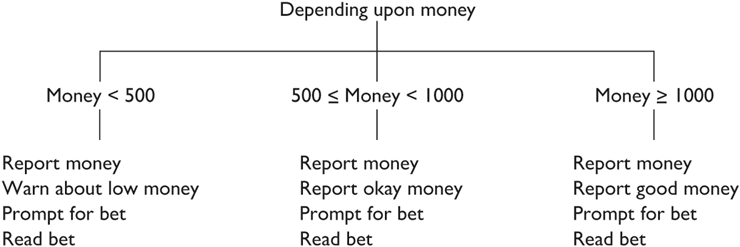
\includegraphics[width=\maxwidth,height=\maxheight,width=0.9\linewidth]{Figures/img_p246_1.png}
\end{center}

Bạn có thể tối ưu hóa ở cả đầu và cuối của một cấu trúc như thế này. Nếu
bạn nhận thấy câu lệnh đầu tiên trong mỗi nhánh là giống nhau, bạn rút
nó ra khỏi phần phân nhánh và đặt nó trước nhánh. Tương tự, nếu câu lệnh
cuối cùng trong mỗi nhánh là giống nhau, bạn rút nó ra khỏi phần phân
nhánh và đặt nó sau phần điều kiện. Bạn có thể rút câu lệnh đầu tiên
trong mỗi nhánh này và hai câu lệnh cuối cùng, như trong Hình 4.7.

Hình 4.7 Các nhánh \texttt{if/else} sau khi tối ưu hóa

\begin{center}

\includegraphics[width=\maxwidth,height=\maxheight,width=0.9\linewidth]{Figures/img_p247_0.png}
\end{center}

\begin{center}
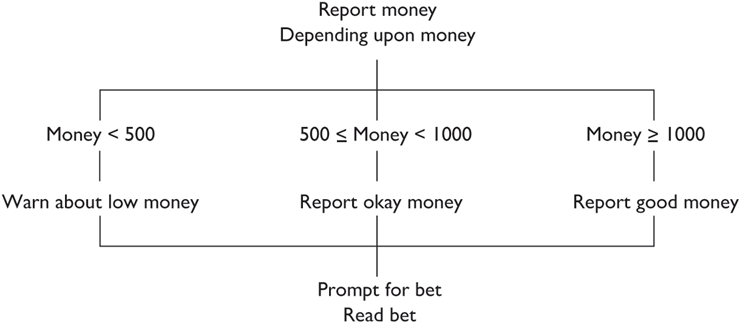
\includegraphics[width=\maxwidth,height=\maxheight,width=0.9\linewidth]{Figures/img_p247_1.png}
\end{center}

Do đó, đoạn mã trước có thể được rút gọn thành phiên bản súc tích hơn
sau:

\begin{verbatim}
System.out.println("You have $" + money + " left.");
if (money < 500) {
    System.out.print("Cash is dangerously low. Bet carefully.");
} else if (money < 1000) {
    System.out.print("Cash is somewhat low. Bet moderately.");
} else {
    System.out.print("Cash is in good shape. Bet liberally.");
}
System.out.print("How much do you want to bet? ");
bet = console.nextInt();
\end{verbatim}

\subsubsection{Kiểm tra nhiều điều kiện (Testing Multiple
Conditions)}\label{kiux1ec3m-tra-nhiux1ec1u-ux111iux1ec1u-kiux1ec7n-testing-multiple-conditions}

Khi bạn đang viết một chương trình, bạn thường thấy mình muốn kiểm tra
nhiều hơn một điều kiện. Ví dụ, giả sử bạn muốn chương trình thực hiện
một hành động cụ thể nếu một số nằm trong khoảng từ 1 đến 10. Bạn có thể
viết:

\begin{verbatim}
if (number >= 1) {
    if (number <= 10) {
        doSomething();
    }
}
\end{verbatim}

Trong những dòng mã này, bạn phải viết hai câu lệnh: một câu lệnh kiểm
tra xem số đó có lớn hơn hoặc bằng 1 hay không và một câu lệnh kiểm tra
xem số đó có nhỏ hơn hoặc bằng 10 hay không.

Java cung cấp một giải pháp thay thế hiệu quả: Bạn có thể kết hợp hai
bài kiểm tra bằng cách sử dụng một toán tử được gọi là toán tử logic AND
(logical AND operator), được viết bằng hai dấu và không có khoảng trắng
ở giữa (\texttt{\&\&}). Sử dụng toán tử AND, chúng ta có thể viết đoạn
mã trước đơn giản hơn:

\begin{verbatim}
if (number >= 1 && number <= 10) {
    doSomething();
}
\end{verbatim}

Đúng như tên gọi của nó, toán tử AND tạo thành một biểu thức kiểm tra
yêu cầu cả hai phần của biểu thức kiểm tra đều phải đánh giá thành
\texttt{true}. Có một toán tử tương tự được gọi là logic OR (logical OR)
đánh giá thành \texttt{true} nếu một trong hai biểu thức kiểm tra đánh
giá thành \texttt{true}. Toán tử logic OR được viết bằng cách sử dụng
hai ký tự gạch đứng (\texttt{\textbar{}\textbar{}}). Ví dụ, nếu bạn muốn
kiểm tra xem một biến \texttt{number} có bằng 1 hoặc 2 hay không, bạn có
thể viết:

\begin{verbatim}
if (number == 1 || number == 2) {
    processNumber(number);
}
\end{verbatim}

Chúng ta sẽ khám phá các toán tử logic AND và logic OR chi tiết hơn
trong chương tiếp theo.

\subsection{Các thuật toán tích lũy (Cumulative
Algorithms)}\label{cuxe1c-thuux1eadt-touxe1n-tuxedch-lux169y-cumulative-algorithms-1}

Bạn càng lập trình nhiều, bạn sẽ càng thấy rằng một số mẫu nhất định
xuất hiện. Nhiều thuật toán phổ biến liên quan đến việc tích lũy một câu
trả lời theo từng bước. Trong phần này, chúng ta sẽ khám phá một số
thuật toán tích lũy phổ biến nhất.

\begin{quote}
\textbf{Thuật toán tích lũy (Cumulative Algorithm)} Một thao tác trong
đó một giá trị tổng thể được tính toán tăng dần, thường sử dụng một vòng
lặp.
\end{quote}

Ví dụ, bạn có thể sử dụng một thuật toán tích lũy trên một tập hợp các
số để tính giá trị trung bình hoặc để tìm số lớn nhất.

\subsubsection{Tính tổng tích lũy (Cumulative
Sum)}\label{tuxednh-tux1ed5ng-tuxedch-lux169y-cumulative-sum}

Bạn sẽ thường muốn tìm tổng của một chuỗi các số. Một cách để làm điều
này là khai báo một biến khác nhau cho mỗi giá trị mà bạn muốn bao gồm,
nhưng đó sẽ không phải là một giải pháp thiết thực: Nếu bạn phải cộng

hàng trăm con số với nhau, bạn sẽ không muốn khai báo hàng trăm biến
khác nhau. May mắn thay, có một cách đơn giản hơn.

Thủ thuật là giữ một bảng kiểm đếm liên tục (running tally) của kết quả
và xử lý từng số một. Ví dụ, để cộng thêm vào một biến có tên là
\texttt{sum}, bạn sẽ viết dòng mã sau:

\begin{verbatim}
sum = sum + next;
\end{verbatim}

Ngoài ra, bạn có thể sử dụng toán tử gán viết tắt (shorthand assignment
operator):

\begin{verbatim}
sum += next;
\end{verbatim}

Câu lệnh trước đó lấy giá trị hiện tại của \texttt{sum}, cộng thêm giá
trị của một biến có tên là \texttt{next} và lưu trữ kết quả dưới dạng
giá trị mới của \texttt{sum}. Thao tác này được thực hiện cho mỗi số cần
tính tổng. Lưu ý rằng khi bạn thực thi câu lệnh này lần đầu tiên,
\texttt{sum} không có giá trị. Để giải quyết vấn đề này, bạn khởi tạo
\texttt{sum} bằng một giá trị sẽ không ảnh hưởng đến câu trả lời:
\texttt{0}.

Đây là một mô tả bằng mã giả của thuật toán tính tổng tích lũy:

\begin{verbatim}
sum = 0.
for (tất cả các số cần tính tổng) {
    lấy "next".
    sum += next.
}
\end{verbatim}

Để triển khai thuật toán này, bạn phải quyết định số lần thực hiện vòng
lặp và cách lấy giá trị \texttt{next}. Dưới đây là một chương trình
tương tác nhắc người dùng nhập số lượng các số cần cộng lại với nhau và
bản thân các số đó:

\begin{verbatim}
 1 // Finds the sum of a sequence of numbers.
 2
 3 import java.util.*;
 4
 5 public class ExamineNumbers1 {
 6     public static void main(String[] args) {
 7         System.out.println("This program adds a sequence of");
 8         System.out.println("numbers.");
 9         System.out.println();
10
11         Scanner console = new Scanner(System.in);
12
13         System.out.print("How many numbers do you have? ");
14         int totalNumber = console.nextInt();
15
16         double sum = 0.0;
17         for (int i = 1; i <= totalNumber; i++) {
18              System.out.print("    #" + i + "? ");
19              double next = console.nextDouble();
20             sum += next;
21         }
22         System.out.println();
23
24         System.out.println("sum = " + sum);
25     }
26 }
\end{verbatim}

Quá trình thực thi của chương trình sẽ trông giống như thế này (như
thường lệ, dữ liệu người dùng nhập được in đậm):

\begin{verbatim}
This program adds a sequence of 
numbers. 
How many numbers do you have? 6  
    #1? 3.2  
    #2? 4.7  
    #3? 5.1  
    #4? 9.0  
    #5? 2.4  
    #6? 3.1  
sum = 27.5
\end{verbatim}

Hãy theo dõi quá trình thực thi một cách chi tiết. Trước khi vào vòng
lặp \texttt{for}, chúng ta khởi tạo biến \texttt{sum} thành
\texttt{0.0}:

\begin{center}
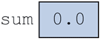
\includegraphics[width=\maxwidth,height=\maxheight,width=0.9\linewidth]{Figures/img_p254_0.png}
\end{center}

Ở lần thực thi đầu tiên của vòng lặp \texttt{for}, chúng ta đọc một giá
trị \texttt{3.2} từ người dùng và cộng giá trị này vào \texttt{sum}:

\begin{center}
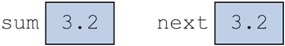
\includegraphics[width=\maxwidth,height=\maxheight,width=0.9\linewidth]{Figures/img_p254_1.png}
\end{center}

Lần thứ hai qua vòng lặp, chúng ta đọc một giá trị \texttt{4.7} và cộng
vào giá trị của \texttt{sum}:

\begin{center}
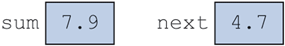
\includegraphics[width=\maxwidth,height=\maxheight,width=0.9\linewidth]{Figures/img_p254_2.png}
\end{center}

Lưu ý rằng \texttt{sum} hiện đã bao gồm cả hai số mà người dùng đã nhập,
vì chúng ta đã cộng giá trị mới, \texttt{4.7}, vào giá trị cũ,
\texttt{3.2}. Lần thứ ba qua vòng lặp, chúng ta cộng giá trị
\texttt{5.1}:

\begin{center}
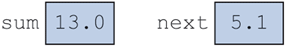
\includegraphics[width=\maxwidth,height=\maxheight,width=0.9\linewidth]{Figures/img_p254_3.png}
\end{center}

Lưu ý rằng biến \texttt{sum} hiện chứa tổng của ba số đầu tiên
(\texttt{3.2\ +\ 4.7\ +\ 5.1}). Bây giờ chúng ta đọc vào \texttt{9.0} và
cộng nó vào tổng:

\begin{center}
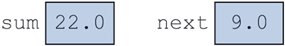
\includegraphics[width=\maxwidth,height=\maxheight,width=0.9\linewidth]{Figures/img_p255_0.png}
\end{center}

Sau đó, chúng ta cộng giá trị thứ năm, \texttt{2.4}:

\begin{center}
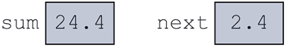
\includegraphics[width=\maxwidth,height=\maxheight,width=0.9\linewidth]{Figures/img_p255_1.png}
\end{center}

Cuối cùng, chúng ta cộng giá trị thứ sáu, \texttt{3.1}:

\begin{center}
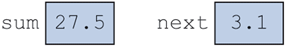
\includegraphics[width=\maxwidth,height=\maxheight,width=0.9\linewidth]{Figures/img_p255_2.png}
\end{center}

Sau đó, chúng ta thoát khỏi vòng lặp \texttt{for} và in ra giá trị của
\texttt{sum}.

Có một vấn đề phạm vi (scope) thú vị trong chương trình cụ thể này. Lưu
ý rằng biến \texttt{sum} được khai báo bên ngoài vòng lặp, trong khi
biến \texttt{next} được khai báo bên trong vòng lặp. Chúng ta không có
lựa chọn nào khác ngoài việc khai báo \texttt{sum} bên ngoài vòng lặp vì
nó cần được khởi tạo và nó được sử dụng sau vòng lặp. Nhưng biến
\texttt{next} chỉ được sử dụng bên trong vòng lặp, vì vậy nó có thể được
khai báo trong phạm vi bên trong đó. Tốt nhất là khai báo các biến trong
phạm vi trong cùng (innermost scope) có thể.

Thuật toán tính tổng tích lũy và các biến thể của nó sẽ hữu ích trong
nhiều tác vụ lập trình mà bạn giải quyết. Làm thế nào bạn có thể thực
hiện một phép tính tích tích lũy (cumulative product)? Đây là mã giả:

\begin{verbatim}
product = 1.
for (tất cả các số cần nhân) {
    lấy "next".
    product = product * next.
}
\end{verbatim}

\subsubsection{Vòng lặp tìm
Min/Max}\label{vuxf2ng-lux1eb7p-tuxecm-minmax}

Một tác vụ lập trình phổ biến khác là theo dõi các giá trị lớn nhất
và/hoặc nhỏ nhất trong một chuỗi. Ví dụ, hãy xem xét tác vụ quyết định
xem liệu có khả thi để xây dựng một khu vực sống trên Mặt trăng cho con
người ở hay không. Một trở ngại là nhiệt độ bề mặt trung bình hàng ngày
trên Mặt trăng là một mức lạnh giá -50 độ Fahrenheit. Nhưng một vấn đề
khó khăn hơn nhiều là phạm vi giá trị rộng; nó dao động từ mức tối thiểu
là -240 độ đến tối đa là 250 độ.

Để tính toán giá trị lớn nhất của một chuỗi các giá trị, bạn có thể theo
dõi giá trị lớn nhất mà bạn đã thấy cho đến nay và sử dụng lệnh
\texttt{if} để cập nhật giá trị lớn nhất nếu bạn bắt gặp một giá trị mới
lớn hơn giá trị lớn nhất hiện tại. Cách tiếp cận này có thể được mô tả
bằng mã giả như sau:

\begin{verbatim}
khởi tạo max.
for (tất cả các số cần kiểm tra) {
     lấy "next".
     if (next > max) {
        max = next.
    }
}
\end{verbatim}

Việc khởi tạo giá trị lớn nhất không hề đơn giản như bạn tưởng. Ví dụ,
những người mới học thường khởi tạo \texttt{max} thành \texttt{0}. Nhưng
chuyện gì sẽ xảy ra nếu chuỗi số mà bạn đang kiểm tra hoàn toàn bao gồm
các số âm? Ví dụ, bạn có thể được yêu cầu tìm giá trị lớn nhất của chuỗi
này:

-84, -7, -14, -39, -410, -17, -41, -9

Giá trị lớn nhất trong chuỗi này là -7 nhưng nếu bạn đã khởi tạo
\texttt{max} thành \texttt{0}, chương trình sẽ báo cáo không chính xác
\texttt{0} là giá trị lớn nhất.

Có hai giải pháp kinh điển cho vấn đề này. Đầu tiên, nếu bạn biết phạm
vi của các số bạn đang kiểm tra, bạn có thể đưa ra lựa chọn thích hợp
cho \texttt{max}. Trong trường hợp đó, bạn có thể đặt \texttt{max} thành
giá trị thấp nhất trong phạm vi. Điều đó có vẻ phản trực giác vì thông
thường chúng ta nghĩ giá trị lớn nhất là lớn, nhưng ý tưởng là đặt
\texttt{max} thành giá trị nhỏ nhất có thể để bất kỳ thứ gì lớn hơn sẽ
khiến \texttt{max} được đặt lại thành giá trị đó. Ví dụ, nếu bạn biết
rằng chuỗi nhiệt độ trước đó bao gồm các độ Fahrenheit, bạn sẽ biết rằng
nhiệt độ không bao giờ có thể nhỏ hơn độ không tuyệt đối (khoảng -460 độ
Fahrenheit), vì vậy bạn có thể khởi tạo \texttt{max} thành giá trị đó.

Khả năng thứ hai là khởi tạo \texttt{max} thành giá trị đầu tiên trong
chuỗi. Điều đó sẽ không phải lúc nào cũng thuận tiện vì nó có nghĩa là
phải lấy một trong các số bên ngoài vòng lặp.

Khi bạn kết hợp hai khả năng này, mã giả sẽ trở thành:

\begin{verbatim}
khởi tạo max bằng giá trị thấp nhất có thể hoặc bằng giá trị đầu tiên.
for (tất cả các số cần kiểm tra) {
    lấy "next".
    if (next > max) {
         max = next;
    }
}
\end{verbatim}

Mã giả để tính toán giá trị nhỏ nhất là một biến thể nhỏ của đoạn mã
này:

\begin{verbatim}
khởi tạo min bằng giá trị cao nhất có thể hoặc bằng giá trị đầu tiên.
for (tất cả các số cần kiểm tra) {
     lấy "next".
     if (next < min) {
         min = next.
    }
}
\end{verbatim}

Để giúp bạn hiểu rõ hơn về điều này, hãy đưa mã giả vào hành động với
một bài toán thực tế. Trong toán học, có một bài toán mở liên quan đến
những gì được gọi là dãy mưa đá (hailstone sequences). Các chuỗi số này
thường tăng và giảm theo các mô hình không thể đoán trước, hơi giống với
quá trình hình thành mưa đá. Một chuỗi mưa đá là một chuỗi các số trong
đó mỗi giá trị \(x\) được theo sau bởi:

\(3x + 1\), nếu \(x\) là số lẻ \(x / 2\), nếu \(x\) là số chẵn

Ví dụ, nếu bạn bắt đầu với 7 và tạo ra một chuỗi có độ dài 10, bạn sẽ
nhận được chuỗi: 7, 22, 11, 34, 17, 52, 26, 13, 40, 20 Trong chuỗi này,
giá trị lớn nhất và nhỏ nhất lần lượt là 52 và 7. Nếu bạn mở rộng phép
tính này cho một chuỗi có độ dài 20, bạn sẽ nhận được chuỗi: 7, 22, 11,
34, 17, 52, 26, 13, 40, 20, 10, 5, 16, 8, 4, 2, 1, 4, 2, 1 Trong trường
hợp này, giá trị lớn nhất và nhỏ nhất lần lượt là 52 và 1.

Bạn sẽ nhận thấy rằng một khi 1, 2, hoặc 4 xuất hiện trong chuỗi, chuỗi
sẽ tự lặp lại. Có giả thuyết cho rằng tất cả các số nguyên cuối cùng đều
đạt đến 1, giống như những hạt mưa đá rơi xuống đất. Đây là một bài toán
chưa có lời giải trong toán học. Không ai có thể bác bỏ nó, nhưng cũng
không ai chứng minh được nó.

Hãy viết một phương thức lấy một giá trị bắt đầu và độ dài chuỗi và in
ra giá trị lớn nhất và nhỏ nhất thu được trong một chuỗi mưa đá được tạo
bởi giá trị bắt đầu đó và có độ dài đó. Phương thức của chúng ta sẽ
trông như thế này:

\begin{verbatim}
public static void printHailstoneMaxMin(int value, int length) {
    ...
}
\end{verbatim}

Chúng ta có thể sử dụng giá trị bắt đầu để khởi tạo \texttt{max} và
\texttt{min}:

\begin{verbatim}
int min = value;
int max = value;
\end{verbatim}

Sau đó, chúng ta cần một vòng lặp sẽ tạo ra các giá trị khác. Lời gọi
phương thức sẽ cung cấp một giá trị cho tham số \texttt{length} cho
chúng ta biết số lần phải lặp qua vòng lặp, nhưng chúng ta không muốn
thực thi phần thân vòng lặp số lần bằng \texttt{length}: Hãy nhớ rằng
giá trị bắt đầu là một phần của chuỗi, vì vậy nếu chúng ta muốn sử dụng
một chuỗi có độ dài đã cho, chúng ta phải đảm bảo rằng số vòng lặp ít
hơn độ dài một đơn vị. Kết hợp ý tưởng này với mã giả
\texttt{max}/\texttt{min}, chúng ta biết vòng lặp sẽ trông như thế này:

\begin{verbatim}
for (int i = 1; i <= length - 1; i++) {
    tính số tiếp theo.
    if (value > max) {
         max = value.
    } else if (value < min) {
         min = value.
    }
}
in max và min.
\end{verbatim}

Để điền vào mã giả cho ``tính số tiếp theo'', chúng ta cần dịch công
thức toán học mưa đá sang mã. Công thức này khác nhau, tùy thuộc vào
việc giá trị hiện tại là lẻ hay chẵn. Chúng ta có thể sử dụng lệnh
\texttt{if/else} để giải quyết tác vụ này. Đối với biểu thức kiểm tra,
chúng ta có thể sử dụng phép kiểm tra ``mod 2'' để xem chúng ta nhận
được phần dư là bao nhiêu khi chia cho 2. Số chẵn có phần dư là 0 và số
lẻ có phần dư là 1. Vì vậy, biểu thức kiểm tra sẽ trông như thế này:

\begin{verbatim}
if (value % 2 == 0) {
    thực hiện phép tính chẵn.
} else {
    thực hiện phép tính lẻ.
}
\end{verbatim}

Dịch các công thức toán học mưa đá sang Java, chúng ta nhận được đoạn mã
sau:

\begin{verbatim}
if (value % 2 == 0) {
    value = value / 2;
} else {
    value = 3 * value + 1;
}
\end{verbatim}

Phần duy nhất trong mã giả của chúng ta mà chúng ta chưa điền là phần in
ra kết quả. Phần này diễn ra sau vòng lặp và khá dễ hoàn thành. Đây là
phương thức hoàn chỉnh:

\begin{verbatim}
public static void printHailstoneMaxMin(int value, int length) {
    int min = value;
    int max = value;
  for (int i = 1; i <= length - 1; i++) {
      if (value % 2 == 0) {
          value = value / 2;
      } else {
          value = 3 * value + 1;
      }
      if (value > max) {
          max = value;
      } else if (value < min) {
          min = value;
      }
  }
  System.out.println("max = " + max);
  System.out.println("min = " + min);
}
\end{verbatim}

\subsubsection{Tính tổng tích lũy với
if}\label{tuxednh-tux1ed5ng-tuxedch-lux169y-vux1edbi-if}

Bây giờ chúng ta hãy khám phá cách bạn có thể sử dụng các lệnh
\texttt{if/else} để tạo ra một số biến thể thú vị trên thuật toán tính
tổng tích lũy.

Giả sử bạn muốn đọc một chuỗi số và tính trung bình. Tác vụ này có vẻ
giống như một biến thể đơn giản của mã tính tổng tích lũy. Bạn có thể
tính trung bình bằng tổng chia cho số lượng số:

\begin{verbatim}
double average = sum / totalNumber;
System.out.println("average = " + average);
\end{verbatim}

Nhưng có một vấn đề nhỏ với đoạn mã này. Giả sử rằng khi chương trình
hỏi người dùng số lượng số cần xử lý, người dùng nhập \texttt{0}. Sau đó
chương trình sẽ không vào vòng lặp tính tổng tích lũy và mã của bạn sẽ
cố gắng tính giá trị của \texttt{0} chia cho \texttt{0}. Java sau đó sẽ
in ra trung bình là \texttt{NaN}, một thông báo khó hiểu viết tắt của
``Not a Number''. Sẽ tốt hơn nếu chương trình in ra một loại thông báo
khác cho biết không có số nào để tính trung bình. Bạn có thể sử dụng một
lệnh \texttt{if/else} cho mục đích này:

\begin{verbatim}
if (totalNumber <= 0) {
    System.out.println("No numbers to average");
} else {
    double average = sum / totalNumber;
    System.out.println("average = " + average);
}
\end{verbatim}

Một cách sử dụng khác của lệnh \texttt{if} sẽ là đếm số lượng số âm mà
người dùng nhập vào. Bạn sẽ thường muốn đếm số lần một điều gì đó xảy ra
trong chương trình. Mục tiêu này dễ dàng đạt được với một lệnh
\texttt{if} và một biến số nguyên được gọi là bộ đếm (counter). Bạn bắt
đầu bằng cách khởi tạo bộ đếm thành \texttt{0}:

\begin{verbatim}
int negatives = 0;
\end{verbatim}

Bạn có thể sử dụng bất kỳ tên nào bạn muốn cho biến. Ở đây chúng tôi sử
dụng \texttt{negatives} bởi vì đó là những gì bạn đang đếm. Bước cần
thiết khác là tăng bộ đếm bên trong vòng lặp nếu nó vượt qua bài kiểm
tra đang được quan tâm:

\begin{verbatim}
if (next < 0) {
    negatives++;
}
\end{verbatim}

Khi bạn kết hợp tất cả những điều này lại với nhau và sửa đổi các chú
thích cũng như phần giới thiệu, bạn sẽ có biến thể sau của chương trình
tính tổng tích lũy:

\begin{verbatim}
 1 // Finds the average of a sequence of numbers as well as
 2 // reporting how many of the user-specified numbers were negative.
 3
 4 import java.util.*;
 5
 6 public class ExamineNumbers2 {
 7     public static void main(String[] args) {
 8         System.out.println("This program examines a sequence");
 9         System.out.println("of numbers to find the average");
10         System.out.println("and count how many are negative.");
\end{verbatim}

\begin{verbatim}
           negatives++;
        }
    }
    System.out.println();

    if (totalNumber <= 0) {
       System.out.println("No numbers to average");
   } else {
       double average = sum / totalNumber;
       System.out.println("average = " + average);
   }
   System.out.println("# of negatives = " + negatives);
 }
}
\end{verbatim}

Quá trình thực thi của chương trình sẽ trông giống như thế này:

\begin{verbatim}
This program examines a sequence 
of numbers to find the average 
and count how many are negative. 
 
How many numbers do you have? 8  
    #1? 2.5  
    #2? 9.2  
    #3? -19.4  
    #4? 208.2  
    #5? 42.3  
    #6? 92.7  
    #7? -17.4  
    #8? 8  
average = 40.7625 
# of negatives = 2
\end{verbatim}

\subsubsection{Sai số làm tròn (Roundoff
Errors)}\label{sai-sux1ed1-luxe0m-truxf2n-roundoff-errors}

Khi bạn khám phá các thuật toán tích lũy, bạn sẽ phát hiện ra một vấn đề
cụ thể mà bạn nên hiểu. Ví dụ, hãy xem xét lần thực thi sau của chương
trình \texttt{ExamineNumbers2} trước đó với dữ liệu đầu vào khác của
người dùng:

\begin{verbatim}
This program examines a sequence 
of numbers to find the average 
and count how many are negative. 
 
How many numbers do you have? 4 
    #1? 2.1  
    #2? -3.8  
    #3? 5.4  
    #4? 7.4  
average = 2.7750000000000004 
# of negatives = 1
\end{verbatim}

Nếu bạn sử dụng máy tính, bạn sẽ thấy rằng bốn số cộng lại bằng 11.1.
Nếu bạn chia số này cho 4, bạn sẽ nhận được 2.775. Tuy nhiên, Java báo
cáo kết quả là \texttt{2.7750000000000004}. Tất cả những số 0 đó từ đâu
ra và tại sao số đó lại kết thúc bằng số 4? Câu trả lời là các số dấu
phẩy động (floating-point numbers) có thể dẫn đến sai số làm tròn
(roundoff errors).

\begin{quote}
\textbf{Sai số làm tròn (Roundoff Error)} Lỗi số học xảy ra do các số
dấu phẩy động được lưu trữ dưới dạng giá trị gần đúng chứ không phải là
giá trị chính xác.
\end{quote}

Các sai số làm tròn nhìn chung là nhỏ và có thể xảy ra theo một trong
hai hướng (hơi cao hoặc hơi thấp). Trong trường hợp trước, chúng ta gặp
sai số làm tròn hơi cao.

Các số dấu phẩy động được lưu trữ ở định dạng tương tự như ký hiệu khoa
học (scientific notation), với một tập hợp các chữ số và một số mũ
(exponent). Hãy xem xét cách bạn sẽ lưu trữ giá trị một phần ba bằng ký
hiệu khoa học ở cơ số 10. Bạn sẽ nói rằng số đó là 3.33333 (lặp lại)
nhân với 10 lũy thừa -1. Tuy nhiên, chúng ta không thể lưu trữ vô số chữ
số trên máy tính, vì vậy chúng ta sẽ phải ngừng lặp lại số 3 ở một thời
điểm nào đó. Giả sử chúng ta có thể lưu trữ 10 chữ số. Khi đó, giá trị
của một phần ba sẽ được lưu trữ là 3.333333333 nhân với 10 lũy thừa -1.
Nếu chúng ta nhân số đó với 3, chúng ta không nhận lại được 1. Thay vào
đó, chúng ta nhận được 9.999999999 nhân với 10 lũy thừa -1 (tương đương
với 0.9999999999).

Bạn có thể thắc mắc tại sao các số chúng ta sử dụng trong ví dụ trước
lại gây ra sự cố khi chúng không có bất kỳ chữ số lặp lại nào. Bạn phải
nhớ rằng máy tính lưu trữ các số ở cơ số 2. Các số như 2.1 và 5.4 có thể
trông giống như các số đơn giản ở cơ số 10, nhưng chúng có các chữ số
lặp lại khi được lưu trữ ở cơ số 2.

Sai số làm tròn có thể dẫn đến những kết quả khá bất ngờ. Ví dụ, hãy xem
xét chương trình ngắn sau đây:

\begin{verbatim}
 1 // This program demonstrates roundoff errors.
 2 public class Roundoff {
 3     public static void main(String[] args) {
 4         double n = 1.0;
 5         for (int i = 1; i <= 10; i++) {
 6              n += 0.1;
 7             System.out.println(n);
 8         }
 9     }
10 }
\end{verbatim}

Chương trình này trình bày một phép tính tổng tích lũy cổ điển với một
vòng lặp cộng thêm \texttt{0.1} vào biến \texttt{n} mỗi lần vòng lặp
thực thi. Chúng ta bắt đầu với \texttt{n} bằng \texttt{1.0} và vòng lặp
lặp lại 10 lần, điều mà chúng ta có thể mong đợi sẽ in ra các số 1.1,
1.2, 1.3 và vân vân cho đến 2.0. Thay vào đó, nó tạo ra kết quả sau:

\begin{verbatim}
1.1 
\end{verbatim}

\begin{verbatim}
1.2000000000000002 
1.3000000000000003 
1.4000000000000004 
1.5000000000000004 
1.6000000000000005 
1.7000000000000006 
1.8000000000000007 
1.9000000000000008 
2.000000000000001
\end{verbatim}

Vấn đề xảy ra vì 0.1 không thể được lưu trữ chính xác ở cơ số 2 (nó tạo
ra một tập hợp các chữ số lặp lại, giống như một phần ba ở cơ số 10).
Mỗi lần lặp qua vòng lặp, lỗi lại được cộng dồn, đó là lý do tại sao sai
số làm tròn lại trở nên tồi tệ hơn sau mỗi lần lặp.

Như một ví dụ khác, hãy xem xét tác vụ cộng các giá trị của một đồng xu
một xu, một đồng 5 xu, một đồng 10 xu và một đồng 25 xu. Nếu chúng ta sử
dụng các biến kiểu \texttt{int}, chúng ta sẽ nhận được câu trả lời chính
xác bất kể thứ tự mà chúng ta cộng các số:

\begin{verbatim}
jshell> int cents1 = 1 + 5 + 10 + 25; 
cents1 ==> 41
jshell> int cents2 = 25 + 10 + 5 + 1; 
cents2 ==> 41
\end{verbatim}

Bất kể thứ tự như thế nào, các con số này luôn cộng lại bằng 41 xu.
Nhưng giả sử thay vì nghĩ về các giá trị này là toàn bộ số xu, chúng ta
nghĩ về chúng như một phần nhỏ của đồng đô la mà chúng ta lưu trữ dưới
dạng \texttt{double}:

\begin{verbatim}
jshell> double dollars1 = 0.01 + 0.05 + 0.10 + 0.25; 
dollars1 ==> 0.41000000000000003
jshell> double dollars2 = 0.25 + 0.10 + 0.05 + 0.01; 
dollars2 ==> 0.41
\end{verbatim}

Mặc dù chúng ta cộng chính xác cùng những con số, thực tế là chúng ta
cộng chúng theo một thứ tự khác lại tạo ra sự khác biệt. Lý do là sai số
làm tròn.

Có một số bài học cần rút ra từ điều này: - Hãy nhận biết rằng khi bạn
lưu trữ các giá trị dấu phẩy động (ví dụ: \texttt{double}), bạn đang lưu
trữ các giá trị gần đúng chứ không phải là các giá trị chính xác. Nếu
bạn cần lưu trữ một giá trị chính xác, hãy lưu trữ nó bằng kiểu
\texttt{int}. - Đừng ngạc nhiên khi bạn thấy các con số hơi khác so với
các giá trị dự kiến. - Đừng mong đợi có thể so sánh các biến kiểu
\texttt{double} để kiểm tra sự bằng nhau.

Để theo dõi ý thứ ba, hãy xem xét đoạn mã trước đó sẽ dẫn đến điều gì
nếu chúng ta thực hiện biểu thức kiểm tra sau:

\begin{verbatim}
if (dollars1 == dollars2) {
   ...
}
\end{verbatim}

Biểu thức kiểm tra sẽ đánh giá thành \texttt{false} bởi vì các giá trị
rất gần nhau, nhưng không đủ gần để Java coi chúng là bằng nhau. Chúng
ta hiếm khi sử dụng bài kiểm tra về sự bằng nhau chính xác khi làm việc
với \texttt{double}. Thay vào đó, chúng ta có thể sử dụng một biểu thức
kiểm tra như thế này để xem liệu các số có gần bằng nhau không:

\begin{verbatim}
if (Math.abs(dollars1 - dollars2) < 0.001) {
   ...
}
\end{verbatim}

Chúng ta sử dụng phương thức giá trị tuyệt đối (\texttt{abs}) từ lớp
\texttt{Math} để tìm độ lớn của phần chênh lệch và sau đó kiểm tra xem
nó có nhỏ hơn một lượng nhỏ nào đó không (trong trường hợp này là
\texttt{0.001}).

Phần sau trong chương này, chúng tôi sẽ giới thiệu một biến thể của
\texttt{print}/\texttt{println} được gọi là \texttt{printf} sẽ giúp việc
in các số như thế này mà không có tất cả các chữ số thừa dễ dàng hơn.

\subsection{Xử lý văn bản (Text
Processing)}\label{xux1eed-luxfd-vux103n-bux1ea3n-text-processing-1}

Các lập trình viên thường phải đối mặt với các bài toán yêu cầu họ phải
tạo, chỉnh sửa, kiểm tra và định dạng văn bản. Nói chung, chúng tôi gọi
những tác vụ này là xử lý văn bản.

\begin{quote}
\textbf{Xử lý văn bản (Text Processing)} Chỉnh sửa và định dạng chuỗi
văn bản.
\end{quote}

Trong phần này, chúng ta sẽ xem xét chi tiết hơn về kiểu dữ liệu nguyên
thủy \texttt{char} và giới thiệu một lệnh mới được gọi là
\texttt{System.out.printf}. Cả hai công cụ này đều rất hữu ích cho các
tác vụ xử lý văn bản.

\subsubsection{Kiểu char}\label{kiux1ec3u-char}

Kiểu dữ liệu nguyên thủy \texttt{char} đại diện cho một ký tự văn bản
duy nhất. Việc có các biến, tham số và giá trị trả về có kiểu
\texttt{char} là hoàn toàn hợp lệ nếu bạn muốn. Các giá trị nghĩa đen
(literal values) của kiểu \texttt{char} được biểu thị bằng cách đặt ký
tự bên trong dấu nháy đơn:

\begin{verbatim}
char ch = 'A';
\end{verbatim}

Bạn cũng có thể tạo giá trị \texttt{char} đại diện cho một chuỗi thoát
(escape sequence):

\begin{verbatim}
char newline = '\n';
\end{verbatim}

Trong chương trước, chúng ta đã thảo luận về các đối tượng
\texttt{String}. Sự khác biệt giữa \texttt{char} và \texttt{String} là
một sự khác biệt tinh tế khiến nhiều lập trình viên Java mới bối rối. Sự
khác biệt chính là \texttt{String} là một đối tượng, nhưng \texttt{char}
là một giá trị nguyên thủy. Một \texttt{char} chiếm một dung lượng bộ
nhớ rất nhỏ, nhưng nó không có các phương thức. Bảng 4.4 tóm tắt một số
khác biệt giữa các kiểu.

Bảng 4.4 Sự khác biệt giữa \texttt{char} và \texttt{String}

\begin{center}

\includegraphics[width=\maxwidth,height=\maxheight,width=0.9\linewidth]{Figures/img_p275_0.png}
\end{center}

Tại sao Java lại có hai kiểu cho dữ liệu tương tự như vậy? Kiểu
\texttt{char} tồn tại chủ yếu vì những lý do lịch sử; nó có từ các ngôn
ngữ cũ hơn như C, ngôn ngữ đã ảnh hưởng đến thiết kế của Java.

Vậy tại sao một người lại sử dụng kiểu \texttt{char} khi \texttt{String}
có sẵn? Việc sử dụng \texttt{char} thường là cần thiết vì một số phương
thức trong API của Java sử dụng nó làm kiểu tham số hoặc kiểu trả về.
Nhưng cũng có

một vài trường hợp mà việc sử dụng \texttt{char} có thể hữu ích hoặc đơn
giản hơn việc sử dụng \texttt{String}.

Các ký tự của một \texttt{String} được lưu trữ bên trong đối tượng dưới
dạng các giá trị kiểu \texttt{char}. Bạn có thể truy cập các ký tự riêng
lẻ thông qua phương thức \texttt{charAt} của đối tượng, phương thức này
nhận một chỉ số nguyên làm tham số và trả về ký tự tại chỉ số đó. Chúng
ta thường lặp qua một chuỗi để kiểm tra hoặc thay đổi các ký tự của nó.
Ví dụ, phương thức sau in mỗi ký tự của một chuỗi trên một dòng riêng
của nó:

\begin{verbatim}
public static void printVertical(String message) {
    for (int i = 0; i < message.length(); i++) {
        char ch = message.charAt(i);
        System.out.println(ch);
    }
}
\end{verbatim}

\subsubsection{\texorpdfstring{\texttt{char} so với
\texttt{int}}{char so với int}}\label{char-so-vux1edbi-int}

Các giá trị kiểu \texttt{char} được lưu trữ nội bộ dưới dạng các số
nguyên. Một sơ đồ mã hóa tiêu chuẩn được gọi là Unicode xác định giá trị
số nguyên nào đại diện cho mỗi ký tự. (Unicode sẽ được đề cập chi tiết
hơn ở phần sau của chương này.) Vì các ký tự thực chất là các số nguyên,
Java sẽ tự động chuyển đổi giá trị kiểu \texttt{char} thành \texttt{int}
bất cứ khi nào nó mong đợi một \texttt{int}:

\begin{verbatim}
int letter = 'a' + 2; // stores 99
\end{verbatim}

Hóa ra giá trị số nguyên của
\texttt{\textquotesingle{}a\textquotesingle{}} là \texttt{97}, vì vậy
kết quả của biểu thức là \texttt{99}, được lưu trữ dưới dạng ký tự
\texttt{\textquotesingle{}c\textquotesingle{}}. Tương tự, một
\texttt{int} có thể được chuyển đổi thành một \texttt{char} bằng cách sử
dụng ép kiểu (type cast). (Việc ép kiểu là cần thiết như một lời hứa với
trình biên dịch, vì không phải mọi giá trị \texttt{int} có thể đều tương
ứng với một ký tự hợp lệ.) Dưới đây là ví dụ về một đoạn mã sử dụng ép
kiểu để chuyển đổi giá trị \texttt{int} thành giá trị kiểu
\texttt{char}:

\begin{verbatim}
int code = 66;
char grade = (char) code; // stores 'B'
\end{verbatim}

Vì các giá trị kiểu \texttt{char} thực chất là các số nguyên, chúng cũng
có thể được so sánh bằng các toán tử quan hệ như \texttt{\textless{}}
hoặc \texttt{==}. Ngoài ra, chúng có thể được sử dụng trong các vòng lặp
để bao phủ các phạm vi chữ cái. Ví dụ, đoạn mã sau in ra mọi chữ cái của
bảng chữ cái:

\begin{verbatim}
for (char letter = 'a'; letter <= 'z'; letter++) {
    System.out.print(letter);
}
\end{verbatim}

\begin{verbatim}
if (grade == 'B') {... // true
\end{verbatim}

Bạn có thể tìm hiểu thêm về sự tương đương giữa ký tự và số nguyên bằng
cách tìm kiếm trên web các bảng Unicode.

\subsubsection{Các thuật toán văn bản tích lũy (Cumulative Text
Algorithms)}\label{cuxe1c-thuux1eadt-touxe1n-vux103n-bux1ea3n-tuxedch-lux169y-cumulative-text-algorithms}

Các chuỗi ký tự thường được sử dụng trong các thuật toán tích lũy như đã
thảo luận ở phần trước trong chương này. Ví dụ, bạn có thể lặp qua các
ký tự của một chuỗi để tìm kiếm một chữ cái cụ thể. Phương thức sau chấp
nhận một chuỗi và một ký tự và trả về số lần ký tự đó xuất hiện trong
chuỗi:

\begin{verbatim}
public static int count(String text, char c) {
    int found = 0;
    for (int i = 0; i < text.length(); i++) {
        if (text.charAt(i) == c) {
            found++;
        }
    }
    return found;
}
\end{verbatim}

Một \texttt{char} có thể được ghép với một \texttt{String} bằng cách sử
dụng toán tử \texttt{+} tiêu chuẩn. Sử dụng ý tưởng này, một
\texttt{String} có thể được xây dựng bằng một vòng lặp, bắt đầu với một
chuỗi rỗng và ghép các ký tự riêng lẻ trong vòng lặp. Đây được gọi là
phép nối tích lũy (cumulative concatenation). Phương thức sau chấp nhận
một chuỗi và trả về các ký tự tương tự theo thứ tự ngược lại:

\begin{verbatim}
public static String reverse(String phrase) {
    String result = "";
    for (int i = 0; i < phrase.length(); i++) {
         result = phrase.charAt(i) + result;
    }
    return result;
}
\end{verbatim}

Ví dụ, lệnh gọi \texttt{reverse("Tin\ man\ ")} trả về
\texttt{"nam\ niT"}.

Vì \texttt{char} là một kiểu dữ liệu nguyên thủy, bạn không thể sử dụng
cú pháp dấu chấm để gọi các phương thức như cách bạn làm với một giá trị
kiểu \texttt{String}. Thay vào đó, Java cung cấp một lớp gọi là
\texttt{Character} có một số phương thức tĩnh (static methods) cho phép
bạn xác minh xem bạn có loại ký tự nào (chữ số, chữ cái, v.v.) và thực
hiện nhiều chuyển đổi khác nhau. Một số phương thức \texttt{Character}
hữu ích nhất được liệt kê trong Bảng 4.5.

Bảng 4.5 Các phương thức hữu ích của lớp \texttt{Character}

\begin{center}

\includegraphics[width=\maxwidth,height=\maxheight,width=0.9\linewidth]{Figures/img_p279_0.png}
\end{center}

Phương thức sau đếm số lượng chữ cái trong một \texttt{String}, bỏ qua
tất cả các ký tự không phải chữ cái như dấu câu, số và khoảng trắng:

\begin{verbatim}
public static int countLetters(String phrase) {
    int count = 0;
    for (int i = 0; i < phrase.length(); i++) {
        char ch = phrase.charAt(i);
          if (Character.isLetter(ch)) {
              count++;
        }
    }
    return count;
}
\end{verbatim}

Ví dụ, lệnh gọi \texttt{countLetters("gr8\ JoB!\ ")} trả về 5.

\subsubsection{System.out.printf}\label{system.out.printf}

Cho đến nay, chúng ta đã sử dụng \texttt{System.out.println} và
\texttt{System.out.print} cho đầu ra của bảng điều khiển (console
output). Có một phương thức thứ ba, \texttt{System.out.printf}, phức tạp
hơn một chút so với các phương thức khác nhưng cung cấp cho chúng ta một
số khả năng mới hữu ích. Chữ ``f'' trong \texttt{printf} là viết tắt của
``formatted'', ngụ ý rằng \texttt{System.out.printf} cung cấp cho bạn
nhiều quyền kiểm soát hơn đối với định dạng mà đầu ra của bạn được in
ra.

Hãy tưởng tượng rằng bạn muốn in một bảng cửu chương từ 1 đến 10. Đoạn
mã sau in ra các số chính xác, nhưng nó trông không được đẹp cho lắm:

\begin{verbatim}
for (int i = 1; i <= 10; i++) {
    for (int j = 1; j <= 10; j++) {
        System.out.print(i * j + " ");
    }
    System.out.println();
}
\end{verbatim}

Đầu ra là như sau. Lưu ý rằng các số không thẳng hàng theo chiều dọc:

\begin{verbatim}
1 2 3 4 5 6 7 8 9 10 
2 4 6 8 10 12 14 16 18 20 
3 6 9 12 15 18 21 24 27 30 
4 8 12 16 20 24 28 32 36 40 
5 10 15 20 25 30 35 40 45 50 
6 12 18 24 30 36 42 48 54 60 
7 14 21 28 35 42 49 56 63 70 
8 16 24 32 40 48 56 64 72 80 
9 18 27 36 45 54 63 72 81 90 
10 20 30 40 50 60 70 80 90 100
\end{verbatim}

Chúng ta có thể phân tách các số bằng các tab, điều này sẽ tốt hơn.
Nhưng sự phân tách này không cho chúng ta nhiều quyền kiểm soát đối với
giao diện của bảng. Mỗi số sẽ cách nhau chính xác tám khoảng trắng trên
màn hình và các số sẽ xuất hiện căn trái. Sẽ rất phiền phức nếu cố gắng
căn phải các số một cách thủ công, bởi vì bạn sẽ phải sử dụng các lệnh
\texttt{if/else} để kiểm tra xem một số cụ thể có nằm trong một phạm vi
nhất định hay không và, nếu cần, đệm nó với một số lượng khoảng trắng
nhất định.

\begin{quote}
\textbf{BẠN CÓ BIẾT?} \textbf{ASCII và Unicode} Chúng ta lưu trữ dữ liệu
trên máy tính dưới dạng số nhị phân (các chuỗi số 0 và 1). Để lưu trữ dữ
liệu văn bản, chúng ta cần một sơ đồ mã hóa cho chúng ta biết nên sử
dụng chuỗi số 0 và 1 nào cho bất kỳ ký tự nhất định nào. Hãy coi nó như
một chiếc nhẫn giải mã bí mật khổng lồ cho biết những điều như, ``Nếu
bạn muốn lưu trữ một chữ `a' thường, hãy sử dụng chuỗi 01100001.'' Đầu
những năm 1960, IBM đã phát triển một sơ đồ mã hóa gọi là EBCDIC hoạt
động tốt với các thẻ đục lỗ của công ty, thứ đã được sử dụng trong nhiều
thập kỷ trước khi máy tính được phát minh. Nhưng chẳng bao lâu sau, rõ
ràng EBCDIC không phải là một sơ đồ mã hóa thuận tiện cho các lập trình
viên máy tính. Có những khoảng trống trong chuỗi làm cho các ký tự như
`i' và `j' xuất hiện cách xa nhau mặc dù chúng đứng ngay sau nhau. Năm
1967, Hiệp hội Tiêu chuẩn Hoa Kỳ (American Standards Association) đã
công bố một sơ đồ được gọi là ASCII (phát âm là ``AS-kee'') được sử dụng
phổ biến kể từ đó. Tên viết tắt này là viết tắt của ``American Standard
Code for Information Interchange'' (Mã chuẩn Hoa Kỳ về trao đổi thông
tin). Ở dạng ban đầu, ASCII định nghĩa 128 ký tự, mỗi ký tự có thể được
lưu trữ với 7 bit dữ liệu. Vấn đề lớn nhất với ASCII là nó là một mã của
Mỹ. Có rất nhiều ký tự được sử dụng phổ biến ở các quốc gia khác không
được bao gồm trong ASCII. Ví dụ, đồng bảng Anh (£) và biến thể tiếng Tây
Ban Nha của chữ n (ñ) không được bao gồm trong 128 ký tự ASCII tiêu
chuẩn. Đã có nhiều nỗ lực nhằm mở rộng ASCII, nhân đôi nó lên 256 ký tự
để nó có thể bao gồm nhiều ký tự đặc biệt này. Tuy nhiên, hóa ra ngay cả
256 ký tự cũng không đủ để nắm bắt sự đa dạng đáng kinh ngạc của giao
tiếp của con người. Khoảng thời gian Java được tạo ra, một liên minh của
các chuyên gia phần mềm đã giới thiệu một tiêu chuẩn mới để mã hóa các
ký tự được gọi là Unicode. Họ quyết định rằng 7 bit của ASCII tiêu chuẩn
và 8 bit của ASCII mở rộng đơn giản là không đủ lớn và quyết định không
đặt giới hạn về số lượng bit họ có thể sử dụng để mã hóa ký tự. Tại thời
điểm viết bài này, liên minh đã xác định được hơn 110,000 ký tự, yêu cầu
nhiều hơn 16 bit một chút để lưu trữ. Unicode bao gồm các ký tự được sử
dụng trong hầu hết các ngôn ngữ hiện đại và thậm chí cả một số ngôn ngữ
cổ đại. Chữ tượng hình Ai Cập đã được thêm vào năm 2007, mặc dù nó vẫn
không bao gồm chữ tượng hình của người Maya và liên minh đã từ chối một
đề xuất bao gồm các ký tự Klingon. Các nhà thiết kế của Java đã sử dụng
Unicode làm tiêu chuẩn cho kiểu \texttt{char}, điều đó có nghĩa là các
chương trình Java có khả năng thao tác với đầy đủ các ký tự. May mắn
thay, Liên minh Unicode đã quyết định kết hợp các bảng mã ASCII, vì vậy
ASCII có thể được xem như một tập con của Unicode. Nếu bạn tò mò về thứ
tự thực tế của các ký tự trong ASCII, hãy gõ ``bảng ASCII'' vào công cụ
tìm kiếm yêu thích của bạn và bạn sẽ tìm thấy hàng triệu lượt truy cập
để khám phá.
\end{quote}

Một cách dễ dàng hơn nhiều để in các giá trị được căn lề trong các
trường có độ rộng cố định là sử dụng lệnh \texttt{System.out.printf}.
Phương thức \texttt{printf} chấp nhận một \texttt{String} được viết đặc
biệt gọi là chuỗi định dạng (format string) chỉ định giao diện chung của
đầu ra, theo sau là bất kỳ tham số nào sẽ được bao gồm trong đầu ra:

\begin{verbatim}
System.out.printf(<format string>, <parameter>,..., <parameter>);
\end{verbatim}

Một chuỗi định dạng giống như một \texttt{String} bình thường, ngoại trừ
việc nó có thể chứa các chỗ dành sẵn (placeholders) được gọi là công cụ
xác định định dạng (format specifiers) cho phép bạn chỉ định một vị trí
mà giá trị của một biến sẽ được chèn vào, cùng với định dạng bạn muốn
cung cấp cho giá trị đó. Các công cụ xác định định dạng bắt đầu bằng dấu
\texttt{\%} và kết thúc bằng một chữ cái xác định loại giá trị, chẳng
hạn như \texttt{d} cho số nguyên thập phân (\texttt{int}) hoặc
\texttt{f} cho số dấu phẩy động (số thực kiểu \texttt{double}). Hãy xem
xét lệnh \texttt{printf} sau:

\begin{verbatim}
int x = 38, y = -152;
System.out.printf("location: (%d, %d)\n", x, y);
\end{verbatim}

Lệnh này tạo ra đầu ra sau:

\begin{verbatim}
location: (38, -152)
\end{verbatim}

Dấu \texttt{\%d} không thực sự được in ra mà thay vào đó được thay thế
bằng tham số tương ứng được viết sau chuỗi định dạng. Số lượng công cụ
xác định định dạng trong chuỗi định dạng phải khớp với số lượng tham số
theo sau nó. Công cụ xác định đầu tiên sẽ được thay thế bằng tham số đầu
tiên, công cụ xác định thứ hai bằng tham số thứ hai, và vân vân.
\texttt{System.out.printf} là bất thường vì nó có thể chấp nhận một số
lượng tham số thay đổi.

Lệnh \texttt{printf} giống như \texttt{System.out.print} ở chỗ nó không
di chuyển sang một dòng mới trừ khi bạn ra lệnh rõ ràng cho nó làm như
vậy. Lưu ý rằng trong đoạn mã trước, chúng ta đã kết thúc chuỗi định
dạng của mình bằng \texttt{\textbackslash{}n} để hoàn thành dòng đầu ra.

Vì một công cụ xác định định dạng sử dụng \texttt{\%} làm ký tự đặc
biệt, nếu bạn muốn in ký hiệu \texttt{\%} thực tế trong một lệnh
\texttt{printf}, thay vào đó hãy viết hai ký tự \texttt{\%} liên tiếp.
Ví dụ:

\begin{verbatim}
int score = 87;
System.out.printf("You got %d%% on the exam!\n", score);
\end{verbatim}

Mã tạo ra đầu ra sau:

\begin{verbatim}
You got 87% on the exam!
\end{verbatim}

Một công cụ xác định định dạng có thể chứa thông tin sau dấu \texttt{\%}
để chỉ định chiều rộng, độ chính xác và căn lề của giá trị đang được in.
Ví dụ, \texttt{\%8d} chỉ định một số nguyên căn phải trong một khu vực
rộng 8 khoảng trắng và \texttt{\%12.4f} chỉ định một giá trị
\texttt{double} căn phải trong một khu vực rộng 12 khoảng trắng, được
làm tròn đến bốn chữ số sau dấu thập phân. Bảng 4.6 liệt kê một số công
cụ xác định định dạng phổ biến mà bạn có thể muốn sử dụng trong các
chương trình của mình.

Bảng 4.6 Các công cụ xác định định dạng phổ biến

\begin{center}

\includegraphics[width=\maxwidth,height=\maxheight,width=0.9\linewidth]{Figures/img_p286_0.png}
\end{center}

Như một ví dụ toàn diện, giả sử rằng các biến sau đã được khai báo để
biểu thị thông tin về một học sinh:

\begin{verbatim}
int score = 87;
double gpa = 3.18652;
String name = "Jessica";
\end{verbatim}

Đoạn mã mẫu sau in các biến trước đó bằng một số công cụ xác định định
dạng:

\begin{verbatim}
System.out.printf("student name: %10s\n", name);
System.out.printf("exam score  : %10d\n", score);
System.out.printf("GPA       : %10.2f\n", gpa);
\end{verbatim}

Mã tạo ra đầu ra sau:

\begin{verbatim}
student name:     Jessica 
exam score  :          87 
GPA       :        3.19
\end{verbatim}

Ba giá trị thẳng hàng ở cạnh phải của chúng, bởi vì chúng ta in tất cả
chúng với chiều rộng bằng 10. Phương thức \texttt{printf} giúp việc sắp
xếp các giá trị thành các cột theo cách này trở nên dễ dàng. Lưu ý rằng
điểm trung bình (GPA) của học sinh làm tròn thành 3.19, do số \texttt{2}
trong công cụ xác định định dạng của biến đó. Công cụ xác định
\texttt{10.2} làm cho giá trị vừa khít với một khu vực rộng 10 ký tự với
chính xác 2 chữ số sau dấu thập phân.

Hãy quay lại ví dụ về bảng cửu chương của chúng ta. Bây giờ chúng ta đã
biết về \texttt{printf}, chúng ta có thể in bảng với các con số được căn
phải tương đối dễ dàng. Chúng ta sẽ căn phải các con số vào các trường
có chiều rộng 5:

\begin{verbatim}
for (int i = 1; i <= 10; i++) {
    for (int j = 1; j <= 10; j++) {
        System.out.printf("%5d", i * j); 
    }
    System.out.println();
}
\end{verbatim}

Đoạn mã này tạo ra đầu ra sau:

\begin{verbatim}
  1    2    3    4    5    6    7    8    9    10 
  2    4    6    8   10   12   14   16   18    20 
  3    6    9   12   15   18   21   24   27    30 
  4    8   12   16   20   24   28   32   36    40 
  5   10   15   20   25   30   35   40   45    50 
  6   12   18   24   30   36   42   48   54    60 
  7   14   21   28   35   42   49   56   63    70 
  8   16   24   32   40   48   56   64   72    80 
  9   18   27   36   45   54   63   72   81    90 
 10   20   30   40   50   60   70   80   90   100
\end{verbatim}

Phương thức \texttt{printf} cũng có thể giải quyết sự cố với chương
trình \texttt{Roundoff} được giới thiệu ở phần trước trong chương này.
Việc cố định độ chính xác của giá trị \texttt{double} đảm bảo rằng nó sẽ
được làm tròn để tránh những sai số làm tròn nhỏ xíu do số học
\texttt{double} mang lại. Đây là chương trình đã được sửa đổi:

\begin{verbatim}
  1 // Uses System.out.printf to correct roundoff errors.
  2 public class Roundoff2 {
  3     public static void main(String[] args) {
  4         double n = 1.0;
  5         for (int i = 1; i <= 10; i++) {
  6             n += 0.1;
  7              System.out.printf("%3.1f\n", n);
  8         }
  9     }
 10 }
\end{verbatim}

Chương trình tạo ra đầu ra sau:

\begin{verbatim}
1.1 
1.2 
1.3 
1.4 
1.5 
1.6 
1.7 
1.8 
1.9 
2.0
\end{verbatim}

\subsection{Phương thức với Thực thi có điều kiện (Methods with
Conditional
Execution)}\label{phux1b0ux1a1ng-thux1ee9c-vux1edbi-thux1ef1c-thi-cuxf3-ux111iux1ec1u-kiux1ec7n-methods-with-conditional-execution}

Chúng tôi đã giới thiệu rất nhiều thông tin về các phương thức trong
Chương 3, bao gồm cách sử dụng các tham số để truyền các giá trị vào một
phương thức và cách sử dụng lệnh \texttt{return} để một phương thức trả
về một giá trị. Bây giờ chúng ta đã giới thiệu thực thi có điều kiện,
chúng ta cần xem xét lại những vấn đề này để bạn có thể hiểu sâu hơn về
chúng.

\subsubsection{Điều kiện tiên quyết và Điều kiện hậu quyết
(Preconditions and
Postconditions)}\label{ux111iux1ec1u-kiux1ec7n-tiuxean-quyux1ebft-vuxe0-ux111iux1ec1u-kiux1ec7n-hux1eadu-quyux1ebft-preconditions-and-postconditions}

Mỗi lần bạn viết một phương thức, bạn nên suy nghĩ xem chính xác phương
thức đó dự kiến sẽ hoàn thành điều gì. Bạn có thể mô tả cách một phương
thức hoạt động bằng cách mô tả các điều kiện tiên quyết phải đúng trước
khi nó thực thi và các điều kiện hậu quyết sẽ đúng sau khi nó thực thi
xong.

\begin{quote}
\textbf{Điều kiện tiên quyết (Precondition)} Một điều kiện phải đúng
trước khi một phương thức thực thi để đảm bảo rằng phương thức có thể
thực hiện được tác vụ của nó.

\textbf{Điều kiện hậu quyết (Postcondition)} Một điều kiện mà phương
thức đảm bảo sẽ đúng sau khi nó thực thi xong, miễn là các điều kiện
tiên quyết đúng trước khi phương thức được gọi.
\end{quote}

Ví dụ, nếu bạn đang mô tả tác vụ của một người trên dây chuyền lắp ráp ô
tô, bạn có thể sử dụng một điều kiện hậu quyết như ``Các bu lông giữ
chặt lốp trước bên trái đã nằm trên xe và được vặn chặt.'' Nhưng điều
kiện hậu quyết không phải là toàn bộ câu chuyện. Các nhân viên trên một
dây chuyền lắp ráp phụ thuộc vào nhau. Một công nhân dây chuyền không
thể thêm các bu lông và vặn chặt chúng nếu lốp xe bên trái không có ở đó
hoặc nếu không có bu lông. Vì vậy, công nhân dây chuyền lắp ráp có thể
có các điều kiện tiên quyết như ``Lốp xe bên trái được gắn đúng cách
trên ô tô, có ít nhất tám bu lông trong hộp vật tư và có sẵn một cờ lê
đang hoạt động.'' Bạn mô tả tác vụ một cách đầy đủ bằng cách nói rằng
công nhân có thể làm cho (các) điều kiện hậu quyết trở thành đúng nếu
(các) điều kiện tiên quyết đúng trước khi bắt đầu.

Giống như các công nhân trên một dây chuyền lắp ráp, các phương thức cần
làm việc cùng nhau, mỗi phương thức giải quyết phần việc riêng của mình
để tất cả chúng giải quyết được tác vụ tổng thể. Các điều kiện tiên
quyết và điều kiện hậu quyết mô tả sự phụ thuộc lẫn nhau giữa các phương
thức.

\subsubsection{Ném Ngoại lệ (Throwing
Exceptions)}\label{nuxe9m-ngoux1ea1i-lux1ec7-throwing-exceptions}

Chúng ta đã thấy một số trường hợp trong đó Java có thể ném ra một ngoại
lệ. Ví dụ, nếu chúng ta có một \texttt{Scanner} cho bảng điều khiển và
chúng ta gọi \texttt{nextInt}, chương trình sẽ ném ra một ngoại lệ nếu
người dùng gõ nội dung nào đó không phải là \texttt{int}. Trong Phụ lục
C, chúng ta xem xét cách bạn có thể xử lý các ngoại lệ. Bây giờ, chúng
ta chỉ muốn khám phá một số cách mà các ngoại lệ có thể xảy ra và cách
bạn có thể muốn tạo ra chúng trong mã của riêng bạn.

Về lý thuyết, các chương trình thực thi mà không tạo ra bất kỳ lỗi nào,
nhưng trong thực tế có nhiều vấn đề khác nhau phát sinh. Nếu bạn yêu cầu
người dùng nhập một số nguyên, người dùng có thể vô tình hoặc thậm chí
cố ý nhập một thứ gì đó không phải là số nguyên. Hoặc mã của bạn có thể
có một lỗi bên trong nó. Chương trình sau luôn ném ra một ngoại lệ vì nó
cố gắng tính giá trị của 1 chia cho 0, về mặt toán học là không xác
định:

\begin{verbatim}
1 public class CauseException {
2     public static void main(String[] args) {
3         int x = 1 / 0;
4         System.out.println(x);
5     }
6 }
\end{verbatim}

Khi bạn chạy chương trình, bạn nhận được thông báo lỗi sau:

\begin{verbatim}
Exception in thread "main" java.lang.ArithmeticException: / by 
zero 
         at CauseException.main(CauseException.java:3)
\end{verbatim}

Sự cố xảy ra ở dòng 3, khi bạn yêu cầu Java tính toán một giá trị không
thể được lưu trữ dưới dạng \texttt{int}. Java phải làm gì với giá trị
đó? Nó ném ra một ngoại lệ ngăn chương trình thực thi và cảnh báo bạn
rằng một ngoại lệ số học (arithmetic exception) đã xảy ra trong khi
chương trình đang thực thi dòng mã cụ thể đó.

Điều đáng lưu ý là phép chia cho 0 không phải lúc nào cũng tạo ra một
ngoại lệ. Bạn sẽ không nhận được một ngoại lệ nếu bạn thực thi dòng mã
này:

\begin{verbatim}
double x = 1.0 / 0.0;
\end{verbatim}

Trong trường hợp này, chương trình thực thi bình thường và tạo ra đầu ra
\texttt{Infinity} (vô cực). Điều này là do các số dấu phẩy động tuân
theo tiêu chuẩn của Viện Kỹ sư Điện và Điện tử (IEEE) xác định chính xác
những gì sẽ xảy ra trong các trường hợp này và có các giá trị đặc biệt
biểu thị vô cực và ``NaN'' (not a number - không phải một số).

Bạn có thể muốn tự mình ném các ngoại lệ trong mã mà bạn viết. Cụ thể,
bạn nên ném một ngoại lệ nếu một điều kiện tiên quyết bị lỗi. Ví dụ, giả
sử rằng bạn muốn viết một phương thức để tính giai thừa của một số
nguyên. Giai thừa được định nghĩa như sau:

\(n!\) (được đọc là ``n giai thừa'') =
\(1 \times 2 \times 3 \times ... \times n\)

Bạn có thể viết một phương thức Java sử dụng một phép nhân tích lũy
(cumulative product) để tính toán kết quả này:

\begin{verbatim}
public static int factorial(int n) {
    int product = 1;
    for (int i = 2; i <= n; i++) {
        product = product * i;
    }
    return product;
}
\end{verbatim}

Sau đó bạn có thể kiểm tra phương thức cho nhiều giá trị khác nhau bằng
một vòng lặp:

\begin{verbatim}
for (int i = 0; i <= 10; i++) {
    System.out.println(i + "! = " + factorial(i));
}
\end{verbatim}

Vòng lặp tạo ra đầu ra sau:

\begin{verbatim}
0! = 1 
1! = 1 
2! = 2 
3! = 6 
4! = 24 
5! = 120 
6! = 720 
7! = 5040 
8! = 40320 
9! = 362880 
10! = 3628800
\end{verbatim}

Có vẻ kỳ lạ khi phương thức \texttt{factorial} nên trả về \texttt{1} khi
nó được yêu cầu tính \texttt{0!}, nhưng đó thực sự là một phần của định
nghĩa toán học của hàm giai thừa. Nó trả về \texttt{1} vì biến cục bộ
\texttt{product} trong phương thức \texttt{factorial} được khởi tạo
thành \texttt{1} và vòng lặp không bao giờ được đưa vào khi tham số
\texttt{n} có giá trị \texttt{0}. Vì vậy, đây thực sự là hành vi mong
muốn đối với \texttt{0!}.

Nhưng nếu bạn được yêu cầu tính giai thừa của một số âm thì sao? Phương
thức trả về cùng một giá trị, \texttt{1}. Định nghĩa toán học của giai
thừa cho biết hàm không được xác định đối với các giá trị âm của
\texttt{n}, vì vậy thực tế nó thậm chí không nên tính toán câu trả lời
khi \texttt{n} là số âm. Việc chỉ chấp nhận các số bằng không hoặc dương
là một điều kiện tiên quyết của phương thức có thể được mô tả trong tài
liệu:

\begin{verbatim}
// pre : n >= 0
// post: returns n factorial (n!)
\end{verbatim}

Việc thêm chú thích về giới hạn này rất hữu ích, nhưng điều gì sẽ xảy ra
nếu ai đó vẫn gọi phương thức \texttt{factorial} với một giá trị âm?
Giải pháp tốt nhất là ném ra một ngoại lệ. Cú pháp chung của lệnh
\texttt{throw} là:

\begin{verbatim}
throw <exception>;
\end{verbatim}

Trong Java, ngoại lệ là các đối tượng. Trước khi bạn có thể ném một
ngoại lệ, bạn phải tạo một đối tượng ngoại lệ bằng cách sử dụng
\texttt{new}. Bạn thường sẽ khởi tạo đối tượng khi đang ném ngoại lệ, vì
đối tượng ngoại lệ bao gồm thông tin về những gì đang diễn ra khi lỗi
xảy ra. Java có một lớp gọi là \texttt{IllegalArgumentException} nhằm xử
lý trường hợp như thế này khi ai đó đã truyền một giá trị không phù hợp
làm đối số. Bạn có thể xây dựng đối tượng ngoại lệ và đưa nó vào một câu
lệnh \texttt{throw} như sau:

\begin{verbatim}
throw new IllegalArgumentException();
\end{verbatim}

Tất nhiên, bạn sẽ chỉ muốn làm điều này khi điều kiện tiên quyết thất
bại, vì vậy bạn cần đưa đoạn mã vào bên trong một lệnh \texttt{if}:

\begin{verbatim}
if (n < 0) {
    throw new IllegalArgumentException();
}
\end{verbatim}

Bạn cũng có thể bao gồm một số văn bản khi bạn xây dựng ngoại lệ sẽ được
hiển thị khi ngoại lệ được ném ra:

\begin{verbatim}
if (n < 0) {
    throw new IllegalArgumentException("negative n: " + n);
}
\end{verbatim}

Kết hợp các nhận xét pre/post và mã ngoại lệ vào định nghĩa phương thức,
bạn sẽ nhận được mã sau:

\begin{verbatim}
// pre : n >= 0 
// post: returns n factorial (n!) 
public static int factorial(int n) {
    if (n < 0) { 
        throw new IllegalArgumentException("negative n: " + n);
    } 
    int product = 1;
    for (int i = 2; i <= n; i++) {
         product = product * i;
    }
    return product;
}
\end{verbatim}

Bạn không cần một nhánh \texttt{else} sau lệnh \texttt{if} ném ra ngoại
lệ, bởi vì khi một ngoại lệ được ném ra, nó sẽ tạm dừng việc thực thi
phương thức. Vì vậy, nếu ai đó gọi phương thức \texttt{factorial} với
giá trị \texttt{n} âm, Java sẽ không bao giờ thực thi đoạn mã theo sau
lệnh \texttt{throw}.

Bạn có thể kiểm tra đoạn mã này bằng phương thức \texttt{main} sau:

\begin{verbatim}
public static void main(String[] args) {
     System.out.println(factorial(-1));
}
\end{verbatim}

Khi bạn thực thi chương trình này, nó sẽ dừng thực thi và in thông báo
sau:

\begin{verbatim}
Exception in thread "main" 
java.lang.IllegalArgumentException: negative n: -1 
         at Factorial2.factorial(Factorial2.java:8) 
         at Factorial2.main(Factorial2.java:3)
\end{verbatim}

Thông báo cho biết chương trình \texttt{Factorial2} đã dừng chạy vì một
\texttt{IllegalArgumentException} đã được ném ra với một biến âm
\texttt{n} bằng \texttt{-1}. Sau đó hệ thống hiển thị cho bạn một dấu
vết ngược về cách nó đến được đó. Đối số không hợp lệ (illegal argument)
xuất hiện ở dòng 8 của phương thức \texttt{factorial} của lớp
\texttt{Factorial2}. Nó xuất hiện ở đó là do một lệnh gọi ở dòng 3 của
\texttt{main} thuộc lớp \texttt{Factorial2}. Loại thông tin này rất hữu
ích khi bạn muốn tìm lỗi trong chương trình của mình.

Việc ném các ngoại lệ là một ví dụ về lập trình phòng thủ (defensive
programming). Chúng ta không cố ý tạo ra các lỗi trong các chương trình
mà chúng ta viết, nhưng chúng ta chỉ là con người, vì vậy chúng ta muốn
xây dựng các cơ chế sẽ cung cấp cho chúng ta phản hồi khi chúng ta mắc
lỗi. Việc viết mã sẽ kiểm tra các giá trị được truyền cho các phương
thức và ném ra một \texttt{IllegalArgumentException} khi một giá trị
không phù hợp là một cách tuyệt vời để cung cấp phản hồi đó.

\subsubsection{Xem lại giá trị trả về (Revisiting Return
Values)}\label{xem-lux1ea1i-giuxe1-trux1ecb-trux1ea3-vux1ec1-revisiting-return-values}

Trong Chương 3, chúng ta đã xem xét một số ví dụ về các phương thức tính
toán đơn giản trả về một giá trị, như trong phương thức này để tìm tổng
của \(n\) số nguyên đầu tiên:

\begin{verbatim}
public static int sum(int n) {
    return (n + 1) * n / 2;
}
\end{verbatim}

Bây giờ bạn đã biết cách viết các lệnh \texttt{if/else}, chúng ta có thể
xem xét một số ví dụ thú vị hơn liên quan đến các giá trị trả về. Ví dụ,
phần trước trong chương này bạn đã thấy rằng lớp \texttt{Math} có một
phương thức gọi là \texttt{max} trả về số lớn hơn trong hai giá trị.
Thực ra có hai phiên bản khác nhau của phương thức này, một phiên bản
tìm số lớn hơn trong hai số nguyên và một phiên bản tìm số lớn hơn trong
hai số thực (\texttt{double}). Hãy nhớ lại rằng khi hai phương thức có
cùng tên (nhưng tham số khác nhau), nó được gọi là nạp chồng
(overloading).

Hãy viết phiên bản phương thức \texttt{max} của riêng chúng ta để trả về
số lớn hơn trong hai số nguyên. Tiêu đề của nó sẽ trông như thế này:

\begin{center}

\includegraphics[width=\maxwidth,height=\maxheight,width=0.9\linewidth]{Figures/img_p301_0.png}
\end{center}

\begin{center}

\includegraphics[width=\maxwidth,height=\maxheight,width=0.9\linewidth]{Figures/img_p301_1.png}
\end{center}

\begin{verbatim}
public static int max(int x, int y) {
    ...
}
\end{verbatim}

Chúng ta muốn trả về \texttt{x} hoặc \texttt{y}, tùy thuộc vào biến nào
lớn hơn. Đây là một nơi hoàn hảo để sử dụng cấu trúc \texttt{if/else}:

\begin{verbatim}
public static int max(int x, int y) {
    if (x > y) {
        return x;
    } else {
        return y;
    }
}
\end{verbatim}

Đoạn mã này bắt đầu bằng cách kiểm tra xem \texttt{x} có lớn hơn
\texttt{y} hay không. Nếu đúng, máy tính thực thi nhánh đầu tiên bằng
cách trả về \texttt{x}. Nếu không, máy tính thực thi nhánh \texttt{else}
bằng cách trả về \texttt{y}. Nhưng nếu \texttt{x} và \texttt{y} bằng
nhau thì sao? Đoạn mã trên thực thi nhánh \texttt{else} khi các giá trị
bằng nhau, nhưng thực tế lệnh \texttt{return} nào được thực thi khi
\texttt{x} và \texttt{y} bằng nhau không quan trọng.

Hãy nhớ rằng khi Java thực thi một lệnh \texttt{return}, phương thức sẽ
ngừng thực thi. Giống như một mệnh lệnh đối với Java là ``hãy thoát khỏi
phương thức này ngay bây giờ''. Điều đó có nghĩa là phương thức này cũng
có thể được viết như sau:

\begin{verbatim}
public static int max(int x, int y) {
    if (x > y) {
        return x;
    }
    return y; 
}
\end{verbatim}

Phiên bản mã này có hành vi tương đương vì lệnh \texttt{return\ x} bên
trong lệnh \texttt{if} sẽ khiến Java thoát khỏi phương thức ngay lập tức
và Java sẽ không thực thi lệnh \texttt{return} theo sau lệnh
\texttt{if}. Mặt khác, nếu chúng ta không nhập vào khối lệnh
\texttt{if}, chúng ta tiến hành trực tiếp đến lệnh theo sau nó
(\texttt{return\ y}).

Việc bạn chọn sử dụng dạng thứ nhất hay dạng thứ hai trong các chương
trình của riêng mình phần nào phụ thuộc vào sở thích cá nhân. Cấu trúc
\texttt{if/else} làm cho việc lựa chọn giữa hai lựa chọn thay thế trở
nên rõ ràng hơn, nhưng một số người thích lựa chọn thay thế thứ hai hơn
vì nó ngắn hơn.

Như một ví dụ khác, hãy xem xét phương thức \texttt{indexOf} của lớp
\texttt{String}. Bạn có thể sử dụng các biểu thức như sau để xác định vị
trí một ký tự cụ thể xuất hiện trong một chuỗi:

\begin{verbatim}
jshell> String s = "four score and seven years ago"; 
s ==> "four score and seven years ago"
jshell> int r = s.indexOf('r'); 
r ==> 3
jshell> int v = s.indexOf('v'); 
v ==> 17
\end{verbatim}

Đoạn mã này đặt \texttt{r} thành 3 bởi vì 3 là chỉ số của lần xuất hiện
đầu tiên của chữ cái \texttt{\textquotesingle{}r\textquotesingle{}}
trong \texttt{String}. Nó đặt \texttt{v} thành 17 bởi vì đó là chỉ số
của lần xuất hiện đầu tiên của chữ cái
\texttt{\textquotesingle{}v\textquotesingle{}} trong \texttt{String}.

Phương thức \texttt{indexOf} là một phần của lớp \texttt{String}, nhưng
hãy xem cách chúng ta có thể viết một phương thức khác thực hiện cùng
một tác vụ. Phương thức của chúng ta sẽ được gọi theo một cách khác vì
nó là một phương thức tĩnh (static method) bên ngoài đối tượng
\texttt{String}. Chúng ta sẽ phải truyền cho nó cả \texttt{String} và
chữ cái:

\begin{verbatim}
int r = indexOf('r', s);
int v = indexOf('v', s);
\end{verbatim}

Vì vậy, tiêu đề cho phương thức của chúng ta sẽ là:

\begin{verbatim}
public static int indexOf(char ch, String s) {
   ...
}
\end{verbatim}

Hãy nhớ rằng khi một phương thức trả về một giá trị, chúng ta phải đưa
kiểu trả về vào sau các từ \texttt{public\ static}. Trong trường hợp
này, chúng ta đã chỉ ra rằng phương thức trả về một \texttt{int} bởi vì
chỉ số sẽ là một số nguyên.

Tác vụ này có thể được giải quyết khá tốt bằng một vòng lặp \texttt{for}
đi qua từng chỉ số có thể từ đầu đến cuối. Chúng ta có thể mô tả điều
này bằng mã giả như sau:

\begin{verbatim}
for (mỗi chỉ số i trong chuỗi) {
    nếu ký tự đang ở vị trí i, chúng ta đã tìm thấy nó.
}
\end{verbatim}

Để cụ thể hóa điều này, chúng ta phải suy nghĩ về cách kiểm tra xem ký
tự ở vị trí \texttt{i} có phải là ký tự chúng ta đang tìm kiếm hay
không. Hãy nhớ rằng các đối tượng \texttt{String} có một phương thức gọi
là \texttt{charAt} cho phép chúng ta kéo ra một ký tự riêng lẻ từ
\texttt{String}, vì vậy chúng ta có thể tinh chỉnh mã giả của mình như
sau:

\begin{verbatim}
for (int i = 0; i < s.length(); i++) {
    if (s.charAt(i) == ch) {
       chúng ta đã tìm thấy nó.
    }
}
\end{verbatim}

Để hoàn thành đoạn mã này, chúng ta phải tinh chỉnh phải làm gì khi
``chúng ta đã tìm thấy nó''. Nếu chúng ta tìm thấy ký tự, chúng ta có
câu trả lời của mình: giá trị hiện tại của biến \texttt{i}. Và nếu đó là
câu trả lời chúng ta muốn trả về, chúng ta có thể đặt một lệnh
\texttt{return} ở đó:

\begin{verbatim}
for (int i = 0; i < s.length(); i++) {
    if (s.charAt(i) == ch) {
        return i;
    }
}
...
\end{verbatim}

Để hiểu đoạn mã này, bạn phải hiểu cách lệnh \texttt{return} hoạt động.
Ví dụ, nếu chuỗi \texttt{String\ s} là chuỗi trong ví dụ của chúng ta
(``four score\ldots{}'') và chúng ta đang tìm kiếm ký tự
\texttt{\textquotesingle{}r\textquotesingle{}}, chúng ta biết rằng khi
\texttt{i} bằng 3, chúng ta sẽ thấy rằng \texttt{s.charAt(3)} bằng
\texttt{\textquotesingle{}r\textquotesingle{}}. Trường hợp đó khiến đoạn
mã của chúng ta thực thi lệnh \texttt{return}, về cơ bản là nói rằng:

\begin{verbatim}
return 3;
\end{verbatim}

Khi một lệnh \texttt{return} được thực thi, Java ngay lập tức thoát khỏi
phương thức, có nghĩa là chúng ta thoát ra khỏi vòng lặp và trả về
\texttt{3} làm câu trả lời của chúng ta. Mặc dù thông thường vòng lặp sẽ
tăng \texttt{i} lên 4 và tiếp tục, đoạn mã của chúng ta không làm điều
đó bởi vì chúng ta đã chạm tới lệnh \texttt{return}.

Chỉ có một điều còn thiếu trong đoạn mã của chúng ta. Nếu chúng ta cố
gắng biên dịch nó như hiện tại, chúng ta sẽ nhận được thông báo lỗi này
từ trình biên dịch Java:

\begin{verbatim}
missing return statement
\end{verbatim}

Thông báo lỗi này xảy ra bởi vì chúng ta chưa cho Java biết phải làm gì
nếu chúng ta không bao giờ tìm thấy ký tự mà chúng ta đang tìm kiếm.
Trong trường hợp đó, chúng ta sẽ thực thi toàn bộ vòng lặp \texttt{for}
và đi đến phần cuối của phương thức mà không trả về một giá trị nào.
Điều này là không thể chấp nhận được. Nếu chúng ta nói rằng phương thức
trả về một \texttt{int}, chúng ta phải đảm bảo rằng mọi đường dẫn đi qua
phương thức đều sẽ trả về một \texttt{int}.

Nếu chúng ta không tìm thấy ký tự, chúng ta muốn trả về một loại giá trị
đặc biệt nào đó để chỉ ra rằng không tìm thấy ký tự. Chúng ta không thể
sử dụng giá trị \texttt{0}, bởi vì \texttt{0} là một chỉ số hợp lệ cho
một \texttt{String} (chỉ số của ký tự đầu tiên). Vì vậy, quy ước trong
Java là trả về \texttt{-1} nếu ký tự không được tìm thấy. Bằng cách thêm
nó vào cuối phương thức, chúng ta có phiên bản hoàn chỉnh của phương
thức:

\begin{verbatim}
public static int indexOf(char ch, String s) {
    for (int i = 0; i < s.length(); i++) {
        if (s.charAt(i) == ch) {
            return i;
        }
    }
    return -1;
}
\end{verbatim}

\chapter{Program Logic and Indefinite Loops}

\section{Phần dịch trang 0 đến 10}
Chương 5 Logic chương trình và Vòng lặp vô định (Indefinite Loops)

\subsection*{5.1 Vòng lặp while}
\begin{itemize}
    \item Vòng lặp tìm ước số nhỏ nhất
    \item Số ngẫu nhiên (Random Numbers)
    \item Mô phỏng (Simulations)
    \item Vòng lặp do/while
\end{itemize}

\subsection*{5.2 Thuật toán Fencepost}
\begin{itemize}
    \item Fencepost với if
    \item Vòng lặp Sentinel (Sentinel Loops)
\end{itemize}

\subsection*{5.3 Kiểu dữ liệu boolean}
\begin{itemize}
    \item Các toán tử logic (Logical Operators)
    \item Đánh giá ngắn mạch (Short-Circuited Evaluation)
    \item Biến boolean và Cờ hiệu (Flags)
    \item Thiền Boolean (Boolean Zen)
    \item Phủ định biểu thức Boolean
\end{itemize}

\subsection*{5.4 Lỗi người dùng}
\begin{itemize}
    \item Kỹ thuật Scanner Lookahead
    \item Xử lý lỗi người dùng
\end{itemize}

\subsection*{5.5 Khẳng định (Assertions) và Logic chương trình}
\begin{itemize}
    \item Lập luận về các Khẳng định
    \item Ví dụ chi tiết về Khẳng định
\end{itemize}

\subsection*{5.6 Nghiên cứu điển hình: NumberGuess}
\begin{itemize}
    \item Phiên bản đầu tiên không có gợi ý
    \item Phiên bản ngẫu nhiên có gợi ý
    \item Phiên bản hoàn chỉnh chống lỗi (Robust Version)
\end{itemize}

\subsection*{Giới thiệu}
Chương này bắt đầu bằng việc nghiên cứu một cấu trúc mới gọi là vòng lặp \texttt{while}, cho phép bạn lặp lại một số lần vô định (indefinite number of times). Vòng lặp \texttt{while} sẽ cho phép bạn giải quyết một lớp bài toán lập trình mới mà trong đó bạn không biết trước mình muốn vòng lặp thực thi bao nhiêu lần. Ví dụ, các chương trình chơi game thường liên quan đến vòng lặp \texttt{while} vì không thể biết trước người dùng sẽ chơi game như thế nào. Bởi vì chúng ta sẽ khám phá các chương trình trò chơi, chúng ta cũng sẽ tìm hiểu cách tạo số ngẫu nhiên bên trong một chương trình Java. Chúng ta cũng sẽ khám phá một lớp thuật toán khác được gọi là thuật toán fencepost (thuật toán hàng rào) thường xuất hiện trong các tác vụ lập trình vòng lặp.

Sau đó, chương này sẽ thảo luận về kiểu dữ liệu nguyên thủy thứ tư mà chúng ta sẽ nghiên cứu chi tiết, \texttt{boolean}. Kiểu \texttt{boolean} được sử dụng để lưu trữ thông tin logic (đúng/sai - true/false). Khi bạn đã hiểu chi tiết về kiểu \texttt{boolean}, bạn sẽ có thể viết các vòng lặp phức tạp liên quan đến nhiều điều kiện kiểm tra.

Tiếp theo, chúng ta sẽ xem xét ngắn gọn chủ đề quan trọng về xử lý lỗi của người dùng.

Chương này kết thúc bằng cuộc thảo luận về các khẳng định (assertions). Bằng cách sử dụng các khẳng định, bạn có thể lập luận về các thuộc tính hình thức của chương trình (điều gì là đúng tại các thời điểm khác nhau trong quá trình thực thi chương trình).

\subsection*{5.1 Vòng lặp while}
Các vòng lặp \texttt{for} mà chúng ta đã viết từ Chương 2 là các vòng lặp khá đơn giản, thực thi một số lần có thể dự đoán được. Hãy nhớ rằng chúng ta gọi chúng là vòng lặp xác định (definite loops) vì chúng ta biết chính xác chúng sẽ thực thi bao nhiêu lần trước khi vòng lặp bắt đầu chạy. Bây giờ chúng ta muốn chuyển sự chú ý sang các vòng lặp vô định (indefinite loops), thực thi một số lần chưa biết trước. Vòng lặp vô định thường xuất hiện trong các chương trình tương tác và xử lý tệp. Ví dụ, bạn không biết trước một người dùng muốn chơi một trò chơi bao nhiêu lần, và bạn sẽ không biết trước khi xem một tệp chính xác lượng dữ liệu mà nó lưu trữ.

Vòng lặp \texttt{while} là vòng lặp vô định đầu tiên chúng ta sẽ nghiên cứu. Nó có cú pháp như sau:

\begin{verbatim}
while (<test>) {
    <statement>;
    <statement>;
     ...
    <statement>;
}
\end{verbatim}

Sơ đồ trong Hình 5.1 chỉ ra luồng điều khiển của vòng lặp \texttt{while}. Vòng lặp thực hiện kiểm tra điều kiện của nó và nếu điều kiện đánh giá là \texttt{true}, nó sẽ thực thi các câu lệnh được kiểm soát. Nó liên tục kiểm tra và thực thi nếu điều kiện đánh giá là \texttt{true}. Chỉ khi điều kiện đánh giá là \texttt{false} thì vòng lặp mới kết thúc.

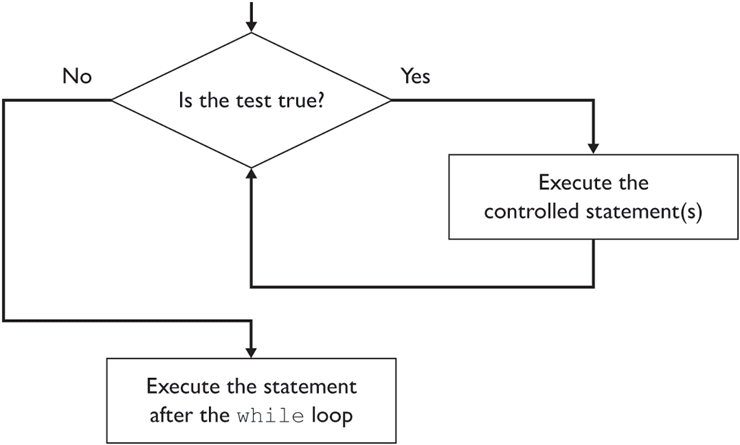
\includegraphics[max width=\linewidth]{Pictures/ch05_p4_img0.png}
\\
\textit{Hình 5.1: Luồng hoạt động của vòng lặp while}

Như Hình 5.1 chỉ ra, vòng lặp \texttt{while} thực hiện kiểm tra điều kiện ở phần đầu của vòng lặp, trước khi thân vòng lặp được thực thi. Một vòng lặp \texttt{while} sẽ không thực thi các câu lệnh được kiểm soát của nó nếu điều kiện của nó đánh giá là \texttt{false} ngay trong lần đầu tiên nó được đánh giá.

Dưới đây là một ví dụ về vòng lặp \texttt{while}:

\begin{verbatim}
int number = 1;
while (number <= 200) {
    number = number * 2;
}
\end{verbatim}

Vòng lặp này khởi tạo một biến số nguyên tên là \texttt{number} bằng 1 và sau đó nhân đôi nó trong khi nó nhỏ hơn hoặc bằng 200. Nhìn bề ngoài, hoạt động này tương tự như việc sử dụng câu lệnh \texttt{if}:

\begin{verbatim}
int number = 1;
if (number <= 200) {
    number = number * 2;
}
\end{verbatim}

Sự khác biệt giữa hai dạng này là vòng lặp \texttt{while} thực thi nhiều lần, lặp lại cho đến khi điều kiện kiểm tra đánh giá là \texttt{false}. Câu lệnh \texttt{if} chỉ thực thi câu lệnh nhân đôi một lần duy nhất, để lại \texttt{number} bằng 2. Vòng lặp \texttt{while} thực thi câu lệnh nhân đôi lặp đi lặp lại, với \texttt{number} nhận các giá trị 1, 2, 4, 8, 16, 32, 64, 128, và 256. Vòng lặp không dừng thực thi cho đến khi điều kiện kiểm tra đánh giá là \texttt{false}. Nó thực thi câu lệnh gán tám lần và kết thúc khi \texttt{number} được đặt thành giá trị 256 (lũy thừa đầu tiên của 2 lớn hơn 200).

Dưới đây là một vòng lặp \texttt{while} chứa hai câu lệnh:

\begin{verbatim}
int number = 1;
while (number <= max) {
    System.out.println("Hi there");
    number++;
}
\end{verbatim}

Vòng lặp \texttt{while} này gần như giống hệt với vòng lặp \texttt{for} sau:

\begin{verbatim}
for (int number = 1; number <= max; number++) {
    System.out.println("Hi there");
}
\end{verbatim}

Sự khác biệt duy nhất giữa hai vòng lặp này là phạm vi hoạt động (scope) của biến \texttt{number}. Trong vòng lặp \texttt{while}, \texttt{number} được khai báo trong phạm vi bên ngoài vòng lặp. Trong vòng lặp \texttt{for}, \texttt{number} được khai báo bên trong vòng lặp.

\subsection*{Vòng lặp tìm ước số nhỏ nhất}
Giả sử bạn muốn tìm ước số nhỏ nhất của một số khác 1. Bảng 5.1 đưa ra các ví dụ về những gì bạn đang tìm kiếm.

\textit{Bảng 5.1: Ví dụ về các ước số}

Dưới đây là mô tả bằng mã giả (pseudocode) về cách bạn có thể tìm giá trị này:

\begin{verbatim}
bắt đầu divisor tại 2.
while (giá trị hiện tại của divisor không chia hết) {
    tăng divisor.
}
\end{verbatim}

Bạn không bắt đầu \texttt{divisor} tại 1 vì bạn đang tìm kiếm ước số đầu tiên lớn hơn 1. Để tinh chỉnh mã giả này, bạn phải rõ ràng hơn về điều gì làm cho một ước số "chia hết". Một ước số của một số sẽ không có số dư khi số đó được chia cho ước số đó. Bạn có thể viết lại quy tắc này dưới dạng mã giả sau:

\begin{verbatim}
bắt đầu divisor tại 2.
while (số dư của number/divisor không bằng 0) {
    tăng divisor.
}
\end{verbatim}

Bài toán này có thể được giải quyết bằng cách sử dụng toán tử chia lấy dư \texttt{\%}, toán tử này cho biết số dư của phép chia số nguyên. Vòng lặp \texttt{while} sau đây thực hiện tác vụ đó:

\begin{verbatim}
int divisor = 2;
while (number % divisor != 0) {
    divisor++;
}
\end{verbatim}

Một vấn đề mà bạn chắc chắn sẽ gặp phải khi viết vòng lặp \texttt{while} là vòng lặp vô hạn (infinite loop) khét tiếng. Hãy xem xét đoạn mã sau:

\begin{verbatim}
int number = 1;
while (number > 0) {
    number++;
}
\end{verbatim}

Bởi vì \texttt{number} bắt đầu là một giá trị dương và vòng lặp làm cho nó lớn hơn, vòng lặp này sẽ tiếp tục vô tận. Bạn phải cẩn thận khi xây dựng các vòng lặp \texttt{while} của mình để tránh các tình huống mà một đoạn mã sẽ không bao giờ kết thúc quá trình thực thi. Mỗi khi bạn viết một vòng lặp \texttt{while}, bạn nên cân nhắc xem khi nào và làm thế nào nó sẽ kết thúc thực thi.

\subsection*{LỖI LẬP TRÌNH PHỔ BIẾN: Vòng lặp vô hạn}
Viết một vòng lặp \texttt{while} không bao giờ kết thúc là điều tương đối dễ mắc phải. Một lý do khiến lỗi này dễ xảy ra là vòng lặp \texttt{while} không có bước cập nhật trong phần đầu của nó như vòng lặp \texttt{for}. Điều quan trọng là lập trình viên phải đưa vào một bước cập nhật chính xác vì bước này là cần thiết để cuối cùng làm cho điều kiện kiểm tra của vòng lặp bị thất bại (trả về \texttt{false}).

Hãy xem xét đoạn mã sau, được thiết kế để yêu cầu người dùng nhập một số và liên tục in ra số đó được giảm đi một nửa cho đến khi đạt đến 0. Lần thử đầu tiên này không biên dịch được:

\begin{verbatim}
Scanner console = new Scanner(System.in);
System.out.print("Type a number: "); 
 
// đoạn mã này không biên dịch được
while (number > 0) {
    int number = console.nextInt();
}
\end{verbatim}
\section{Phần dịch trang 10 đến 20}
\begin{verbatim}
    System.out.println(number / 2);
}
\end{verbatim}

Vấn đề với đoạn mã trước đó là biến \texttt{number} cần phải nằm trong phạm vi hiệu lực (scope) trong quá trình kiểm tra điều kiện của vòng lặp (loop), vì vậy nó không thể được khai báo bên trong vòng lặp. Một nỗ lực không chính xác để khắc phục lỗi biên dịch này là cắt và dán dòng khởi tạo \texttt{number} ra bên ngoài vòng lặp:

\begin{verbatim}
// đoạn mã này có một vòng lặp vô hạn
int number = console.nextInt(); // được di chuyển ra ngoài vòng lặp 
 
while (number > 0) {
    System.out.println(number / 2);
}
\end{verbatim}

Phiên bản này của đoạn mã có một vòng lặp vô hạn (infinite loop); nếu vòng lặp được bắt đầu, nó sẽ không bao giờ kết thúc. Vấn đề này phát sinh vì không có câu lệnh cập nhật nào bên trong thân vòng lặp \texttt{while} để thay đổi giá trị của \texttt{number}. Nếu \texttt{number} lớn hơn 0, vòng lặp sẽ liên tục in ra giá trị của nó và kiểm tra điều kiện vòng lặp, và điều kiện đó sẽ luôn trả về kết quả là \texttt{true}.

Phiên bản dưới đây của đoạn mã sẽ giải quyết vấn đề vòng lặp vô hạn. Vòng lặp chứa một bước cập nhật trong mỗi lần lặp để chia đôi số nguyên và lưu trữ giá trị mới của nó. Nếu số nguyên chưa đạt đến giá trị 0, vòng lặp sẽ tiếp tục:

\begin{verbatim}
// đoạn mã này hoạt động chính xác
int number = console.nextInt(); // được di chuyển ra ngoài vòng lặp
while (number > 0) {
    number = number / 2; // bước cập nhật: chia đôi
    System.out.println(number);
}
\end{verbatim}

Ý tưởng cốt lõi là thân của mỗi vòng lặp \texttt{while} đều nên chứa đoạn mã để cập nhật các số hạng được kiểm tra trong điều kiện vòng lặp. Nếu điều kiện vòng lặp \texttt{while} kiểm tra giá trị của một biến, thân vòng lặp nên gán lại một giá trị mới có ý nghĩa cho biến đó.

\subsection*{Số ngẫu nhiên (Random Numbers)}

Chúng ta thường muốn các chương trình của mình thể hiện các hành vi có vẻ ngẫu nhiên. Ví dụ, chúng ta muốn các chương trình trò chơi tạo ra một con số để người dùng đoán, xáo trộn một bộ bài, chọn một từ trong danh sách để người dùng đoán, v.v. Bản chất của các chương trình máy tính là có thể dự đoán được và không ngẫu nhiên. Nhưng chúng ta có thể tạo ra các giá trị có vẻ như ngẫu nhiên. Những giá trị như vậy được gọi là giả ngẫu nhiên (pseudorandom) vì chúng được tạo ra bằng thuật toán.

\textbf{Số giả ngẫu nhiên (Pseudorandom Numbers)}
\begin{quote}
Những con số mà mặc dù được bắt nguồn từ các thuật toán có thể dự đoán trước và được xác định rõ ràng, nhưng lại mô phỏng các đặc tính của các con số được chọn một cách ngẫu nhiên.
\end{quote}

Java cung cấp một vài cơ chế để có được các số giả ngẫu nhiên. Một lựa chọn là gọi phương thức \texttt{random} từ lớp \texttt{Math} để lấy một giá trị ngẫu nhiên kiểu \texttt{double} có thuộc tính sau:
\[
0.0 \le \text{Math.random()} < 1.0
\]
Phương thức này cung cấp một cách nhanh chóng và dễ dàng để có được một số ngẫu nhiên, và bạn có thể sử dụng phép nhân để thay đổi phạm vi của các số mà phương thức tạo ra. Java cũng cung cấp một lớp gọi là \texttt{Random} giúp sử dụng dễ dàng hơn. Nó được bao gồm trong gói \texttt{java.util}, vì vậy bạn phải khai báo \texttt{import} ở đầu chương trình để sử dụng nó.

Các đối tượng \texttt{Random} có một vài phương thức hữu ích liên quan đến việc tạo số giả ngẫu nhiên, được liệt kê trong Bảng 5.2. Mỗi khi bạn gọi một trong những phương thức này, Java sẽ tạo và trả về một số ngẫu nhiên mới thuộc kiểu dữ liệu được yêu cầu.

\textbf{Bảng 5.2 Các phương thức hữu ích của đối tượng Random}

Để tạo các số ngẫu nhiên, trước tiên bạn cần xây dựng một đối tượng \texttt{Random}:
\begin{verbatim}
Random r = new Random();
\end{verbatim}
Sau đó, bạn có thể gọi phương thức \texttt{nextInt} của nó, truyền vào một số nguyên tối đa. Con số trả về sẽ nằm trong khoảng từ 0 (bao gồm) đến giá trị tối đa đó (không bao gồm). Ví dụ: nếu bạn gọi \texttt{nextInt(100)}, bạn sẽ nhận được một số từ 0 đến 99. Bạn có thể cộng thêm 1 vào số đó để có được phạm vi từ 1 đến 100.

Tương tác JShell sau đây tạo ra một đối tượng \texttt{Random} và sử dụng nó để tạo ra một vài số ngẫu nhiên từ 1 đến 10. Lưu ý rằng mỗi lần gọi \texttt{nextInt} đều tạo ra một số nguyên ngẫu nhiên mới:
\begin{verbatim}
jshell> Random r = new Random();
r ==> java.util.Random@5c7fa833 
 
jshell> r.nextInt(10)
$2 ==> 2 
 
jshell> r.nextInt(10)
$3 ==> 9 
 
jshell> r.nextInt(10)
$4 ==> 9 
 
jshell> r.nextInt(10)
$5 ==> 0 
 
jshell> r.nextInt(10)
$6 ==> 5
\end{verbatim}

Hãy cùng xem một chương trình đơn giản chọn các số từ 1 đến 10 cho đến khi một số cụ thể xuất hiện. Chúng ta sẽ sử dụng một đối tượng \texttt{Random} để tạo ra các số giả ngẫu nhiên.

Vòng lặp của chúng ta sẽ trông giống như thế này (trong đó \texttt{number} là giá trị mà người dùng yêu cầu chúng ta tạo ra):
\begin{verbatim}
int result;
while (result != number) {
    result = r.nextInt(10) + 1; // số ngẫu nhiên từ 1-10

    System.out.println("next number = " + result);
}
\end{verbatim}

Lưu ý rằng chúng ta phải khai báo biến \texttt{result} bên ngoài vòng lặp \texttt{while}, bởi vì \texttt{result} xuất hiện trong phần kiểm tra điều kiện của vòng lặp \texttt{while}. Đoạn mã trên có hướng tiếp cận đúng, nhưng Java sẽ không chấp nhận nó. Đoạn mã sẽ tạo ra một thông báo lỗi rằng biến \texttt{result} có thể chưa được khởi tạo. Đây là một ví dụ về một vòng lặp cần được mồi (priming).

\textbf{Mồi vòng lặp (Priming a Loop)}
\begin{quote}
Khởi tạo các biến trước một vòng lặp để "mồi bơm" và đảm bảo rằng vòng lặp sẽ được thực thi.
\end{quote}

Chúng ta muốn đặt biến \texttt{result} thành một giá trị nào đó để khiến vòng lặp được thực thi, nhưng giá trị cụ thể không quan trọng miễn là nó đưa chúng ta vào được trong vòng lặp. Tuy nhiên, chúng ta cần cẩn thận không đặt nó thành giá trị mà người dùng muốn chúng ta tạo ra. Trong chương trình này, chúng ta đang làm việc với các giá trị từ 1 đến 10, vì vậy chúng ta có thể đặt \texttt{result} thành một giá trị như -1 vốn rõ ràng nằm ngoài phạm vi số này. Đôi khi chúng ta gọi đây là một giá trị "giả" (dummy value) vì chúng ta không thực sự xử lý nó. Ở phần sau của chương trình này, chúng ta sẽ thấy một biến thể của vòng lặp \texttt{while} không yêu cầu kiểu mồi này.

Dưới đây là giải pháp chương trình hoàn chỉnh:
\begin{verbatim}
 1 // Chọn các số ngẫu nhiên từ 1-10 cho đến khi chọn được giá trị đã cho.
 2 import java.util.*;
 3 
 4 public class Pick {
 5     public static void main(String[] args) {
 6         System.out.println("This program picks numbers from");
 7         System.out.println("1 to 10 until a particular");
 8         System.out.println("number comes up.");
 9         System.out.println();
10
11         Scanner console = new Scanner(System.in);
12         Random r = new Random();
13
14         System.out.print("Pick a number between 1 and 10--> ");
15         int number = console.nextInt();
16
17         int result = -1; // đặt thành -1 để đảm bảo chúng ta vào vòng lặp
18         int count = 0;
19         while (result != number) {
20             result = r.nextInt(10) + 1; // số ngẫu nhiên từ 1-10

21             System.out.println("next number = " + result);
22             count++;
23         }
24         System.out.println("Your number came up after " +
25                            count + " times");
26     }
27 }
\end{verbatim}

Tùy thuộc vào chuỗi số được trả về bởi đối tượng \texttt{Random}, chương trình có thể kết thúc việc chọn số đã cho một cách nhanh chóng, như trong kết quả chạy mẫu sau:
\begin{verbatim}
This program picks numbers from 
1 to 10 until a particular 
number comes up. 
 
Pick a number between 1 and 10--> 2 
next number = 7 
next number = 8 
next number = 2 
Your number came up after 3 times
\end{verbatim}

Cũng có khả năng chương trình sẽ mất một khoảng thời gian để chọn được số đó, như trong kết quả chạy mẫu dưới đây:
\begin{verbatim}
This program picks numbers from 
1 to 10 until a particular 
number comes up. 
 
Pick a number between 1 and 10--> 10 
next number = 9 
next number = 7 
next number = 7 
next number = 5 
next number = 8 
next number = 8 
next number = 1 
next number = 5 
next number = 1 
next number = 9 
next number = 7 
next number = 10 
Your number came up after 12 times
\end{verbatim}

\subsection*{LỖI LẬP TRÌNH PHỔ BIẾN}
\textit{Sử dụng sai đối tượng Random}

Một đối tượng \texttt{Random} sẽ chọn một số nguyên ngẫu nhiên mới mỗi khi phương thức \texttt{nextInt} được gọi. Khi sinh viên cố gắng tạo ra một giá trị ngẫu nhiên có điều kiện ràng buộc, chẳng hạn như một số lẻ, đôi khi họ viết nhầm đoạn mã như sau:
\begin{verbatim}
// đoạn mã này chứa một lỗi (bug)
Random r = new Random(); 
 
if (r.nextInt() % 2 == 0) {
    System.out.println("Even number: " + r.nextInt());
} else {
    System.out.println("Odd number: " + r.nextInt());
}
\end{verbatim}

Đoạn mã trên thất bại trong nhiều trường hợp vì đối tượng \texttt{Random} tạo ra một số nguyên ngẫu nhiên để sử dụng trong kiểm tra điều kiện \texttt{if/else}, và sau đó lại tạo một số khác để sử dụng trong bất kỳ câu lệnh \texttt{println} nào được chọn để thực thi. Ví dụ, kiểm tra điều kiện \texttt{if} có thể nhận được giá trị ngẫu nhiên là 47 từ đối tượng \texttt{Random}. Phép thử sẽ thấy rằng $47 \% 2$ không bằng 0, vì vậy đoạn mã sẽ chuyển sang câu lệnh \texttt{else}. Câu lệnh \texttt{println} sau đó sẽ thực thi một lệnh gọi khác tới \texttt{nextInt}, lệnh này sẽ trả về một con số hoàn toàn khác (chẳng hạn như 128). Kết quả đầu ra của đoạn mã khi đó sẽ là câu lệnh kỳ lạ sau:
\section{Phần dịch trang 20 đến 30}
Số lẻ: 128

Giải pháp cho vấn đề này là lưu trữ số nguyên được chọn ngẫu nhiên vào một biến và chỉ gọi lại \texttt{nextInt} khi thực sự cần một số ngẫu nhiên khác. Đoạn mã sau đây thực hiện tác vụ này:

\begin{verbatim}
// đoạn mã này hoạt động chính xác
Random r = new Random();
int n = r.nextInt(); // lưu số ngẫu nhiên vào một biến
if (n % 2 == 0) {
    System.out.println("Even number: " + n);
} else {
    System.out.println("Odd number: " + n);
}
\end{verbatim}

\subsection*{Mô phỏng (Simulations)}

Khoa học và kỹ thuật truyền thống đòi hỏi nhiều sự tương tác trong thế giới thực. Các nhà khoa học tiến hành thực nghiệm để kiểm tra các giả thuyết của họ và các kỹ sư xây dựng các mẫu thử (prototypes) để thử nghiệm các thiết kế của mình. Nhưng ngày càng có nhiều nhà khoa học và kỹ sư tìm đến máy tính như một cách để tăng năng suất bằng cách chạy các mô phỏng (simulations) trước nhằm khám phá các khả năng, trước khi họ tiến hành một thực nghiệm thực tế hoặc xây dựng một mẫu thử thực tế. Một nhà khoa học máy tính nổi tiếng tên là Jeanette Wing đã lập luận rằng việc tăng cường sử dụng tính toán này của các nhà khoa học và kỹ sư sẽ dẫn đến tư duy máy tính (computational thinking) được xem là nền tảng, giống như cách mà việc đọc, viết và làm toán được coi là nền tảng ngày nay.

Dưới góc độ lập trình, hai thành phần chính trong một mô phỏng là các số giả ngẫu nhiên (pseudorandom numbers) và các vòng lặp (loops). Một số mô phỏng có thể được viết bằng cách sử dụng vòng lặp \texttt{for}, nhưng thông thường chúng ta sử dụng vòng lặp \texttt{while} vì mô phỏng cần được chạy vô hạn cho đến khi một điều kiện nào đó được thỏa mãn.

Là một ví dụ đơn giản, chúng ta hãy xem cách mô phỏng việc tung hai con xúc xắc cho đến khi tổng số điểm của chúng bằng 7. Chúng ta có thể sử dụng một đối tượng \texttt{Random} để mô phỏng các con xúc xắc, gọi nó một lần cho mỗi con xúc xắc. Chúng ta muốn lặp lại cho đến khi tổng bằng 7 và có thể in ra các lần tung khác nhau xuất hiện khi chạy mô phỏng. Dưới đây là một thử nghiệm đầu tiên khá tốt:

\begin{verbatim}
Random r = new Random();
while (sum != 7) {
    // tung xúc xắc một lần
    int roll1 = r.nextInt(6) + 1;
    int roll2 = r.nextInt(6) + 1;
    int sum = roll1 + roll2;
    System.out.println(roll1 + " + " + roll2 + " = " + sum);
}
\end{verbatim}

Đoạn mã trên tạo ra lỗi trình biên dịch sau:

\begin{verbatim}
Dice.java:7: error: cannot find symbol
symbol : variable sum
location: class Dice
    while (sum != 7) {
              ^
1 error
\end{verbatim}

Vấn đề là điều kiện kiểm tra vòng lặp \texttt{while} tham chiếu đến biến \texttt{sum}, nhưng biến đó lại được khai báo bên trong thân vòng lặp. Chúng ta không thể khai báo biến trong phạm vi bên trong (inner scope) vì chúng ta cần tham chiếu đến nó trong điều kiện kiểm tra vòng lặp. Vì vậy, chúng ta phải chuyển khai báo biến lên trước vòng lặp. Chúng ta cũng phải gán cho biến một giá trị ban đầu để đảm bảo rằng nó sẽ đi vào vòng lặp. Đoạn mã này là một ví dụ khác về thời điểm chúng ta cần chuẩn bị trước cho vòng lặp (prime the loop):

\begin{verbatim}
Random r = new Random();
int sum = 0; // đặt thành 0 để đảm bảo chúng ta vào vòng lặp
while (sum != 7) {
    // tung xúc xắc một lần
    int roll1 = r.nextInt(6) + 1;
    int roll2 = r.nextInt(6) + 1;
    sum = roll1 + roll2;
    System.out.println(roll1 + " + " + roll2 + " = " + sum);
}
\end{verbatim}

Phiên bản này của đoạn mã biên dịch và hoạt động chính xác. Một kết quả chạy mẫu như sau:

\begin{verbatim}
1 + 4 = 5 
5 + 6 = 11 
1 + 3 = 4 
4 + 3 = 7 
\end{verbatim}

\subsection*{Vòng lặp do/while (do/while Loop)}

Vòng lặp \texttt{while} là vòng lặp không xác định (indefinite loop) tiêu chuẩn, nhưng Java cung cấp một số giải pháp thay thế khác. Phần này trình bày về vòng lặp \texttt{do/while}. Các biến thể khác được bao gồm trong Phụ lục C.

Như chúng ta đã thấy, vòng lặp \texttt{while} kiểm tra điều kiện ở "đỉnh" vòng lặp, trước khi nó thực thi câu lệnh mà nó kiểm soát. Java có một giải pháp thay thế được gọi là vòng lặp \texttt{do/while} kiểm tra điều kiện ở "đáy" vòng lặp. Vòng lặp \texttt{do/while} có cú pháp như sau:

\begin{verbatim}
do {
    <câu lệnh>;
    ...
    <câu lệnh>;
} while (<điều kiện>);
\end{verbatim}

Dưới đây là một số mã mẫu sử dụng vòng lặp \texttt{do/while}:

\begin{verbatim}
int number = 1;
do {
    number *= 2;
} while (number <= 200);
\end{verbatim}

Vòng lặp này tạo ra kết quả giống như vòng lặp \texttt{while} tương ứng, nhân đôi biến \texttt{number} cho đến khi giá trị của nó đạt đến 256, là lũy thừa đầu tiên của 2 lớn hơn 200. Nhưng không giống như vòng lặp \texttt{while}, vòng lặp \texttt{do/while} luôn thực thi các câu lệnh được kiểm soát của nó ít nhất một lần. Sơ đồ trong Hình 5.2 cho thấy luồng điều khiển trong một vòng lặp \texttt{do/while}.

Hình 5.2 Luồng hoạt động của vòng lặp do/while
\begin{center}
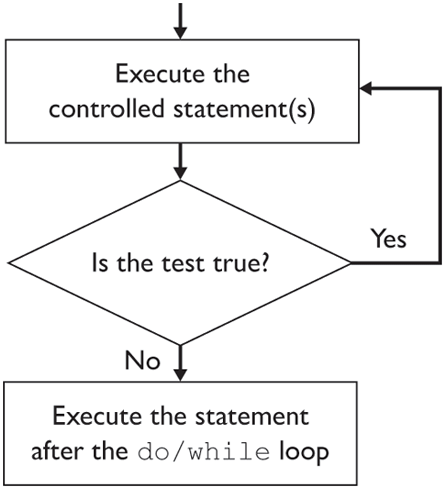
\includegraphics[max width=\linewidth]{Pictures/ch05_p25_img0.png}
\end{center}

Vòng lặp \texttt{do/while} hữu ích nhất trong các tình huống mà bạn biết mình phải thực thi vòng lặp ít nhất một lần. Ví dụ, trong phần trước chúng ta đã viết đoạn mã sau để mô phỏng việc tung hai con xúc xắc cho đến khi bạn có tổng bằng 7:

\begin{verbatim}
Random r = new Random();
int sum = 0; // đặt thành 0 để đảm bảo chúng ta vào vòng lặp
while (sum != 7) {
    // tung xúc xắc một lần
    int roll1 = r.nextInt(6) + 1;
    int roll2 = r.nextInt(6) + 1;
    sum = roll1 + roll2;
    System.out.println(roll1 + " + " + roll2 + " = " + sum);
}
\end{verbatim}

Chúng ta đã phải chuẩn bị trước cho vòng lặp bằng cách đặt \texttt{sum} thành 0 để máy tính đi vào vòng lặp. Với vòng lặp \texttt{do/while}, chúng ta có thể loại bỏ bước chuẩn bị này:

\begin{verbatim}
Random r = new Random();
int sum;
do {
    // tung xúc xắc một lần
    int roll1 = r.nextInt(6) + 1;
    int roll2 = r.nextInt(6) + 1;
    sum = roll1 + roll2;
    System.out.println(roll1 + " + " + roll2 + " = " + sum);
} while (sum != 7);
\end{verbatim}

Trong phiên bản này, chúng ta luôn thực thi thân vòng lặp ít nhất một lần, điều này giúp gán một giá trị cho biến \texttt{sum} trước khi nó đi tới điều kiện kiểm tra vòng lặp hiện xuất hiện ở đáy vòng lặp.

Có nhiều bài toán lập trình mà việc sử dụng vòng lặp \texttt{do/while} là phù hợp. Các vòng lặp này thường hữu ích trong các chương trình tương tác khi bạn biết mình muốn thực hiện một việc gì đó ít nhất một lần. Ví dụ: bạn có thể có một vòng lặp cho phép người dùng chơi một trò chơi nhiều lần; bạn có thể khá chắc chắn rằng người dùng sẽ muốn chơi ít nhất một lần. Tương tự như thế, nếu bạn đang chơi một trò chơi đoán số với người dùng, bạn sẽ luôn phải nhận được ít nhất một lượt đoán.

\subsection*{5.2 Thuật toán hàng rào (Fencepost Algorithms)}

Một bài toán lập trình phổ biến liên quan đến một loại vòng lặp đặc biệt được gọi là vòng lặp hàng rào (fencepost loop). Hãy xem xét bài toán sau: Bạn muốn dựng một hàng rào dài 100 yard, và bạn muốn lắp một cây cột (post) sau mỗi 10 yard. Bạn cần bao nhiêu cây cột? Nếu bạn nhẩm nhanh một phép chia trong đầu, bạn có thể nghĩ rằng mình cần 10 cây cột, nhưng thực tế bạn cần 11 cây cột. Đó là vì hàng rào bắt đầu và kết thúc bằng các cây cột. Nói cách khác, một hàng rào trông giống như Hình 5.3.

Hình 5.3 Một hàng rào điển hình

Vì bạn muốn có cột ở cả ngoài cùng bên trái và ngoài cùng bên phải, bạn không thể sử dụng vòng lặp đơn giản sau đây (nó không dựng cây cột cuối cùng):

\begin{verbatim}
for (chiều dài hàng rào) {
    dựng một cây cột.
    gắn một đoạn dây kẽm.
}
\end{verbatim}

Nếu bạn sử dụng vòng lặp trên, bạn sẽ có một hàng rào trông giống như Hình 5.4.

Hình 5.4 Một hàng rào bị lỗi

Việc thay đổi thứ tự của hai thao tác cũng không giải quyết được vấn đề, bởi vì khi đó bạn sẽ bỏ sót cây cột đầu tiên. Vấn đề với vòng lặp này là nó tạo ra số cây cột bằng đúng số đoạn dây kẽm, nhưng chúng ta biết rằng chúng ta cần thêm một cây cột nữa. Đó là lý do tại sao bài toán này đôi khi còn được gọi là bài toán "vòng lặp rưỡi" (loop and a half) — chúng ta muốn thực thi một nửa vòng lặp này (dựng một cây cột) thêm một lần nữa.
\section{Phần dịch trang 30 đến 40}
Một giải pháp là dựng một trong các cây cột trước hoặc sau vòng lặp (loop). Giải pháp thông thường là thực hiện việc đó trước:

\begin{verbatim}
dựng một cây cột.
for (chiều dài của hàng rào) {
    buộc một sợi dây thép.
    dựng một cây cột.
}
\end{verbatim}


Lưu ý rằng thứ tự của hai thao tác trong thân vòng lặp bây giờ đã được đảo ngược vì cây cột đầu tiên được dựng trước khi đi vào vòng lặp.

Một ví dụ đơn giản, hãy xem xét bài toán in ra các số nguyên từ 1 đến 10, phân tách bằng dấu phẩy. Nói cách khác, chúng ta muốn có kết quả đầu ra sau:
 
\begin{verbatim}
1, 2, 3, 4, 5, 6, 7, 8, 9, 10 
\end{verbatim}


Nhiệm vụ này là một bài toán hàng rào (fencepost problem) kinh điển vì chúng ta muốn in ra 10 con số nhưng chỉ có 9 dấu phẩy. Theo thuật ngữ hàng rào của chúng ta, việc ghi một con số là phần ``cột'' (post) của nhiệm vụ và ghi một dấu phẩy là phần ``dây thép'' (wire). Vì vậy, triển khai mã giả (pseudocode) mà chúng ta đã xây dựng, chúng ta in số đầu tiên trước vòng lặp và đảo ngược thứ tự các thao tác bên trong vòng lặp bằng cách in một dấu phẩy trước một con số:

\begin{verbatim}
System.out.print(1);
for (int i = 2; i <= 10; i++) {
    System.out.print(", " + i);
}
System.out.println();
\end{verbatim}


\subsection*{Hàng rào với if}

Nhiều vòng lặp hàng rào mà bạn viết sẽ yêu cầu thực thi có điều kiện. Trên thực tế, bản thân bài toán hàng rào có thể được giải quyết bằng một câu lệnh \texttt{if}. Hãy nhớ rằng giải pháp kinh điển cho bài toán hàng rào là xử lý cây cột đầu tiên trước khi vòng lặp bắt đầu:

\begin{verbatim}
dựng một cây cột.
for (chiều dài của hàng rào) {
    buộc một sợi dây thép.
    dựng một cây cột.
}
\end{verbatim}


Giải pháp này giải quyết được vấn đề, nhưng nó có thể gây bối rối vì bên trong vòng lặp, các bước dường như có thứ tự ngược lại. Bạn có thể sử dụng một câu lệnh \texttt{if} và giữ nguyên thứ tự ban đầu của các bước:

\begin{verbatim}
for (chiều dài của hàng rào) {
    dựng một cây cột.
    if (đây không phải là cây cột cuối cùng) {
        buộc một sợi dây thép.
    }
}
\end{verbatim}


Biến thể này không được sử dụng thường xuyên như giải pháp kinh điển vì nó liên quan đến cả điều kiện kiểm tra vòng lặp và điều kiện kiểm tra bên trong vòng lặp. Thường thì các kiểm tra này gần như giống hệt nhau, vì vậy việc kiểm tra cùng một thứ hai lần mỗi khi vòng lặp thực thi là không hiệu quả. Nhưng sẽ có những tình huống mà bạn có thể sử dụng cách tiếp cận này. Ví dụ, trong cách tiếp cận kinh điển, các dòng mã tương ứng với việc dựng một cây cột bị lặp lại. Nếu bạn đang viết một chương trình mà bước này đòi hỏi nhiều mã, bạn có thể quyết định rằng việc đặt câu lệnh \texttt{if} bên trong vòng lặp là một cách tiếp cận tốt hơn, ngay cả khi nó dẫn đến một số kiểm tra bổ sung.

Ví dụ, hãy xem xét việc viết một phương thức gọi là \texttt{multiprint} để in một chuỗi với một số lần cụ thể. Giả sử bạn muốn kết quả đầu ra nằm trên một dòng riêng biệt, bên trong dấu ngoặc vuông và được phân tách bằng dấu phẩy. Dưới đây là hai lệnh gọi ví dụ:

\begin{verbatim}
multiprint("please", 4);
multiprint("beetlejuice", 3);
\end{verbatim}


Bạn kỳ vọng những lệnh gọi này sẽ tạo ra kết quả đầu ra sau:
 
\begin{verbatim}
[please, please, please, please] 
[beetlejuice, beetlejuice, beetlejuice] 
\end{verbatim}


Nỗ lực đầu tiên của bạn trong việc viết phương thức này có thể là một vòng lặp đơn giản in các dấu ngoặc vuông bên ngoài vòng lặp và in chuỗi cùng dấu phẩy bên trong vòng lặp:

\begin{verbatim}
public static void multiprint(String s, int times) {
    System.out.print("[");
    for (int i = 1; i <= times; i++) {
        System.out.print(s + ", ");
    }
    System.out.println("]");
}
\end{verbatim}


Rất tiếc, đoạn mã này tạo ra một dấu phẩy thừa sau giá trị cuối cùng:
 
\begin{verbatim}
[please, please, please, please, ] 
[beetlejuice, beetlejuice, beetlejuice, ] 
\end{verbatim}


Bởi vì dấu phẩy là ký tự phân tách, bạn muốn số chuỗi in ra nhiều hơn số dấu phẩy một đơn vị (ví dụ: hai dấu phẩy để phân tách ba lần xuất hiện của ``beetlejuice''). Bạn có thể sử dụng giải pháp kinh điển cho bài toán hàng rào để đạt được hiệu ứng này bằng cách in một chuỗi bên ngoài vòng lặp và đảo ngược thứ tự in bên trong vòng lặp:

\begin{verbatim}
public static void multiprint(String s, int times) {
    System.out.print("[" + s);
    for (int i = 2; i <= times; i++) {
        System.out.print(", " + s);
    }
    System.out.println("]");
}
\end{verbatim}


Lưu ý rằng vì bạn đang in một trong các chuỗi trước khi vòng lặp bắt đầu, bạn phải sửa đổi vòng lặp để nó không in nhiều chuỗi như trước nữa. Việc điều chỉnh biến vòng lặp \texttt{i} bắt đầu từ hai sẽ bù cho giá trị đầu tiên được in trước vòng lặp.

Rất tiếc, giải pháp này cũng hoạt động không chính xác. Hãy xem xét điều gì xảy ra khi bạn yêu cầu phương thức in một chuỗi không lần (0 lần), như trong:

\begin{verbatim}
multiprint("please don't", 0);
\end{verbatim}


Lệnh gọi này tạo ra kết quả đầu ra không chính xác sau:
 
\begin{verbatim}
[please don't] 
\end{verbatim}


Bạn muốn người dùng có thể yêu cầu xuất hiện không lần một chuỗi, vì vậy phương thức không nên tạo ra kết quả đầu ra không chính xác đó. Vấn đề là giải pháp kinh điển cho bài toán hàng rào liên quan đến việc in một giá trị trước khi vòng lặp bắt đầu. Để phương thức hoạt động chính xác cho trường hợp bằng không, bạn có thể bao gồm một câu lệnh \texttt{if/else}:

\begin{verbatim}
public static void multiprint(String s, int times) {
    if (times == 0) {
        System.out.println("[]");

    } else {
        System.out.print("[" + s);
        for (int i = 2; i <= times; i++) {
            System.out.print(", " + s);
        }
        System.out.println("]");
    }
}
\end{verbatim}


Ngoài ra, bạn có thể bao gồm một câu lệnh \texttt{if} bên trong vòng lặp (cách tiếp cận kiểm tra kép):

\begin{verbatim}
public static void multiprint(String s, int times) {
    System.out.print("[");
    for (int i = 1; i <= times; i++) {
        System.out.print(s);
        if (i < times) {
            System.out.print(", ");
        }
    }
    System.out.println("]");
}
\end{verbatim}


Mặc dù phiên bản mã trước đó thực hiện một phép kiểm tra tương tự hai lần trong mỗi lần lặp, nhưng nó đơn giản hơn so với việc sử dụng giải pháp hàng rào kinh điển và trường hợp đặc biệt của nó. Không có giải pháp nào tốt hơn giải pháp nào, vì luôn có sự đánh đổi. Nếu bạn nghĩ rằng mã sẽ được thực thi thường xuyên và vòng lặp sẽ lặp lại nhiều lần, bạn có thể có xu hướng sử dụng giải pháp hiệu quả hơn. Ngược lại, bạn có thể chọn mã đơn giản hơn.

\subsection*{Vòng lặp Sentinel (Sentinel Loops)}

Giả sử bạn muốn đọc một loạt số từ người dùng và tính tổng của chúng. Bạn có thể hỏi trước người dùng xem cần đọc bao nhiêu số, như chúng ta đã làm trong chương trước, nhưng điều đó không phải lúc nào cũng thuận tiện. Điều gì sẽ xảy ra nếu người dùng có một danh sách dài các số cần nhập và chưa đếm chúng? Một cách để tránh việc hỏi số lượng là chọn một giá trị nhập đặc biệt để báo hiệu kết thúc nhập liệu. Chúng tôi gọi đây là giá trị lính canh (sentinel value).

\paragraph{Sentinel (Lính canh)}
Một giá trị đặc biệt báo hiệu kết thúc nhập liệu.

Ví dụ, bạn có thể yêu cầu người dùng nhập giá trị $-1$ để dừng nhập số. Nhưng làm thế nào để bạn cấu trúc mã của mình để sử dụng lính canh này? Nói chung, bạn sẽ muốn sử dụng cách tiếp cận sau:

\begin{verbatim}
sum = 0.
while (chúng ta chưa thấy lính canh) {
    nhắc và đọc giá trị.
    cộng nó vào tổng.
}
\end{verbatim}


Cách tiếp cận này không hoàn toàn hoạt động tốt. Ví dụ, giả sử người dùng nhập các số $10$, $42$, $5$ và $-1$. Như mã giả chỉ ra, chúng ta sẽ nhắc và đọc từng giá trị trong số bốn giá trị này rồi cộng chúng vào tổng cho đến khi gặp giá trị lính canh $-1$. Chúng ta khởi tạo tổng bằng $0$, vì vậy phép tính này tính $(10 + 42 + 5 + (-1))$, bằng $56$. Nhưng câu trả lời đúng phải là $57$. Giá trị lính canh $-1$ không được phép tính vào tổng.

Bài toán này là một bài toán hàng rào (fencepost) hoặc ``vòng lặp rưỡi'' (loop-and-a-half) kinh điển: Bạn muốn nhắc và đọc một loạt số, bao gồm cả lính canh, và bạn muốn cộng hầu hết các số lại, nhưng bạn không muốn cộng lính canh vào tổng.

Giải pháp hàng rào thông thường hoạt động hiệu quả: Chúng ta chèn câu lệnh nhắc-và-đọc đầu tiên trước vòng lặp và đảo ngược thứ tự của hai bước trong thân vòng lặp:

\begin{verbatim}
sum = 0.
nhắc và đọc giá trị.
while (chúng ta chưa thấy lính canh) {
    cộng nó vào tổng.
    nhắc và đọc giá trị.
}
\end{verbatim}


Sau đó, bạn có thể tinh chỉnh mã giả này bằng cách đưa vào một biến cho số được đọc từ người dùng:

\begin{verbatim}
sum = 0.
nhắc và đọc một giá trị vào n.
while (n không phải là lính canh) {
    cộng n vào tổng.
\end{verbatim}


\section{Phần dịch trang 40 đến 50}
yêu cầu nhập và đọc một giá trị vào n.


Đoạn mã giả (pseudocode) này được chuyển đổi khá dễ dàng sang mã Java như sau:

\begin{verbatim}
Scanner console = new Scanner(System.in);
int sum = 0;
System.out.print("next integer (–1 to quit)? ");
int number = console.nextInt();
while (number != –1) {
    sum += number;
    System.out.print("next integer (–1 to quit)? ");
    number = console.nextInt();
}
System.out.println("sum = " + sum);
\end{verbatim}


Khi đoạn mã trên được thực thi, quá trình tương tác có thể trông như thế này:

\begin{verbatim}
next integer (–1 to quit)? 10 
next integer (–1 to quit)? 20 
next integer (–1 to quit)? 30 
next integer (–1 to quit)? 40 
next integer (–1 to quit)? 50 
\end{verbatim}

next integer (–1 to quit)? 60 
next integer (–1 to quit)? –1 
sum = 210 


Một số học sinh nhận thấy rằng chương trình sẽ hoạt động tương tự nếu thay vì có một câu lệnh nhắc và đọc trước khi vòng lặp (loop) bắt đầu, chúng ta lại khởi tạo biến \texttt{number} bằng 0. Điều đó đúng trong trường hợp đặc biệt này, nhưng nó không mang tính tổng quát. Ví dụ, nếu bạn muốn tính giá trị lớn nhất (maximum) hoặc nhỏ nhất (minimum), bạn sẽ không muốn đưa số 0 vào làm một giá trị để xem xét. Vì vậy, mặc dù đoạn mã cụ thể này có thể được đơn giản hóa, chúng tôi vẫn muốn trình bày một giải pháp hoạt động hiệu quả cho tất cả các tác vụ tích lũy (cumulative tasks).

\subsection*{5.3 Kiểu boolean (The boolean Type)}

George Boole là một nhà logic học xuất sắc đến nỗi Java đã đặt tên một kiểu dữ liệu theo tên ông. Kiểu dữ liệu \texttt{boolean} trong Java được sử dụng để mô tả các mối quan hệ logic đúng/sai (true/false). Hãy nhớ lại rằng \texttt{boolean} là một trong các kiểu dữ liệu nguyên thủy (primitive types), giống như \texttt{int}, \texttt{double}, và \texttt{char}.

Những người mới bắt đầu thường thắc mắc tại sao các nhà khoa học máy tính lại quan tâm đến logic nhiều đến vậy. Câu trả lời là logic là nền tảng của ngành máy tính giống như vật lý là nền tảng của ngành kỹ thuật. Các kỹ sư học vật lý vì họ muốn chế tạo các vật thể trong thế giới thực vốn bị chi phối bởi các định luật vật lý. Nếu bạn không hiểu vật lý, bạn có khả năng sẽ xây dựng một cây cầu bị sập. Các nhà khoa học máy tính cũng xây dựng các sản phẩm, nhưng trong một thế giới ảo bị chi phối bởi các định luật logic. Nếu bạn không hiểu logic, bạn có khả năng sẽ viết ra các chương trình máy tính bị đổ vỡ.

Mà không hề nhận ra, bạn đã sử dụng các giá trị boolean rồi. Tất cả các cấu trúc điều khiển mà chúng ta đã xem xét—câu lệnh \texttt{if/else}, vòng lặp \texttt{for} (for loops), và vòng lặp \texttt{while} (while loops)—đều được điều khiển bởi các biểu thức xác định các điều kiện kiểm tra. Ví dụ, biểu thức
\begin{verbatim}
number % 2 == 0
\end{verbatim}

là một phép kiểm tra tính chia hết cho 2. Nó cũng là một biểu thức Boolean. Các biểu thức Boolean được thiết kế để nắm bắt các khái niệm về tính đúng và sai, vì vậy không có gì ngạc nhiên khi miền giá trị của kiểu \texttt{boolean} chỉ có hai giá trị: \texttt{true} (đúng) và \texttt{false} (sai). Các từ \texttt{true} và \texttt{false} là các từ khóa dành riêng (reserved words) trong Java. Chúng là các giá trị hằng (literals) của kiểu \texttt{boolean}. Tất cả các biểu thức Boolean, khi được đánh giá, sẽ trả về một trong hai giá trị hằng này. Đừng nhầm lẫn các giá trị đặc biệt này với các hằng chuỗi (string literals) \texttt{"true"} và \texttt{"false"}. Bạn không cần dấu ngoặc kép để tham chiếu đến các hằng Boolean.

Khi bạn viết một chương trình xử lý các giá trị số, bạn thường muốn tính toán một giá trị và lưu trữ nó vào một biến hoặc viết một phương thức (method) để thể hiện một công thức phức tạp nào đó. Chúng ta cũng làm điều tương tự với kiểu \texttt{boolean}. Chúng ta có thể muốn ghi lại một giá trị Boolean vào một biến và chúng ta thường viết các phương thức trả về kết quả Boolean. Ví dụ, chúng ta đã thấy lớp \texttt{String} có các phương thức trả về kết quả Boolean, bao gồm \texttt{startsWith}, \texttt{endsWith}, \texttt{equals}, và \texttt{equalsIgnoreCase}.

Để hiểu rõ hơn về điều này, hãy nhớ lại ý nghĩa của các thuật ngữ này đối với kiểu \texttt{int}. Các hằng (literals) của kiểu \texttt{int} bao gồm \texttt{0}, \texttt{1}, \texttt{2}, v.v. Bởi vì đây là các hằng của kiểu \texttt{int}, bạn có thể viết các biểu thức như sau với chúng:
\begin{verbatim}
int number1 = 1;
int number2 = 0;
\end{verbatim}


Hãy xem xét những gì bạn có thể làm với các biến kiểu \texttt{boolean}. Giả sử bạn định nghĩa hai biến \texttt{boolean}, \texttt{test1} và \texttt{test2}. Các biến này chỉ có thể nhận hai giá trị khả dĩ: \texttt{true} và \texttt{false}. Bạn có thể viết:
\begin{verbatim}
boolean test1 = true;
boolean test2 = false;
\end{verbatim}


Bạn cũng có thể viết một câu lệnh sao chép giá trị của một biến \texttt{boolean} này sang một biến khác, giống như với các biến thuộc bất kỳ kiểu dữ liệu nào khác:
\begin{verbatim}
test1 = test2;
\end{verbatim}


Hơn nữa, bạn biết rằng câu lệnh gán có thể sử dụng các biểu thức như:
\begin{verbatim}
number1 = 2 + 2;
\end{verbatim}

và rằng các phép kiểm tra đơn giản mà bạn đã và đang sử dụng là các biểu thức Boolean. Điều đó có nghĩa là bạn có thể viết các câu lệnh như sau:
\begin{verbatim}
test1 = (2 + 2 == 4);
test2 = (3 * 100 < 250);
\end{verbatim}


Các câu lệnh gán này, về mặt hiệu quả, có nghĩa là "Hãy đặt biến boolean này theo giá trị chân trị được trả về bởi phép kiểm tra sau." Câu lệnh đầu tiên đặt biến \texttt{test1} thành \texttt{true}, vì phép kiểm tra được đánh giá là đúng (\texttt{true}). Câu lệnh thứ hai đặt biến \texttt{test2} thành \texttt{false}, vì phép kiểm tra thứ hai được đánh giá là sai (\texttt{false}). Bạn không cần phải đưa vào các dấu ngoặc đơn, nhưng chúng làm cho các câu lệnh dễ đọc hơn. Rõ ràng, phép gán là một trong những thao tác bạn có thể thực hiện trên các biến kiểu \texttt{boolean}.

\subsection*{Toán tử logic (Logical Operators)}

Trong Java, bạn có thể tạo ra các biểu thức Boolean phức tạp bằng cách sử dụng các toán tử logic (logical operators), được hiển thị trong Bảng 5.3.

\noindent \textbf{Bảng 5.3: Các toán tử logic}

Toán tử phủ định NOT (\texttt{!}) đảo ngược giá trị chân trị của toán hạng của nó. Nếu một biểu thức có giá trị là \texttt{true}, phép phủ định của nó sẽ có giá trị là \texttt{false}, và ngược lại. Bạn có thể biểu diễn mối quan hệ này trong một bảng chân trị (truth table). Bảng chân trị sau đây có hai cột, một cột dành cho biến và một cột dành cho phủ định của nó. Đối với mỗi giá trị của biến, bảng hiển thị giá trị tương ứng của phép phủ định.

\noindent \textbf{Bảng chân trị cho phép phủ định NOT (\texttt{!})}

Ngoài toán tử phủ định, có hai phép liên kết logic mà bạn sẽ sử dụng là AND (\texttt{\&\&}) và OR (\texttt{||}). Bạn sử dụng các liên kết này để ràng buộc hai biểu thức Boolean lại với nhau, tạo ra một biểu thức Boolean mới. Bảng chân trị sau đây cho thấy toán tử AND chỉ được đánh giá là \texttt{true} khi cả hai toán hạng riêng lẻ của nó đều là \texttt{true}.

\noindent \textbf{Bảng chân trị cho phép AND (\texttt{\&\&})}

Bảng chân trị sau đây cho thấy toán tử OR được đánh giá là \texttt{true} ngoại trừ khi cả hai toán hạng đều là \texttt{false}.

\noindent \textbf{Bảng chân trị cho phép OR (\texttt{||})}

Toán tử OR trong Java có ý nghĩa hơi khác một chút so với từ "or" (hoặc) trong tiếng Anh thông thường. Trong tiếng Anh, bạn nói: "Tối nay tôi sẽ học bài hoặc tôi sẽ đi xem phim." Một trong hai điều sẽ đúng, nhưng không phải cả hai. Toán tử OR giống với cụm từ "và/hoặc" (and/or) hơn: Nếu một hoặc cả hai toán hạng là \texttt{true}, thì toàn bộ mệnh đề là \texttt{true}.

Bạn thường sử dụng các toán tử logic khi những gì bạn cần biểu diễn không thể rút gọn thành một phép kiểm tra đơn lẻ. Ví dụ, như chúng ta đã thấy ở chương trước, nếu bạn muốn thực hiện một thao tác cụ thể khi một số nằm trong khoảng từ 1 đến 10, bạn có thể viết:
\begin{verbatim}
if (number >= 1) {
    if (number <= 10) {
        doSomething();
    }
\end{verbatim}


Nhưng bạn có thể diễn đạt điều này dễ dàng hơn bằng cách sử dụng toán tử logic AND:
\begin{verbatim}
if (number >= 1 && number <= 10) {
    doSomething();
\end{verbatim}


Mọi người sử dụng các từ "và" và "hoặc" mọi lúc, nhưng Java chỉ cho phép bạn sử dụng chúng theo nghĩa logic chặt chẽ. Hãy cẩn thận để không viết mã như sau:
\begin{verbatim}
// đoạn mã này không biên dịch được
if (x == 1 || 2 || 3) {
    doSomething();
\end{verbatim}


Trong tiếng Anh thông thường, chúng ta sẽ đọc câu này là "x bằng 1 hoặc 2 hoặc 3", điều này có lý với chúng ta, nhưng lại không có nghĩa đối với Java. Bạn cũng có thể bị cám dỗ viết đoạn mã như sau:
\begin{verbatim}
// đoạn mã này không biên dịch được
if (1 <= x <= 10) {
    doSomethingElse();
\end{verbatim}


Trong toán học, biểu thức này sẽ có nghĩa và sẽ kiểm tra xem \texttt{x} có nằm trong khoảng từ 1 đến 10 (bao gồm cả hai đầu mút) hay không. Tuy nhiên, biểu thức này không có nghĩa trong Java.

Bạn chỉ có thể sử dụng các toán tử logic AND và OR để kết hợp một chuỗi các biểu thức Boolean. Nếu không, máy tính sẽ không hiểu ý bạn muốn diễn đạt. Để biểu diễn ý tưởng "1 hoặc 2 hoặc 3", hãy kết hợp ba biểu thức Boolean khác nhau bằng các toán tử logic OR:
\begin{verbatim}
if (x == 1 || x == 2 || x == 3) {
    doSomething();
\end{verbatim}


Để biểu diễn ý tưởng "nằm trong khoảng từ 1 đến 10 bao gồm cả hai đầu mút", hãy kết hợp hai biểu thức Boolean bằng một toán tử logic AND:
\begin{verbatim}
if (1 <= x && x <= 10) {
    doSomethingElse();
\end{verbatim}


Bây giờ chúng ta đã tìm hiểu về các toán tử logic AND, OR, và NOT, đã đến lúc xem xét lại bảng thứ tự ưu tiên (precedence table) của chúng ta. Toán tử NOT xuất hiện ở trên cùng, với mức độ ưu tiên cao nhất. Hai toán tử logic còn lại có mức độ ưu tiên khá thấp, thấp hơn các toán tử số học và quan hệ nhưng cao hơn các toán tử gán. Toán tử AND có mức độ ưu tiên cao hơn một chút so với toán tử OR. Bảng 5.4 bao gồm các toán tử mới này.

\noindent \textbf{Bảng 5.4: Thứ tự ưu tiên của toán tử trong Java}
\section{Phần dịch trang 50 đến 60}
Theo các quy tắc thứ tự ưu tiên này, khi Java đánh giá một biểu thức như biểu thức dưới đây, máy tính sẽ đánh giá toán tử NOT trước, tiếp theo là AND, và sau đó là OR.

\begin{verbatim}
if (test1 || !test2 && test3) {
    doSomething();
}
\end{verbatim}

\subsection*{Đánh giá ngắn mạch (Short-Circuited Evaluation)}

Trong phần này, chúng ta sẽ khám phá việc sử dụng các toán tử logic để giải quyết một tác vụ lập trình phức tạp, và chúng ta sẽ giới thiệu một thuộc tính quan trọng của các toán tử này. Chúng ta sẽ viết một phương thức tên là \texttt{firstWord} nhận vào một \texttt{String} làm tham số và trả về từ đầu tiên trong chuỗi đó. Để mọi thứ đơn giản, chúng ta quy ước rằng một \texttt{String} được phân tách thành các từ riêng lẻ bằng các khoảng trắng. Nếu \texttt{String} hoàn toàn không có từ nào, phương thức sẽ trả về một chuỗi rỗng. Dưới đây là một số ví dụ gọi hàm:

Hãy nhớ rằng chúng ta có thể gọi phương thức \texttt{substring} để trích xuất một phần của chuỗi. Chúng ta truyền hai tham số vào phương thức \texttt{substring}: chỉ số bắt đầu (starting index) của chuỗi con và chỉ số lớn hơn chỉ số kết thúc một đơn vị. Nếu chuỗi được lưu trữ trong một biến tên là \texttt{s}, nhiệm vụ của chúng ta cơ bản được rút gọn thành các bước sau:
\begin{itemize}
    \item đặt \texttt{start} thành chỉ số đầu tiên của từ.
    \item đặt \texttt{stop} thành chỉ số ngay sau từ đó.
    \item trả về \texttt{s.substring(start, stop)}.
\end{itemize}

Để tiếp cận bước đầu, hãy giả định rằng chỉ số bắt đầu là 0. Chỉ số bắt đầu này sẽ không hoạt động đối với các chuỗi bắt đầu bằng các khoảng trắng, nhưng nó sẽ cho phép chúng ta tập trung vào bước thứ hai trong mã giả (pseudocode).

Hãy xem xét một chuỗi bắt đầu bằng \texttt{"four score"}. Nếu chúng ta kiểm tra các ký tự riêng lẻ của chuỗi và chỉ số của chúng, chúng ta sẽ thấy mẫu sau:

Chúng ta đặt \texttt{start} thành 0. Chúng ta muốn đặt biến \texttt{stop} thành chỉ số ngay sau từ đầu tiên kết thúc. Trong ví dụ này, từ chúng ta muốn lấy là \texttt{"four"}, và nó kéo dài từ chỉ số 0 đến 3. Vì vậy, nếu chúng ta muốn biến \texttt{stop} lớn hơn chỉ số kết thúc một đơn vị, chúng ta muốn đặt nó thành chỉ số 4, vị trí của khoảng trắng đầu tiên trong chuỗi.

Vậy làm thế nào để chúng ta tìm thấy khoảng trắng đầu tiên trong chuỗi? Chúng ta sử dụng một vòng lặp (loop) \texttt{while}. Chúng ta chỉ cần bắt đầu từ đầu chuỗi và lặp cho đến khi gặp một khoảng trắng:
\begin{itemize}
    \item đặt \texttt{stop} thành 0.
    \item trong khi (ký tự tại chỉ số \texttt{stop} không phải là khoảng trắng) \{
    \begin{itemize}
        \item tăng \texttt{stop} lên 1.
    \end{itemize}
    \}
\end{itemize}

Điều này có thể dễ dàng chuyển đổi thành mã Java. Kết hợp nó với giả định của chúng ta rằng \texttt{start} sẽ bằng 0, chúng ta có:

\begin{verbatim}
public static String firstWord(String s) {
    int start = 0;
    int stop = 0;
    while (s.charAt(stop) != ' ') {
        stop++;
    }
    return s.substring(start, stop);
}
\end{verbatim}

Phiên bản này của phương thức hoạt động trong nhiều trường hợp, bao gồm cả chuỗi mẫu của chúng ta, nhưng nó không hoạt động với mọi chuỗi. Nó có hai hạn chế lớn. Chúng ta đã bắt đầu bằng cách giả định rằng chuỗi không bắt đầu bằng khoảng trắng, vì vậy chúng ta biết mình phải khắc phục hạn chế đó.

Vấn đề thứ hai là phiên bản \texttt{firstWord} này không hoạt động trên các chuỗi chỉ có một từ. Ví dụ, nếu chúng ta thực thi nó với một chuỗi như \texttt{"four"}, nó sẽ tạo ra một ngoại lệ \texttt{StringIndex\allowbreak{}OutOfBounds\allowbreak{}Exception} chỉ ra rằng 4 không phải là một chỉ số hợp lệ. Ngoại lệ xảy ra vì mã của chúng ta giả định rằng cuối cùng chúng ta sẽ tìm thấy một khoảng trắng, nhưng không có khoảng trắng nào trong chuỗi \texttt{"four"}. Vì vậy, \texttt{stop} được tăng lên cho đến khi bằng 4, và một ngoại lệ được ném ra vì không có ký tự nào ở chỉ số 4. Điều này đôi khi được gọi là ``vượt quá giới hạn cuối của chuỗi'' (running off the end of the string).

Để giải quyết vấn đề này, chúng ta cần kết hợp một điều kiện kiểm tra liên quan đến độ dài của chuỗi. Nhiều người mới học lập trình cố gắng thực hiện điều này bằng cách sử dụng một số sự kết hợp của \texttt{while} và \texttt{if}, như trong đoạn mã sau:

\begin{verbatim}
int stop = 0;
while (stop < s.length()) {
    if (s.charAt(stop) != ' ') {
       stop++;
    }
}
\end{verbatim}

Đoạn mã này hoạt động đối với các chuỗi một từ như \texttt{"four"} vì ngay khi \texttt{stop} bằng độ dài của chuỗi, chúng ta sẽ thoát ra khỏi vòng lặp. Tuy nhiên, nó không hoạt động đối với các trường hợp nhiều từ ban đầu như \texttt{"four score"}. Chúng ta kết thúc trong một vòng lặp vô hạn (infinite loop) vì một khi \texttt{stop} bằng 4, chúng ta ngừng tăng nó, nhưng chúng ta lại bị mắc kẹt bên trong vòng lặp vì điều kiện kiểm tra yêu cầu tiếp tục miễn là \texttt{stop} nhỏ hơn độ dài của chuỗi. Cách tiếp cận đặt một câu lệnh \texttt{if} bên trong một vòng lặp \texttt{while} này đã dẫn đến một lỗi nổi tiếng thế giới vào ngày 31 tháng 12 năm 2008, khi các máy nghe nhạc Zune trên toàn thế giới ngừng hoạt động (xem Bài tập tự kiểm tra 21 để biết thêm chi tiết).

Điểm cần nhận ra là trong trường hợp này chúng ta cần sử dụng hai điều kiện khác nhau để kiểm soát vòng lặp. Chúng ta chỉ muốn tiếp tục tăng \texttt{stop} nếu chúng ta biết rằng mình chưa gặp khoảng trắng và chưa đi đến cuối chuỗi. Chúng ta có thể thể hiện ý tưởng đó bằng cách sử dụng toán tử logic AND (\texttt{\&\&}):

\begin{verbatim}
int stop = 0;
while (s.charAt(stop) != ' ' && stop < s.length()) {
    stop++;
}
\end{verbatim}

Thật không may, ngay cả điều kiện kiểm tra này cũng không hoạt động. Nó thể hiện đúng hai điều kiện, vì chúng ta muốn đảm bảo rằng mình chưa gặp khoảng trắng và chúng ta muốn đảm bảo rằng mình chưa đi đến cuối chuỗi. Nhưng hãy nghĩ xem điều gì xảy ra ngay khi chúng ta chạm đến cuối chuỗi. Giả sử \texttt{s} là \texttt{"four"} và \texttt{stop} bằng 3.

Chúng ta thấy ký tự tại chỉ số 3 không phải là khoảng trắng và chúng ta thấy \texttt{stop} nhỏ hơn độ dài của chuỗi, vì vậy chúng ta tăng thêm một lần nữa và \texttt{stop} trở thành 4. Khi chúng ta quay lại vòng lặp, chúng ta kiểm tra xem \texttt{s.charAt(4)} có phải là khoảng trắng hay không. Việc kiểm tra này ném ra một ngoại lệ vì chỉ số nằm ngoài giới hạn. Chúng ta cũng kiểm tra xem \texttt{stop} có nhỏ hơn 4 hay không, điều này không đúng, nhưng việc kiểm tra đó diễn ra quá muộn để tránh ngoại lệ.

Java cung cấp một giải pháp cho tình huống này. Các toán tử logic \texttt{\&\&} và \texttt{||} sử dụng cơ chế đánh giá ngắn mạch (short-circuited evaluation).

\paragraph{Đánh giá ngắn mạch (Short-Circuited Evaluation)}
Thuộc tính của các toán tử logic \texttt{\&\&} và \texttt{||} giúp ngăn toán hạng thứ hai bị đánh giá nếu kết quả tổng thể đã rõ ràng từ giá trị của toán hạng đầu tiên.

Trong trường hợp của chúng ta, chúng ta đang thực hiện hai kiểm tra khác nhau và yêu cầu phép AND logic của hai kiểm tra đó. Nếu một trong hai kiểm tra thất bại, kết quả tổng thể sẽ là \texttt{false}, vì vậy nếu kiểm tra đầu tiên thất bại, không cần thiết phải thực hiện kiểm tra thứ hai. Do đánh giá ngắn mạch—nghĩa là vì kết quả tổng thể đã rõ ràng từ kiểm tra đầu tiên—chúng ta hoàn toàn không thực hiện kiểm tra thứ hai. Nói cách khác, việc thực hiện và đánh giá kiểm tra thứ hai bị ngăn chặn (ngắn mạch) bởi thực tế là kiểm tra đầu tiên đã thất bại.

Điều này có nghĩa là chúng ta cần đảo ngược thứ tự của hai kiểm tra này:

\begin{verbatim}
int stop = 0;
while (stop < s.length() && s.charAt(stop) != ' ') {
    stop++;
}
\end{verbatim}

Nếu chúng ta chạy lại kịch bản tương tự với \texttt{stop} bằng 3, chúng ta vượt qua cả hai bài kiểm tra này và tăng \texttt{stop} lên 4. Sau đó, khi quay lại vòng lặp một lần nữa, trước tiên chúng ta kiểm tra xem \texttt{stop} có nhỏ hơn \texttt{s.length()} hay không. Điều này không đúng, nghĩa là phép kiểm tra trả về giá trị \texttt{false}. Kết quả là, Java biết rằng biểu thức tổng thể sẽ có kết quả là \texttt{false} và không bao giờ đánh giá phép kiểm tra thứ hai. Thứ tự sự kiện này ngăn chặn ngoại lệ xảy ra, vì chúng ta không bao giờ kiểm tra xem \texttt{s.charAt(4)} có phải là khoảng trắng hay không.

Giải pháp này cung cấp cho chúng ta phiên bản thứ hai của phương thức:

\begin{verbatim}
public static String firstWord(String s) {
    int start = 0;
    int stop = 0;
    while (stop < s.length() && s.charAt(stop) != ' ') {
        stop++;
    }
    return s.substring(start, stop);
}
\end{verbatim}

Nhưng hãy nhớ rằng chúng ta đã giả định từ đầu tiên bắt đầu ở vị trí 0. Điều đó không nhất thiết luôn đúng. Ví dụ, nếu chúng ta truyền một chuỗi bắt đầu bằng nhiều khoảng trắng, phương thức này sẽ trả về một chuỗi rỗng. Chúng ta cần sửa đổi mã nguồn để nó bỏ qua bất kỳ khoảng trắng dẫn đầu nào. Để đạt được mục tiêu đó yêu cầu một vòng lặp khác. Để tiếp cận bước đầu, chúng ta có thể viết đoạn mã sau:

\begin{verbatim}
int start = 0;
while (s.charAt(start) == ' ') {
    start++;
}
\end{verbatim}

Đoạn mã này hoạt động đối với hầu hết các chuỗi, nhưng nó thất bại trong hai trường hợp quan trọng. Phép kiểm tra vòng lặp giả định rằng chúng ta sẽ tìm thấy một ký tự không phải khoảng trắng. Điều gì xảy ra nếu chuỗi hoàn toàn chứa các khoảng trắng? Trong trường hợp đó, chúng ta sẽ chỉ đơn giản là chạy quá giới hạn cuối của chuỗi, tạo ra một ngoại lệ \texttt{StringIndex\allowbreak{}OutOfBounds\allowbreak{}Exception}. Và điều gì xảy ra nếu ngay từ đầu chuỗi đã trống? Chúng ta sẽ gặp lỗi ngay lập tức khi chúng ta truy vấn \texttt{s.charAt(0)}, bởi vì không có ký tự nào ở chỉ số 0.

Chúng ta có thể quyết định rằng những trường hợp này cấu thành lỗi. Sau cùng, làm thế nào bạn có thể trả về từ đầu tiên nếu không có từ nào? Vì vậy, chúng ta có thể tài liệu hóa một tiền điều kiện (precondition) rằng chuỗi phải chứa ít nhất một ký tự không phải khoảng trắng, và ném ra một ngoại lệ nếu chúng ta thấy rằng nó không thỏa mãn. Một cách tiếp cận khác là trả về một chuỗi rỗng trong các trường hợp này.

Để giải quyết khả năng chuỗi có thể trống, chúng ta cần sửa đổi vòng lặp của mình để kết hợp phép kiểm tra độ dài của chuỗi. Nếu chúng ta thêm nó vào cuối kiểm tra vòng lặp \texttt{while} của mình, chúng ta có đoạn mã sau:

\begin{verbatim}
int start = 0;
while (s.charAt(start) == ' ' && start < s.length()) {
    start++;
}
\end{verbatim}

Nhưng đoạn mã này có cùng một khuyết điểm như chúng ta đã thấy trước đây. Nó được cho là để ngăn ngừa các vấn đề khi \texttt{start} bằng độ dài của chuỗi, nhưng khi tình huống này xảy ra, một \texttt{StringIndex\allowbreak{}OutOfBounds\allowbreak{}Exception} sẽ được ném ra trước khi máy tính thực hiện kiểm tra độ dài của chuỗi. Vì vậy, các phép kiểm tra này cũng phải được đảo ngược để tận dụng cơ chế đánh giá ngắn mạch:

\begin{verbatim}
int start = 0;
while (start < s.length() && s.charAt(start) == ' ') {
    start++;
}
\end{verbatim}

Để kết hợp các dòng mã này với mã trước đó của chúng ta, chúng ta phải thay đổi việc khởi tạo \texttt{stop}. Chúng ta không còn muốn tìm kiếm từ đầu chuỗi nữa. Thay vào đó, chúng ta cần khởi tạo \texttt{stop} bằng \texttt{start}. Ghép các phần này lại với nhau, chúng ta có được phiên bản phương thức sau:

\begin{verbatim}
public static String firstWord(String s) {
    int start = 0;
    while (start < s.length() && s.charAt(start) == ' ') {
        start++;
    }
    int stop = start;
    while (stop < s.length() && s.charAt(stop) != ' ') {
        stop++;
    }
    return s.substring(start, stop);
}
\end{verbatim}
\section{Phần dịch trang 60 đến 70}
Phiên bản này hoạt động trong mọi trường hợp, bỏ qua mọi khoảng trống dẫn đầu và trả về một chuỗi rỗng nếu không có từ nào để trả về.

\subsection*{Biến và Cờ boolean (boolean Variables and Flags)}

Tất cả các câu lệnh if/else đều được kiểm soát bởi các phép thử Boolean. Các phép thử này có thể là các biến boolean hoặc các biểu thức Boolean. Hãy xem xét ví dụ về đoạn mã sau:

\begin{verbatim}
if (number > 0) {
    System.out.println("positive");
} else {
    System.out.println("not positive");
}
\end{verbatim}

Đoạn mã này có thể được viết lại như sau:

\begin{verbatim}
boolean positive = (number > 0);
if (positive) {
    System.out.println("positive");
} else {

    System.out.println("not positive");
}
\end{verbatim}

Việc sử dụng các biến boolean giúp tăng khả năng đọc hiểu (readability) cho chương trình của bạn vì nó cho phép bạn đặt tên cho các phép thử. Hãy xem xét loại mã nguồn bạn sẽ tạo ra cho một chương trình hẹn hò. Bạn có thể có một số biến số nguyên mô tả các thuộc tính nhất định của một người: \texttt{looks}, để lưu trữ ước tính thô về vẻ đẹp ngoại hình (trên thang điểm từ 1--10); \texttt{IQ}, để lưu trữ chỉ số thông minh; \texttt{income}, để lưu trữ tổng thu nhập hàng năm; và \texttt{snothers}, để theo dõi những người bạn thân thiết ("snother" là viết tắt của "significant other" -- người đặc biệt). Với các biến này để xác định thuộc tính của một người, bạn có thể phát triển các phép thử mức độ phù hợp khác nhau. Khi viết chương trình, bạn có thể sử dụng các biến boolean để đặt tên cho các phép thử đó, giúp tăng đáng kể khả năng đọc hiểu của mã nguồn:

\begin{verbatim}
boolean cute = (looks >= 9);
boolean smart = (IQ > 125);
boolean rich = (income > 100000);
boolean available = (snothers == 0);
boolean awesome = cute && smart && rich && available;
\end{verbatim}

Đôi khi bạn sẽ có dịp sử dụng một loại biến boolean đặc biệt gọi là cờ (flag). Thông thường, chúng ta sử dụng các cờ bên trong các vòng lặp (loops) để ghi lại các điều kiện lỗi hoặc để báo hiệu sự hoàn thành. Các cờ khác nhau sẽ kiểm tra các điều kiện khác nhau. Như một phép ẩn dụ, hãy tưởng tượng một trọng tài trong một trận đấu thể thao, người theo dõi một hành vi phạm luật cụ thể và ném một chiếc cờ nếu điều đó xảy ra. Thỉnh thoảng bạn sẽ nghe thấy phát thanh viên nói rằng, "Đã có cờ báo lỗi trên sân."

Hãy đưa một chiếc cờ vào đoạn mã tính tổng tích lũy mà chúng ta đã thấy ở chương trước:

\begin{verbatim}
double sum = 0.0;
for (int i = 1; i <= totalNumber; i++) {
    System.out.print("    #" + i + "? ");
    double next = console.nextDouble();
    sum += next;
}
System.out.println("sum = " + sum);
\end{verbatim}

Giả sử chúng ta muốn biết liệu tổng số có bao giờ bị âm tại bất kỳ thời điểm nào hay không. Lưu ý rằng tình huống này không giống với tình huống tổng số cuối cùng nhận giá trị âm. Giống như số dư tài khoản ngân hàng, tổng số có thể chuyển đổi qua lại giữa dương và âm. Khi bạn thực hiện một chuỗi các giao dịch gửi và rút tiền, ngân hàng sẽ theo dõi xem bạn có từng rút quá số dư tài khoản của mình trong suốt quá trình đó hay không. Bằng cách sử dụng một cờ boolean, chúng ta có thể sửa đổi vòng lặp trước đó để theo dõi xem tổng số có bao giờ bị âm hay không và báo cáo kết quả sau vòng lặp:

\begin{verbatim}
double sum = 0.0;
boolean negative = false;
for (int i = 1; i <= totalNumber; i++) {
    System.out.print("    #" + i + "? ");
    double next = console.nextDouble();
    sum += next;
    if (sum < 0.0) {
        negative = true;
    }
}
System.out.println("sum = " + sum);
if (negative) {
    System.out.println("Sum went negative");
} else {
    System.out.println("Sum never went negative");
}
\end{verbatim}

Lưu ý rằng câu lệnh if bên trong vòng lặp không có nhánh else vì bạn không muốn đặt cờ trở lại giá trị \texttt{false} sau khi đã phát hiện một giá trị âm.

\subsection*{Thiền Boolean (Boolean Zen)}

Vào năm 1974, Robert Pirsig đã khởi xướng một xu hướng văn hóa với cuốn sách \textit{Zen and the Art of Motorcycle Maintenance: An Inquiry into Values} (Thiền và Nghệ thuật Bảo trì Xe máy: Một cuộc Truy vấn về các Giá trị). Một loạt sách sau đó đã sao chép tiêu đề này với cấu trúc \textit{Zen and the Art of X} (Thiền và Nghệ thuật của X), trong đó X là Poker, Đan lát, Viết lách, Bi lắc, Đàn Guitar, Giảng dạy ở Trường công, Kiếm sống, Yêu đương, May vá, Hài độc thoại, Kỳ thi SAT, Cắm hoa, Buộc mồi câu, Phân tích Hệ thống, Làm cha, Viết kịch bản, Kiểm soát Bệnh tiểu đường, Sự thân mật, Giúp đỡ, Đánh nhau trên đường phố, Giết người, và vân vân. Thậm chí còn có một cuốn sách mang tên \textit{Zen and the Art of Anything} (Thiền và Nghệ thuật của Mọi thứ).

Bây giờ chúng ta sẽ tham gia vào xu hướng văn hóa này bằng cách thảo luận về Thiền và nghệ thuật của kiểu dữ liệu \texttt{boolean}. Dường như nhiều người mới bắt đầu phải mất một thời gian để làm quen với các biểu thức Boolean. Những người mới bắt đầu thường viết các biểu thức quá phức tạp liên quan đến các giá trị boolean vì họ chưa nắm được sự đơn giản có thể đạt được khi bạn thực sự "hiểu" cách kiểu \texttt{boolean} hoạt động.

Ví dụ, giả sử bạn đang viết một chương trình trò chơi liên quan đến các số có hai chữ số, trong đó mỗi số được cấu tạo từ hai chữ số khác nhau. Nói cách khác, chương trình sẽ sử dụng các số như 42 được cấu tạo từ hai chữ số riêng biệt, chứ không sử dụng các số như 6 (chỉ có một chữ số), 394 (nhiều hơn hai chữ số), hoặc 22 (cả hai chữ số giống nhau). Bạn có thể muốn kiểm tra xem một số cho trước có hợp lệ để sử dụng trong trò chơi hay không. Bạn có thể giới hạn phạm vi trong các số có hai chữ số bằng một phép thử như sau:

\begin{verbatim}
n >= 10 && n <= 99
\end{verbatim}

Bạn cũng phải kiểm tra để đảm bảo rằng hai chữ số đó không giống nhau. Bạn có thể lấy các chữ số của một số có hai chữ số bằng các biểu thức \texttt{n / 10} và \texttt{n \% 10}. Vì vậy, bạn có thể mở rộng phép thử để đảm bảo rằng các chữ số không giống nhau:

\begin{verbatim}
n >= 10 && n <= 99 && (n / 10 != n % 10)
\end{verbatim}

Phép thử này là một ví dụ điển hình cho tình huống mà bạn có thể sử dụng một phương thức (method) để bao bọc một biểu thức Boolean phức tạp. Việc trả về một giá trị boolean sẽ cho phép bạn gọi phương thức đó bao nhiêu lần tùy thích mà không cần phải sao chép biểu thức phức tạp này mỗi lần, và bạn có thể đặt tên cho phép toán này để giúp chương trình dễ đọc hơn.

Giả sử bạn muốn gọi phương thức \texttt{isTwoUniqueDigits}. Bạn muốn phương thức này nhận một giá trị kiểu \texttt{int} và trả về \texttt{true} nếu số \texttt{int} đó được cấu tạo từ hai chữ số duy nhất và \texttt{false} nếu không phải. Do đó, phương thức sẽ trông như thế này:

\begin{verbatim}
public static boolean isTwoUniqueDigits(int n) {
    ...
}
\end{verbatim}

Bạn sẽ viết phần thân (body) của phương thức này như thế nào? Chúng ta đã viết xong phép thử, vì vậy chúng ta chỉ cần tìm cách tích hợp nó vào phương thức. Phương thức có kiểu trả về là boolean, nên bạn muốn nó trả về giá trị \texttt{true} khi phép thử thành công và giá trị \texttt{false} khi nó thất bại. Bạn có thể viết phương thức như sau:

\begin{verbatim}
public static boolean isTwoUniqueDigits(int n) {
    if (n >= 10 && n <= 99 && (n % 10 != n / 10)) {
        return true;
    } else {
        return false;
    }
}
\end{verbatim}

Phương thức này hoạt động tốt, nhưng nó dài dòng hơn mức cần thiết. Đoạn mã trên đánh giá phép thử mà chúng ta đã phát triển. Biểu thức đó có kiểu \texttt{boolean}, nghĩa là nó sẽ cho kết quả là \texttt{true} hoặc \texttt{false}. Câu lệnh if/else yêu cầu máy tính trả về \texttt{true} nếu biểu thức được đánh giá là \texttt{true} và trả về \texttt{false} nếu nó được đánh giá là \texttt{false}. Nhưng tại sao lại phải sử dụng cấu trúc này? Nếu phương thức sẽ trả về \texttt{true} khi biểu thức được đánh giá là \texttt{true} và trả về \texttt{false} khi nó được đánh giá là \texttt{false}, bạn có thể trả về trực tiếp giá trị của biểu thức đó luôn:

\begin{verbatim}
public static boolean isTwoUniqueDigits(int n) {
    return (n >= 10 && n <= 99 && (n % 10 != n / 10));
}
\end{verbatim}

Ngay cả phiên bản trước đó cũng có thể được đơn giản hóa, vì các dấu ngoặc đơn là không bắt buộc (mặc dù chúng giúp làm rõ chính xác những gì phương thức sẽ trả về). Đoạn mã này đánh giá phép thử mà chúng ta đã phát triển để xác định xem một số có được cấu tạo từ hai chữ số duy nhất hay không và trả về kết quả (\texttt{true} nếu đúng, \texttt{false} nếu sai).

Hãy xem xét một phép ẩn dụ tương tự với các biểu thức số nguyên. Đối với một người hiểu rõ về Boolean Zen, phiên bản if/else của phương thức này trông cũng kỳ quặc như đoạn mã sau:

\begin{verbatim}
if (x == 1) {
    return 1;
} else if (x == 2) {
    return 2;
} else if (x == 3) {
    return 3;
} else if (x == 4) {
    return 4;
} else if (x == 5) {

    return 5;
}
\end{verbatim}

Nếu bạn luôn muốn trả về giá trị của \texttt{x}, bạn chỉ cần viết:

\begin{verbatim}
return x;
\end{verbatim}

Sự nhầm lẫn tương tự cũng có thể xảy ra khi sinh viên sử dụng các biến boolean. Trong phần trước, chúng ta đã xem xét một biến thể của thuật toán tính tổng tích lũy có sử dụng một biến boolean tên là \texttt{negative} để theo dõi xem liệu tổng số có bao giờ bị âm hay không. Sau đó, chúng ta đã sử dụng một câu lệnh if/else để in ra một thông báo báo cáo kết quả:

\begin{verbatim}
if (negative) {
    System.out.println("Sum went negative");
} else {
    System.out.println("Sum never went negative");
}
\end{verbatim}

Một số người mới bắt đầu sẽ viết đoạn mã này như sau:

\begin{verbatim}
if (negative == true) {

    System.out.println("Sum went negative");
} else {
    System.out.println("Sum never went negative");
}
\end{verbatim}

Phép so sánh này là không cần thiết vì câu lệnh if/else mong muốn một biểu thức kiểu \texttt{boolean} xuất hiện bên trong dấu ngoặc đơn. Một biến boolean đã thuộc kiểu dữ liệu phù hợp rồi, vì vậy chúng ta không cần phải kiểm tra xem nó có bằng \texttt{true} hay không; nó hoặc là \texttt{true} hoặc là không phải (trong trường hợp đó nó là \texttt{false}). Đối với một người hiểu rõ về Boolean Zen, phép thử trên có vẻ dư thừa giống như việc nói rằng:

\begin{verbatim}
if ((negative == true) == true) {
    ...
}
\end{verbatim}

Những người mới bắt đầu cũng thường viết các phép thử như sau:

\begin{verbatim}
if (negative == false) {
    ...
}
\end{verbatim}
Điều này có phần hợp lý vì phép kiểm tra đang thực hiện một việc hữu ích, đó là nó đảo ngược ý nghĩa của biến boolean (trả về giá trị \texttt{true} nếu biến là \texttt{false} và trả về \texttt{false} nếu biến là \texttt{true}). Nhưng toán tử phủ định được thiết kế để thực hiện việc chuyển đổi các giá trị boolean này, vì vậy phép kiểm tra này tốt hơn nên được viết như sau:

\begin{verbatim}
if (!negative) {
    ...
}
\end{verbatim}

Bạn nên làm quen với việc đọc dấu chấm than là ``not'' (phủ định), do đó phép kiểm tra này sẽ được đọc là ``nếu không phải là negative'' (if not negative). Đối với những người hiểu về Boolean Zen, đó là một cách diễn đạt ngắn gọn hơn cho phép kiểm tra so với việc kiểm tra xem \texttt{negative} có bằng \texttt{false} hay không.

\subsection*{Phủ định biểu thức Boolean (Negating Boolean Expressions)}

Các lập trình viên thường thấy mình cần phải tạo phủ định của một biểu thức Boolean phức tạp. Ví dụ, thông thường cách dễ nhất để suy luận về một vòng lặp (loop) là dựa trên điều kiện thoát khiến chúng ta muốn dừng vòng lặp, nhưng vòng lặp \texttt{while} lại yêu cầu chúng ta biểu diễn mã nguồn theo điều kiện tiếp tục. Giả sử bạn muốn viết một vòng lặp liên tục nhắc người dùng nhập một số nguyên cho đến khi số nguyên đó là số có hai chữ số. Vì các số có hai chữ số nằm trong khoảng từ 10 đến 99, bạn có thể sử dụng các dòng mã sau để kiểm tra xem một số có chính xác hai chữ số hay không:

\begin{verbatim}
number >= 10 && number <= 99
\end{verbatim}

Để đưa điều này vào một vòng lặp \texttt{while}, chúng ta phải đảo ngược phép kiểm tra vì phép kiểm tra của vòng lặp \texttt{while} là một phép kiểm tra tiếp tục. Nói cách cách khác, chúng ta muốn tiếp tục ở trong vòng lặp khi điều này không đúng (khi người dùng vẫn chưa cung cấp cho chúng ta một số có hai chữ số). Một cách tiếp cận là sử dụng toán tử logic NOT để phủ định biểu thức này:

\begin{verbatim}
while (!(number >= 10 && number <= 99))
\end{verbatim}

Lưu ý rằng chúng ta cần đặt toàn bộ biểu thức Boolean trong dấu ngoặc đơn và sau đó đặt toán tử NOT ở phía trước nó. Mặc dù cách tiếp cận này hoạt động được, nhưng nó thường bị coi là phong cách lập trình không tốt. Tốt nhất là nên đơn giản hóa biểu thức này.

Một phương pháp tổng quát để đơn giản hóa các biểu thức như vậy đã được chính thức hóa bởi nhà logic học người Anh Augustus De Morgan. Chúng ta có thể áp dụng một trong hai quy tắc được gọi là định luật De Morgan (De Morgan's laws).

Bảng 5.5 hiển thị các định luật De Morgan. Lưu ý rằng khi bạn phủ định một biểu thức Boolean, mỗi toán hạng sẽ bị phủ định ($p$ trở thành $!p$ và $q$ trở thành $!q$) và toán tử logic sẽ đảo ngược. Toán tử OR logic trở thành AND logic và ngược lại khi bạn tính toán phủ định.

\subsubsection*{Bảng 5.5: Định luật De Morgan (De Morgan's Laws)}

Chúng ta có thể sử dụng định luật De Morgan thứ nhất cho chương trình số có hai chữ số của mình vì chúng ta đang cố gắng tìm phủ định của một biểu thức liên quan đến toán tử AND logic. Thay vì viết:

\begin{verbatim}
while (!(number >= 10 && number <= 99))
\end{verbatim}

chúng ta có thể viết:

\begin{verbatim}
while (number < 10 || number > 99)
\end{verbatim}

Mỗi phép kiểm tra riêng lẻ đã được phủ định và toán tử AND đã được thay thế bằng toán tử OR.

Hãy cùng xem xét ví dụ thứ hai liên quan đến định luật De Morgan còn lại. Giả sử bạn muốn hỏi người dùng một câu hỏi và bạn muốn bắt buộc người dùng phải trả lời ``yes'' hoặc ``no''. Nếu bạn có một biến kiểu \texttt{String} tên là \texttt{response}, bạn có thể sử dụng phép kiểm tra sau để mô tả điều bạn muốn nhận giá trị true:

\begin{verbatim}
response.equals("yes") || response.equals("no")
\end{verbatim}

Nếu chúng ta đang viết một vòng lặp để tiếp tục đọc phản hồi cho đến khi biểu thức này trả về giá trị true, thì chúng ta muốn viết vòng lặp sao cho nó sử dụng phủ định của phép kiểm tra này. Vì vậy, một lần nữa, chúng ta có thể sử dụng toán tử NOT cho toàn bộ biểu thức:

\begin{verbatim}
while (!(response.equals("yes") || response.equals("no")))
\end{verbatim}

Một lần nữa, tốt nhất là nên đơn giản hóa biểu thức bằng cách sử dụng định luật De Morgan:

\begin{verbatim}
while (!response.equals("yes") && !response.equals("no"))
\end{verbatim}

\subsection*{5.4 Lỗi của người dùng (User Errors)}

Trong chương trước, bạn đã tìm hiểu rằng một thói quen lập trình tốt là suy nghĩ về các tiền điều kiện (preconditions) của một phương thức và đề cập đến chúng trong phần chú thích của phương thức đó. Bạn cũng đã biết rằng trong một số trường hợp, mã của bạn có thể ném ra các ngoại lệ (exceptions) nếu các tiền điều kiện bị vi phạm.

Khi viết các chương trình tương tác, cách tiếp cận đơn giản nhất là giả định rằng người dùng sẽ cung cấp đầu vào hợp lệ. Sau đó, bạn có thể ghi lại các tiền điều kiện của mình bằng tài liệu và ném ra các ngoại lệ khi đầu vào của người dùng không như mong đợi. Tuy nhiên, nhìn chung, tốt hơn là nên viết các chương trình không đưa ra các giả định về đầu vào của người dùng. Ví dụ, bạn đã thấy đối tượng \texttt{Scanner} có thể ném ra một ngoại lệ nếu người dùng nhập sai kiểu dữ liệu. Tốt hơn hết là viết các chương trình có thể xử lý các lỗi của người dùng. Các chương trình như vậy được gọi là có tính bền vững (robust).

\begin{quote}
\textbf{Robust (Bền vững):} Khả năng của một chương trình vẫn thực thi được ngay cả khi gặp dữ liệu không hợp lệ.
\end{quote}

Trong phần này, chúng ta sẽ tìm hiểu cách viết các chương trình tương tác có tính bền vững. Tuy nhiên, trước khi có thể viết mã nguồn bền vững, bạn phải hiểu một số chức năng đặc biệt của lớp \texttt{Scanner}.

\subsubsection*{Khả năng nhìn trước của Scanner (Scanner Lookahead)}

Lớp \texttt{Scanner} có các phương thức cho phép bạn thực hiện kiểm tra trước khi đọc một giá trị. Nói cách khác, nó cho phép bạn nhìn trước khi nhảy (look before you leap). Đối với mỗi phương thức ``next'' của lớp \texttt{Scanner}, có một phương thức ``has'' tương ứng cho bạn biết liệu bạn có thể thực hiện thao tác đó hay không.

Ví dụ, bạn sẽ thường muốn đọc một số nguyên \texttt{int} bằng đối tượng \texttt{Scanner}. Nhưng chuyện gì sẽ xảy ra nếu người dùng nhập một thứ khác không phải là số nguyên? \texttt{Scanner} có một phương thức tên là \texttt{hasNextInt} cho biết việc đọc một số nguyên có khả năng thực hiện được vào lúc này hay không. Để xác định xem có khả năng đó hay không, đối tượng \texttt{Scanner} sẽ nhìn vào token (mã báo) tiếp theo và kiểm tra xem liệu nó có thể được thông dịch thành một số nguyên hay không.

Chúng ta có xu hướng giải thích một số chuỗi ký tự nhất định thành các kiểu dữ liệu cụ thể, nhưng khi chúng ta đọc các token, chúng có thể được giải thích theo những cách khác nhau. Chương trình dưới đây sẽ cho phép chúng ta khám phá khái niệm này:

\begin{verbatim}
 1 // Prints the ways a token of input can be read by the Scanner.
 2 import java.util.*;
 3
 4 public class ExamineInput1 {
 5     public static void main(String[] args) {
 6         System.out.println("This program examines the ways");
 7         System.out.println("a token can be read.");
 8         System.out.println();
 9
10         Scanner console = new Scanner(System.in);
11
12         System.out.print("token? ");
13         System.out.println("  hasNextInt = " +
14                            console.hasNextInt());
15         System.out.println("  hasNextDouble = " +
16                            console.hasNextDouble());
17         System.out.println("  hasNext = " + console.hasNext());
18    }
19 }
\end{verbatim}

Hãy cùng xem một vài lượt chạy mẫu. Dưới đây là kết quả đầu ra của chương trình khi chúng ta nhập token \texttt{348}:

\begin{verbatim}
This program examines the ways 
a token can be read. 
 
token? 348 
  hasNextInt = true 
  hasNextDouble = true 
  hasNext = true 
\end{verbatim}

Đúng như bạn mong đợi, lệnh gọi \texttt{hasNextInt} trả về \texttt{true}, nghĩa là chúng ta có thể hiểu token này là một số nguyên. \texttt{Scanner} cũng cho phép chúng ta hiểu token này dưới dạng một số thực \texttt{double}, vì vậy \texttt{hasNextDouble} cũng trả về \texttt{true}. Nhưng hãy chú ý rằng \texttt{hasNext()} cũng trả về \texttt{true}. Kết quả đó có nghĩa là chúng ta có thể gọi phương thức \texttt{next} để đọc token này dưới dạng một chuỗi ký tự (\texttt{String}).

Đây là một lượt chạy khác, lần này dành cho token \texttt{348.2}:

\begin{verbatim}
This program examines the ways 
a token can be read. 
 
token? 348.2 
  hasNextInt = false 
  hasNextDouble = true 
  hasNext = true 
\end{verbatim}

Token này không thể hiểu là một số nguyên (\texttt{int}), nhưng nó có thể hiểu là một số thực (\texttt{double}) hoặc một chuỗi (\texttt{String}). Cuối cùng, hãy xem xét lượt chạy này đối với token \texttt{hello}:

\begin{verbatim}
This program examines the ways 
a token can be read. 
 
token? hello 
  hasNextInt = false 
  hasNextDouble = false 
  hasNext = true 
\end{verbatim}

Token \texttt{hello} không thể hiểu là một số nguyên (\texttt{int}) hoặc số thực (\texttt{double}); nó chỉ có thể hiểu là một chuỗi (\texttt{String}).

\subsubsection*{Xử lý lỗi của người dùng (Handling User Errors)}

Hãy xem xét đoạn mã sau:

\begin{verbatim}
Scanner console = new Scanner(System.in);
System.out.print("How old are you? ");
int age = console.nextInt();
\end{verbatim}

Điều gì xảy ra nếu người dùng nhập một thứ không phải là số nguyên? Nếu điều đó xảy ra, \texttt{Scanner} sẽ ném ra một ngoại lệ tại lệnh gọi phương thức \texttt{nextInt}. Ở phần trước, chúng ta đã thấy rằng mình có thể kiểm tra xem token tiếp theo có thể hiểu là một số nguyên hay không bằng cách sử dụng phương thức \texttt{hasNextInt}. Do đó, chúng ta có thể kiểm tra trước khi đọc một số nguyên xem liệu người dùng đã nhập giá trị phù hợp hay chưa.

Nếu người dùng nhập thứ gì đó không phải là số nguyên, chúng ta muốn hủy bỏ dữ liệu đầu vào đó, in ra một loại thông báo lỗi nào đó và yêu cầu nhập lại lần hai. Chúng ta muốn đoạn mã này thực thi trong một vòng lặp để tiếp tục hủy bỏ đầu vào và tạo thông báo lỗi khi cần thiết cho đến khi người dùng nhập dữ liệu hợp lệ.

Dưới đây là nỗ lực đầu tiên cho một giải pháp bằng mã giả (pseudocode):

\begin{verbatim}
while (người dùng chưa nhập một số nguyên) {
    yêu cầu nhập.
    hủy bỏ đầu vào.
    tạo một thông báo lỗi.
\end{verbatim}



%----------------------------------------------------------------------------------------
%	BIBLIOGRAPHY
%----------------------------------------------------------------------------------------

\chapter*{Bibliography}
\addcontentsline{toc}{chapter}{\textcolor{ocre}{Bibliography}}
\section*{Books}
\addcontentsline{toc}{section}{Books}
\printbibliography[heading=bibempty,type=book]
\section*{Articles}
\addcontentsline{toc}{section}{Articles}
\printbibliography[heading=bibempty,type=article]

%----------------------------------------------------------------------------------------
%	INDEX
%----------------------------------------------------------------------------------------

\cleardoublepage
\phantomsection
\setlength{\columnsep}{0.75cm}
\addcontentsline{toc}{chapter}{\textcolor{ocre}{Index}}
\printindex

%----------------------------------------------------------------------------------------

\end{document}
